\documentclass{article}

  % packages
    % basic stuff for rendering math
    \usepackage[letterpaper, top=1in, bottom=1in, left=1in, right=1in]{geometry}
    \usepackage[utf8]{inputenc}
    \usepackage[english]{babel}
    \usepackage{amsmath} 
    \usepackage{amssymb}

    % extra math symbols and utilities
    \usepackage{mathtools}        % for extra stuff like \coloneqq
    \usepackage{mathrsfs}         % for extra stuff like \mathsrc{}
    \usepackage{centernot}        % for the centernot arrow 
    \usepackage{bm}               % for better boldsymbol/mathbf 
    \usepackage{enumitem}         % better control over enumerate, itemize
    \usepackage{hyperref}         % for hypertext linking
    \usepackage{fancyvrb}          % for better verbatim environments
    \usepackage{newverbs}         % for texttt{}
    \usepackage{xcolor}           % for colored text 
    \usepackage{listings}         % to include code
    \usepackage{lstautogobble}    % helper package for code
    \usepackage{parcolumns}       % for side by side columns for two column code

    % page layout
    \usepackage{fancyhdr}         % for headers and footers 
    \usepackage{lastpage}         % to include last page number in footer 
    \usepackage{parskip}          % for no indentation and space between paragraphs    
    \usepackage[T1]{fontenc}      % to include \textbackslash
    \usepackage{footnote}
    \usepackage{etoolbox}

    % for custom environments
    \usepackage{tcolorbox}        % for better colored boxes in custom environments
    \tcbuselibrary{breakable}     % to allow tcolorboxes to break across pages

    % figures
    \usepackage{pgfplots}
    \pgfplotsset{compat=1.18}
    \usepackage{float}            % for [H] figure placement
    \usepackage{tikz}
    \usepackage{tikz-cd}
    \usepackage{circuitikz}
    \usetikzlibrary{arrows}
    \usetikzlibrary{arrows.meta, spy} 
    \usetikzlibrary{shapes.geometric}
    \usetikzlibrary{patterns}
    \usetikzlibrary{positioning}
    \usetikzlibrary{calc}
    \usepackage{graphicx}
    \usepackage{algorithmic}
    \usepackage{caption} 
    \usepackage{subcaption}
    \captionsetup{font=small}

    % for tabular stuff 
    \usepackage{dcolumn}

    \usepackage[nottoc]{tocbibind}
    \pdfsuppresswarningpagegroup=1
    \hfuzz=5.002pt                % ignore overfull hbox badness warnings below this limit

  % New and replaced operators
    \DeclareMathOperator{\im}{Im}
    \DeclareMathOperator{\re}{Re}
    \DeclareMathOperator{\Div}{div}
    \DeclareMathOperator{\curl}{curl}
    \DeclareMathOperator{\Int}{Int}
    \DeclareMathOperator{\Id}{Id}
    \DeclareMathOperator{\arccot}{arccot}
    \DeclareMathOperator{\card}{card}
    \DeclareMathOperator{\diam}{diam}

  % Custom Environments
    \newtcolorbox[auto counter, number within=section]{question}[1][]
    {
      colframe = orange!25,
      colback  = orange!10,
      coltitle = orange!20!black,  
      breakable, 
      title = \textbf{Question \thetcbcounter ~(#1)}
    }

    \newtcolorbox[auto counter, number within=section]{exercise}[1][]
    {
      colframe = teal!25,
      colback  = teal!10,
      coltitle = teal!20!black,  
      breakable, 
      title = \textbf{Exercise \thetcbcounter ~(#1)}
    }
    \newtcolorbox[auto counter, number within=section]{solution}[1][]
    {
      colframe = violet!25,
      colback  = violet!10,
      coltitle = violet!20!black,  
      breakable, 
      title = \textbf{Solution \thetcbcounter}
    }
    \newtcolorbox[auto counter, number within=section]{lemma}[1][]
    {
      colframe = red!25,
      colback  = red!10,
      coltitle = red!20!black,  
      breakable, 
      title = \textbf{Lemma \thetcbcounter ~(#1)}
    }
    \newtcolorbox[auto counter, number within=section]{theorem}[1][]
    {
      colframe = red!25,
      colback  = red!10,
      coltitle = red!20!black,  
      breakable, 
      title = \textbf{Theorem \thetcbcounter ~(#1)}
    } 
    \newtcolorbox[auto counter, number within=section]{proposition}[1][]
    {
      colframe = red!25,
      colback  = red!10,
      coltitle = red!20!black,  
      breakable, 
      title = \textbf{Proposition \thetcbcounter ~(#1)}
    } 
    \newtcolorbox[auto counter, number within=section]{corollary}[1][]
    {
      colframe = red!25,
      colback  = red!10,
      coltitle = red!20!black,  
      breakable, 
      title = \textbf{Corollary \thetcbcounter ~(#1)}
    } 
    \newtcolorbox[auto counter, number within=section]{proof}[1][]
    {
      colframe = orange!25,
      colback  = orange!10,
      coltitle = orange!20!black,  
      breakable, 
      title = \textbf{Proof. }
    } 
    \newtcolorbox[auto counter, number within=section]{definition}[1][]
    {
      colframe = yellow!25,
      colback  = yellow!10,
      coltitle = yellow!20!black,  
      breakable, 
      title = \textbf{Definition \thetcbcounter ~(#1)}
    } 
    \newtcolorbox[auto counter, number within=section]{example}[1][]
    {
      colframe = blue!25,
      colback  = blue!10,
      coltitle = blue!20!black,  
      breakable, 
      title = \textbf{Example \thetcbcounter ~(#1)}
    } 
    \newtcolorbox[auto counter, number within=section]{code}[1][]
    {
      colframe = green!25,
      colback  = green!10,
      coltitle = green!20!black,  
      breakable, 
      title = \textbf{Code \thetcbcounter ~(#1)}
    } 
    \newtcolorbox[auto counter, number within=section]{algo}[1][]
    {
      colframe = green!25,
      colback  = green!10,
      coltitle = green!20!black,  
      breakable, 
      title = \textbf{Algorithm \thetcbcounter ~(#1)}
    } 

    \definecolor{dkgreen}{rgb}{0,0.6,0}
    \definecolor{gray}{rgb}{0.5,0.5,0.5}
    \definecolor{mauve}{rgb}{0.58,0,0.82}
    \definecolor{darkblue}{rgb}{0,0,139}
    \definecolor{lightgray}{gray}{0.93}
    \renewcommand{\algorithmiccomment}[1]{\hfill$\triangleright$\textcolor{blue}{#1}}

    % default options for listings (for code)
    \lstset{
      autogobble,
      frame=ltbr,
      language=Python,
      aboveskip=3mm,
      belowskip=3mm,
      showstringspaces=false,
      columns=fullflexible,
      keepspaces=true,
      basicstyle={\small\ttfamily},
      numbers=left,
      firstnumber=1,                        % start line number at 1
      numberstyle=\tiny\color{gray},
      keywordstyle=\color{blue},
      commentstyle=\color{dkgreen},
      stringstyle=\color{mauve},
      backgroundcolor=\color{lightgray}, 
      breaklines=true,                      % break lines
      breakatwhitespace=true,
      tabsize=3, 
      xleftmargin=2em, 
      framexleftmargin=1.5em, 
      stepnumber=1
    }

  % Page style
    \pagestyle{fancy}
    \fancyhead[L]{Real Analysis}
    \fancyhead[C]{Muchang Bahng}
    \fancyhead[R]{Spring 2025} 
    \fancyfoot[C]{\thepage / \pageref{LastPage}}
    \renewcommand{\footrulewidth}{0.4pt}          % the footer line should be 0.4pt wide
    \renewcommand{\thispagestyle}[1]{}  % needed to include headers in title page

\begin{document}

\title{Real Analysis}
\author{Muchang Bahng}
\date{Spring 2025}

\maketitle
\tableofcontents
\pagebreak 

This covers computability theory, complexity theory, and automata theory. 
Alphabet. Boolean logic


\section{Number Systems} 

\subsection{The Rationals}

  \subsubsection{Field Properties}  

    \begin{definition}[Field]
      A \textbf{field} is an algebraic structure $(\mathbb{F}, +, \cdot)$ where 
      \begin{enumerate}
        \item $\mathbb{F}$ is an abelian group under $+$, with $0$ being the \textit{additive identity}. 
        \item $\mathbb{F} \setminus \{0\}$ is an abelian group under $\cdot$, with $1$ being the \textit{multiplicative identity}. 
        \item It connects the two operations through the \textit{distributive property}.
        \begin{equation}
          x \cdot (y + z) = x \cdot y + x \cdot z
        \end{equation}
      \end{enumerate}
    \end{definition} 

    \begin{lemma}[Left = Right Distributivity]
      Left and right distributivity are equivalent. 
      \begin{equation}
        x \cdot (y + z) = (y + z) \cdot x
      \end{equation}
    \end{lemma} 
    \begin{proof}
      \begin{align}
        x \cdot (y + z) & = x \cdot y + x \cdot z && \tag{Distributive} \\
                        & = y \cdot x + z \cdot x && \tag{Commutative} \\
                        & = (y + z) \cdot x && \tag{Distributive} 
      \end{align}
    \end{proof} 

    \begin{lemma}[Properties of Addition]
      The properties of addition hold in a field. 
      \begin{enumerate}
        \item If $x + y = x + z$, then $y = z$. 
        \item If $x + y = x$, then $y = 0$. 
        \item If $x + y = 0$, then $y = -x$. 
        \item $(-(-x)) = x$. 
      \end{enumerate}
    \end{lemma}
    \begin{proof}
      For the first, we have 
      \begin{align}
        x + y = x + z & \implies -x + (x + y) = -x + (x + z) && \tag{addition is a function} \\
                      & \implies (-x + x) + y = (-x + x) + z && \tag{$+$ is associative} \\
                      & \implies 0 + y = 0 + z && \tag{definition of additive inverse} \\
                      & \implies y = z && \tag{definition of identity}
      \end{align} 
      For the second, we can set $z = 0$ and apply the first property. For the third, we have 
      \begin{align}
        x + y = 0 & \implies -x + (x + y) = -x + 0 && \tag{addition is a function} \\
                  & \implies (-x + x) + y = -x + 0 && \tag{$+$ is associative} \\
                  & \implies 0 + y = -x + 0 && \tag{definition of additive inverse} \\
                  & \implies y = -x && \tag{definition of identity}
      \end{align}
      For the fourth, we simply follow that if $y$ is an inverse of $z$, then $z$ is an inverse of $y$. Therefore, $-x$ being an inverse of $x$ implies that $x$ is an inverse of $-x$. $-(-x)$ must also be an inverse of $-x$. Since inverses are unique\footnote{This is proved in algebra.}, $x = -(-x)$. 
    \end{proof}

    \begin{lemma}[Properties of Multiplication]
      The properties of multiplication hold in a field. 
      \begin{enumerate}
        \item If $x \neq 0$ and $xy = xz$, then $y = z$. 
        \item If $x \neq 0$ and $xy = x$, then $y = 1$. 
        \item If $x \neq 0$ and $xy = 1$, then $y = x^{-1}$. 
        \item If $x \neq 0$, then $(x^{-1})^{-1} = x$. 
      \end{enumerate}
    \end{lemma}
    \begin{proof}
      The proof is almost identical to the first. Since $x \neq 0$, we can always assume that $x^{-1}$ exists. For the first, we have
      \begin{align}
        x y = x z & \implies x^{-1} (x y) = x^{-1} (x z) && \tag{multiplication is a function} \\
                  & \implies (x^{-1} x) y = (x^{-1} x) z && \tag{$\times$ is associative} \\
                  & \implies 1 y = 1 z && \tag{definition of multiplicative inverse} \\  
                  & \implies y = z && \tag{definition of identity}
      \end{align}
      For the second, we can set $z = 1$ and apply the first property. For the third, we have 
      \begin{align}
        xy = 1 & \implies x^{-1} (x y) = x^{-1} 1 && \tag{multiplication is a function} \\
               & \implies (x^{-1} x) y = x^{-1} 1 && \tag{$\times$ is associative} \\
               & \implies 1 y = x^{-1} 1 && \tag{definition of multiplicative inverse} \\
               & \implies y = x^{-1} && \tag{definition of identity}
      \end{align}
      For the fourth, we simply see that $x^{-1}$ is a multiplicative inverse of both $x$ and $(x^{-1})^{-1}$ in the group $(\mathbb{F} \setminus \{0\}, \times)$, and since inverses are unique, they must be equal. 
    \end{proof}

    \begin{lemma}[Properties of Distribution]
      For any $x, y, z \in \mathbb{F}$, the field axioms satisfy 
      \begin{enumerate}
        \item $0 \cdot x = 0$.
        \item If $x \neq 0$ and $y \neq 0$, then $x y \neq 0$.
        \item $-1 \cdot x = -x$. 
        \item $(-x) y = - (xy) = x (-y)$. 
        \item $(-x) (-y) = xy$. 
      \end{enumerate}
    \end{lemma} 
    \begin{proof}
      For the first, note that 
      \begin{align}
        0 x & = (0 + 0) \cdot x = 0 x + 0x 
      \end{align}
      and subtracting $0x$ from both sides gives $0 = 0x$. For the second, we can claim that $xy \neq 0$ equivalently claiming that it will have an identity. Since $x, y \neq 0$, their inverses exists, and we claim that $(xy)^{-1} = y^{-1} x^{-1}$ is an inverse. We can see that by associativity, 
      \begin{equation}
        (y^{-1} x^{-1}) (xy) = y^{-1} (x^{-1} x) y = y^{-1} y = 1
      \end{equation} 
      For the third, we see that 
      \begin{equation}
        0 = 0 \cdot x = (1 + (-1)) \cdot x = 1 \cdot x + (-1) \cdot x = x + (-1) \cdot x 
      \end{equation}
      which implies that $-1 \cdot x$ is the additive inverse. The fourth follows immediately from the third by the associative property. For the fifth we can see that 
      \begin{align}
        (-x) (-y) & = (-1) x (-1) y && \tag{property 3} \\
                  & = (-1) (-1) x y && \tag{$\times$ is commutative} \\
                  & = -1 \cdot (-xy) && \tag{property 3} \\
                  & = -(-xy) && \tag{property 3} \\
                  & = xy && \tag{addition property 4}
      \end{align}
    \end{proof}

    Now that we've reviewed some fields, let's construct $\mathbb{Q}$ from $\mathbb{Z}$ and verify it's a field. 

    \begin{definition}[Rationals]
      Given the ordered ring of integers $(\mathbb{Z}, +_{\mathbb{Z}}, \times_{\mathbb{Z}}, \leq_{\mathbb{Z}})$ the \textbf{rational numbers} $(\mathbb{Q}, +_{\mathbb{Q}}, \times_{\mathbb{Q}})$ are defined as such. 
      \begin{enumerate}
        \item $\mathbb{Q}$ is the quotient space on $\mathbb{Z} \times \mathbb{Z} \setminus \{0\}$ with the equivalence relation $\sim$ 
        \begin{equation}
          (a, b) \sim (c, d) \iff a \times_{\mathbb{Z}} d = b \times_{\mathbb{Z}} c
        \end{equation} 
        We denote this class as $(a, b)$, where $b > 0$, since if $b < 0$, we know that $(-a, -b)$ are also in this order. 

        \item The additive and multiplicative identities are 
        \begin{equation}
          0_{\mathbb{Q}} \coloneqq (0_{\mathbb{Z}}, a), \;\;\; 1_{\mathbb{Q}} \coloneqq (a, a)
        \end{equation}

        \item Addition on $\mathbb{Q}$ is defined 
        \begin{equation}
          (a, b) +_{\mathbb{Q}} (c, d) \coloneqq \big( (a \times_{\mathbb{Z}} d) +_{\mathbb{Z}} (b \times_{\mathbb{Z}} c), b \times_{\mathbb{Z}} d \big) 
        \end{equation}

        \item The additive inverse is defined 
        \begin{equation}
          -(a, b) \coloneqq (-a, b)
        \end{equation}

        \item Multiplication on $\mathbb{Q}$ is defined 
        \begin{equation}
          (a, b) \times_{\mathbb{Q}} (c, d) \coloneqq \big( a \times_{\mathbb{Z}} c, b \times_{\mathbb{Z}} d \big)
        \end{equation} 

        \item The multiplicative inverse is defined 
        \begin{equation}
          (a, b)^{-1} \coloneqq (b, a)
        \end{equation}
      \end{enumerate}
    \end{definition}

    \begin{theorem}[Rationals are a Field]
      $\mathbb{Q}$ is a field. 
    \end{theorem} 
    \begin{proof}
      We do a few things. 
      \begin{enumerate}
        \item Verify the additive identity. 
        \begin{equation}
          (a, b) + (0, c) = (ac + 0b, bc) = (ac, bc) \sim (a, b)
        \end{equation}
        \item Verify the multiplicative identity. 
        \begin{equation}
          (a, b) \times (c, c) = (ac, bc) \sim (a, b)
        \end{equation}
        \item Additive inverse is actually an inverse. 
        \begin{equation}
          (a, b) + (-a, b) = (ab + (-ba), bb) = (0, bb) \sim (0, 1)
        \end{equation}
        \item Multiplicative inverse is actually an inverse. 
        \begin{equation}
          (a, b) \times (b, a) = (ab, ba) = (ab, ab) \sim (1, 1)
        \end{equation}
        \item Addition is commutative. 
        \begin{equation}
          (a, b) + (c, d) = (ad + bc, bd) = (cb + ad, bd) = (c, d) + (a, b)
        \end{equation}
        \item Addition is associative. 
        \begin{align}
          (a, b) + ((c, d) + (e, f)) & = (a, b) + (cf + de, df) \\
                                     & = (adf + bcf + bde, bdf) \\
                                     & = (ad + bc, bd) + (e, f) \\
                                     & = ((a, b) + (c, d)) + (e, f)
        \end{align}
        \item Multiplication is commutative. 
        \begin{equation}
          (a, b) \times (c, d) = (ac, bd) = (ca, db) = (c, d) \times (a, b)
        \end{equation}
        \item Multiplication is associative. 
        \begin{align}
          (a, b) \times ((c, d) \times (e, f)) & = (a, b) \times (ce, df) \\ 
                                               & = (ace, bdf) \\
                                               & = (ac, bd) \times (e, f) \\
                                               & = ((a, b) \times (c, d)) \times (e, f)
        \end{align}
        \item Multiplication distributes over addition. 
          \begin{align}
            (a, b) \times ((c, d) + (e, f)) & = (a, b) \times (c, d) + (a, b) \times (e, f) \\
                                            & = (ac, bd) + (ae, bf) \\
                                            & = (abcf + abde, b^2 df) \\
                                            & = (acf + ade, bdf)  
                                            & = (a, b) \times (cf + de, df)
          \end{align}
      \end{enumerate}
    \end{proof} 

    We have successfully defined the rationals, but now these are almost completely separate elements. We know that all integers are rational numbers, and so to show that the rationals are an extension of $\mathbb{Z}$ we want to identify a \textit{canonical injection} $\iota: \mathbb{Z} \rightarrow \mathbb{Q}$. This can't just be any canonical injection; it must preserve the algebraic structure between the two sets and must therefore be a \textit{ring homomorphism}. 

    \begin{theorem}[Canonical Injection of $\mathbb{Z}$ to $\mathbb{Q}$ is a Ring Homomorphism]
      Let us define the canonical injection $\iota: \mathbb{Z} \rightarrow \mathbb{Q}$ to be $\iota(a) = (a, 1)$. This is a ring homomorphism. 
    \end{theorem}
    \begin{proof} 
      We show a few things. 
      \begin{enumerate}
        \item Preservation of addition. 
          \begin{align}
            \iota(a) +_{\mathbb{Q}} \iota(b) & = (a, 1) +_{\mathbb{Q}} (b, 1) \\
                                             & = (1a +_{\mathbb{Z}} 1b, 1^2) \\
                                             & = (a +_{\mathbb{Z}} b, 1) \\
                                             & = \iota(a +_{\mathbb{Z}} b) 
          \end{align}
        \item Preservation of multiplication. 
          \begin{align}
            \iota(a) \times_{\mathbb{Q}} \iota(b) & = (a, 1) \times_{\mathbb{Q}} (b, 1) \\
                                                  & = (a \times_{\mathbb{Z}} b, 1^2) \\
                                                  & = (a \times_{\mathbb{Z}} b, 1) \\
                                                  & = \iota(a \times_{\mathbb{Z}} b, 1)
          \end{align}
        \item Preservation of multiplicative identity. 
          \begin{equation}
            \iota(1_{\mathbb{Z}}) = (1, 1) = 1_{\mathbb{Q}}
          \end{equation}
      \end{enumerate}
    \end{proof} 

  \subsubsection{Ordered Field Properties} 

    Great, so we have established that $\mathbb{Q}$ is a field. The next property we want to formalize is order. 

    \begin{definition}[Partial, Total/Linear Order]
      A \textbf{partial order} on a set $X$ is a relation $\leq$ satisfying. 
      \begin{enumerate}
        \item Reflexive: $x \leq x$ 
        \item Antisymmetric: $x \leq y, y \leq x \implies x = y$
        \item Transitivity: $x \leq y, y \leq z \implies x \leq z$
      \end{enumerate}
      Note that when we say $x \leq y$, this means "$x$ is related to $y$" (but does not necessarily mean that $y$ is related to $x$), or "$x$ is less than or equal to $y$." A set $X$ with a partial order is called a partially ordered set. 

      Additionally, given elements $x, y$ of partially order set $X$, if either $x \leq y$ or $y \leq x$, then $x$ and $y$ are \textbf{comparable}. Otherwise, they are \textbf{incomparable}. A partial order in which every pair of elements is comparable is called a \textbf{total order}, or \textbf{linear order}. Note that from this $\leq$ relation, we can similarly define 
      \begin{enumerate}
        \item $\leq$: less than or equal to 
        \item $\geq$: greater than or equal to 
        \item $<$: strictly less than ($x < y$ iff $x\leq y, x \neq y$)
        \item $>$: strictly greater than ($x > y$ iff $x \geq y, x \neq y$)
      \end{enumerate}
    \end{definition} 

    \begin{example}[Partially Ordered Sets]
      We list some examples of partially ordered sets. 
      \begin{enumerate}
        \item The real numbers ordered by the standard "less-than-or-equal" relation $\leq$ (totally ordered set as well). 
        \item The set of subsets of a given set $X$ ordered by inclusion. That is, the power set $2^X$ with the partial order $\subseteq$ is partially ordered. 
        \item The set of natural numbers equipped with the relation of divisibility. 
        \item The set of subspaces of a vector space ordered by inclusion. 
        \item For a partially ordered set $P$, the sequence space containing all sequences of elements from $P$, where sequence $a$ precedes sequence $b$ if every item in $a$ precedes the corresponding item in $b$. 
      \end{enumerate}
    \end{example} 

    We now want to define the natural ordering of the rationals. There are countless ways to do it, but I just take the difference and claim that it is greater than $0$. 

    \begin{theorem}[Order on Rationals]
      The order $\leq_{\mathbb{Q}}$ defined on the rationals as 
      \begin{equation}
        (a, b) \leq_{\mathbb{Q}} (c, d) \iff ad \leq_{\mathbb{Z}} bc
      \end{equation}
      is a total order. Remember that we have defined $b, d > 0$. 
    \end{theorem}
    \begin{proof}
      We prove the three properties. 
      \begin{enumerate}
        \item Reflexive. 
        \begin{equation}
          (a, b) \leq_{\mathbb{Q}} (a, b) \iff ab \leq_{\mathbb{Z}} ab
        \end{equation} 

        \item Antisymmetric. 
        \begin{align}
          (a, b) \leq_{\mathbb{Q}} (c, d) & \implies ad \leq_{\mathbb{Z}} bc
          (c, d) \leq_{\mathbb{Q}} (a, b) & \implies bc \leq_{\mathbb{Z}} ad
        \end{align} 
        This implies that both $ad = bc$, which by definition means that they are in the same equivalence class. 

        \item Transitivity. Assume that $(a, b) \leq (c, d)$ and $(c, d) \leq (e, f)$. Then, we notice that $b, d, f > 0$ and therefore by the ordered ring property\footnote{If $a \leq b$ and $0 \leq c$, then $ac \leq bc$.} of $\mathbb{Z}$, we have 
        \begin{align}
          (a, b) \leq_{\mathbb{Q}} (c, d) & \implies ad \leq_{\mathbb{Z}} bc \implies adf \leq_{\mathbb{Z}} bcf \\ 
          (c, d) \leq_{\mathbb{Q}} (e, f) & \implies cf \leq_{\mathbb{Z}} de \implies bcf \leq_{\mathbb{Z}} bde
        \end{align}
        Therefore from transitivity of the ordering on $\mathbb{Z}$ we have $adf \leq bde$. By the ordered ring property\footnote{If $a \leq b$, then $a + c \leq b + c$.}  we have $0 \leq bde - adf = d(be - af)$. But notice that $d > 0$ from our definition of rationals, and therefore it must be the case that $0 \leq be - af \implies af \leq_{\mathbb{Z}} be$, which by definition means $(a, b) \leq_{\mathbb{Q}} (e, f)$. 
      \end{enumerate}
    \end{proof} 

    As soon as we define an order the concept of extrema and bounds are well defined. Let's define them too. 

    \begin{definition}[Extrema, Bounds]
      Given a set $X$, 
      \begin{enumerate}
        \item $x \in X$ is a \textbf{maximum} $X$ if $y \leq x$ for all $y \in X$. 
        \item $x \in X$ is a \textbf{minimum} $X$ if $x \leq y$ for all $y \in X$. 
      \end{enumerate}
      Given a totally ordered set $X$ and some subset $S \subset X$. 
      \begin{enumerate}
        \item $x \in X$ is an \textbf{upper bound} of $S$ if $x \geq y$ for all $y \in S$. 
        \item $x \in X$ is a \textbf{lower bound} of $S$ if $x \leq y$ for all $y \in S$. 
        \item $x \in X$ is a \textbf{supremum}, or \textbf{least upper bound}, of $S$ if $x$ is the minimum of the set of all upper bounds of $S$. 
        \item $x \in X$ is a \textbf{infimum}, or \textbf{greatest lower bound}, of $S$ if $x$ is the maximum of the set of all lower bounds of $S$. 
      \end{enumerate}
      Note that we have defined max/min separately from the concept of bounds. You can define the maximum of a set with just knowing the set, but the bounds require \textit{both} some subset $S$ with respect to an enclosing set $X$.\footnote{For example, it makes sense to define the maximum of a set $S = [0, 1]$ by itself, but not an upper bound for it. If $X = \mathbb{Q}$, then the supremum is $1$, but if $X$ was the set of all irrationals, then this has no supremum.} Intuitively, the main difference between the supremum/infimum and maximum/minimum is that the supremum/infimum accounts for limit points of the subset $S$. 
    \end{definition}

    Note that given a set, we can really put whatever order we want on it. However, consider the field with the following order. 
    \begin{equation}
      \mathbb{F} = \{0, 1\}, \; 0 < 1
    \end{equation} 
    This does not behave well with respect to its operations because for example if we have $0 < 1$, then adding the same element to both sides should preserve the ordering. But this is not the case since $0 + 1 = 1 > 1 + 1 = 0$. While it may be easy to define an order, we would like it to be an ordered field. 

    \begin{definition}[Ordered Field]
      An \textbf{ordered field} is a field that has an order satisfying 
      \begin{enumerate}
        \item $y < z \implies x + y < x + z$ for all $x \in \mathbb{F}$. 
        \item $x > 0, y > 0 \implies xy > 0$. 
      \end{enumerate}
    \end{definition}

    \begin{theorem}[Properties]
      In an totally ordered field, 
      \begin{enumerate}
        \item $x > 0 \implies -x < 0$. 
        \item $x \neq 0 \implies x^2 > 0$. 
        \item If $x > 0$, then $y < z \implies xy < xz$. 
      \end{enumerate}
    \end{theorem} 
    \begin{proof}
      The first property is a single-liner 
      \begin{equation}
        0 < x \implies 0 + -x < x + -x \implies -x < 0 
      \end{equation}
      For the second property, it must be the case that $x > 0$ or $x < 0$. If $x > 0$, then by definition $x^2 > 0$. If $x < 0$, then 
      \begin{equation}
        x^2 = 1 \cdot x^2 = (-1)^2 \cdot x^2 = (-1 \cdot x)^2 = (-x)^2
      \end{equation}
      and since $-x > 0$ from the first property, we have $x^2 = (-x)^2 > 0$. For the third, we use the distributive property. 
      \begin{align}
        y < z & \implies 0 < z - y \\ 
              & \implies 0 = x 0 < x(z - y) = xz - xy \\
              & \implies xy < xz
      \end{align}
    \end{proof}

    As we have hinted, the rationals is an ordered field. 

    \begin{theorem}[Rationals are an Ordered Field]
      $\mathbb{Q}$ is an ordered field. 
    \end{theorem} 
    \begin{proof}
      We show that our defined order satisfies the definition. 
      \begin{enumerate}
        \item Assume that $y = (a, b) \leq (c, d) = z$. Let $x = (e, f)$. Then $x + y = (af + be, bf)$, $x + z = (cf + de, df)$. Therefore 
        \begin{align}
          (af + be) df & = adf^2 + bedf \\ 
                       & \leq bcf^2 + bedf \\
                       & = (cf + de) bf
        \end{align} 
        But $(af + be) df = (cf + de) bf$ is equivalent to saying $(af + be, bf) \leq_{\mathbb{Q}} (cf + de, df)$, i.e. $x + y \leq x + z$!  

        \item Let $x = (a, b), y = (c, d)$. Since $0 < x, 0 < y$, by construction this means that $0 < a, 0 < c$ (since $b, d > 0$ in the canonical rational form). By the ordered ring property of the integers, $0 < ac$. So 
        \begin{equation}
          0 < ac \iff 0 \cdot bd < ac \cdot 1 \iff (0, 1) < (ac, bd)  \iff 0_{\mathbb{Q}} < (a, c) \times_{\mathbb{Q}} (b, d) = x y
        \end{equation}
      \end{enumerate}
    \end{proof} 

    Not only is it an ordered field, but it also is consistent with the ordering on $\mathbb{Z}$! It's nice how all these properties seem to fit together. 

    \begin{theorem}[Preservation of Order]
      The canonical injection $\iota$ is an \textit{order homomorphism}. That is, for $a, b \in \mathbb{Z}$, 
      \begin{equation}
        a \leq_{\mathbb{Z}} b \iff \iota(a) \leq_{\mathbb{Q}} \iota(b)
      \end{equation}
    \end{theorem}
    \begin{proof} 
      \begin{align}
        a \leq_{\mathbb{Z}} b & \iff a \cdot 1 \leq_{\mathbb{Z}} b \cdot 1 \\
                              & \iff (a, 1) \leq_{\mathbb{Q}} (b, 1) \\
                              & \iff \iota(a) \leq_{\mathbb{Q}} \iota(b)
      \end{align}
    \end{proof}

    Note that an order can be used to generate an order topology, which we will define below. 

    \begin{definition}[Order Topology on $\mathbb{Q}$]
      The order topology on $\mathbb{Q}$ is the topology generated by the set $\mathscr{B}$ of all open intervals 
      \begin{equation}
        (a, b) \coloneqq \{ x \in \mathbb{Q} \mid a < x < b\}
      \end{equation}
    \end{definition}

    \begin{theorem}[Finite Fields]
      There are no finite ordered fields. 
    \end{theorem} 
    \begin{proof}
      Assume $\mathbb{F}$ is such an ordered field. It must be the case that $0, 1 \in \mathbb{F}$, with $0 < 1$. Therefore, we also have $0 + 1 < 1 + 1 \implies 1 < 1 + 1$. Repeating this we get 
      \begin{equation}
        0 < 1 < 1 + 1 < 1 + 1 + 1 < \ldots
      \end{equation}
      where these elements must be distinct (since only one of $>, <, =$ must be true for a totally ordered set). Since this can be done for a countably infinite number of times, $\mathbb{F}$ cannot be finite. 
    \end{proof}

  \subsubsection{Norm} 

    Note that we can also define a norm on the rationals with just the order and algebraic properties. 

    \begin{theorem}[Norm on $\mathbb{Q}$] 
      The following is indeed a norm on $\mathbb{Q}$. 
      \begin{equation}
        |x| \coloneqq \begin{cases} x & \text{ if } x \geq 0 \\ -x & \text{ if } x < 0 \end{cases}
      \end{equation} 
    \end{theorem} 

    It is well known that the metric induced by any norm is indeed a metric. Therefore we state the metric as a definition. 

    \begin{definition}[Metric on $\mathbb{Q}$]
      The Euclidean metric on $\mathbb{Q}$ is defined 
      \begin{equation}
        d(x, y) \coloneqq |x - y| = \begin{cases} x - y & \text{ if } x \geq y \\ y - x & \text{ if } x < y \end{cases}
      \end{equation}
    \end{definition}

    Thus we get to what we want: the induced topology of open balls. 
    Again, since we know from point-set topology that metric topologies are indeed topologies, we will state this as a definition rather than a theorem.  

    \begin{definition}[Open-Ball Topology on $\mathbb{Q}$]
      The Euclidean topology on $\mathbb{Q}$ is the topology generated by the set $\mathscr{B}$ of all open balls
      \begin{equation}
        B(x, r) \coloneqq \{ y \in \mathbb{Q} \mid |x - y| < r \}
      \end{equation} 
    \end{definition}

    Note that this is the same topology as the order topology. This should however be proved. 

    \begin{theorem}[Metric and Order Topologies on $\mathbb{Q}$]
      The metric and order topologies on $\mathbb{Q}$ are the same topologies. 
    \end{theorem}
    \begin{proof}
      
    \end{proof}

\subsection{The Reals}

    By constructing the topology of $\mathbb{Q}$ earlier, we can talk about convergence. The first question to ask (if you were the first person inventing the reals) is ``how do I know that there exists some other numbers at all?'' The first clue is trying to find the side length of a square with area $2$. As we see, this number is not rational. 

    \begin{theorem}[$\sqrt{2}$ is Not Rational]
      There exists no $x \in \mathbb{Q}$ s.t. $x^2 = 2$. 
    \end{theorem}
    \begin{proof}
      
    \end{proof} 

    We can ``imagine'' that a square with area $2$ certainly exists, but the fact that its side length is undefined is certainly unsettling. I don't know about you, but I would try to ``invent'' $\sqrt{2}$. We can maybe do this in multiple ways. 
    \begin{enumerate}
      \item I write out the decimal expansion one by one, which gives our first exposure to sequences. 
      \begin{equation}
        1, 1.4, 1.41, 1.414, \ldots
      \end{equation} 
      It is clear that on $\mathbb{Q}$, this sequence does not converge. Our intuition tells that that if the terms get closer and closer to each other, they must be getting closer and closer to \textit{something}, though that something is not in $\mathbb{Q}$. This motivates the definition for \textit{Cauchy completeness}. 

      \item I would write out maybe some nested intervals so that $\sqrt{2}$ \textit{must}  lie within each interval. 
      \begin{equation}
        [1, 2] \supset [1.4, 1.5] \supset [1.41, 1.42] \supset \ldots 
      \end{equation}
      This motivates the definition of \textit{nested-interval completeness}. 

      \item I would define the set of all rationals such that $x^2 < 2$, and try to define $\sqrt{2}$ as the max or supremum of this set. We will quickly find that neither the max nor the supremum exists in $\mathbb{Q}$, and this motivates the definition for \textit{Dedekind completeness}. 
    \end{enumerate}

    All three of these methods points at the same intuition that there should not be any "gaps" or "missing points" in the set that we will construct to be $\mathbb{R}$. This contrasts with the rational numbers, whose corresponding number line has a "gap" at each irrational value. 

  \subsubsection{Dedekind Completeness} 

    \begin{definition}[Dedekind Cut] 
      A \textbf{Dedekind cut} is a partition of the rationals $\mathbb{Q} = A \sqcup A^\prime$ satisfying the three properties.\footnote{This can really be defined for any totally ordered set. } 
      \begin{enumerate}
        \item $A \neq \emptyset$ and $A \neq \mathbb{Q}$.\footnote{By relaxing this property, we can actually complete $\mathbb{Q}$ to the extended real number line. }
        \item $x < y$ for all $x \in A, y \in A^\prime$. 
        \item The maximum element of $A$ does not exist in $\mathbb{Q}$. 
      \end{enumerate}
      The minimum of $A^\prime$ may exist in $\mathbb{Q}$, and if it does, the cut is said to be \textbf{generated} by $\min A^\prime$. 
    \end{definition}

    Note that in $\mathbb{Q}$, there will be two types of cuts: 
    \begin{enumerate}
      \item ones that are generated by rational numbers, such as 
      \begin{equation}
        A = \{x \in \mathbb{Q} \mid x < 2/3 \}, A^\prime = \{ x \in \mathbb{Q} \mid x \geq 2/3 \} 
      \end{equation}
      \item and the ones that are not 
      \begin{equation}
        A = \{x \in \mathbb{Q} \mid x^2 < 2 \}, A^\prime = \{x \in \mathbb{Q} \mid x^2 \geq 2 \}
      \end{equation}
    \end{enumerate}
    We can intuitively see that the set of all Dedekind cuts $(A, A^\prime)$ will ``extend'' the rationals into a bigger set. We can then define some operations and an order to construct this into an ordered field, and finally it will have the property that we call ``completeness.''

    \begin{definition}[Dedekind Completeness]
      A totally ordered algebraic field $\mathbb{F}$ is \textbf{complete} if every Dedekind cut of $\mathbb{F}$ is generated by an element of $\mathbb{F}$. 
    \end{definition} 

    \begin{theorem}
      $\mathbb{Q}$ is not Dedekind-complete. 
    \end{theorem}
    \begin{proof}
      The counter-example is given above for the cut 
      \begin{equation}
        A = \{x \in \mathbb{Q} \mid x^2 < 2 \}, A^\prime = \{x \in \mathbb{Q} \mid x^2 \geq 2 \}
      \end{equation}
    \end{proof} 

    Now we have the tools to define the reals, giving us the beefy theorem. 

    \begin{theorem}[Reals as the Dedekind-Completion of Rationals]
      Let $\mathbb{R}$ be the set of all Dedekind cuts $(A, A^\prime)$ of $\mathbb{Q}$ of $\mathbb{Q}$. For convenience we can uniquely represent $(A, A^\prime)$ with just $A$ since $A^\prime = \mathbb{Q} \setminus A$. By doing this we can intuitively think of a real number as being represented by the set of all smaller rational numbers. Let $A, B$ be two Dedekind cuts. Then, we define the following order and operations. 
      \begin{enumerate}
        \item \textit{Order}. $A \leq_{\mathbb{R}} B \iff A \subset B$. 
        \item \textit{Addition}. $A +_{\mathbb{R}} B \coloneqq \{ a +_{\mathbb{Q}} b \mid a \in A, b \in B \}$. 
        \item \textit{Additive Identity}. $0_{\mathbb{R}} \coloneqq \{x \in \mathbb{Q} \mid x < 0 \}$. 
        \item \textit{Additive Inverse}. $-B \coloneqq \{ a - b \mid a < 0 , b \in (\mathbb{Q} \setminus B) \}$.
        \item \textit{Multiplication}. If $A, B \geq 0$, then we define $A \times_{\mathbb{R}} B \coloneqq \{ a \times_{\mathbb{Q}} b \mid a \in A, b \in B, a, b \geq 0\} \cup 0_{\mathbb{R}}$. If $A$ or $B$ is negative, then we use the identity $A \times B = -(A \times_{\mathbb{R}} -B) = -(-A \times_{\mathbb{R}} B) = (-A \times_{\mathbb{R}} -B)$ to convert $A, B$ to both positives and apply the previous definition. 
        \item \textit{Multiplicative Identity}. $1_{\mathbb{R}} = \{x \in \mathbb{Q} \mid x < 1 \}$. 
        \item \textit{Multiplicative Inverse}. If $B > 0$, $B^{-1} \coloneqq \{ a \times_{\mathbb{Q}} b^{-1} \mid a \in 1_{\mathbb{R}}, b \in (\mathbb{Q} \setminus B) \}$. If $B$ is negative, then we compute $B^{-1} = -((-B)^{-1})$ by first converting to a positive number and then applying the definition above. 
      \end{enumerate}
      We claim that $(\mathbb{R}, +_{\mathbb{R}}, \times_{\mathbb{R}}, \leq_{\mathbb{R}})$ is a totally ordered field, and the canonical injection $\iota: \mathbb{Q} \rightarrow \mathbb{R}$ defined 
      \begin{equation}
        \iota(q) = \{x \in \mathbb{Q} \mid x < q \}
      \end{equation}
      is an ordered field isomorphism. Finally, by construction $\mathbb{R}$ is Dedekind-complete. 
    \end{theorem} 

    \begin{definition}[Least Upper Bound Property]
      A totally ordered algebraic field $\mathbb{F}$ (must it be a field?) is complete if every nonempty set of $F$ having an upper bound must have a least upper bound (supremum) in $F$. 
    \end{definition} 

    \begin{theorem}[LUB is Equivalent to GLB]
      A set $(X, \leq)$ has the least upper bound property iff it has the greatest lower bound property.\footnote{Every set bounded below has a greatest lower bound.} 
    \end{theorem}
    \begin{proof}
      We will prove one direction since the other is the same logic. Let $S \subset X$ be a nonempty set that is bounded below by some $l \in X$. Let $L \subset X$ be the set of all lower bounds of $S$. Since $l$ exists, it is nonempty. Furthermore, $L$ is bounded above by any element of $S$. Due to LUB property $L$ has a least upper bound, call it $z = \sup{L}$. We claim that $z = \inf{S}$. 
      \begin{enumerate}
        \item $z$ is a lower bound of $S$. Assume that it is not. Then there exists $s \in S$ s.t. $s < z$. But by construction $s$ is an upper bound for $L$ and so $z$ s not the \textit{least} upper bound, a contradiction. 
        \item $z$ is a \textit{greatest} lower bound. Assume that $z$ is not. Then there exists a $z^\prime \in X$ s.t. $z < z^\prime \leq s$ for all $s \in S$. But since $z^\prime, z$ are lower bounds, this means $z, z^\prime \in L$ by definition and $z < z^\prime$ contradicts the fact that $z$ is an upper bound of $L$. 
      \end{enumerate}
      We are done. 
    \end{proof}

    \begin{theorem}[Dedekind Completeness Equals Least-Upper-Bound Property]
      Dedekind completeness is equivalent to the least upper bound property. 
    \end{theorem}
    \begin{proof}
      
    \end{proof}

    \begin{definition}[Archimidean Principle]
      An ordered ring $(X, +, \cdot, \leq)$ that embeds the naturals $\mathbb{N}$\footnote{as in, there exists an ordered ring homomorphism $\iota: \mathbb{N} \rightarrow X$} is said to obey the \textbf{Archimedean principle} if given any $x, y \in X$ s.t. $x, y > 0$, there exists an $n \in \mathbb{N}$ s.t. $\iota(n) \cdot x > y$. Usually, we don't care about the canonical injection and write $nx > y$. 
    \end{definition}

    By the canonical injections $\mathbb{N} \rightarrow \mathbb{Z} \rightarrow \mathbb{Q} \rightarrow \mathbb{R}$, we can talk about whether this set has the Archimedean property. In fact Dedekind completeness does imply it. 

    \begin{theorem}
      $\mathbb{R}$ satisfies the Archimedean principle. 
    \end{theorem}
    \begin{proof}
      Assume that this property doesn't hold. Then for any fixed $x$, $nx < y$ for all $n \in \mathbb{N}$. Consider the set 
      \begin{equation}
        A = \bigcup_{n \in \mathbb{N}} (-\infty, nx), \;\;\; B = \mathbb{R} \setminus A
      \end{equation}
      $A$ by definition is nonempty, and $B$ is nonempty since it contains $y$. Then, we can show that $a \in A, b \in B \implies a < b$ using proof by contradiction. Assume that there exists $a^\prime \in A, b^\prime \in B$ s.t. $a^\prime > b^\prime$. Since $a^\prime \in A$, there exists a $n^\prime \in \mathbb{N}$ s.t. $a^\prime \in (-\infty, n^\prime x) \iff a^\prime < n^\prime x$. But by transitivity of order, this means $b^\prime < n^\prime x \iff b^\prime \in (-\infty, n^\prime x) \implies b^\prime \in A$. 

      Going back to the main proof, we see that $A$ is upper bounded by $y$, and so by the least upper bound property it has a supremum $z = \sup{A}$. 
      \begin{enumerate}
        \item If $z \in A$, then by the induction principle\footnote{Note that $\mathbb{N}$ is defined recursively as $1 \in \mathbb{N}$ and if $n \in \mathbb{N}$, then $n+1 \in \mathbb{N}$. } $z + x \in A$, contradicting that $z$ is an upper bound. 
        \item If $z \not\in A$, then by the induction principle\footnote{The contrapositive of the recursive definition of $\mathbb{N}$ is: if $n \not\in \mathbb{N}$, then $n-1 \not\in \mathbb{N}$.} $z-x \not\in A \implies z-x \in B$. Since every element of $B$ upper bounds $A$ and since $x > 0$, this means that $z-x < z$ is a smaller upper bound of $A$, contradicting that $z$ is a least upper bound. 
      \end{enumerate}
      Therefore, it must be the case that $nx > y$ for some $n \in \mathbb{N}$. 
    \end{proof}

  \subsubsection{Cauchy Completeness} 

    \begin{definition}[Cauchy Sequence]
      A sequence $a_n$ in a metric space $(X, d)$ is a \textbf{Cauchy sequence} if for every $\epsilon > 0$, there exists an $N$ s.t. 
      \begin{equation}
        d(a_i, a_j) < \epsilon
      \end{equation}
      for every $i, j > N$. We call this \textbf{Cauchy convergence}. 
    \end{definition}

    Note that it is not sufficient to say that a sequence is Cauchy by claiming that each term becomes arbitrarily close to the preceding term. That is, 
    \begin{equation}
      \lim_{n \rightarrow \infty} |x_{n+1} - x_{n}| = 0
    \end{equation}
    For example, look at the sequence 
    \begin{equation}
      a_n = \sqrt{n} \implies a_{n+1} - a_{n} = \frac{1}{\sqrt{n+1} + \sqrt{n}} < \frac{1}{2\sqrt{n}}
    \end{equation}
    However, it is clear that $a_n$ gets arbitrarily large, meaning that a finite interval can contain at most a finite number of terms in $\{a_n\}$. 

    It is trivial that convergence implies Cauchy convergence, but the other direction is not true. Therefore, we would like to work in a space where these two are equivalent, and this is called completeness. 

    \begin{definition}[Cauchy Completeness]
      A metric space $(X, d)$ is complete if every Cauchy sequence in that space converges to an element in $X$. 
    \end{definition} 

    \begin{theorem}
      $\mathbb{Q}$ is not Cauchy-complete. 
    \end{theorem}
    \begin{proof}
      Let $a_n$ be the largest number $x$ up to the $n$th decimal expansion such that $x^2$ does not exceed $2$. The first few terms are 
      \begin{equation}
        1.4, 1.41, 1.414, \ldots
      \end{equation}
    \end{proof}

    Therefore, we can construct the reals as equivalence classes over Cauchy sequences. Rather than using the order, we take advantage of the metric. 

    \begin{theorem}[Reals as the Cauchy-Completion of the Rationals]
      Let $\mathbb{R}$ be the quotient space of all Cauchy sequences $(x_n)$ of rational numbers with the equivalence relation $(x_n) = (y_n)$ iff their difference tends to $0$.\footnote{This equivalence class reflects that the same real number can be approximated in many different sequences. In fact, this shows \textit{by definition} that $1, 1, \ldots$ and $0.9, 0.99, 0.999, \ldots$ are the same number!} That is, for every rational $\epsilon > 0$, there exists an integer $N$ s.t. for all naturals $n > N$, $|x_n - y_n| < \epsilon$. 
      \begin{enumerate}
        \item \textit{Order}. $(x_n) \leq_{\mathbb{R}} (y_n)$ iff $x = y$ or there exists $N \in \mathbb{N}$ s.t. $x_n \leq_{\mathbb{Q}} y_n$ for all $n > N$. 
        \item \textit{Addition}. $(x_n) + (y_n) \coloneqq (x_n + y_n)$. 
        \item \textit{Additive Identity}. $0_{\mathbb{R}} \coloneqq (0_{\mathbb{Q}})$. 
        \item \textit{Additive Inverse}. $-(x_n) \coloneqq (-x_n)$. 
        \item \textit{Multiplication}. $(x_n) \times_{\mathbb{R}} (y_n) = (x_n \times_{\mathbb{Q}} y_n)$. 
        \item \textit{Multiplicative Identity}. $1_{\mathbb{R}} \coloneqq (1)$. 
        \item \textit{Multiplicative Inverse}. $(x_n)^{-1} \coloneqq (x_n^{-1})$. 
      \end{enumerate}
      We claim that $(\mathbb{R}, +_{\mathbb{R}}, \times_{\mathbb{R}}, \leq_{\mathbb{R}})$ is a totally ordered field, and the canonical injection $\iota: \mathbb{Q} \rightarrow \mathbb{R}$ defined 
      \begin{equation}
        \iota(q) = (q)
      \end{equation} 
      is an ordered field isomorphism. Finally, by construction $\mathbb{R}$ is Cauchy-complete. 
    \end{theorem}

  \subsubsection{Nested Intervals Completeness} 

    The final way we prove is using nested-intervals completeness.  

    \begin{definition}[Nested Interval Completeness, Cantor's Intersection Theorem]
      Let $F$ be a totally ordered algebraic field. Let $I_n= [a_n, b_n]$ ($a_n < b_n$) be a sequence of closed intervals, and suppose that these intervals are nested in the sense that
      \[I_1 \supset I_2 \supset I_3 \supset \ldots\]
      where 
      \[\lim_{n \rightarrow + \infty} b_n - a_n = 0\]
      $F$ is complete if the intersection of all of these intervals $I_n$ contains exactly one point. That is, 
      \[\bigcup_{n=1}^\infty I_n \in F\]
    \end{definition}

    Note that defining nested intervals requires only an ordered field. One may look at this and try to ask if this is a specific instance of the following conjecture: The intersection of a nested sequence of nonempty closed sets in a topological space has exactly 1 point. This claim may not even make sense, actually. If we define nested in terms of proper subsets, then for a finite topological space a sequence cannot exist since we will run out of open sets and so this claim is vacuously true and false. If we allow $S_n = S_{n+1}$ then we can just select $X \supset X \supset \ldots$, which is obviously not true. However, a slightly weaker claim is that every proper nested non-empty closed sets has a non-empty intersection is a consequence of compactness. 

    \begin{theorem}
      $\mathbb{Q}$ is not nested-interval complete. 
    \end{theorem}
    \begin{proof}
      Consider the intervals $[a_i, b_i]$ where $a_i$ is the largest number $x$ up to the $n$th decimal expansion such that $x^2$ does not exceed $2$, and $b_i$ is the smallest number $x$ up to the $n$th decimal expansion such that $x^2$ is not smaller than $2$. The first few terms are 
      \begin{equation}
        [1.4, 1.5], [1.41, 1.42], [1.414, 1.415], \ldots
      \end{equation}
    \end{proof}

    Therefore, we can complete $\mathbb{Q}$. It turns out that this is equivalent to the construction using Dedekind cuts, and by definition this new set is nested interval complete. However, like Cauchy completeness, this actually does not imply the Archimedean property. 

  \subsubsection{Properties of the Real Line} 

    Now that we have completed it, we can define the real numbers. 

    \begin{definition}[The Real Numbers]
      The \textbf{set of real numbers}, denoted $\mathbb{R}$, is a totally ordered complete Archimedean field. 
    \end{definition} 

    It seems that the real numbers is \textit{any} set that satisfies the definition above. Does this mean that there are multiple real number lines? 

    \begin{example}[Multiple Reals?]
      For example, let us construct three distinct sets satisfying these axioms: 
      \begin{enumerate}
        \item A line $\mathbb{L}$ with $+$ associated with the translation of $\mathbb{L}$ along itself and $\cdot$ associated with the "stretching/compressing" of the line around the additive origin $0$. 
        \item An uncountable list of numbers with possibly infinite decimal points, known as the decimal number system. 
        \begin{equation}
          \ldots, -2.583\ldots, \ldots , 0, \ldots, 1.2343\ldots, \ldots, \sqrt{2}, \ldots
        \end{equation}
        \item A circle with a point removed, with addition and multiplication defined similarly as the line. 
      \end{enumerate}
    \end{example}

    We will show that there is only one set, up to isomorphism, that satisfies all these properties. 

    \begin{theorem}[Uniqueness]
      $\mathbb{R}$ is unique up to field isomorphism. That is, if two individuals construct two ordered complete Archimedean fields $\mathbb{R}_A$ and $\mathbb{R}_B$, then 
      \begin{equation}
        \mathbb{R}_A \simeq \mathbb{R}_B
      \end{equation}
    \end{theorem}  
    \begin{proof}
      The proof is actually much longer than I expected, so I draw a general outline.\footnote{Followed from \href{https://math.ucr.edu/~res/math205A/uniqreals.pdf}{here}.} We want to show how to construct an isomorphism $f: \mathbb{R}_A \rightarrow \mathbb{R}_B$. 
      \begin{enumerate}
        \item Realize that there are unique embeddings of $\mathbb{N}$ in $\mathbb{R}_A$ and $\mathbb{R}_B$ that preserve the inductive principle, the order, closure of addition, and closure of multiplication, the additive identity, and the multiplicative identity. Call these ordered doubly-monoid (since it's a monoid w.r.t. $+$ and $\times$) homomorphisms $\iota_A, \iota_B$. 
        \item Construct an isomorphism $f_1: \iota_A(\mathbb{N}) \rightarrow \iota_B(\mathbb{N})$ that preserves the inductive principle, order, addition, and multiplication. This is easy to do by just constructing $f_1 = \iota_B \circ \iota_A^{-1}$. 
        \item Extend $f_1$ to the ordered ring isomorphism $f_2$ by explicitly defining what it means to map additive inverses, i.e. negative numbers. 
        \item Extend $f_2$ to the ordered field isomorphism $f_3$ by explicitly defining what it means to map multiplicative inverses, i.e. reciprocals. 
        \item Extend $f_3$ to the ordered field isomorphism on the entire domain $\mathbb{R}_A$ and codomain $\mathbb{R}_B$. There is no additional operations that we need to support, but we should explicitly show that this is both injective and surjective, which completes our proof. 
      \end{enumerate}
    \end{proof}

    \begin{corollary}[Dedekind and Cauchy Completness are Equivalent for Reals]
      Let $\mathbb{R}_D, \mathbb{R}_C$ be the Dedekind and Cauchy completion of $\mathbb{Q}$. Then $\mathbb{R}_D \simeq \mathbb{R}_C$.\footnote{Note that this is only true for totally ordered Archimidean fields! The two completeness properties are not equal in general!}
    \end{corollary}

    The second new property is that the reals are uncountable. 

    \begin{theorem}[Cantor's Diagonalization]
      The real numbers are uncountable.
    \end{theorem}
    \begin{proof}
      We proceed by contradiction. Suppose the real numbers are countable. Then there exists a bijection $f: \mathbb{N} \to \mathbb{R}$. This means we can list all real numbers in $[0,1]$ as an infinite sequence.\footnote{This must be explicitly proven, but we can take the set of all Cauchy sequences of rationals in their decimal expansion and construct the reals this way.}
      
      \begin{align*}
        f(1) &= 0.a_{11}a_{12}a_{13}\dots \\
        f(2) &= 0.a_{21}a_{22}a_{23}\dots \\
        f(3) &= 0.a_{31}a_{32}a_{33}\dots \\
        &\vdots
      \end{align*}
      
      where each $a_{ij}$ is a digit between 0 and 9.
      
      Now construct a new real number $r = 0.r_1r_2r_3\dots$ where:
      \begin{equation}
        r_n = \begin{cases}
          1 & \text{if } a_{nn} \neq 1 \\
          2 & \text{if } a_{nn} = 1
        \end{cases}
      \end{equation}
      This number $r$ is different from $f(n)$ for every $n \in \mathbb{N}$, since $r$ differs from $f(n)$ in the $n$th decimal place. Therefore $r \in [0,1]$ but $r \notin \text{range}(f)$, contradicting that $f$ is surjective. Thus our assumption that the real numbers are countable must be false.
    \end{proof}

    Provide examples of ordered, Cauchy-complete fields that are not Archimedean.  

  \subsubsection{Roots and Exponential Maps} 

    Now we will focus on some other operations that become well-defined in the reals. We know that $x^{n}$ for $n \in \mathbb{N}$ denotes repeated multiplication and $x^{-1}$ denotes the multiplicative inverse. We need to build up on this notation. As a general outline, we will show that $x^{-n}$ is well defined, then $x^q, q \in \mathbb{Q}$ is well-defined, and finally $x^r, r \in \mathbb{R}$ is well-defined. For the naturals, we have defined $x^n$ as the repeated multiplication of $n$. It is trivial that the canonical injection $\iota_0: \mathbb{N} \rightarrow \mathbb{R}$ commutes with the exponential map of naturals. We prove that $\iota_1: \mathbb{Z} \rightarrow \mathbb{R}$ also commutes. 

    \begin{lemma}[Integer Exponents]
      We have 
      \begin{enumerate}
        \item For $x_1, \ldots, x_n \in \mathbb{R}$, $(x_1 \ldots x_n)^{-1} = x_n^{-1} \ldots x_1^{-1}$. 
        \item For $x \in \mathbb{R}$, $x > 0$, $(x^n)^{-1} = (x^{-1})^n$. This value is denoted $x^{-n}$. 
        \item For $x \in \mathbb{R}$ and $w, z \in \mathbb{Z}$, $x^{w + z} = x^w x^z$. 
        \item For $w, z \in \mathbb{Z}$, $x^{wz} = (x^z)^w = (x^w)^z$. 
      \end{enumerate}
    \end{lemma}
    \begin{proof}
      Listed. 
      \begin{enumerate}
        \item The proof is trivial, but for $n = 2$ and $x_1 = x, x_2 = y$, we see that by associativity, $(x^{-1} x^{-1}) (x y) = y^{-1} (x^{-1} x) y = y^{-1} y = 1$ and we know inverses are unique. 
        \item Set $x_i = x$ using (1). 
        \item If $w, z > 0$ this is trivial by the associative property. If either or both are negative, say $w < 0 < z$, then we set $w^\prime = -w > 0$ and using (2) we know that 
        \begin{equation}
          x^{w} x^{z} = (x^{-1})^{w^\prime} x^z = x^{-w^\prime + z} = x^{w + z}
        \end{equation}
        by associativity in the second last equality. 
      \end{enumerate}
    \end{proof}

    Therefore, we have successfully defined $x^z$ for all $z \in \mathbb{Z}$, and if $z$ is negative, we're allowed to ``swap'' the $-1$ and $|z|$ in the exponents. Now we want to extend this into rational exponents, first by proving the existence and uniqueness of $n$th roots for any real. 

    \begin{theorem}[Existence of Nth Roots]
      For any real $x > 0$ and every $n \in \mathbb{N}$ there is one and only one positive real $y \in \mathbb{R}$ s.t. $y^n = x$. This is denoted $x^{1/n}$. 
    \end{theorem}


    At this point, rooting has been introduced as sort of an independent map from exponentiation. We show that they have the nice property of commuting. 

    \begin{lemma}[Rooting and Exponentiation Commute]
      For $p \in \mathbb{Z}, q \in \mathbb{N}$ and $x \in \mathbb{R}$ with $x > 0$, we have 
      \begin{equation}
        (x^{p})^{1/q} = (x^{1/q})^p
      \end{equation}
    \end{lemma}
    \begin{proof}
      If $p > 0$, then let $r = (x^p)^{1/q}$. By definition $r^q = x^p$. Let $s = x^{1/q}$ By definition $s^q = x$. Therefore $r^q = (s^q)^p = s^{qp}$ from the lemma on integer exponents. But since roots are well-defined and unique 
      \begin{equation}
        r = (r^q)^{1/q} = (s^{qp})^{1/q} = s^p \implies (x^p)^{1/q} = (x^{1/q})^p
      \end{equation}
      If $p = 0$, this is trivially $0$, and if $p < 0$ the by the same logic with $p = -p^\prime$ for $p^\prime > 0$ and $y = x^{-1} > 0$. we know 
      \begin{align}
        (x^p)^{1/q} = \big( (y^{-1})^{-p^\prime} \big)^{1/q} = (y^{-(-p^\prime)})^{1/q} & = (y^{p^\prime})^{1/q} \\ 
                           & = (y^{1/q})^{p^\prime} = ((x^{-1})^{1/q})^{p^\prime} = (x^{1/q})^{-p^\prime} = (x^{1/q})^p
      \end{align}
    \end{proof}

    \begin{theorem}[Rational Exponential Function]
      Given $m, p \in \mathbb{Z}$ and $n, q \in \mathbb{N}$, prove that 
      \begin{equation}
        (b^m)^{1/n} = (b^p){1/q}
      \end{equation}
      Hence it makes sens to define $b^r = (b^m)^{1/n}$, since every element of the equivalence class $r$ of each rational number maps to the same value. 
    \end{theorem} 
    \begin{proof}
      Since $m/n = p/q \implies mq = np$, 
      \begin{align}
        b^{mq} = b^{np} & \implies (b^m)^q = (b^p)^n \\
                        & \implies b^m = ((b^m)^q)^{1/q} = ((b^p)^n)^{1/q} \\
                        & \implies b^m = ((b^p)^{1/q})^n \\
                        & \implies (b^m)^{1/n} = (b^p)^{1/q}
      \end{align}
      Therefore we can define for any $r \in \mathbb{Q}$ 
      \begin{equation}
        x^r = x^{m/n} = (x^{m})^{1/n} = (x^{1/n})^m
      \end{equation}
      where the final equality holds from the commutativity of rooting and exponentiation. 
    \end{proof}

    It turns out that this is a homomorphism. 

    \begin{corollary}[Rational Exponential Function is a Homomorphism]
      The rational exponential function is a homomorphism. That is, given $r, s \in \mathbb{Q}$ and $x \in \mathbb{R}$, 
      \begin{equation}
        x^{r + s} = x^r \cdot x^s
      \end{equation}
    \end{corollary}
    \begin{proof}
      Let $r = m/n, s = p/q$. Then 
      \begin{align}
        x^{r+s} = x^{m/n + p/q} & = x^{\frac{mq + np}{nq}} && \tag{addition on $\mathbb{Q}$}\\
                                & = (x^{mq + np})^{1/nq} && \tag{exp and roots commute}\\
                                & = (x^{mq} + x^{np})^{1/nq} && \tag{int exp lemma}\\
                                & = (x^{mq})^{1/nq} (x^{np})^{1/nq} && \tag{int exp lemma}\\
                                & = x^{mq/nq} x^{np/nq} && \tag{exp and roots commute} \\
                                & = x^{m/n} x^{p/q} && \tag{relation from $\mathbb{Q}$}
      \end{align}
    \end{proof}

    With rational exponents defined, we can use the least upper bound property to define a consistent extension of a real exponent. 
    
    \begin{lemma} 
      If $r \in \mathbb{Q}$ with $r \geq 0$, then for $x \in \mathbb{R}$, $x > 1$, $1 \leq b^r$. 
    \end{lemma}
    \begin{proof}
      Let $r = m/n$. Then $x^r = x^{m/n} = (x^m)^{1/n}$. Since $1 < x$, and $m \geq 0$, we have 
      \begin{equation}
        1 \leq x \leq x^2 \leq \ldots \leq x^m \implies 1 \leq b^m
      \end{equation}
      Now set $y = x^{m/n}$ and assume that $y < 1$. Then 
      \begin{equation}
        x^m = y^n < y^{n-1} < \ldots < y < 1
      \end{equation}
      and so $x^m < 1$, which is a contradiction. So it must be the case that $y > 1$. 
    \end{proof}

    \begin{lemma}[Monotonicity of Rational Exponents]
      If $x, y \in \mathbb{R}$, then for any rational $r \in \mathbb{Q}$ with $r < x + y$, there exists a $p, q \in \mathbb{Q}$ s.t. $p < x, q < y$ and $p + q = r$. The converse is true as well. 
    \end{lemma}
    \begin{proof}
      $r < x + y \implies r - y < x$. By density of $\mathbb{Q}$ in $\mathbb{R}$, we can choose $r - y < p < x$. Then $-r + y > -p > x \implies r - r + y > r - p > r - x \implies y > r - p > r - x$, and we set $q = r - p$. We are done. The converse is trivial since given $p, q \in \mathbb{Q}$ with $p < x, q < y$, then by the ordered field properties $p + q < x + y$. 
    \end{proof}

    \begin{corollary}[Real Exponential Function]
      Given $x\in \mathbb{R}$, we define 
      \begin{equation}
        B(x) \coloneqq \{ x^q \in \mathbb{R} \mid q \in \mathbb{Q}, \; q \leq x \}
      \end{equation}
      We claim that given $r \in \mathbb{R}$, 
      \begin{equation}
        x^r \coloneqq \sup B(r)
      \end{equation}
      is well-defined and is a homomorphism extension of the rational exponential function. That is, 
      \begin{equation}
        \sup{B(x + y)} = \sup{B(x)} \cdot \sup{B(y)}
      \end{equation}
    \end{corollary}
    \begin{proof}
      To show that $x^r \coloneqq \sup B(r)$ where $B(r) = \{x^t \in \mathbb{R} \mid t \in \mathbb{Q}, t \leq r \}$, 
      \begin{enumerate}
        \item We show it's an upper bound. Assume it wasn't. Then $x^r < x^t$ for some $t \in \mathbb{Q}$ satisfying $t \leq r$. But $t \leq r \implies 0 \leq r - t$, and by the previous lemma, $1 \leq x^{r - t}$. So $1 \leq x^{r-t} = x^{r} x^{-t} = x^r (x^t)^{-1} \implies x^t \leq x^r$, which is a contradiction. 
        \item We show that it is least. Assume that it is not. Then $\exists r^\prime \in \mathbb{Q}$ s.t. $x^t \leq x^{r^\prime}$ and $r^\prime < r$. Now let $s \in \mathbb{Q}$ be an element between $r^\prime$ and $r$, which is guaranteed to exist due to density of rationals in reals. But $s < r$, so by definition $x^s \in B(r)$, but 
        \begin{align}
          0 < s - r^\prime & \implies 1 < b^{s - r^\prime} \\
                           & \implies b^{r^\prime} (b^{r^\prime})^{-1} < b^s (b^{-r^\prime}) \\
                           & \implies 1 < b^s (b^{r^\prime})^{-1} \\
                           & \implies b^{r^\prime} < b^s
        \end{align}
        and so $b^{r^\prime}$ is not an upper bound for $B(r)$. By contradiction, $b^r$ is least. 
      \end{enumerate}
      Since this is defined, the analogous definition for real numbers is consistent with that of hte rationals, and it is upper bounded by the Archimedean principle, so such a supremum must exist. Note that $t$ is rational. For the second part, from the previous lemma and the homomorphism properties of the rational exponent, 
      \begin{align}
        B(x + y) = B^\prime (x + y) & \coloneqq \{b^{p+q} \in \mathbb{R} \mid p, q \in \mathbb{Q}, p \leq x, q \leq y\} \\
                                    & = \{b^p b^q \in \mathbb{R} \mid p, q \in \mathbb{Q}, p \leq x, q \leq y\} \\
      \end{align}
      Therefore we can treat $B$ and $B^\prime$ as the same set. 
      \begin{enumerate}
        \item Prove upper bound $\sup{B(x + y)} \leq \sup{B(x)} \sup{B(y)}$. Given $\alpha \in B^\prime (x + y)$, there exists $p_\alpha, q_{\alpha} \in \mathbb{Q}$ (with $p_\alpha < x$, $q_\alpha < y$) s.t. $b^{p_{\alpha}} b^{q_{\alpha}} = \alpha$. But 
        \begin{equation}
          b^{p_{\alpha}} b^{q_{\alpha}} \leq \sup_{p_{\alpha}} \{ b^{p_{\alpha}}\} \cdot \sup_{q_{\alpha}} \{b^{q_{\alpha}}\} = \sup{B(x)} \sup{B(y)}
        \end{equation}

      \item To prove least, assume there exists $K \in \mathbb{R}$ s.t. $\sup{B^\prime(x + y)} \leq K < \sup{B(x)} \sup{B(y)}$. Then, since the image of $b^x$ is always positive, we assume $0 < K$. We bound its factors as so: $K < \sup{B(x)} \sup{B(y)} \implies K/\sup{B(x)} < \sup{B(y)}$. By density of the rationals, there exists a $\beta \in \mathbb{Q}$, s.t. 
      \begin{equation}
        \frac{K}{\sup{B(x)}} < \beta < \sup{B(y)}
      \end{equation}
      This means $K/\beta < \sup{B(x)}$ and $\beta < \sup{B(y)}$. But this means that there exists $\phi, \gamma \in B(x), B(y)$ s.t. $K/\beta < \phi, \beta < \gamma \implies K = (K/\beta) \cdot \beta < \phi \gamma \implies \phi \gamma \in B^\prime(x + y)$ by definition. So $K$ is not an upper bound. 
      \end{enumerate}
    \end{proof}

    Furthermore, this is an isomorphism, and the inverse is defined. Let's define this analytically. 

    \begin{theorem}[Logarithm]
      For $b > 1$ and $y > 0$, there is a unique real number $x$ s.t. $b^x = y$. We claim 
      \begin{equation}
        x = \sup\{ w \in \mathbb{R} b^w < y \}
      \end{equation}
      $x$ is called the \textbf{logarithm of $y$ to the base $b$}. 
    \end{theorem}
    \begin{proof}
      We use the inequality $b^n - 1 \leq n (b-1)$ for all $n \in \mathbb{N}$.\footnote{We prove by induction. For $n=1$ $b^1 - 1 \leq 1 (b-1)$. Assume that this holds for some $n$. Then $b^{n+1} - 1 = b^{n+1} - b + b - 1 = b (b^n - 1) + (b-1) \geq bn (b-1) + (b-1) = (bn + 1) (b-1) \geq (n+1) (b-1)$, where the last step follows since $b \geq 1 \implies bn \geq n \implies bn + 1 \geq n + 1$. } By substituting $b = b^{1/n}$ (valid since $b > 1 \iff b^{1/n} > 1$) so $b-1 \geq n(b^{1/n} - 1)$. Now set some $t > 1$, and by Archimidean principle, we can choose some $n \in \mathbb{N}$ s.t. $n > \frac{b-1}{t-1}$. Then $n (t-1) > b-1$, and with the inequality derived we get 
      \begin{equation}
        n (t - 1) > b - 1 \geq n (b^{1/n} - 1) \implies t > b^{1/n}
      \end{equation} 
      This allows us to prove 2 things. 
      \begin{enumerate}
        \item If $w$ satisfies $b^w < y$, then $b^{w + (1/n)} < y$ for sufficiently large $n$. Setting $t = y b^{-w}$ (which is greater than $1$ since $b^w < y$) gives $y \cdot b^{-w} > b^{1/n} \implies b^w b^{1/n} < y \implies b^{w + (1/n)} < y$. 
        \item If $w$ satisfies $b^w > y$, then $b^{w - (1/n)} > y$ for sufficiently large $n$. Setting $t = b^w y^{-1}$ (which is greater than $1$ since $b^w > y$) gives $b^w y^{-1} > b^{1/n} \implies b^{w - (1/n)} > y$. 
      \end{enumerate}
      Now we can prove existence. Let $A$ the set of all $w$ s.t. $b^w < y$. We claim that $x = \sup{A}$. 
      \begin{enumerate}
        \item Assume that $b^x < y$. We know that there exists $n \in \mathbb{N}$ s.t. $b^{x + (1/n)} < y \implies x + (1/n) \in A$, contradicting that $x$ is an upper bound. 
        \item Assume that $b^x > $. We know that there exists $n \in \mathbb{N}$ s.t. $b^{x - (1/n)} > y \implies x - (1/n)$ is also an upper bound for $A$, contradicting that $x$ is least. Therefore $b^x = y$. 
      \end{enumerate}
      We now prove uniqueness. Assume that there are two such $x$'s , call them $x, x^\prime$. By total ordering and $x \neq x^\prime$, WLOG let $x > x^\prime \implies x - x^\prime > 0 \implies b^{x - x^\prime} > 1$. By density of rationals, since we can choose $r \in \mathbb{R}$ s.t. $0 < r < x - x^\prime$, we have $1 < b^r < b^{x - x^\prime}$ and so $B(r) \subset B(x - x^\prime)$. Since $1 < b^{x - x^\prime} \implies 1 \cdot b^{x^\prime} < b^{x - x^\prime} \cdot b^{x^\prime} = b^x$, we have $b^{x^\prime} < b^x$ and they cannot both by $y$. So $x = x^\prime$. 
    \end{proof}

\subsection{The Extended Reals and Hyperreals}

  Great! We have officially constructed the reals, and we can finally feel satisfied about defining metrics, norms, and inner products as mappings to the codomain $\mathbb{R}$. Now let's make the concept of infinite numbers a bit more rigorous. In short, what we do is just add the numbers $\pm \infty$ to $\mathbb{R}$, which we call the extended reals, and try and extend the properties from $\mathbb{R}$ to the extended reals. We will see that not all properties can be transferred. 

  \begin{theorem}[Extended Real Number Line]
    The \textbf{extended real number line} is the set $\overline{\mathbb{R}} \coloneqq \mathbb{R} \cup \{-\infty, +\infty\}$. We define the following operations. 
    \begin{enumerate}
      \item \textit{Order}. $-\infty \leq x$ and $x \leq +\infty$ for all $x \in \overline{\mathbb{R}}$. 
      \item \textit{Addition}. $+\infty - \infty = 0$. $x + \infty = +\infty$ and $x - \infty = -\infty$ for all $x \in \mathbb{R}$. 
      \item \textit{Multiplication}. 
      \begin{equation}
        x \times \infty = \begin{cases} +\infty & \text{ if } x > 0 \\ 0 & \text{ if } x = 0 \\ -\infty & \text{ if } x < 0 \end{cases}
      \end{equation}
    \end{enumerate}
    It turns out that this is still Dedekind-complete, which is nice. Unfortunately we lose a lot of structure. 
    \begin{enumerate}
      \item this is not even a field since the multiplicative inverse of $\pm \infty$ is not defined. 
      \item the Archimedean principle does not hold 
      \item we cannot define a metric nor a norm. 
      \item we can define the order topology, however. 
    \end{enumerate}
  \end{theorem} 

  The loss of the field property is quite bad, and we might want to recover this. Therefore, we can add more elements that serve to be the multiplicative inverse of infinity. We call these inverses \textit{infinitesimals} and the new set the \textit{hyperreal numbers}. 

  \begin{theorem}[Hyperreals]
    The \textbf{hyperreals} 
  \end{theorem}

  In fact, when Newton first invented calculus, the hyperreals were what he worked with, and you can surprisingly build a good chunk of calculus with this. Even though this is a dead topic at this point, a lot of modern notation is based off of this number system, so it's good to see how it works. For example, when we write the integral 
  \begin{equation}
    \int f(x) \,dx
  \end{equation} 
  we are saying that we are taking the uncountable sum of the terms $f(x) \,dx$, the multiplication of the real number $f(x)$ and the infinitesimal number $dx$ living in the hyperreals. Unfortunately, we cannot fully construct a rigorous theory of calculus with only infinitesimals. However, in practice (especially physics) people tend to manipulate and do algebra with infinitesimals, so having a good foundation on what you can and cannot do with them is practical. While the focus won't be on \textit{smooth infinitesimal analysis (SIA)}, I will include some alternate constructions later purely with infinitesimals. 

\subsection{Complex Numbers} 

  The next field that will be particularly important is the complex numbers. It is straightforward to construct $\mathbb{C}$, but let's motivate this for a minute. 

  \begin{example}[Polynomial Roots]
    The roots of the polynomial 
    \begin{equation}
      f(x) = x^2 + 1
    \end{equation}
    does not exist in $\mathbb{R}$. 
  \end{example} 

  Therefore, we would like to construct a new space that contains all possible roots for all possible polynomials with real coefficients. We call this $\mathbb{C}$. Clearly, by constructing polynomials of the form $x^2 - r^2$ for some $r \in \mathbb{R}$, we know that $\mathbb{R} \subset \mathbb{C}$. Therefore, we want to create a further extension of $\mathbb{R}$, along with some canonical injection $\iota: \mathbb{R} \rightarrow \mathbb{C}$ that is also a field homomorphism. It turns out that once we construct this field, there is no possible way that we can make it an ordered field. However, the norm extends naturally into $\mathbb{C}$ such that $\iota$ is isometric. Finally, we can define a new operator called \textit{conjugation} that gives us additional structure. 

  This is not the only way to construct the complex plane however. Rather than defining all these from scratch, we could just define the addition operations with an isometric vector space isomorphism from $\mathbb{R}^2$ to $\mathbb{C}$ actually, and then define multiplication. Another way is to start again with $\mathbb{Q} \times \mathbb{Q}$, define a norm on it, complete it, and finally define the addition and multiplication operations that satisfy the field property.   

  \begin{theorem}[Construction of the Complex Numbers]
    Let $\mathbb{C}$ be defined as the space $\mathbb{R} \times \mathbb{R}$ with the following operations. 
    \begin{enumerate}
      \item \textit{Addition}. $x = (a, b), y = (c, d) \implies x +_{\mathbb{C}} y = (a + c, b + d)$. 
      \item \textit{Additive Identity}. $0_{\mathbb{C}} = (0, 0)$. 
      \item \textit{Additive Inverse}. $x = (a, b) \implies -x = (-a, -b)$. 
      \item \textit{Multiplication}. $x = (a, b), y = (c, d) \implies x \times_{\mathbb{C}} y = (ac - bd, ad + bc)$. 
      \item \textit{Multiplicative Identity}. $1_{\mathbb{C}} = (1, 0)$. 
      \item \textit{Multiplicative Inverse}. 
      \begin{equation}
        x = (a, b) \implies x^{-1} = \bigg( \frac{a}{a^2 + b^2}, \frac{-b}{a^2 + b^2} \bigg)
      \end{equation}
    \end{enumerate}
    Our first claim is that $(\mathbb{C}, +_{\mathbb{C}}, \times_{\mathbb{C}})$ is a field. Furthermore, we define the additional structures
    \begin{enumerate}
      \item \textit{Conjugate}. $x = (a, b) \implies \overline{x} = (a, -b)$. 
      \item \textit{Norm}. $|x|_{\mathbb{C}} = x \times_{\mathbb{C}} \overline{x} = a^2 + b^2$. 
      \item \textit{Metric}. This is the norm-induced metric. $d_{\mathbb{C}}(x, y) = |x - y|_{\mathbb{C}}$. 
      \item \textit{Topology}. This is the metric-induced topology generated by the open balls $B(x, r) \coloneqq \{y \in \mathbb{C} | d(x, y) < r\}$, where $x \in \mathbb{C}, r \in \mathbb{R}$. 
    \end{enumerate} 
    Our second claim is that the canonical injection $\iota: \mathbb{R} \rightarrow \mathbb{C}$ defined 
    \begin{equation}
      \iota(r) = (r, 0)
    \end{equation}
    is an isometric field isomorphism. Our third claim is that $\mathbb{C}$ is Cauchy-complete with respect to this metric. 
  \end{theorem} 

  Note that we do not talk about order $\mathbb{C}$, and so the concepts of Dedekind completeness, least upper bound properties, or Archimedean principle is meaningless in the complex plane. 

  \begin{definition}[Imaginary Number] 
    Let us denote $i = (0, 1)$ which we call the \textbf{imaginary number}, which has the property that $i^2 = 1$. With this notation, we can see through abuse of notation that 
    \begin{equation}
      (a, b) = (a, 0) + (0, b) = (a, 0) + (b, 0) (0, 1) = a + bi
    \end{equation} 
    Therefore, we generally write complex numbers as $z = a + bi$, and we define the real and imaginary components as $\re(z)$ and $\im(z)$, respectively. 
  \end{definition}

  Unfortunately, we lose the ordering. 

  \begin{theorem}[Order on Complex Plane]
    There exists no order on $\mathbb{C}$ that makes it a totally ordered field.
  \end{theorem}
  \begin{proof}
    We attempt to construct an order on $i$ and $0$ in $\mathbb{C}$. 
    \begin{enumerate}
      \item If $i = 0$, then $i^4 = 0 \cdot i^3 \implies 1 = 0$, which contradicts that $0 < 1$. 
      \item If $i \neq 0$, then $i^2 > 0$ from the field axioms, and so $-1 > 0$. But this also means that $1 = i^4 > 0$. This contradicts the ordered field property that $x > 0 \iff -x < 0$. 
    \end{enumerate}
    Therefore $\mathbb{C}$ cannot be turned into an ordered field. 
  \end{proof}

  \begin{theorem}[Properties of Conjugation]
    Conjugation is an isometric field automorphism of $\mathbb{C}$. 
  \end{theorem}
  \begin{proof}
    
  \end{proof}

  \subsubsection{Properties of the Complex Numbers} 

\subsection{Dual Numbers}

  Another similar number system. 

\subsection{Euclidean Space} 

  Congratulations! We have rigorously constructed both the reals and complex numbers, and this becomes the cornerstone to construct other fundamental sets. Now we consider spaces of the form $\mathbb{R}^n$ or $\mathbb{C}^n$, which we call \textit{Euclidean spaces}, and construct them. This is actually quite easy since we understand linear algebra. 

  \begin{definition}[Convex Sets]
    A set $S$ is convex if for every point $x, y \in S$, the point 
    \begin{equation}
      z = t x + (1 - t) y \in S
    \end{equation}
    where $0 \leq t \leq 1$. 
  \end{definition}

\subsection{Exercises} 

  \begin{exercise}[Math 531 Spring 2025, PS2.1]
    Prove that the set of all matrices of the form:
    \begin{equation}
      \begin{bmatrix}
        a & -b \\
        b & a
      \end{bmatrix},
    \end{equation}
    with $a,b \in \mathbb{R}$ forms a field with the usual sum and product operations of
    matrices. What does this field resemble? Give extensions to $3 \times 3$ and
    $4 \times 4$ matrices.
  \end{exercise}
  \begin{solution}
    
  \end{solution}

  \begin{exercise}[Math 531 Spring 2025, PS2.2]
    Why can't the field of complex numbers (with its usual operations) be
    made into an ordered field?
  \end{exercise}
  \begin{solution}
    Solution is shown as theorem. 
  \end{solution}

  \begin{exercise}[Math 531 Spring 2025, PS2.3]
    Prove there are no finite ordered fields.
  \end{exercise}
  \begin{solution}
    Solution is shown as theorem. 
  \end{solution}

  \begin{exercise}[Math 531 Spring 2025, PS2.4]
    Prove that if $x$ and $n$ are natural numbers, then
    \begin{equation}
      x^n - 1 = (x-1)(1 + x + x^2 + ... + x^{n-1}).
    \end{equation}
  \end{exercise}
  \begin{solution}
    We use the commutative addition and multiplication, plus distributive property in $\mathbb{Z}$. 
    \begin{align}
      (x - 1) \bigg( \sum_{i=0}^{n-1} x^i \bigg) & = x \sum_{i=0}^{n-1} x^i - \sum_{i=0}^{n-1} x_i \\
                                                 & = \sum_{i=1}^n x^i - \sum_{i=0}^{n-1} x^i \\
                                                 & = x^n + \sum_{i=1}^{n-1} x^i - \sum_{i=1}^{n-1} x^i - 1 \\
                                                 & = x^n - 1
    \end{align}
  \end{solution}

  \begin{exercise}[Math 531 Spring 2025, PS2.7]
    Prove that there is no $q \in \mathbb{Q}$ for which
    \begin{equation}
      q^2 + q = 4.
    \end{equation}
  \end{exercise}
  \begin{solution}
    Assume that such a $q \in \mathbb{Q}$ in canonical form exists. Then by the field properties, since $\frac{1}{4} \in \mathbb{Q}$, 
    \begin{equation}
      q^2 + q + \frac{1}{4} = 4 + \frac{1}{4} = \frac{17}{4} \in \mathbb{Q}
    \end{equation}
    But by distributive properties, $(q + \frac{1}{2})^2 \in \mathbb{Q}$. We claim that there exists no rational $x = a/b$ ($a, b$ coprime) s.t. $x^2 = 17/4$. If there were, then clearly $a \neq 0$ and 
    \begin{align}
      \frac{a^2}{b^2} = \frac{17}{4} & \implies 4a^2 = 17 b^2 \\
                                     & \implies 2 | b, \text{ and so } b = 2b^\prime \text{ for some } b^\prime \in \mathbb{N} \\
                                     & \implies a^2 = 17 (b^\prime)^2 \\ 
                                     & \implies 17 | a \text{ and so } a = 17 a^\prime \text{ for some } a^\prime \in \mathbb{Z} \\
                                     & \implies 17 (a^\prime)^2 = (b^\prime)^2
    \end{align}
    which implies that $17|b^\prime$, but this contradicts the assumption that $a, b$ are coprime. Therefore $q + \frac{1}{2} \not\in \mathbb{Q} \implies q \not\in \mathbb{Q}$. 
  \end{solution}

  \begin{exercise}[Math 531 Spring 2025, PS2.8]
    Let $X$ be an ordered set with the least upper bound property. Prove that $X$ has the greatest lower bound property.
  \end{exercise}
  \begin{solution}
    Shown in theorem above. 
  \end{solution}

  \begin{exercise}[Math 531 Spring 2025, PS2.9]
    Prove that if $x, y \in \mathbb{Q}$ we have that
    \begin{equation}
      ||x| - |y|| \leq |x - y|.
    \end{equation}
  \end{exercise}
  \begin{solution}
    By subadditivity of the norm we have 
    \begin{align}
      |x| \leq |x - y| + |y| & \implies |x| - |y| \leq |x - y| \\
      |y| \leq |y - x| + |x| & \implies |y| - |x| \leq |y - x| 
    \end{align}
    But $|y - x| = |-1 (x - y)| = |-1| \cdot |x - y| = |x - y|$, and so 
    \begin{equation}
      \max\{ |x| - |y|, |y| - |x| \} \leq |x - y|
    \end{equation}
    and the LHS is the definition of the norm $||x| - |y||$ in $\mathbb{Q}$. 
  \end{solution}

  \begin{exercise}[Rudin 1.1]
    If $r$ is rational ($r \neq 0$) and $x$ is irrational, prove that $r + x$ and $rx$ are irrational. 
  \end{exercise}
  \begin{solution}
    If we assume that $r x = t$ and $r + x = s$ are rational, then this violates the field axioms of $\mathbb{Q}$ since then $x = t r^{-1}$ and $x = s + (-r)$ are rational. 
  \end{solution}

  \begin{exercise}[Rudin 1.2]
    Prove that there is no rational number whose square is $12$. 
  \end{exercise}
  \begin{solution}
    Assume that there exists a number $p/q$ such that $p$ and $q$ are both not even. Then, 
    \begin{equation}
      \bigg( \frac{p}{q} \bigg)^2 = 12 \implies p^2 = 12q^2 = 3 (2 q)^2
    \end{equation}
    So $p$ much be even $p = 2 p^\prime$. Therefore, $p^{\prime 2} = 3 q^2$, and $q$ must be odd. This means that $p^\prime$ must be odd. We can rewrite the equation 
    \begin{equation}
      p^{\prime 2} - q^2 = 2 q^2 \implies (p^\prime + q) (p^\prime - q) = 2q^2
    \end{equation}
    where the left hand side is divisible by $4$ but the right hand side is divisible by at most $2$, leading to a contradiction. 
  \end{solution}

  \begin{exercise}[Rudin 1.3]
    Prove that the axioms of multiplication imply the following. 
    \begin{enumerate}
      \item If $x \neq 0$ and $xy = xz$, then $y = z$. 
      \item If $x \neq 0$ and $xy = x$, then $y = 1$. 
      \item If $x \neq 0$ and $xy = 1$, then $y = x^{-1}$. 
      \item If $x \neq 0$, then $(x^{-1})^{-1} = x$. 
    \end{enumerate}
  \end{exercise}
  \begin{solution}
    Listed. 
    \begin{enumerate}
      \item $xy = xz \implies \frac{1}{x} \cdot x y = \frac{1}{x} x z \implies y = z$ 
      \item $x y = x \implies \frac{1}{x} x y = \frac{1}{x} x \implies y = 1$ 
      \item $x y = 1 \implies \frac{1}{x} x y = \frac{1}{x} 1 \implies y = \frac{1}{x}$ 
      \item $(x^{-1})^{-1} \cdot x^{-1} = 1 \implies (x^{-1})^{-1} \cdot x^{-1} \cdot x = 1 \cdot x \implies (x^{-1})^{-1} = x$
    \end{enumerate}
  \end{solution}

  \begin{exercise}[Rudin 1.4]
    Let $E$ be a nonempty subset of an ordered set; suppose $\alpha$ is a lower bound of $E$ and $\beta$ is an upper bound of $E$. Prove that $\alpha \leq \beta$. 
  \end{exercise}
  \begin{solution}
    Since $E$ is nonempty, we choose any $x \in E$. By definition, $\alpha \leq x$ and $x \leq \beta$, and by transitive property of orderings, we have $\alpha \leq \beta$. 
  \end{solution}

  \begin{exercise}[Rudin 1.5]
    Let $A$ be a nonempty set of real numbers which is bounded below. Let $-A$ be the set of all numbers $-x$, where $x \in A$. Prove that 
    \begin{equation}
      \inf A = -\sup(-A)
    \end{equation}
  \end{exercise}
  \begin{solution}
    We would like to prove that $\inf A \leq -\sup(-A)$ and $\inf A \geq -\sup(-A)$. For the first part, we start off with the definition of the infimum. 
    \begin{align*}
      \inf A \leq x \; \forall x \in A & \implies - \inf A \geq -x \; \forall x \in A \\
      & \implies - \inf A \geq x \forall x \in -A \\
      & \implies -\inf A \geq \sup(-A) \\
      & \implies \inf A \leq - \sup(-A)
    \end{align*}
    For the second part, we start with the definition of the supremum. 
    \begin{align*}
      \sup(-A) \geq x \forall x \in -A & \implies \sup(-A) \geq -x \forall x \in A \\
      & \implies -\sup(-A) \geq x \forall x \in A \\
      & \implies -\sup(-A) \leq \inf A
    \end{align*}
  \end{solution}

  \begin{exercise}[Rudin 1.6]
    Fix $b > 1$.
    \begin{enumerate}
      \item If $m$, $n$, $p$, $q$ are integers, $n > 0$, $q > 0$, and $r = m/n = p/q$, prove that
      \begin{equation}
        (b^m)^{1/n} = (b^p)^{1/q}.
      \end{equation}
      Hence it makes sense to define $b^r = (b^m)^{1/n}$.
      
      \item Prove that $b^{r+s} = b^rb^s$ if $r$ and $s$ are rational.
      
      \item If $x$ is real, define $B(x)$ to be the set of all numbers $b^t$, where $t$ is rational and $t \leq x$. Prove that 
      \begin{equation}
        b^r = \sup B(r)
      \end{equation}
      when $r$ is rational. Hence it makes sense to define
      \begin{equation}
        b^x = \sup B(x)
      \end{equation}
      for every real $x$.
      
      \item Prove that $b^{x+y} = b^xb^y$ for all real $x$ and $y$.
    \end{enumerate}
  \end{exercise}
  \begin{solution}
    Proved in theorem above. 
  \end{solution}

  \begin{exercise}[Rudin 1.7]
    Fix $b > 1$, $y > 0$, and prove that there is a unique real $x$ such that $b^x = y$, by
    completing the following outline. (This $x$ is called the logarithm of $y$ to the base $b$.)
    \begin{enumerate}
      \item For any positive integer $n$, $b^n - 1 \geq n(b-1)$.
      \item Hence $b - 1 \geq n(b^{1/n} - 1)$.
      \item If $t > 1$ and $n > (b-1)/(t-1)$, then $b^{1/n} < t$.
      \item If $w$ is such that $b^w > y$, then $b^{-(1/n)} < y$ for sufficiently large $n$; to see this,
        apply part (c) with $t = y \cdot b^{-w}$.
      \item If $b^w > y$, then $b^{w-(1/n)} > y$ for sufficiently large $n$.
      \item Let $A$ be the set of all $w$ such that $b^w < y$, and show that $x = \sup A$ satisfies
        $b^x = y$.
      \item Prove that this $x$ is unique.
    \end{enumerate}
  \end{exercise}
  \begin{solution}
    Proved in theorem above. 
  \end{solution}

  \begin{exercise}[Rudin 1.8]
    Prove that no order can be defined in the complex field that turns it into an ordered field. 
  \end{exercise}
  \begin{solution}
    Note that if $x \geq 0$, then $-x \leq 0$ for all $x$ of any ordered field. Since if $x \geq 0$ and $-x > 0$, then $x -x > 0$, which is absurd. Therefore, one of either $i$ or $-i$ should be greater than $0$. But $i^2 = (-i)^2 = -1$, so this means that $-1 > 0$, which implies that $0 < 1$. But either $1$ or $-1$ must $\geq 0$. 
  \end{solution}

  \begin{exercise}[Rudin 1.9]
    Equip $\mathbb{C}$ with the dictionary order. That is, given $z = a + bi$ and $w = c + di$, $z < w$ if $a < c$, or if $a = c$ and $b < d$. Does this ordered set have a least upper bound property? 
  \end{exercise}
  \begin{solution}
    No it does not. Consider the set $S = \{ a + b i \in \mathbb{C} \mid a \leq 3\}$. $S$ is bounded by $4$, but it doesn't have a least upper bound. Given any $3 + bi$, this is not an upper bound since we can construct $3 + (b + \epsilon) i \in S$. Given any $a + bi$ where $a > 3$, we can always find a lower bound of form $a + (b - \epsilon) i$ that also bounds $S$. 
  \end{solution}

  \begin{exercise}[Rudin 1.10]
    Suppose $z = a + bi$, $w = u + iv$, and 
    \begin{equation}
      a = \bigg( \frac{|w| + u}{2} \bigg)^{1/2} \text{ and } b = \bigg( \frac{|w| - u}{2} \bigg)^{1/2}
    \end{equation}
    Prove that $z^2 = w$ if $v \geq 0$ and that $(\bar{z})^2 = w$ if $v \leq 0$. Conclude that every complex number (with one exception!) has two complex square roots. 
  \end{exercise}
  \begin{solution}
    We can calculate 
    \begin{equation}
      z^2 = (a^2 - b^2) + 2 a b i = u + \sqrt{v^2} i = \begin{cases} u + v i & \text{ if } v \geq 0 \\ u - vi & \text{ if } v \leq 0 \end{cases} 
    \end{equation}
    Since if we assume $v \geq 0$, then we have $z^2 = w$. We also get 
    \begin{equation}
      \bar{z}^2 = (a^2 - b^2) - 2 a b i = u - \sqrt{v^2} i = \begin{cases} u - v i & \text{ if } v \geq 0 \\ u + vi & \text{ if } v \leq 0 \end{cases}
    \end{equation}
    and assuming $v \leq 0$, we have $\bar{z}^2 = w$. Therefore, every complex number $w$ has both $\pm z$ as its square root if $v \geq 0$, $\pm \bar{z}$ if $v \leq 0$, and just one root if $z = 0$. 
  \end{solution}

  \begin{exercise}[Rudin 1.11]
    If $z$ is a complex number, prove that there exists an $r \geq 0$ and a complex number $w$ with $|w| = 1$ s.t. $z = rw$. Are $w$ and $r$ always uniquely determined by $z$? 
  \end{exercise}
  \begin{solution}
    If $z = 0$, then $r = 0$ and there is no unique $w$. If $z = a + bi \neq 0$, then define 
    \begin{equation}
      r = |z| = (a^2 + b^2)^{1/2}, \;\; w = \frac{1}{r} z
    \end{equation}
    which proves existence. As for uniqueness, assume that there are two forms 
    \begin{equation}
      z = r w = r^\prime w^\prime
    \end{equation}
    Then, $w = \frac{r^\prime}{r} w^\prime \implies |w| = \big| \frac{r^\prime}{r} \big| |w^\prime| = 1$, which implies that $r^\prime / r = 1$ and so $r = r^\prime$. This means that $w = w^\prime$. 
  \end{solution}

  \begin{exercise}[Rudin 1.12]
    If $z_1, \ldots, z_n$ are complex, prove that
    \begin{equation}
      |z_1 + z_2 + \ldots + z_n| \leq |z_1| + \ldots + |z_n|
    \end{equation}
  \end{exercise}
  \begin{solution}
    By induction, it suffices to prove $|z_1 + z_2| \leq |z_1| + |z_2|$. We have 
    \begin{align*}
      |z_1 + z_2|^2 & = (z_1 + z_2) (\overline{z_1 + z_2}) \\
      & = (z_1 + z_2) (\bar{z_1} + \bar{z_2}) \\ 
      & = z_1 \bar{z_1} + z_1 \bar{z_2} + z_2 \bar{z_1} + z_2 \bar{z_2} \\
      & = |z_1|^2 + |z_2|^2 + z_1 \bar{z_2} + z_2 \bar{z_1} \\
      & = |z_1|^2 + |z_2|^2 + 2 (a c + bd) \\
      & \leq |z_1|^2 + |z_2|^2 + 2 \sqrt{a^2 + b^2} \sqrt{c^2 + d^2} \;\; (\text{Schwartz}) \\
      & = |z_1|^2 + |z_2|^2 + 2 |z_1| |z_2| \\
      & = (|z_1| + |z_2|)^2
    \end{align*}
    since both sides are positive, we can take their square root to get the desired result. 
  \end{solution}

  \begin{exercise}[Rudin 1.13]
    If $x, y$ are complex, prove that 
    \begin{equation}
      \big| |x| - |y| \big| \leq |x - y|
    \end{equation}
  \end{exercise}
  \begin{solution}
    Since both sides are nonnegative, we can square both sides. Note that due to Cauchy Schwartz inequality, $2|x| |y| \geq x \bar{y} + y \bar{x}$ since expanding them gives 
    \begin{equation}
      2 \sqrt{a^2 + b^2} \sqrt{c^2 + d^2} \geq 2 (ac + bd)
    \end{equation}
    Therefore, the following inequality is true: 
    \begin{equation}
      |x|^2 + |y|^2 - 2 |x| |y| \leq x \bar{x} + y \bar{y} - x \bar{y} - y \bar{x}
    \end{equation}
    which reduces to form $(|x| - |y|)^2 \leq |x - y|^2$. 
  \end{solution}

  \begin{exercise}[Rudin 1.14]
    If $z$ is a complex number s.t. $|z| = 1$, that is such that $z \bar{z} = 1$, compute 
    \begin{equation}
      |1 + z|^2 + |1 - z|^2
    \end{equation}
  \end{exercise}
  \begin{solution}
    Compute. 
    \begin{equation}
      (1 + z) (1 + \bar{z}) + (1 - z) (1 - \bar{z}) = 1 + z + \bar{z} + z \bar{z} + 1 - z - \bar{z} + z \bar{z} = 4
    \end{equation}
  \end{solution}

  \begin{exercise}[Rudin 1.15]
    Under what conditions does equality hold in the Schwarz inequality? 
  \end{exercise}
  \begin{solution}
    If they are antiparallel, since 
    \begin{equation}
      \langle x, y \rangle = ||x || ||y || \cos{\theta}
    \end{equation}
  \end{solution}

  \begin{exercise}[Rudin 1.16]
    Suppose $k \geq 3$, $\mathbf{x}, \mathbf{y} \in \mathbb{R}^k$, $|\mathbf{x} - \mathbf{y}| = d > 0$, and $r > 0$. Prove: 
    \begin{enumerate}
      \item[a)] If $2r > d$, there are infinitely many $\mathbf{z} \in \mathbb{R}^k$ s.t. 
      \[|\mathbf{z} - \mathbf{x}| = |\mathbf{z} - \mathbf{y}| = r\]
      \item[b)] If $2r = d$, there is exactly one such $\mathbf{z}$. 
      \item[c)] If $2r < d$, there is no such $\mathbf{z}$. 
    \end{enumerate}
  \end{exercise}

  \begin{exercise}[Rudin 1.17]
    Prove that
    \begin{equation}
      |\mathbf{x} + \mathbf{y}|^2 + |\mathbf{x} - \mathbf{y}|^2 = 2|\mathbf{x}|^2 + 2|\mathbf{y}|^2
    \end{equation}
  \end{exercise}
  \begin{solution}
    This is trivial if we simply expand 
    \begin{align}
      |\mathbf{x} + \mathbf{y}|^2 + |\mathbf{x} - \mathbf{y}|^2 & = \langle \mathbf{x} + \mathbf{y}, \mathbf{x} + \mathbf{y} \rangle + \langle \mathbf{x} - \mathbf{y}, \mathbf{x} - \mathbf{y} \rangle \\
      & = \langle \mathbf{x}, \mathbf{x} \rangle + 2 \langle \mathbf{x}, \mathbf{y} \rangle + \langle \mathbf{y}, \mathbf{y} \rangle + \langle \mathbf{x}, \mathbf{x} \rangle - 2 \langle \mathbf{x}, \mathbf{y} \rangle + \langle \mathbf{y}, \mathbf{y} \rangle \\
      & = 2 \langle \mathbf{x}, \mathbf{x} \rangle + 2 \langle \mathbf{y}, \mathbf{y} \rangle \\
      & = 2|\mathbf{x}|^2 + 2|\mathbf{y}|^2
    \end{align}
  \end{solution}

  \begin{exercise}[Rudin 1.18]
    If $k \geq 2$ and $\mathbf{x} \in \mathbb{R}^k$, prove that there exists $\mathbf{y} \in \mathbb{R}^k$ s.t. $\mathbf{y} \neq \mathbf{0}$, but $\mathbf{x} \cdot \mathbf{y} = 0$. Is this also true if $k = 1$? 
  \end{exercise}
  \begin{solution}
    Let $x \in \mathbb{R}^k$ and $\ell \in \mathbb{R}^{k \ast}$, the dual space. By Riesz representation theorem, we can define the canonical isomorphism $\ell \mapsto y$ between these two spaces as 
    \begin{equation}
      \ell (x) = (x, y)
    \end{equation}
    Since $y \neq 0$ by assumption, $\ell \neq 0$, and so its rank is at least $1$. Since $\ell$ maps to $\mathbb{R}$, the rank has to be $1$. By rank nullity theorem, we have 
    \begin{equation}
      \dim N(\ell) = k - \mathrm{rank}(\ell) = k - 1
    \end{equation}
    and so there exists nontrivial annihilators $\ell$ of $x$, which can be mapped to a nontrivial $y \in \mathbb{R}^k$. 
  \end{solution}

  \begin{exercise}[Rudin 1.19]
    Suppose $\mathbf{a}, \mathbf{b} \in \mathbb{R}^k$. Find $\mathbf{c} \in \mathbb{R}^k$ and $r > 0$ s.t. 
    \begin{equation}
      |\mathbf{x} - \mathbf{a}| = 2 | \mathbf{x} - \mathbf{b}|
    \end{equation}
    if and only if $|\mathbf{x} - \mathbf{c}| = r$. 
  \end{exercise}
  \begin{solution}
    If we draw out the circle, it must contain two points on the line drawn by connecting $A$ and $B$. Since it must be symmetric, its center and radius can then be easily calculated to be 
    \begin{equation}
      r = \frac{2}{3} |b - a|, \;\;\; c = \frac{1}{3} (4b - a)
    \end{equation}
  \end{solution}

  \begin{exercise}[Zorich 2.2.1]
    Using the principle of induction, show that 
    \begin{enumerate}
      \item the sum $x_1 + \ldots + x_n$ of real numbers is defined independently of the insertion of parentheses to specify the order of addition. 
      \item the same is true of the product $x_1 \ldots x_n$ 
      \item $|x_1 + \ldots + x_n| \leq |x_1| + \ldots + |x_n|$ 
      \item $|x_1 \ldots x_n| \leq |x_1| \ldots |x_n|$
      \item For any $n, m \in \mathbb{N}$ such that $m < n$, $(n - m) \in \mathbb{N}$. 
      \item $(1 + x)^n \geq 1 + n x$ for $x > - 1$ and $n \in \mathbb{N}$, equality holding for when $n=1$ or $x=0$. 
      \item $(a + b)^n = a^n + _n C_1 a^{n-1} b^1 + \ldots + b^n$ (aka binomial theorem). 
    \end{enumerate}
  \end{exercise}
  \begin{solution}
    Listed. 
    \begin{enumerate}
      \item Let $n$ denote the number of elements in the sum. We prove by strong law of induction. The base case for when $n=1, 2, 3$ is trivially true. 
      \begin{align*}
        x_1 & = x_1 & (\text{identity}) \\
        x_1 + x_2 & = x_1 + x_2 & (\text{identity}) \\
        (x_1 + x_2) + x_3 & = x_1 + (x_2 + x_3) & (\text{associativity}) 
      \end{align*}
      Then, the sum of $n=k$ parameters is defined by $k-2$ pairs of parentheses defining the order of the sum. These parentheses define a sequence of $k-1$ 2-fold additions. Now, assume that the claim is true for 
      \begin{equation}
        S_n \equiv x_1 + \ldots x_n \text{ for } n = 1, 2, \ldots, k
      \end{equation}
      Then, for a specific sum $S_{k+1}$ of $k+1$ elements with $k-1$ parentheses, we can reduce the sum to its final 2-fold addition 
      \begin{equation}
        S_{k+1} \equiv \underbrace{(x_1 + \ldots + x_i)}_{\varphi_1}  + \underbrace{(x_{i+1} + \ldots + x_{k+1})}_{\varphi_2}
      \end{equation}
      Since $i, k-i+1 < k$, by the strong law $\varphi_1$ and $\varphi_2$ are independent of the order of sum. 
      \item Exactly identical to (a). 
      \item By the triangle inequality $|x_1 + x+2| \leq |x_1| + |x_2|$. Now, assume for $n=k$ is true. Then, let $S_k = x_1 + \ldots + x_k$, so 
      \begin{equation}
        |x_1 + \ldots + x_k + x_{k+1}| = |S_k + x_{k+1}| \leq |S_k| + |x_{k+1}| \leq \sum_{i=1}^{k+1} |x_{i}|
      \end{equation}
      \item Same as (c). 
      \item Let us fix $m$ to be any element of $\mathbb{N}$. Then, the base case is for $n = m + 1$ (which is in $\mathbb{N}$ since it is inductive), so 
      \begin{equation}
        n - m = (m + 1) - m = 1 \in \mathbb{N}
      \end{equation}
      Now, given that for some integer $n \geq m+1$, $n - m \in \mathbb{N}$ is true, we have 
      \begin{align*}
        (n + 1) - m & = n + (1 - m ) & (\text{associativity}) \\
        & = n + (-m + 1) & (\text{commutativity}) \\
        & = (n - m) + 1 & (\text{associativity})
      \end{align*}
      where $(n - m) + 1 \in \mathbb{N}$ by inductive property of $\mathbb{N}$. 
      \item We prove by induction. For $n=1$, it is trivial that $(1 + x)^1 \geq 1 + 1 \cdot x$. Now assume that the claim is true for some $k \in \mathbb{N}$. Then, 
      \begin{align*}
        (1 + x)^{k+1} = (1 + x)^k (1 + x) & \geq (1 + k x) (1 + x) \\
        = 1 + (k+1) x + k x^2 \\ 
        \geq 1 + (k+1) x
      \end{align*}
      where equality holds if $x = 0 \implies 1^{k+1} = 1^k \cdot 1 = 1$ or $n=1 \implies $ trivial case. 
      \item The base case for $n=1$ is trivial since $(a + b)^1 = \binom{1}{0} a + \binom{1}{1} b$. We introduce Newton's identity. 
      \begin{align*}
        \binom{k}{j-1} + \binom{k}{j} & = \frac{k!}{(j-1)! (k-j+1)!} + \frac{k!}{j! (k-j)!} \\
        & = k! \bigg( \frac{j}{j! (k-j+1)!} + \frac{k-j+1}{j! (k-j+1)!} \bigg) \\
        & = k! \cdot \frac{k+1}{j! (k-j+1)!} \\
        & = \frac{(k+1)!}{j!(k-j+1)!} = \binom{k+1}{j}
      \end{align*}
      Now assuming that the binomial formula holds for some $n=k$, we have 
      \begin{align}
        (a + b)^{k+1} & = (a + b)^k (a + b) \\
        & = \bigg( \sum_{j=0}^k \binom{k}{j} a^j b^{k-j} \bigg) (a + b) \\
        & = \sum_{j=0}^k \binom{k}{j} a^{j+1} b^{k-j} + \sum_{j=0}^k \binom{k}{j} a^j b^{k-j + 1} \\
        & = \binom{k}{0} a^0 b^{k+1} + \binom{k}{k} a^{j+1} b^0 + \sum_{j=0}^{k-1} \binom{k}{j} a^{j+1} b^{k-j} + \sum_{j=1}^k \binom{k}{j} a^j b^{k-j+1} \\
        & = \binom{k+1}{0} a^0 b^{k+1} + \binom{k+1}{k+1} a^{j+1} b^0 + \sum_{j=1}^k \bigg[ \binom{k}{j-1} + \binom{k}{j} \bigg] \, a^j b^{k-j + 1} \\
        & = \sum_{j=0}^{k+1} \binom{k+1}{j} a^j b^{k-j+1} 
      \end{align}
    \end{enumerate}
  \end{solution}

  \begin{exercise}[Zorich 2.2.3]
    Show that an inductive set is not bounded above. 
  \end{exercise}
  \begin{solution}
    Assume that a $X$ is a nonempty inductive set that is bounded above. By definition, there exists a number $B \in \mathbb{R}$ such that $\max{X} < B$. Then, this means that there exists no numbers in $[B, B + 1)$. Since $X$ is inductive, this means that there cannot exist any elements of $X$ in the interval $[B-1, B)$, and similarly for the interval $[B-2, B)$, and so on, meaning that if $x \in X$, then $x \not\in [B-k, B-k + 1)$ for all $k\in \mathbb{Z}$. By the Archimidean principle, this implies that $X = \emptyset$, contradicting our assumption. 
  \end{solution}

  \begin{exercise}[Zorich 2.2.4]
    Prove the following. 
    \begin{enumerate}
      \item An inductive set is infinite (that is, equipollent with one of its subsets different from itself). 
      \item The set $E_n = \{x \in \mathbb{N}\,|\, x \leq n\}$ is finite. 
    \end{enumerate}
  \end{exercise}
  \begin{solution}
    Listed. 
    \begin{enumerate}
      \item Assume that an inductive set $X$ is finite $\implies$ $X$ is bounded above (we can choose upper bound $B = \max{X} + 1$). But from 2.2.3, an inductive set cannot be bounded above, contradicting our assumption. 
      \item It is trivial that $E_1 = \{1\}$ is finite since $\text{card}{E_1} = 1$. Now, if for some $k$, $E_k$ is finite with cardinality $e_k$, then $\text{card}{E_{k+1}} = e_k + 1$, which implies finiteness.  
    \end{enumerate}
  \end{solution}

  \begin{exercise}[Zorich 2.2.5]
    Listed. 
    \begin{enumerate}
      \item Let $m, n \in \mathbb{N}$ and $m >n$. Their greatest common divisor $\gcd(m, n) = d \in \mathbb{N}$ can be found in a finite number of steps using the following algorithm of Euclid involving successive divisions with remainder. 
      \begin{align*}
        m & = q_1 n + r_1 \\
        n & = q_2 r_1 + r_2 \\
        r_1 & = q_3 r_2 + r_3 \\
        \ldots & = \ldots \\
        r_{k-2} & = q_{k} r_{k-1} + r_{k} \\
        r_{k-1} & = q_{k+1} r_k + 0
      \end{align*}
      Then $d=r_k$ 
      \item If $d = \gcd(m, n)$, one can choose numbers $p, q \in \mathbb{Z}$ such that $pm + qn = d$. 
    \end{enumerate}
  \end{exercise}
  \begin{solution}
    Listed. 
    \begin{enumerate}
      \item 
      \item Letting $n = r_0$, notice that the equations above satisfy for $i=0, 1, \ldots$
      \begin{equation}
        r_i = q_{i+2} r_{i+1} + r_{i+2} \implies r_{i} - q_{i+2} r_{i+1} = r_{i+2} \tag{1} \label{Euclid}
      \end{equation}
      Note that the second-to-last equation allows us to write $r_k$ as a linear combination of $r_{k-2}$ and $r_{k-1}$: $r_k = r_{k-2} - q_k r_{k-1}$. Now by applying \eqref{Euclid}, we can reduce the above to a linear combination of $r_{k-3}$ and $r_{k-2}$. 
      \begin{align*}
        r_k & = r_{k-2} - q_k r_{k-1} \\
        & = r_{k-2} - q_k (r_{k-3} - q_{k-1} r_{k-3}) \\
        & = (1 + q_{k-1} q_k) r_{k-2} - q_k r_{k-3} 
      \end{align*}
      and repeatedly doing this allows us to reduce $r_k$ to a linear combination $q_0 r_0 + q_1 r_1$. By the ring properties of $\mathbb{Z}$, the new linear coefficients are also in $\mathbb{Z}$. Reducing one last time using the first equation in the Euclidean algorithm gives 
      \begin{align*}
        r_k & = q_0 r_0 + q_1 r_1 \\
        & = q_0 n + q_1 (m - q_1 n) \\
        & = q_1 m + (q_0 - q_1) n \\
        & = p m + q n 
      \end{align*}
    \end{enumerate}
  \end{solution}

  \begin{exercise}[Zorich 2.2.9]
    Show that if the natural number $n$ is not of the form $k^m$, where $k, m \in \mathbb{N}$, then the equation $x^m = n$ has no rational roots. 
  \end{exercise}
  \begin{solution}
    Assume that there is a rational solution $x = p/q$, with $p, q \in \mathbb{N}$ of the equation. Then, 
    \begin{equation}
      \bigg( \frac{p}{q}\bigg)^m = \frac{p^m}{q^m} = n \implies p^m = q^m n
    \end{equation}
    By the fundamental theorem of arithmetic, the exponents of the prime factors of $p^m$ must all be multiples of $m$, and so it must be so for the right hand side $\implies x$ must be of form $x = k^m$ for some $k$. This is a contradiction. 
  \end{solution}

  \begin{exercise}[Zorich 2.2.12]
    Knowing that $\frac{m}{n} \equiv m \cdot n^{-1}$ by definition, where $m \in \mathbb{Z}$ and $n \in \mathbb{N}$, derive the ``rules'' for addition, multiplication, and division of fractions, and also the condition for two fractions to be equal. 
  \end{exercise}
  \begin{solution}
    We can construct a $\mathbb{Q}$ as a quotient space $\mathbb{Z} \times \mathbb{N} / \sim$, where $\sim$ is an equivalent relation where 
    \begin{equation}
      (q_1, p_1) \sim (q_2 , p_2) \text{ iff } q_1 p_2 = p_1 q_2
    \end{equation}
    which is the familiar equivalence relation from ``simplifying'' a fraction. We define addition and multiplication as the following 
    \begin{align*}
      (a, b) + (c, d) & = (ad + bc, bd) \\
      (a, b) \cdot (c, d) & = (ac, bd) 
    \end{align*}
    which turns out to be algebraically closed in $\mathbb{Q}$. The additive identity is the equivalence class $0 = \{(0, c) \,|\, c \in \mathbb{N}\}$, and the multiplicative identity is the equivalence class $1 = \{(c, c) \,|\, c \in \mathbb{N}\}$. It is easy to check that $+$ is commutative, the additive inverse is $-(a, b) = (-a, b)$, and the multiplicative inverse is $(a, b)^{-1} = (b, a)$. We can subtract and divide these elements of $\mathbb{Q}$, called ``fractions,'' as such: 
    \begin{align*}
      (a, b) - (c, d) & = (a, b) + (-(c, d)) = (a, b) + (-c, d) = (ad - bc, bd) \\
      (a, b) \div (c, d) & = (a, b) \cdot (c, d)^{-1} = (a, b) \cdot (d, c) = (ad, bc) 
    \end{align*}
  \end{solution}

  \begin{exercise}[Zorich 2.2.13]
    Verify that the rational numbers $\mathbb{Q}$ satisfy all the axioms for real numbers except for the axiom of completeness. 
  \end{exercise}
  \begin{solution}
    From continuing the steps of 2.2.14, we can prove $\mathbb{Q}$ is an algebraic field (associativity, commutativity of addition and multiplication, along with distributive property).We can actually define the order relation $\leq_\mathbb{Q}$ in two ways: 
    \begin{enumerate}
      \item $(a, b) \leq (c, d)$ iff $ad \leq_{\mathbb{Z}} bc$, where $\leq_{\mathbb{Z}}$ is the order relation on $\mathbb{Z}$ (which can be defined much more simply). 
      \item Recognizing that $\mathbb{Q} \subset \mathbb{R}$, we define the canonical injection map $i: \mathbb{Q} \longrightarrow \mathbb{R}$ and by abuse of language, endow the relation $\leq_{\mathbb{Q}}$ as the restriction of $\leq_{\mathbb{R}}$ onto $\mathbb{Q}$. That is, for $(a, b), (c, d) \in \mathbb{Q}$, 
      \begin{equation}
        (a, b) \leq_{\mathbb{Q}} (c, d) \text{ iff } i(a, b) \leq_{\mathbb{R}} i(c, d)
      \end{equation}
    \end{enumerate}
    The ordering for the 1st step can be checked for consistency. 
    \begin{enumerate}
      \item $(a, b) \leq (a, b)$ since $ab \leq ab$ (true in $\mathbb{Z}$) 
      \item $(a, b) \leq (c, d), (c, d) \leq (a, b)$ means that $ad \leq bc$ and $bc \leq ad \implies ad = bc$ (true in $\mathbb{Z}$) 
      \item $(a, b) \leq (c, d) \leq (e, f)$ implies $ad \leq bc, cf \leq de$. Multiplying positive (important that $f >0$!) to the first inequality gives $adf \leq bcf$, and multiplying positive $b$ to the second gives $bcf \leq bde$, and by interpreting $\leq$ as the ordering defined on $\mathbb{Z}$, we use transitive property of $\leq_\mathbb{Z}$ to get $adf \leq bde \implies af \leq be \iff (a, b) \leq (e, f)$. 
      \item For any $(a, b), (c, d) \in \mathbb{Q}$, $(a, b) \leq (c, d)$ or $(a, b) \geq (c, d)$, which is equivalent to $ad \leq bc$ or $ad \geq bc$, which is true in $\mathbb{Z}$. 
    \end{enumerate}
    It is easy to prove $(a, b) \leq (c, d) \implies (a, b) + (p, q) \leq (c, d) + (p, q)$, and $0_{\mathbb{Q}} \leq (a, b), (c, d) \implies 0_\mathbb{Q} \leq (a, b) \cdot (c, d)$. However, $\mathbb{Q}$ is \textbf{not} complete. We prove this by showing that the subset $X = \{x \in \mathbb{Q} \,|\,x^2 \leq 2 \} \subset \mathbb{Q}$ does not satisfy the least upper bound property. Assume that there is a least upper bound $c \in \mathbb{Q}$. $c \neq \sqrt{2}$ (you should know how to prove irrationality of $\sqrt{2}$!), we have either $c > \sqrt{2}$ or $c < \sqrt{2}$. 
    \begin{enumerate}
      \item Let $c < \sqrt{2} \iff c - \sqrt{2} > 0$. By the Archimidean principle, there exists a $k \in \mathbb{N}$ such that $0 < \frac{1}{k} < c - \sqrt{2}$. Then, $\frac{1}{k} \in \mathbb{Q}$ and $\mathbb{Q}$ is a field, so $c - \frac{1}{k} \in \mathbb{Q}$. 
      \begin{equation}
        c - \frac{1}{k} < c - c + \sqrt{2} = \sqrt{2}
      \end{equation}
      So $c$ is not least and so it must be the case that $c < \sqrt{2}$. 
      \item Let $c < \sqrt{2} \iff \sqrt{2} - c > 0$. By the Archimidean principle, there exists a $k \in \mathbb{N}$ such that $0 < \frac{1}{k} < \sqrt{2} - c$. Then, $c + \frac{1}{k} \in \mathbb{Q}$ and 
      \begin{equation}
        c + \frac{1}{k} < c + (\sqrt{2} - c) = c
      \end{equation}
      So $c$ is not an upper bound. 
    \end{enumerate}
    Note that given a well-defined $c = \sup{X}$ and in the case where $c < \sqrt{2}$, we have $2 - c^2 > 0$, so we can choose a well-defined $\delta$ satisfying (by Archimidean principle) 
    \begin{equation}
      0 < \delta < \min \bigg\{1, \frac{2 - c^2}{2c + 1} \bigg\}
    \end{equation}
    which gives us 
    \begin{align*}
      (c + \delta)^2 & = c^2 + \delta(2c + \delta) & \\
      & < c^2 + \delta (2 c + 1) & (\delta < 1) \\
      & < c^2 + (2 - c^2) = 2 & 
    \end{align*}
    meaning that $c$ is not an upper bound. Similarly for when $c > \sqrt{2}$. 
  \end{solution}

  \begin{exercise}[Zorich 2.2.15]
    Prove the equivalence of these two statements. 
    \begin{enumerate}
      \item If $X$ and $Y$ are nonempty sets of $\mathbb{R}$ having the property that $x \leq y$ for every $x \in X, y \in Y$, then there exists $c \in \mathbb{R}$ such that $x \leq c \leq y$ for all $x \in X$ and $y \in Y$. 
      \item Every set $X \subset \mathbb{R}$ that is bounded above has a least upper bound. 
    \end{enumerate}
  \end{exercise}
  \begin{solution}
    Let $S_1$ be the first statement and $S_2$ the second. 
    \begin{enumerate}
      \item ($S_2 \implies S_1$). Let $X \subset \mathbb{R}$ be a set that is bounded above, and $Y$ is a set such that $x \leq y$ for all $x \in X, y \in Y$. Then, by LUB principle, there exists $c = \sup{X} \in \mathbb{R}$. Now, we claim that $c \leq y$ for all $y \in Y$. Assume it doesn't: then there exists $y^\prime \in Y$ such that $y^\prime < c$. But since we assumed $x \leq y$ for all $x \in X, y \in Y$, we have $x \leq y^\prime$ for all $x \in X$, which means that $y^\prime$ is an upper bound of $X$. But $y^\prime < c$, contradicting the given fact that $c$ was the least upper bound. 

      \item ($S_1 \implies S_2$). Given a nonempty set $X \subset \mathbb{R}$, we wish to show the existence of $\sup{X}$. We are guaranteed the existence of nonempty set $Y \subset \mathbb{R}$ such that $x \leq y$ for all $x \in X, y \in Y$, which implies that $X$ must be bounded above. Then, by $S_1$, there must exist a $c \in \mathbb{R}$ such that 
      \begin{equation}
        x \leq c \leq y \text{ for all } x \in X, y \in Y
      \end{equation}
      We claim that $c = \sup{X}$. It is an upper bound of $X$ since $x \leq c$ for all $x \in X$. It is least since the set of all upper bounds of $X$ is $Y$, and $c \leq y$ for all $y \in Y$. 
    \end{enumerate}
  \end{solution}

  \begin{exercise}[Olmsted 1.15]
    Prove \textbf{Dedekind's Theorem}: Let the real numbers be divided into two nonempty sets $A$ and $B$ such that (i) if $x \in A$ and if $y \in B$, then $x < y$ and (ii) if $x \in \mathbb{R}$ then either $x \in A$ or $x \in B$, then there exists a number $c$ (which may belong to either $A$ or $B$) such that any number less than $c$ belongs to $A$ and any number greater than $c$ belongs to $B$. 
  \end{exercise}
  \begin{solution}
    This is really the same statement as Zorich 2.2.15.a, the original statement of completeness, but with the extra condition that the sets $A = X, B = Y$ must be disjoint.
  \end{solution}

  \begin{exercise}[Olmsted 1.7]
    If $x$ is an irrational number, under what conditions on the rational numbers $a, b, c, d$ is $(ax + b)/(cx + d)$ rational? 
  \end{exercise}
  \begin{solution}
    Note that a trivial solution is $a = b = c = d = 1$ which gives $1$. Since 
    \begin{equation}
      \frac{ax + b}{cx + d} = \frac{acx + ad - ad + bc}{cx + d} = a + \frac{bc - ad}{cx + d} 
    \end{equation}
    for the above to be rational it is necessary that $1/(cx + d)$ is rational. But this cannot be the case, which leaves us with the condition that $bc = ad$. 
  \end{solution}

  \begin{exercise}[Olmsted 1.8]
    Prove that the system of integers satisfies the axiom of completeness. 
  \end{exercise}
  \begin{solution}
    Let $S \subset \mathbb{Z}$ be bounded from above. It must have a maximum element (justify?), call it $c$. Then we claim that $c \in \mathbb{Z}$ is the least upper bound. Being the maximum, it is an upper bound, and $c$ is least since the next smallest element is $c-1$, which is less than $c \in S$, and therefore cannot be an upper bound. 
  \end{solution}

  \begin{exercise}[Zorich 2.2.16/Olmsted 1.16]
    Prove the following. 
    \begin{enumerate}
      \item If $A \subset B \subset \mathbb{R}$, then $\sup{A} \leq \sup{B}$ and $\inf{A} \geq \inf{B}$. 
      \item Let $\mathbb{R} \supset X \neq \emptyset$ and $R \supset Y \neq \emptyset$. If $x \leq y$ for all $x \in X, y \in Y$, then $X$ is bounded above , $Y$ is bounded below, and $\sup{X} \leq \inf{Y}$. 
      \item If the sets $X, Y$ in (b), are such that $X \cup Y = \mathbb{R}$, then $\sup{X} = \inf{Y}$. 
      \item If $X$ and $Y$ are the sets defined in (c), then either $X$ has a maximal element or $Y$ as a minimal element. 
      \item Show that Dedekind's theorem is equivalent to the axiom of completeness. 
    \end{enumerate}
  \end{exercise}
  \begin{solution}
    Listed. 
    \begin{enumerate}
      \item Let 
      \begin{align*}
        A^\prime & = \{ x \in \mathbb{R} \,|\, x \geq a \; \forall a \in A\} \\
        B^\prime & = \{ x \in \mathbb{R} \,|\, x \geq b \; \forall b \in B\}
      \end{align*}
      where we can easily verify that $B^\prime \subset A^\prime$. By definition, we get $\sup{B} = \min{B^\prime}$ and $\sup{A} = \min{A^\prime}$. But since $B^\prime \subset A^\prime$, for any $b^\prime \in B^\prime$, there exists an $a^\prime \in A^\prime$ such that $a^\prime \leq b^\prime$, which implies that $\sup{B} = \min{B^\prime} \leq \min{A^\prime} = \sup{A}$. 

      \item $X$ is bounded above by any element of $Y$. $Y$ is bounded below by any element of $X$. By the completion axiom, there exists a $c \in \mathbb{R}$ such that
      \begin{equation}
        x \leq c \leq y \text{ for all } x \in X, y \in Y
      \end{equation}
      Since $c$ is an upper bound of $X$, $\sup{X} \leq c$ by definition, and since $c$ is a lower bound of $Y$, $\inf{Y} \geq c$ by definition. Therefore, $\sup{X} \leq c \leq \inf{Y}$. 

      \item From completeness there exists a $c \in \mathbb{R}$ such that $x \leq c \leq y$ for all $x \in X, y \in Y$. $Y$ is, by definition, the set of \textit{all} upper bounds of $X$ (i.e. \textit{every} upper bound of $X$ is in $Y$, unlike $Y$ defined in 2.2.16.b). Since $c \leq y$ for all $y \in Y$, $c$ is minimal and so $c = \sup{X}$. $X$ is the set of all lower bounds of $Y$ by definition, so $c \geq x$ for all $x \in X \implies c = \inf{Y}$. So, $\inf{Y} = c = \sup{X}$. 

      \item We know that there exists $c = \inf{Y} = \sup{X}$. Since $X \cup Y = \mathbb{R}$, $c$ must be in at least $X$ or $Y$. If $c \in X$, then $c = \sup{X} = \max{X}$, and if $c \in Y$, then $c = \inf{Y} = \min{Y}$. 
      \item This is the same statement as Zorich 2.2.15.a (an iff equivalence, not just one way implying). 
    \end{enumerate}
  \end{solution}

  \begin{exercise}[Olmsted 1.13]
    Let $S$ be a nonempty set of numbers bounded above, and let $x$ be the least upper bound of $S$. Prove that $x$ has the two properties corresponding to an arbitrary positive number $\epsilon$: 
    \begin{enumerate}
      \item every element $s \in S$ satisfies the inequality $s < x + \epsilon$
      \item at least one element $s \in S$ satisfies the inequality $s > x - \epsilon$
    \end{enumerate}
  \end{exercise}
  \begin{solution}
    Listed. 
    \begin{enumerate}
      \item $x$ is an upper bound $\implies s \leq x$ for all $s \in S$, which implies that $s \leq x < x + \epsilon$. 
      \item By definition, $x - \epsilon$ cannot be an upper bound, so $x - \epsilon \geq s$ for all $s \in S$ is not true. Therefore, there must exist one $s \in S$ such that $s > x - \epsilon$. 
    \end{enumerate}
  \end{solution}

  \begin{exercise}[Zorich 2.2.18]
    Let $-A$ be the set of numbers of the form $-a$, where $a \in A \subset \mathbb{R}$. Show that $\sup(-A) = -\inf(A)$. 
  \end{exercise}
  \begin{solution}
    If $A$ is unbounded below, then $-\inf{A} = \infty$ and $-A$ is unbounded above, implying that $\sup{A} = \infty$. Now assume that $A$ is bounded below, then by completeness, it must have a greatest lower bound. Let us define the set $B = \{b \in \mathbb{R} \,|\, b \leq a \; \forall a \in A\}$. From 2.2.16.b, we have $b \leq \inf{A} \leq a$ for all $a \in A, b \in B$. Multiplying by $-1$ gives $-b \geq -\inf{A} \geq -a$ for all $a \in A, b \in B$, which is equivalent to saying 
    \begin{equation}
      a \leq -\inf{A} \leq b \text{ for all } a \in -A, b \in -B
    \end{equation}
    by definition of $-A, -B$. $-\inf{A}$ is clearly an upper bound of $-A$, and since  
    \begin{align*}
      B & = \{b \in \mathbb{R}\,|\, b \leq a \; \forall a \in A\} \\
      & = \{b \in \mathbb{R}\,|\, -b \geq -a \; \forall a \in A\} \\
      & = \{b \in \mathbb{R}\,|\, -b \geq a \; \forall a \in -A\} 
    \end{align*}
    implies that $-B = \{b \in \mathbb{R}\,|\, b \geq a \; \forall a \in -A\}$ is the set of all upper bounds of $A$. So, $-\inf{A}$ is the least upper bound of $-A$, i.e. $-\inf{A} = \sup(-A)$. 
  \end{solution}

  \begin{exercise}[Zorich 2.2.21]
    Show that the set $\mathbb{Q}(\sqrt{n})$ of numbers of the form $a + b \sqrt{n}$ where $a, b \in \mathbb{Q}$, $n$ is a fixed natural number that is not the square of any integer, is an ordered set satisfying the principle of Archimedes but not the axiom of completeness. 
  \end{exercise}
  \begin{solution}
    The order on $\mathbb{Q}(\sqrt{n})$ can be embedded from the ordering on the reals by defining the canonical injection map $i:\mathbb{Q}(\sqrt{n}) \longrightarrow \mathbb{R}$ and defining for any $x, y \in \mathbb{Q}(\sqrt{n})$, 
    \begin{equation}
      x \leq_{\mathbb{Q}(\sqrt{n})} y \iff i(x) \leq_{\mathbb{R}} i(y)
    \end{equation}
    Now, let $h > 0$ be any fixed real number, and $x = (a,b) = a + b\sqrt{n}$. By the Archimidean principle, we can find a $k \in \mathbb{Z}$ such that
    \begin{equation}
      (k - 1) h \leq x \leq k h \text{ for some } x \in \mathbb{Q}(\sqrt{n}) \subset \mathbb{R}
    \end{equation}
    We now show that $\mathbb{Q}(\sqrt{n})$ is not complete since it doesn't satisfy the LUB property. Since there are infinite prime numbers in $\mathbb{N}$, choose a prime number $p$ that is not a factor of $n$. Then, we are guaranteed that $pn$ is not a perfect square, and can define the set 
    \begin{equation}
      X = \{x \in \mathbb{Q}(\sqrt{n})\,|\, x < \sqrt{pn} \} \subset \mathbb{Q}(\sqrt{n})
    \end{equation}
    and assume that $c = c_1 + c_2 \sqrt{n} = \sup{X}$ exists ($c_1, c_2 \in \mathbb{Q}$). Clearly, $c \neq \sqrt{pn} \not\in \mathbb{Q}(\sqrt{n})$. 
    \begin{enumerate}
      \item Assume $c < \sqrt{pn} \iff 0 < \sqrt{pn} - c \in \mathbb{R}$. By the Archimidean principle, there exists a $k \in \mathbb{N}$ such that $0 < \frac{1}{k} < \sqrt{pn} - c $. Then, we can verify that $c + \frac{1}{k} = (c_1 + \frac{1}{k}) + c_2 \sqrt{n} \in \mathbb{Q}(\sqrt{n})$ and 
      \begin{equation}
        c + \frac{1}{k} < c + \sqrt{pn} - c = \sqrt{pn} \implies c + \frac{1}{k} \in X
      \end{equation}
      implies that $c$ is not an upper bound. So we must turn to case 2. 
      \item Assume $c > \sqrt{pn} \iff c - \sqrt{pn} > 0$. By AP, there exists a $k \in \mathbb{N}$ such that $0 < \frac{1}{k} < c - \sqrt{pn}$. Then, we can verify that $c - \frac{1}{k} \in \mathbb{Q}(\sqrt{n})$ and 
      \begin{equation}
        c - \frac{1}{k} > c - c + \sqrt{pn} = \sqrt{pn}
      \end{equation}
      implies that $c - \frac{1}{k}$ is an upper bound of $X$, so $c$ is not least. 
    \end{enumerate}
    Therefore, by contradiction, $c$ does not exist. 
  \end{solution}

  \begin{exercise}[Zorich 2.2.22]
    Let $n \in \mathbb{N}$ and $n > 1$. In the set $E_n = \{0, 1, \ldots, n-1\}$, we define the sum and product of two elements as the remainders when the usual sum and product in $\mathbb{R}$ are divided by $n$. With these operations on it, the set $E_n$ is denoted $\mathbb{Z}_n$. 
    \begin{enumerate}
      \item Show that if $n$ is not a prime number, then there are nonzero numbers $m, k \in \mathbb{Z}_n$ such that $m \cdot k = 0$, i.e. there exist nonzero zero divisors. 
      \item Show that if $p$ is prime, then there are no zero divisors in $\mathbb{Z}_p$ and $\mathbb{Z}_p$ is a field. 
      \item Show that, no matter what the prime $p$, $\mathbb{Z}_p$ cannot be ordered in a way consistent with the arithmetic operations on it. 
    \end{enumerate}
  \end{exercise}
  \begin{solution}
    Listed. 
    \begin{enumerate}
      \item $n$ is composite implies that there exist $1 < m, k < n$ such that $n = m k$. These factors $m, k$ are precisely the zero divisors of $\mathbb{Z}_n$ since $m k = n \equiv 0 \pmod{n}$. 
      \item With $p$ prime, assume that there are nontrivial zero divisors $1 < m, k < p$ in $\mathbb{Z}_p$. Then, $m k \equiv 0 \pmod{n} \implies m k = l p$ for some $l \in \mathbb{N}$. But this implies that $m$ or $k$ must divide $p$, which is impossible since $1 < m, k < p$. Then prove field axioms. 
      \item For any field, we must have $0 \leq 1$, because if not, then 
      \begin{equation}
        0 > 1 \implies 0 < 1^{-1} \cdot 1 = 1^{-1} \implies 0 \cdot 0 < 1^{-1} \cdot 1^{-1} = 1
      \end{equation}
      So, $0 \leq 1$ implies that $0 \leq 1 \leq 2 \leq \ldots \leq p-1$. But 
      \begin{equation}
        0 + 1 \leq (p - 1) + 1 = 0
      \end{equation}
      is false, so any ordering is impossible. 
    \end{enumerate}
  \end{solution}

  \begin{exercise}[Zorich 2.2.23]
    Show that if $\mathbb{R}$ and $\mathbb{R}^\prime$ are two models of the set of real numbers and $f: \mathbb{R} \longrightarrow \mathbb{R}^\prime$ (with $f \not\equiv 0^\prime$) is a mapping such that $f(x + y) = f(x) + f(y)$ and $f(x \cdot y) = f(x) \cdot f(y)$ for any $x, y \in \mathbb{R}$. Prove that $f$ is an order-preserving isomorphism. 
  \end{exercise}
  \begin{solution}
    Let $0, 0^\prime$ be the additive identity of $\mathbb{R}, \mathbb{R}^\prime$, respectively, and $1, 1^\prime$ the multiplicative identity. We claim that $f(0) = 0^\prime$ since
    \begin{align*}
      f(0) & = f(0 + 0) & \text{(definition of additive identity)} \\
      & = f(0) + f(0) & (\text{homomorphism over } + )
    \end{align*}
    which implies that $f(0) + f(0) = f(0) = 0^\prime + f(0) $. Since $f(0)$ lives in field $\mathbb{R}^\prime$, its additive identity $-f(0)$ is well defined, and we get $f(0) = f(0) + f(0) + (-f(0)) = 0^\prime + f(0) + (-f(0)) = 0^\prime$. We also claim that $f(1) = 1^\prime$ since 
    \begin{align*}
      f(1) & = f(1 \cdot 1) & \text{(definition of multiplicative identity)} \\
      & = f(1) \cdot f(1) & (\text{homomorphism over } \cdot ) 
    \end{align*}
    which implies that $f(1) \cdot f(1) = 1^\prime \cdot f(1)$. Since $f(1)$ lives in field $\mathbb{R}^\prime$, its multiplicative identity $f(1)^{-1}$ is well defined, and we get $f(1) = f(1) \cdot f(1) \cdot f(1)^{-1} = 1^\prime \cdot f(1) \cdot f(1)^{-1} = 1^\prime$. Now that we have proved mapping of identities, this implies the mapping of inverses. 
    \begin{align*}
      0^\prime & = f(0) = f(x - x) = f(x) + f(-x) \implies f(-x) = -f(x) \\
      1^\prime & = f(1) = f(x \cdot x^{-1}) = f(x) \cdot f(x^{-1}) \implies f(x^{-1}) = f(x)^{-1}
    \end{align*}
    With these conditions, we have proved that $f$ is a homomorphism of fields. Now we prove that $f$ is a bijection, but first, we claim that $f(x) = 0^\prime \implies x = 0$. Assume that there exists a nonzero $x \in \mathbb{R}$ such that $f(x) = 0^\prime$. Then, $x^{-1}$ is well defined, and 
    \begin{align*}
      f(x) \cdot f(x^{-1}) & = f(x) \cdot f(x)^{-1} = 0^\prime \\
      f(x) \cdot f(x^{-1}) & = f(x \cdot x^{-1}) = f(1) = 1^\prime 
    \end{align*}
    which implies that $0^\prime = 1^\prime$. So, $f(1) = 1^\prime = 0^\prime$, and so for all $k \in \mathbb{R}$, $f(k) =f(k \cdot 1) = f(k) \cdot f(1) = f(k) \cdot 0^\prime = 0^\prime \implies f \equiv 0^\prime$, leading to a contradiction of the assumption that $f^\prime \not\equiv 0^\prime$. 
    \begin{enumerate}
      \item ($f$ injective). Assume $f$ is not injective, i.e. there exists distinct $x_1, x_2 \in \mathbb{R}$ s.t. $f(x_1) = f(x_2)$. Then, using that fact $f(x) = 0 \implies x = 0$, 
      \begin{equation}
        0 = f(x_1) - f(x_2) = f(x_1 - x_2) \implies x_1 - x_2 = 0 \implies x_1 = x_2
      \end{equation}
      \item ($f$ surjective). Let $y$ be any nonzero element in $\mathbb{R}^\prime$ (clearly if $y=0^\prime$ then its preimage is $0$) and $y^{-1}$ its multiplicative inverse. Assume there exists no $x \in \mathbb{R}$ satisfying $f(x) = y$, meaning that there exist no $x$ satisfying
      \begin{equation}
        f(x) \cdot  = y \cdot y^{-1} = 1^\prime
      \end{equation}
      But since $f$ maps inverses to inverses, we can choose $x = (y^{-1})^{-1}$, which leads to 
      \begin{equation}
        f(x) \cdot y^{-1} = (
      \end{equation}
    \end{enumerate}
    Finally, we prove that $f$ is order preserving. Assume that $x \leq y \iff 0 \leq y - x$ , we wish to prove that 
    \begin{equation}
      f(x) \leq f(y) \iff 0 \leq f(y) - f(x) = f(y - x)
    \end{equation}
    Therefore, since this preservation of ordering is really the statement $0 \leq y - x \implies 0 \leq f(y - x)$, it suffices to prove that $0 \leq x \implies 0 \leq f(x)$. Now, assume that we have a $x$ such that $f(x) < 0^\prime$. Adding it with the equation $f(1) = 1^\prime$ gives us 
    \begin{equation}
      f(x + 1) < 1^\prime
    \end{equation}
    It is easy to prove that $0 \leq x \iff 0 \leq x^{-1}$. Now assume that $0 > f(x)$. \textbf{INCOMPLETE}
  \end{solution}

  \begin{exercise}[Density of Rationals in $\mathbb{R}$]
    Prove that for any two distinct $a < b \in \mathbb{R}$, there exists an infinite number of rational numbers between $a$ and $b$. 
  \end{exercise}
  \begin{solution}
    Since $a< b$, then $b - a > 0$ and by the Archimidean principle, there exists a $k \in \mathbb{N}$ such that 
    \begin{equation}
      0 < \frac{1}{k} < b - a \implies 1 < kb - ka
    \end{equation}
    which implies that the length of $[ka, kb)$ greater than $1$. By the inductive property of $\mathbb{Z}$, there must be an integer $p \in [ka, kb)$. If there were not, then this would imply that $[ka+1, kb+1)$ and $[ka-1, kb-1)$ had no integers and repeating would mean that there were no integers in $\mathbb{R}$. Therefore, 
    \begin{equation}
      ka \leq p < kb \implies a \leq \frac{p}{k} < b
    \end{equation}
    for all $a, b \in \mathbb{R}$, with $p/k \in \mathbb{Q}$. If $a$ is irrational we can replace the $\leq$ to $<$, leaving $a \leq \frac{p}{k} < b$, and if $a$ is rational, we can construct another rational $a + \frac{1}{k} \in (a, b)$. 
  \end{solution}

  \begin{exercise}[Nested Interval Lemma]
    With the fact that $\mathbb{R}$ is complete, prove the following. 
    \begin{enumerate}
      \item For a sequence of closed nested intervals $I_1 \supset I_2 \supset \ldots$ of $\mathbb{R}$, there exists a point $c \in \mathbb{R}$ belonging to all these intervals. 
      \item Furthermore, if the hypothesis also satisfies the fact that for any $\epsilon > 0$, there exists a $k \in \mathbb{N}$ such that $|I_k| < \epsilon$ (i.e. the length of the intervals decreases to $0$), then the point $c$ common to all sets is unique. 
    \end{enumerate}
  \end{exercise}
  \begin{solution}
    Listed. 
    \begin{enumerate}
      \item Let $I_n = [a_n, b_n]$, with $a_n < b_n$ finite for all $n \in \mathbb{N}$. For all $n\in \mathbb{N}$, we have $I_n = [a_n, b_n]$ and can take the two subsets $X_n = (-\infty, a_n)$ and $Y_n = (b_n, \infty)$, where $x \leq y$ for every $x \in X_n, y \in Y_n$. We also have the fact that $\mathbb{R} = X_n \cup I_n \cup Y_n$. Since $\mathbb{R}$ is complete, there exists a $c$ such that $x \leq c \leq y$ for all $x \in X, y \in Y$. But $x \leq c \iff c \not\in X_n$ and $c \leq y \iff c \not\in Y_n$, so for all $n \in \mathbb{N}$, $c$ must be in $I_n$. 
      
      \item Since we have proved (a), it now suffices to prove uniqueness of $c$. Let there be two distinct points $c_1, c_2 \in \mathbb{R}$ belonging to these intervals. Without loss of generality, assume $c_1 - c_2 > 0$, and choose 
      \begin{equation}
        \epsilon = \frac{c_1 - c_2}{3}
      \end{equation}
      Then, there should exist a $k \in \mathbb{N}$ such that $|I_k| < \epsilon$. Since $I_k$ must contain $c_1$, it must be a subset of $[c_1 - \epsilon, c_1 + \epsilon]$ (should be able to see why) and similarly for $c_2$. 
      \begin{align*}
        I_k & \subset \bigg[ c_1 - \frac{c_1 - c_2}{3}, c_1 + \frac{c_1 - c_2}{3} \bigg] = \bigg[ \frac{2c_1 + c_2}{3}, \frac{4c_1 - c_2}{3} \bigg] = L\\
        I_k & \subset \bigg[ c_2 - \frac{c_1 - c_2}{3}, c_2 + \frac{c_1 - c_2}{3} \bigg] = \bigg[ \frac{-c_1 + 4 c_2}{3}, \frac{c_1 + 2c_2}{3} \bigg] = M
      \end{align*}
      But since $c_1 > c_2 \implies \frac{c_1 + 2c_2}{3} < \frac{2c_1 + c_2}{3}$, $L$ and $M$ are disjoint $\implies I_k$, as a subset of both, leaves us with $I_k = \emptyset$, contradicting that it is a closed interval. 
    \end{enumerate}
  \end{solution}

  \begin{exercise}{Compactness of Closed Interval in $\mathbb{R}$}
    Prove that any system of open intervals covering (i.e. an open cover of) a closed interval contains a finite subsystem that covers the closed interval. Another way to state this is by saying that every closed interval of $\mathbb{R}$ is compact. 
  \end{exercise}
  \begin{solution}
    A closed interval with a finite open covering is trivially compact since any subcovering is also finite. We only need to deal with when a closed interval $I = [a, b]$ has an infinite open covering $\{U_\alpha \}_{\alpha \in A}$, which means that the set of indices $A$ is infinite. Assume that there exists no finite covering of $I$. Then, we divide $I$ into two halves 
    \begin{equation}
      I_1 = \Big[ a, \frac{a + b}{2}\Big], \;\; I_2 = \Big[ \frac{a + b}{2}, b \Big]
    \end{equation}
    and define a subcovering for each of them. That is, we can define $A_1 \subset A$ and $A_2 \subset A$ such that $\{U_\alpha\}_{\alpha \in A_1} \subset \{U_\alpha \}_{\alpha \in A}$ is a covering of $I_1$ and $\{U_\alpha\}_{\alpha \in A_2} \subset \{U_\alpha \}_{\alpha \in A}$ is a covering of $I_2$. At least one of $A_1$ or $A_2$ must be infinite, since if they were both finite, then we can define a finite covering $\{U_\alpha\}_{\alpha \in A_1 \cup A_2}$ of $I$. Choose the interval with the infinite covering and repeat this procedure, which will result in a nested interval that decreases in length by a half. 
    \begin{equation}
      I \supset I_1 \supset I_2 \supset \ldots
    \end{equation}
    By the nested interval lemma, there exists a unique point $c$ common to all these intervals. But since $c \in [a, b]$, the open cover $\{U\}$ should contain an open interval $(c - \delta_1, c + \delta_2)$ containing $c$. We wish to prove that this interval is a superset of some $I_k$ in the sequence above, contradicting the fact that $I_k$ has an infinite cover. Since the length of each $I_i$ decreases arbitrarily (i.e. we can choose any $\epsilon > 0$ and find a $I_k$ with length less than $\epsilon$), we choose $\epsilon = \frac{1}{2} \min\{\delta_1, \delta_2 \}$, and we should be able to find some $I_k$ that is a subinterval of $[c - \epsilon, c + \epsilon]$, which itself is a subinterval of $(c - \delta_1, c + \delta_2)$. 
    \begin{equation}
      I_k \subset \Big[ c - \frac{1}{2} \min\{\delta_1, \delta_2 \}, c + \frac{1}{2} \min\{\delta_1, \delta_2 \} \Big] \subset (c - \delta_1, c + \delta_2)
    \end{equation}
    Therefore, $(c - \delta_1, c + \delta_2)$ is a finite cover of $I_k$, contradicting the fact that all $I_k$'s have infinite covers. 
  \end{solution}

  \begin{exercise}{Bolzano-Weierstrass Theorem}
    Prove that every bounded infinite set of real numbers has at least one limit point. (A limit point $p$ of set $X$ is a point such that every open neighborhood of $p$ contains an infinite number of elements of $X$). 
  \end{exercise}
  \begin{solution}
    Let the set of points be denoted $X$, and let $a$ be the lower bound and $b$ be the upper bound. Then, $X \subset [a, b] = I$. Now divide $[a, b]$ into halves $[a, \frac{a + b}{2}] \cup [\frac{a + b}{2}, b]$. At least one of the halves must have an infinite number of points; choose the interval with infinite points as $I_1$ and doing this repeatedly gives the nested sequence 
    \begin{equation}
      I \supset I_1 \supset I_2 \supset \ldots
    \end{equation}
    By the nested interval lemma, there exists at least one point $c \in \mathbb{R}$ that is in all these intervals. Furthermore, since $|I_i| = \frac{1}{2^i} (b - a)$ decreases to $0$, we can choose a $\epsilon > 0$ and find an interval $I_k$ with $|I_k| < \epsilon$. We claim that $c$ is a limit point of $X$. Given an $\epsilon$, we wish to prove that there are an infinite number of points within the $\epsilon$-neighborhood $(c - \epsilon, c + \epsilon)$ of $c$. Since we can find some $I_k$ with $|I_k| < \epsilon$, we can see that 
    \begin{equation}
      I_k \subset (c - \epsilon, c + \epsilon)
    \end{equation}
    and therefore the $\epsilon$-neighborhood of $c$ contains $I_k$, which contains an infinite number of points in $X$. 
  \end{solution}
  \begin{solution}
    We can construct another proof that is dependent on the compactness lemma. This construction will be useful for problem 2.3.4. Let $X$ be a given subset of $\mathbb{R}$, and it follows from the definition of boundedness that $X$ is contained in some closed interval $I \subset \mathbb{R}$. We show that at least one point of $I$ is a limit point of $X$. Assume that it is not. Then each point $x \in I$ would have a neighborhood $U(x)$ containing at most a finite number of points from $X$. The totality of such neighborhoods $\{U(x)\}$ constructed for the points $x \in I$ forms an open covering of $X$. Since $I$ is closed, it is compact and therefore we can find a finite subcovering $\{U_i(x)\}_{i}$ of open intervals that cover $I$ and therefore cover $X$. This open cover $\{U_i(x)\}_{i}$ of $X$ is a finite union of sets that each contain at most a finite number of points from $X$, so the covering of $X$ contains a finite number of points from $X$, a contradiction that $X$ contains infinite points. 
  \end{solution}

  \begin{exercise}[Zorich 2.3.1]
    Show that 
    \begin{enumerate}
      \item if $I$ is any system of nested closed intervals, then 
      \[\sup\{ a \in \mathbb{R}\,|\, [a, b] \in I\} = \alpha \leq \beta = \inf\{ b \in \mathbb{R}\,|\,[a, b] \in I\}\]
      and 
      \[[\alpha, \beta] = \bigcap_{[a, b] \in I} [a, b]\]
      \item if $I$ is a system of nested open intervals $(a, b)$, the intersection
      \[\bigcap_{(a, b) \in I} (a, b)\] 
      may happen to be empty. 
    \end{enumerate}
  \end{exercise}
  \begin{solution}
    Listed. 
    \begin{enumerate}
      \item (May be tempted to say that $a_1 \leq a_2 \leq \ldots$, but this assumes that the indexing set $I$ is countable). We claim that for any two intervals $[a_n, b_n]$ and $[a_m, b_m]$ in $I$, 
      \[a_n \leq b_m\]
      Assume that $a_n > b_m$. Then $b_n \geq a_n > b_m \geq a_m$ implies that $[a_n, b_n]$ and $[a_m, b_m]$ are disjoint, contradicting the fact that they are nested. Now given that $X$ is the set of $a_n$'s and $Y$ is the set of $b_n$'s, we have $x \leq y$ for all $x \in X, y \in Y$. So by 2.2.16.b, we have $\sup{X} \geq \inf{Y}$. 
      \\
      To prove the second statement, we show that trying to ``expand'' the interval $[\alpha, \beta]$ will lead to a contradiction. Since $\alpha$ is the LUB, given any $\epsilon > 0$, there exists a $(a_l, b_l) \in X$ such that $\alpha - \epsilon < a_l < \alpha$, which implies that $ [\alpha, \beta] \subset [a_l, \beta] \subset [\alpha - \epsilon, \beta]$. Assuming that this extended interval is the intersection, we should be able to choose any point in $[\alpha - \epsilon, \beta]$ and find that it is in every element of $I$. We choose a point in $[\alpha - \epsilon, a_l)$, which is not in the interval $(a_l, b_l)$. We do the same for $\beta \mapsto \beta + \epsilon$. We also check that ``shrinking'' the interval $[\alpha, \beta] \mapsto [\alpha + \epsilon, \beta]$ is no good, since we can find an element in $[\alpha, \alpha + \epsilon)$ that is in every interval in $I$. 
      
      \item Take the system of nested open intervals 
      \[(0, 1) \supset (0, \frac{1}{2}) \supset (0, \frac{1}{3}) \ldots (0, \frac{1}{n}) \supset \ldots\]
      Take their infinite intersection, denote it $S$, and assume that some $\epsilon \in (0, 1)$ is in $S$. Since $\epsilon$ is a real number, by the Archimidean principle there exists a $k \in \mathbb{N}$ such that $\frac{1}{k} < \epsilon$. Therefore, $\epsilon \not\in (0, \frac{1}{k}) \implies \epsilon \not\in S$. 
    \end{enumerate}
  \end{solution}

  \begin{exercise}[Zorich 2.3.2]
    Show that 
    \begin{enumerate}
      \item from a system of closed intervals covering a closed interval it is not always possible to choose a finite subsystem covering the interval. 
      \item from a system of open intervals covering a open interval it is not always possible to choose a finite subsystem covering the interval. 
      \item from a system of closed intervals covering a open interval it is not always possible to choose a finite subsystem covering the interval. 
    \end{enumerate}
  \end{exercise}
  \begin{solution}
    We show with the interval $(0, 1)$ or $[0, 1]$. Using linear transformations it is easy to generalize this to any other interval $(a, b)$ or $[a, b]$. 
    \begin{enumerate}
      \item Consider the infinite covering
      \[[0, 1] = \big[0, \frac{1}{2}\big] \cup \big[\frac{1}{2}, \frac{3}{4}\big] \cup \big[\frac{3}{4}, \frac{7}{8}\big] \cup \ldots \]
      \item Consider the infinite covering 
      \[(0, 1) = \big(0, \frac{1}{2}\big) \cup \big(\frac{1}{2}, \frac{3}{4}\big) \cup \big(\frac{3}{4}, \frac{7}{8}\big) \cup \ldots \]
      \item Consider the infinite covering 
      \[(0, 1) = \big[0, \frac{1}{2}\big] \cup \big[\frac{1}{2}, \frac{3}{4}\big] \cup \big[\frac{3}{4}, \frac{7}{8}\big] \cup \ldots \]
    \end{enumerate}
  \end{solution}

  \begin{exercise}[Zorich 2.3.3]
    Show that if we only take the set $\mathbb{Q}$ of rational numbers instead of the complete set $\mathbb{R}$ of real numbers, with the definitions of closed, open, and neighborhood of a point $r \in \mathbb{Q}$ to mean respectively the corresponding subsets of $\mathbb{Q}$, then none of the three lemmas is true. 
  \end{exercise}
  \begin{solution}
    We prove only for the nested interval lemma. We choose the series of nested intervals 
    \[\bigg( \sqrt{2} - \frac{1}{n}, \sqrt{2} + \frac{1}{n} \bigg)\]
    with $n \in \mathbb{N}$. Assume that there is a $r \in \mathbb{Q}$ such that 
    \[r \in \bigg( \sqrt{2} - \frac{1}{n}, \sqrt{2} + \frac{1}{n} \bigg) \text{ for all } n \in \mathbb{N}\]
    which is equivalent to saying that $\big| r - \sqrt{2}\big| < \frac{1}{n}$ for all $n \in \mathbb{N}$. Clearly, $r \neq \sqrt{2}$, and by the Archimidean principle, there exists a $k \in \mathbb{N}$ such that 
    \[0 < \frac{1}{k} < |r - \sqrt{2}|\]
    which contradicts the above. 
  \end{solution}

  \begin{exercise}[Zorich 2.3.4]
    Show that the three lemmas above are equivalent to the axiom of completeness. 
  \end{exercise}
  \begin{solution}
    Note that from the proofs, completeness implies nested interval lemma, which implies compactness of closed intervals, which implies the Bolzano-Weierstrass theorem. So, it is sufficient to prove that Bolzano-Weierstrass theorem implies completeness to determine equivalence. There are not a lot of direct proofs, so we prove that Weierstrass implies nested interval, which implies completeness. 
    \begin{enumerate}
      \item (Weierstrass $\implies$ Nested) Assume that we have $\mathbb{R}$ with the Bolzano-Weierstrass theorem. Take the series of nested closed intervals 
      \[I = [a, b] \supset I_1 = [a_1, b_1] \supset I_2 = [a_2, b_2] \supset \ldots\]
      We see that $a \leq a_i \leq b$, so the infinite sequence of monotonically nondecreasing values $a_i$ is bounded. Therefore, it must have a limit point, which we will denote as $c$. We claim that $a_i \leq c$ for all $a_i$. Since if it were not, then $c < a_i$ for some $i$, and choosing $\epsilon = 0.5 (a_i - c)$, the $\epsilon$-neighborhood of $c$ will not contain $a_j$ for $j \geq i$ since 
      \[c < a_i \implies 0.5 c < 0.5 a_i \implies c + \epsilon = 0.5c + 0.5 a_i < a_i< a_{i+1} < \ldots\]. 
      With similar reasoning, we can conclude that $b_i \geq c$ for all $b_i$. This implies that $a_i \leq c \leq b_i$ for all $i$ which is equivalent to saying that $c \in [a_i, b_i] = I_i$ for all $i \in \mathbb{N}$. 
      
      \item (Nested $\implies$ LUB Principle) Let $X \subset \mathbb{R}$ be a set that is bounded above, with $b_1$ any upper bound. Since $X$ is nonempty, there exists $a_1 \in X$ that is not an upper bound (otherwise, $X$ would be a singleton set and it trivially has a least upper bound). Consider the well-defined interval $[a_0, b_0]$. Take the mean $m_0 = 0.5 (a_0 + b_0)$, and if $m_0$ is an upper bound, set it to $b_1$ (with $a_1 = a_0$) and $a_1$ if else (with $b_1 = b_0$). Then, we have a sequence of nested intervals 
      \[[a_0, b_0] \supset [a_1, b_1] \supset [a_2, b_2] \supset \ldots \]
      of decreasing lengths $|I_k| = \frac{1}{2^{k}} (b - a)$. All of them must contain a unique common point $c \in \mathbb{R}$ by the nested intervals lemma, which implies that 
      \[a_0 \leq a_1 \leq a_2 \leq \ldots \leq c \leq \ldots \leq b_2 \leq b_1 \leq b_0\]
      I claim two things: 
      \begin{enumerate}
          \item $c$ is an upper bound for $X$. Suppose it were not, then there exists some $x \in X$ such that $c < x$, and let the distance between them be $\epsilon = x - c > 0$. By AP, we can choose $k \in \mathbb{N}$ such that $\frac{1}{k} < \epsilon$. All the $b_n$ are upper bounds of $X$, so we have $x \leq b_n$. Subtracting $c$ on both sides gives 
          \[0 < x - c = \epsilon \leq b_n - c \leq |I_n| = \frac{1}{2^n} (b_0 - a_0)\]
          where the last inequality follows from $c \in I_n = [a_n, b_n]$, so the maximum distance it can be from the endpoint $b_n$ is $|I_n|$. The inequality above holds for all $n \in \mathbb{N}$, so increasing $n$ arbitrarily should decrease $\frac{1}{2^n} (b_0 - a_0)$ past $\epsilon$. To formalize this, we use the inequality
          \[\frac{1}{2^n} < \frac{1}{n} \text{ for all } n \in \mathbb{N}\]
          and so we have 
          \[\epsilon \leq b_n - c < \frac{1}{n} (b_0 - a_0)\]
          We choose the natural number $n = \lceil \frac{2(b_0 - a_0)}{\epsilon} \rceil$, which does not satisfy the inequality above since 
          \[\epsilon < \frac{1}{n} (b_0 - a_0) = \frac{1}{\lceil 2(b_0 - a_0)/\epsilon \rceil} (b_0 - a_0) \leq \frac{\epsilon}{2(b_0 - a_0)} (b_0 - a_0) = \frac{\epsilon}{2}\]
          This leads to a contradiction. 
          \item We now prove that $c$ is least. Assume that $c$ is not least $\implies$ there exists an upper bound $B$ such that $B < c$ and $x \leq B$ for all $x \in X$. \textbf{INCOMPLETE}
      \end{enumerate}
    \end{enumerate}
  \end{solution}

  \begin{exercise}[Zorich 2.4.1]
  Show that the set of real numbers has the same cardinality as the points of the interval $(-1, 1)$. 
  \end{exercise}
  \begin{solution}
    We define the bijective map $\rho: (-1, 1) \longrightarrow \mathbb{R}$ 
    \[p(x) = \begin{cases} 
    0 & \text{ if } x = 0 \\
    \frac{1}{x} & \text{ if } x \neq 0 
    \end{cases}\]
  \end{solution}

  \begin{exercise}[Zorich 2.4.2]
    Give an explicit one-to-one correspondence between 
    \begin{enumerate}
      \item the points of two open intervals 
      \item the points of two closed intervals 
      \item the point of a closed interval and an open interval 
      \item the points of the closed interval $[0, 1]$ and $\mathbb{R}$
    \end{enumerate}
  \end{exercise}
  \begin{solution}
    Listed. 
    \begin{enumerate}
      \item $\rho: (a, b) \longrightarrow (c, d)$ defined 
      \[\rho(x) = \frac{d - c}{b - a} (x - a) + c \]
      \item the extension of $\rho$ defined on (a) to $[a, b]$
      \item From (a) and (b), it suffices to prove a bijection from $(0, 1)$ to $[0, 1]$. We extract a countably infinite sequence from $(0, 1)$, say 
      \[x_1 = \frac{1}{3}, \; x_2 = \frac{1}{4}, \ldots, x_i = \frac{1}{i+2}\]
      Then, we define bijection $\rho: (0, 1) \longrightarrow [0, 1]$ as 
      \[\rho (x) = \begin{cases}
      x & \text{ if } x \not\in \{x_i\} \\
      0 & \text{ if } x = x_1 = \frac{1}{2} \\
      1 & \text{ if } x = x_2 = \frac{1}{3} \\
      x_{i-2} & \text{ if } x = x_i \text{ for } i > 2
      \end{cases}\]
      Colloquially, we extract a copy of $\mathbb{N}$ from $(0, 1)$ and use the bijection $\mathbb{N} \simeq \mathbb{N} \cup \{0, -1\}$ to ``shift'' the terms. 
      \item We compose the bijections $\rho_1 : [0, 1] \longrightarrow (0, 1)$ and $\rho_2: (0, 1) \longrightarrow \mathbb{R}$. 
    \end{enumerate}
  \end{solution}

  \begin{exercise}[Zorich 2.4.3]
    Show that 
    \begin{enumerate}
      \item every infinite set contains a countable subset
      \item the set of even integers has the same cardinality as the set of all natural numbers
      \item the union of an infinite set and an at most countable set has the same cardinality as the original infinite set. 
      \item the set of irrational numbers has the cardinality of the continuum 
      \item the set of transcendental numbers has the cardinality of the continuum
    \end{enumerate}
  \end{exercise}
  \begin{solution}
    Listed. 
    \begin{enumerate}
      \item Let $A$ be an infinite set. By axiom of choice, choose $a_0 \in A$. Then, $A \setminus \{a_0\} \neq \emptyset$ since $A$ is infinite. By induction, assume you have chosen $a_0, a_1, \ldots, a_k \in A$. Then, since $A$ is infinite, $A \setminus \{a_0, a_1, \ldots, a_k\} \neq \emptyset$, so we can choose $a_{k+1} \in A \setminus \{a_0, \ldots, a_k\}$. Thus, we have constructed a countable subset $\{a_k\}_{k \in \mathbb{N}}$ of $A$. 
      \item Given the quotient ring $2\mathbb{Z}$, define the bijection $\rho: 2\mathbb{Z} \longrightarrow \mathbb{N}$ as 
      \[p(x) = \begin{cases} 
      x + 2 & \text{ if } x \geq 0 \\
      -x - 1 & \text{ if } x < 0 
      \end{cases}\]
      \item From (a), we can extract a countable set from original set $A$, call it $X$. Since the product of countable sets is countable ($\mathbb{N} \cup \mathbb{N}$ is countable), we can define a bijection $\Tilde{\rho}: X \longrightarrow X \cup B$. Therefore, we can define a bijection $\rho: A \longrightarrow A \cup B$ as 
      \[\rho(x) = \begin{cases} 
      x & \text{ if } x \in A \setminus X \\
      \Tilde{\rho}(x) & \text{ if } x \in X
      \end{cases}\]
      \item $\mathbb{Q}$ is countable and $\mathbb{R}$ is uncountable. So, $\mathbb{R} \setminus \mathbb{Q}$ must be uncountable since if it were countable, then the union of the rationals and irrationals, which is $\mathbb{R}$, would be countable. 
      \item It suffices to prove that the set of algebraic numbers (numbers that are possible roots of a polynomial with integer coefficients with leading coefficient nonzero) is countable, since we can apply (d) right after. The set of all $k$th degree polynomials with integer coefficients is isomorphic to $\mathbb{Z}^k$ through the map 
      \[a_k x^k + a_{k-1} x^{k-1} + \ldots + a_2 x^2 + a_1 x^1 + a_0 \mapsto (a^{k-1}, a^{k-2}, \ldots, a_1, a_0)\]
      and the union of these countable sets (minus the $0$ map) 
      \[P = \bigg(\bigcup_{k = 1}^\infty \mathbb{Z}^k\bigg) \setminus \{0\} = \big(\mathbb{Z} \setminus \{0\}\big) \cup \mathbb{Z}^2 \cup \ldots \]
      is countable. For any element in $\mathbb{Z}^k$, there are at most $k$ real roots, and so we can define the set of roots of an element $z \in \mathbb{Z}^k \subset P$ as a $j$-tuple of algebraic numbers, which can have at most $j=k$ roots. 
      \[r(z) = \underbrace{(r_{1z}, r_{2z}, \ldots, r_{jz})}_{j \leq k}\]
      Therefore, the union of all these $j$-tuples for all $z \in P$ 
      \[\bigcup_{z \in P} r(z) = \bigcup_{k = 1}^\infty \bigcup_{z \in \mathbb{Z}^k} r(z)\]
      is a countable union of a countable union of finite sets, making it countable. 
    \end{enumerate}
  \end{solution}

  \begin{exercise}[Zorich 2.4.4]
    Show that
    \begin{enumerate}
      \item the set of increasing sequences of natural numbers has the same cardinality as the set of fractions of the form $0.\alpha_1 \alpha_2 \ldots$ 
      \item the set of all subsets of countable set has cardinality of the continuum
    \end{enumerate}
  \end{exercise}
  \begin{solution}
    Listed. 
    \begin{enumerate}
      \item Given a sequence of increasing naturals $S = (n_1, n_2, \ldots)$, we can define a binary expansion $0.\alpha_1 \alpha_2 \ldots$ where $\alpha_i = 1$ if and only if $i \in \mathbb{N}$ is in $S$ and $\alpha_i = 0$ if not. This is clearly a bijection. 
      \item The set of all segments of increasing natural is equipotent with $2^\mathbb{N}$, since the elements of each sequence define a subset of $\mathbb{N}$. Cantor's diagonalization argument proves that the set of infinite binary expansions is uncountable, and by (a), this proves that $2^\mathbb{N}$ is uncountable. 
    \end{enumerate}
    This is very interesting since $\mathbb{N} \simeq \mathbb{R}$, but $2^{\mathbb{N}} \simeq \mathbb{R}$, and the set of all infinite $q$-ary expansions is equipotent to $\mathbb{R}$ too. 
  \end{solution}

  \begin{exercise}[Zorich 2.4.5]
    Show that 
    \begin{enumerate}
      \item the set $\mathcal{P}(X)$ of subsets of a set $X$ has the same cardinality as the set of all functions $f: X \longrightarrow \{0, 1\}$. 
      \item for a finite set $X$ of $n$ elements, $\card{\mathcal{P}(X)} = 2^n$ 
      \item one can write $\card{\mathcal{P}(X)} = 2^{\text{card}{X}}$, which implies $\text{card}\, \mathcal{P}(\mathbb{N}) = 2^{\card \mathbb{N}} = \card \mathbb{R}$ 
      \item for any set $X$, $\card{X} < 2^{\card{X}}$
    \end{enumerate}
  \end{exercise}
  \begin{solution}
    Listed. 
    \begin{enumerate}
      \item An element $Y \in \mathcal{P}(X)$ is a subset of $X$ by definition. Letting 
      \[f_Y (x) = \begin{cases} 0 & \text{ if } x \not\in Y \\
      1 & \text{ if } x \in Y \end{cases}\]
      we can construct the bijective map $Y \mapsto f_Y$. 
      \item We can prove this using the identity (which can be proved using induction) 
        \[\sum_{k=0}^n \binom{n}{k} = 2^n \]
      \item Let $F(X; \, \{0, 1\})$ be the set of all binary valued functions from $X$ to $\{0, 1\}$. From (a), $\card{\mathcal{P}(X)} \simeq F(X; \, \{0, 1\})$. Each binary-valued function $f$ is determined by the assignment $f(x)$ for each $x \in X$. Since $f(x)$ has two possible values, the assignment of $f(x)$ for all $x \in X$ has $\{0, 1\}^{\card{X}}$ possible choices. This gives another bijection $F(X; \, \{0, 1\}) \simeq \{0, 1\}^{\card{X}}$, so 
      \[\mathcal{P}(X) \simeq \{0, 1\}^{\card{X}} \implies \card{\mathcal{P}(x)} = \card(\{0, 1\}^{\card{X}}) = 2^{\card{X}} \]
      \item If $X$ is finite, then letting $n = \card{X}$, we can simply prove $n < 2^n$ by induction (which we will not do here). If $X$ is countable, then $\mathcal{P}(X)$ is uncountable (from 2.4.4) and so using (c), 
      \[\card{X} = \card{\mathbb{N}} < \card{\mathbb{R}} = \card{\mathcal{P}(X)} = 2^{\card{X}}\]
      For uncountable sets (and for the two cases mentioned above), we can use Cantor's theorem, which states that $\card{X} < \card{\mathcal{P}(X)}$, and so using (c), we have $\card{X} < \card{\mathcal{P}(X)} = 2^{\card{X}}$. 
    \end{enumerate}
  \end{solution}

  \begin{exercise}[Zorich 2.4.6]
    Let $X_1, \ldots, X_m$ be a finite system of finite sets. Show that 
    \begin{align*}
      \card \bigg( \bigcup_{i=1}^m X_i \bigg) & = \sum_{i_1} \card{X_{i_1}} - \sum_{i_1 < i_2} \card(X_{i_1} \cap X_{i_2}) + \ldots \\
      & \sum_{i_1 < i_2 < i_3} \card(X_{i_1} \cap X_{i_2} \cap X_{i_3}) - \ldots + (-1)^{m-1} \card (X_1 \cap \ldots \cap X_m) \\
      & = \sum_{k=1}^{m} \sum_{1 \leq i_1 \ldots i_k \leq m} (-1)^{k-1} \, \card\bigg( \bigcap_{j=1}^k X_{i_j} \bigg)
    \end{align*}
  \end{exercise}
  \begin{solution}
    Ignoring Russell's paradox (defining the universe set of all sets), we can use the commutative, associative, and distributive properties of $\cup, \cap$ on the algebra of sets. We prove using induction on $m$. For $m=1$, we trivially have $\card{X_1} = \card{X_1}$, and for $m = 2$, we claim 
    \[\card( X_1 \cup X_2) = \card(X_1) + \card(X_2) - \card(X_1 \cap X_2)\]
    $X_1$ and $X_2 \setminus X_1$ are clearly exclusive sets by definition, with $X_1 \cup X_2 = X_1 \cup (X_2 \setminus X_1)$, so 
    \[\card(X_1 \cup X_2) = \card\big( X_1 \cup (X_2 \setminus X_1) \big) = \card(X_1) + \card(X_2 \setminus X_1) \tag{2} \label{CardOne}\]
    By definition, the set $X_2 \setminus X_1$ and $X_1 \cap X_2$ are disjoint and satisfies $X_2 = (X_2 \setminus X_1) \cup (X_1 \cap X_2)$ (also by definition), so 
    \[\card(X_2) = \card(X_2 \setminus X_1) + \card(X_1 \cap X_2) \tag{3} \label{CardTwo}\]
    and substituting \eqref{CardTwo} into \eqref{CardOne} gives the claim for $m=2$. Assuming that the claim is satisfied for some $m$, we have 
    \begin{align*}
      \card \bigg( \bigcup_{i=1}^{m+1} X_i \bigg) & = \card \bigg( \bigg[ \bigcup_{i=1}^m X_i \bigg] \cup X_{m+1} \bigg) & \\
      & = \card \bigg( \bigcup_{i=1}^k X_i \bigg) + \card(X_{m+1}) - \card\bigg( \bigg[ \bigcup_{i=1}^m X_i\bigg] \cap X_{m+1} \bigg) & (\text{claim for } m=2) \\
      & = \card \bigg( \bigcup_{i=1}^k X_i \bigg) + \card(X_{m+1}) - \card\bigg(\bigcup_{i=1}^m (X_i \cap X_{m+1}) \bigg) & (\text{distributive prop.})  \\
      & = \sum_{k=1}^m \sum_{1 \leq i_1 \ldots i_k \leq m} (-1)^{k-1} \card\bigg( \bigcap_{j=1}^k X_{i_j} \bigg) + \card(X_{m+1}) \\ 
      & \;\;\;\;\;\; - \sum_{k=1}^m \sum_{1 \leq i_1 \ldots i_k \leq m} (-1)^{k-1} \card\bigg( \bigcap_{j=1}^k (X_{i_j} \cap X_{m+1}) \bigg) 
    \end{align*}
    With a bit of thought, we can see that the $k$th term of the second summation contributes to adding another term to the $k+1$th summation term of the first. Therefore, we must try to shift the summation over by $1$ index. Let us simplify this by taking the summations and extracting the first and last term, respectively. We have 
    \begin{align*}
    \sum_{k=1}^m \sum_{1 \leq i_1 \ldots i_k \leq m} (-1)^{k-1} \card\bigg( \bigcap_{j=1}^k X_{i_j} \bigg) &= \sum_{1 \leq i_1 \ldots i_k \leq m} \card(X_{i_1}) \\
    &+ \sum_{k=2}^m \sum_{1 \leq i_1 \ldots i_k \leq m} (-1)^{k-1} \card\bigg( \bigcap_{j=1}^k X_{i_j} \bigg)
    \end{align*}
    and 
    \begin{align*}
      \sum_{k=1}^m \sum_{1 \leq i_1 \ldots i_k \leq m} & (-1)^{k-1} \card\bigg( \bigcap_{j=1}^k (X_{i_j} \cap X_{m+1}) \bigg) \\
      & = \sum_{k=1}^m \sum_{1 \leq i_1 \ldots i_k \leq m} (-1)^{k-1} \card\bigg( \bigg[ \bigcap_{j=1}^k X_{i_j} \bigg] \cap X_{m+1} \bigg) \\
      & =  \sum_{k=1}^{m-1} \sum_{1 \leq i_1 \ldots i_k \leq m} (-1)^{k-1} \card\bigg( \bigcap_{j=1}^k (X_{i_j} \cap X_{m+1}) \bigg) + (-1)^{m-1} \card\bigg( \bigcap_{j=1}^{m+1} X_j \bigg) \\
      & = \sum_{k=2}^{m} \sum_{1 \leq i_1 \ldots i_k \leq m} (-1)^{k-2} \card\bigg( \bigcap_{j=1}^{k-1} (X_{i_j} \cap X_{m+1}) \bigg) + (-1)^{m-1} \card\bigg( \bigcap_{j=1}^{m+1} X_j \bigg)
    \end{align*}
    So subtracting the summations gives 
    \begin{align*}
      \sum_{k=1}^m & \sum_{1 \leq i_1 \ldots i_k \leq m} (-1)^{k-1} \card\bigg( \bigcap_{j=1}^k X_{i_j} \bigg) - \sum_{k=1}^m \sum_{1 \leq i_1 \ldots i_k \leq m} (-1)^{k-1} \card\bigg( \bigcap_{j=1}^k (X_{i_j} \cap X_{m+1}) \bigg) + |X_{m+1}| \\
      & = \sum_{1 \leq i_1 \ldots i_k \leq m} \card(x_i) + \sum_{k=2}^m \sum_{1 \leq i_1 \ldots i_k \leq m} (-1)^{k-1} \card\bigg( \bigcap_{j=1}^k X_{i_j} \bigg) + \card(X_{m+1})\\
      & \;\;\;\;\; + \sum_{k=2}^{m} \sum_{1 \leq i_1 \ldots i_k \leq m} (-1)^{k-1} \card\bigg( \bigcap_{j=1}^{k-1} (X_{i_j} \cap X_{m+1}) \bigg) + (-1)^{m} \card\bigg( \bigcap_{j=1}^{m+1} X_j \bigg) \\
      & = \sum_{1 \leq i_1 \ldots i_k \leq m+1} \card(X_i) + \sum_{k=2}^m \sum_{1 \leq i_1 \ldots i_k \leq m} (-1)^{k-1} \Bigg[ \card\bigg( \bigcap_{j=1}^k X_{i_j} \bigg) \\
      & +  \card\bigg( \bigg[ \bigcap_{j=1}^{k-1} X_{i_j} \bigg] \cap X_{m+1} \bigg) \Bigg] + (-1)^{m} \card\bigg( \bigcap_{j=1}^{m+1} X_j \bigg) 
    \end{align*}
    and since the set of sequences of $k$ terms bounded by $m+1$ (of form $1 \leq i_1 \ldots i_k \leq m+1$) is the set of sequences of $k$ terms bounded by $m$ (of form $1 \leq i_1 \ldots i_k \leq m$) unioned with the set of sequences of $k$ terms with max element $m+1$ (of form $1 \leq i_1 \ldots i_k = m+1$), we have 
    \[\sum_{1 \leq i_1 \ldots i_k \leq m} (-1)^{k-1} \Bigg[ \card\bigg( \bigcap_{j=1}^k X_{i_j} \bigg) +  \card\bigg( \bigg[ \bigcap_{j=1}^{k-1} X_{i_j} \bigg] \cap X_{m+1} \bigg) \Bigg] = \sum_{1 \leq i_1 \ldots i_k \leq m+1} \card\bigg( \bigcap_{j=1}^k X_{i_j} \bigg)\]
    and therefore, substituting the above and observing that the independent terms are the first and last terms of the summation gives 
    \begin{align*}
      \card \bigg( \bigcup_{i=1}^{m+1} X_i \bigg) & = \sum_{1 \leq i_1 \ldots i_k \leq m+1} \card(X_i) + \sum_{k=2}^m \sum_{1 \leq i_1 \ldots i_k \leq m+1} (-1)^{k-1} \card\bigg( \bigcap_{j=1}^k X_{i_j} \bigg) \\ 
      & \;\;\;\;\;\;\;\;\;\; + \ldots + (-1)^{m} \card\bigg( \bigcap_{j=1}^{m+1} X_j \bigg) \\
      & = \sum_{k=1}^{m+1} \sum_{1 \leq i_1 \ldots i_k \leq m+1} (-1)^{k-1} \card\bigg( \bigcap_{j=1}^k X_{i_j} \bigg) 
    \end{align*}
  \end{solution}

  \begin{exercise}[Zorich 2.4.7]
    On the closed interval $[0, 1] \subset \mathbb{R}$, describe the sets of numbers $x \in [0, 1]$ whose ternary representation $x = 0.\alpha_1 \alpha_2 \ldots $, $\alpha_i \in \{0, 1, 2\}$ has the property. 
    \begin{enumerate}
      \item $\alpha_1 \neq 1$
      \item $\alpha_1 \neq 1$ and $\alpha_2 \neq 1$ 
      \item For all $i \in \mathbb{N}$, $\alpha_i \neq 1$ (the Cantor set)
    \end{enumerate}
  \end{exercise}
  \begin{solution}
    Listed. 
    \begin{enumerate}
      \item $[0, \frac{1}{3}) \cup [\frac{2}{3}, 1)$ 
      \item $[0, \frac{1}{9}) \cup [\frac{2}{9}, \frac{3}{9}) \cup [\frac{6}{9}, \frac{7}{9}) \cup [\frac{8}{9}, 1)$
      \item Made by recursively removing the middle third of every partitioned intervals. 
    \end{enumerate}
  \end{solution}

  \begin{exercise}[Zorich 2.4.8]
    Show that 
    \begin{enumerate}
      \item the set of numbers $x \in [0, 1]$ whose ternary representation does not contain $1$ has the same cardinality as the set of all numbers whose binary representation has the form $0.\beta_1 \beta_2 \ldots$ 
      \item the Cantor set has the same cardinality as the closed interval $[0, 1]$ 
    \end{enumerate}
  \end{exercise}
  \begin{solution}
    Listed. 
    \begin{enumerate}
      \item We can define a bijection $0.\alpha_1 \alpha_2 \ldots \mapsto 0.\beta_1 \beta_2 \ldots$ as $\alpha_i = 0 \iff \beta_i = 0$ and $\alpha_i = 1 \iff \beta_i = 2$. 
      \item The map above defines a bijection between the Cantor set and the set of all infinite binary expansions in $[0, 1]$, which is uncountable by Cantor's diagonalization theorem. 
    \end{enumerate}
  \end{solution}

 
\section{Euclidean Topology} 

    With the construction of the real line and the real space, the extra properties of completeness, norm, and order (for the real line) allows us to restate these topological properties in terms of these ``higher-order'' properties. It also proves much more results than for general topological spaces. Therefore, the next few sections will focus on reiterating the topological properties of $\mathbb{R}$ and $\mathbb{R}^n$ (this can be done slightly more generally for metric spaces, but we talk about this in point-set topology). In this section, we will restate the notion of open sets, limit points, compactness, connectedness, and separability. Then we can continue in the next section sequences and their limits, and after that we describe continuity. Once this is done, we can focus constructing the derivative and integral, which are unique to Banach spaces.  

  \subsection{Open Sets} 

      It is well-known that the set of open-balls of a metric space $(X, d)$ is indeed a topology, which we prove in point-set topology. Once we prove this, we have access to a whole suite of theorems on topological spaces that we can just apply to $\mathbb{R}^n$. We will restate many of these topological theorems for completeness but will not prove them. However, if any of these theorems use any other structure, such as order/metrics/norms/completeness, we will have to prove them. 

      \begin{definition}[Topology]
        A 
      \end{definition}

      \begin{theorem}[Euclidean Topology]
        Let $\tau_{\mathbb{R}}$ (which we denote as $\tau$) be the set of subsets $S$ of $(\mathbb{R}^n, || \cdot ||)$ satisfying the property that if $x \in S$, then there exists an open $\epsilon$-ball $B(x, \epsilon)$ s.t. $B \subset S$. $\tau$ is a topology of $\mathbb{R}^n$. 
      \end{theorem} 
      \begin{proof} 
        We prove the following three properties. 
        \begin{enumerate}
          \item $\emptyset, \mathbb{R}^n$ are open. 
          \item For any collection $\{G_\alpha\}_\alpha$ of open sets, $\cup_\alpha G_\alpha$ is open.  
          \item For any finite collection $G_1, \ldots, G_n$ of open sets, $\cap_{i=1}^n G_i$ is open. 
        \end{enumerate}
        Listed. 
        \begin{enumerate}
          \item Let $x \in \cup_\alpha G_\alpha$. Then, $x \in G_k$ for some $k$ and since $G_k$ is open, there exists a $B_\epsilon (x) \subset G_k \subset \cup_{\alpha} G_\alpha$, proving that $\cup_\alpha G_\alpha$ is open. 
          \item Let $x \in \cap_{i=1}^n G_i$. Then, $x \in G_i$ for every $i$, and so for each $G_i$, there exists an $\epsilon_i > 0$ s.t. $B_{\epsilon_i} (x) \subset G_i$. Since the set $\{e_i\}$ is finite, we can take 
          \[\epsilon = \min_i \{\epsilon_i\}\]
          and see that $B_\epsilon (x) \subset G_i$ for all $i$, which implies that $B_\epsilon (x) \subset \cap_{i=1}^n G_i$. Since we have proved the existence of $\epsilon$, $\cap_{i=1}^n G_i$ is open. 
        \end{enumerate}
      \end{proof}

      \begin{definition}[Open Set]
        An \textbf{open set} is an element of $\tau$. An \textbf{open neighborhood}, or sometimes just the \textbf{neighborhood}, of $x \in \mathbb{R}^n$ is an open set $U_x$ containing $x$. A \textbf{punctured neighborhood} is $U_x^{\circ} = U_x \setminus \{x\}$. 
      \end{definition}

      \begin{theorem}[Equivalence to Open Ball Topology]
        $\tau$ is equal to the topology $\tau^\prime$ generated by the basis $\mathscr{B}$ of open balls 
        \begin{equation} 
          B(x, r) \coloneqq \{ y \in \mathbb{R}^n \mid ||x - y|| < r\}
        \end{equation}
      \end{theorem} 
      \begin{proof}
        Let $\tau$ be the Euclidean topology and $\tau^\prime$ be the open ball topology. 
        \begin{enumerate}
          \item We show $\tau \subset \tau^\prime$. 
          \item We show $\tau^\prime \subset \tau$. 
        \end{enumerate}
      \end{proof} 

      By defining the topology, we have automatically defined a bunch of topological objects and properties. For clarification, we will restate them. 
      
      \begin{corollary}
        An open ball is an open set. 
      \end{corollary}
      \begin{proof}
        Given $x \in B_r (p)$, we can imagine that $x$ will always have some space between it and the boundary. We want to show that there exists some $\epsilon >0$ s.t. $B_\epsilon (x) \subset B_r (p)$. That is, given any point $y \in B_\epsilon (x)$, we can show that $y \in B_r (p)$. Since $||x - p|| < r$, there exists some space $0 < r - ||x - p||$. There always exists a real number $0 < \epsilon < r - ||x - p||$, so given $y \in B_\epsilon (x)$, we can bound
        \begin{equation}
          ||y - p|| = ||y - x + x - p|| \leq ||y - x|| + ||x - p|| \leq \epsilon + ||x - p|| < r
        \end{equation}
      \end{proof}

      \begin{example}
        Here are some examples of sets which are open and not open. 
        \begin{enumerate}
          \item $U=\{(x,y)\in \mathbb{R}^2 : x^2+y^2 \neq 1\}$ is open since for every point $x \in U$, we just need to find a radius $\epsilon >0$ that is smaller than its distance to the unit circle. 
          \item $(a, b) \times (c, d) \subset \mathbb{R}^2$ is open since given a point $x$, we can take the minimum of its distance between the two sides of the rectangle and construct an open ball. 
          \item $S=\{(x,y)\in \mathbb{R}^2:xy\neq 0\}$ is open since given a point $x \in S$, we can take the minimum of the distance between it and the $x$ and $y$ axes. 
          \item The set of all complex $z$ such that $|z| \leq 1$ is not open since we cannot construct open balls at the boundary points that are fully contained in the set. 
          \item The set $S = \{1/n\}_{n \in \mathbb{N}}$ is not open since given any point $x = 1/n$, we can construct an open ball with radius $\epsilon < 1/(n+1)$, which contains irrationals that are not in $S$. 
        \end{enumerate}
      \end{example}

      \begin{definition}[Interior Point]
        A point $p \in S$ is an \textbf{interior point} if there exists an neighborhood $N$ of $p$ such that $N \subset S$. 
      \end{definition}

      An interior point means that we can always contain the point in $S$ with some ``breathing room." By definition an open set is a set where all of its points are interior points. A set is then said to be open if every point has this breathing room. This can be useful when defining differentiation at a point within an open set, since we can always find a neighborhood to take limits on. 

      Now that we have defined the Euclidean topology, we will prove that the features of topological objects can be reduced to features in $\mathbb{R}^n$. 

      \begin{theorem}[Convexity]
        An open ball is convex in a normed vector space. 
      \end{theorem}
      \begin{proof}
        The normed part is important here, as the properties of the metric is not sufficient. Given $B_r (p)$, $x, y \in B_r (p)$ implies that $||x - p|| < r$ and $||y - p ||<r$. Therefore, 
        \begin{align}
          ||t x + (1 - t)y - p|| & = ||t x - tp + (1 - t) y - (1 - t) p|| \\
          & \leq t ||x - p|| + (1 - t) ||y - p|| \\
          & = t r + (1 - t) r = r 
        \end{align}
      \end{proof}

      What happens if we weaken it to a metric? 

    \subsubsection{Subspaces of Metric Spaces}

      \begin{definition}[Subspace Metric]
        Given a metric space $(X, d)$ and a subspace $Y \subseteq X$, we can endow $Y$ with the same metric as $d$, making $(Y, d)$ also a metric space that is a subspace of $X$. 
      \end{definition}

      It is not hard to see that the concept of openness of a set $A$ depends on which metric space it is embedded in. Take a look at the single point $(2, 3)$. It is closed in $\mathbb{R}^2$, but it is open in $(2, 3)$ (since every $\epsilon$-ball around $(2, 3)$ is the singular point $(2, 3)$ itself). Therefore, it only makes sense to talk about openness \textit{relative to the embedding space}. 

      \begin{definition}
        A set $E$ is said to be open relative to $X$. 
      \end{definition}

      The following theorem gives a simple relation between these concepts. 

      \begin{theorem}
        Suppose $Y \subseteq X$. A subset $E \subseteq Y$ is open relative to $Y$ if and only if $E = Y \cap G$ for some open subset $G$ of $X$. 
      \end{theorem}

  \subsection{Limit Points and Closure} 

    \begin{definition}[Limit Point]
      A point $p \in \mathbb{R}^n$ is a \textbf{limit point} of $S \subset \mathbb{R}^n$ if every punctured neighborhood of $p$ has a nontrivial intersection with $X$.\footnote{The definition just means that if we take a point and draw smaller and smaller circles around it, the circle itself should still overlap with $S$, no matter how small it gets. } The set of all limit points of $S$ is denoted $S^\prime$. 
    \end{definition}

    \begin{theorem}
      Let $A_1, \ldots, A_n$ be a finite collection of sets. Then 
      \[\bigcup_{i=1}^n A_i^\prime = \bigg( \bigcup_{i=1}^n A_i \bigg)^\prime\]
    \end{theorem}
    \begin{proof}
      Let the LHS be $W$ and the RHS be $V$. If $x \in W$, $x \in A_i^\prime$ for some $i$, and so for all $\epsilon > 0$, there exists a $B_\epsilon^\circ (x)$ s.t. 
      \[B_\epsilon^\circ (x) \cap A_i \neq \emptyset \implies B_\epsilon^\circ (x) \cap \bigg( \bigcup_{i=1}^n A_i \bigg) \neq \emptyset\]
      which means that $x \in V$. Now assume that $x \in V$. Then for all $\epsilon > 0$, there exists a $B_\epsilon^\circ (x)$ s.t. 
      \[B_\epsilon^\circ (x) \cap \bigg( \bigcup_{i=1}^n A_i \bigg) \neq \emptyset\]
      which implies that $B_\epsilon^\circ (x) \cap A_i \neq \emptyset$ for some $i$, which means that $x \in A_i^\prime \subset W$. 
    \end{proof}

    A closed set can be defined in many equivalent ways for arbitrary topological spaces. The more general proof is done in topology, but we still prove it in the context of analysis. 

    \begin{definition}[Closed Set]
      A \textbf{closed set} $S \in \mathbb{R}^n$ is a set that contains all of its limit points. 
    \end{definition}

    \begin{theorem}[Alternative Definition of Closed Set]
      A set $S$ is closed iff $S^c$ is open. 
    \end{theorem}
    \begin{proof}
      We prove both ways: 
      \begin{enumerate}
        \item ($\rightarrow$) Given that $S$ is closed, then let $x \in S^c$. $x$ is not a limit point of $S$ since if it were, then it would be in $S$, and so there exists a punctured open neighborhood $B_\epsilon^\circ (x)$ of $x$ s.t. $S \cap B_\epsilon^\circ (x) = \emptyset$. Since $x \not\in S$, we also have $S \cap B_\epsilon (x) = \emptyset$, which implies that $B_\epsilon (x) \subset S^c$. Since for every $x \in S^c$, there exists a $B_\epsilon (x) \subset S^c$, $S^c$ is open. 

        \item ($\leftarrow$) For simplicity, it suffices to prove if $S$ open, then $S^c$ is closed. Given that $S$ is open, we have for every $x \in S$, there exists $B_\epsilon (x) \subset S$, which implies that $B_\epsilon (x) \cap S^c = \emptyset$. Since there exists an $B_\epsilon (x)$ that does not contain points in $S^c$, $x$ cannot be a limit point of $S^c$, and so there exists no limit points of $S^c$ in $S$. Therefore, all limit points of $S^c$ are in $S^c$, proving that $S^c$ is closed.  
      \end{enumerate}
    \end{proof}

    \begin{theorem}
    We have the following topological properties: 
    \begin{enumerate}
        \item For any collection $\{F_\alpha\}_\alpha$ of closed sets, $\cap_\alpha F_\alpha$ is closed. 
        \item For any finite collection $F_1, \ldots, F_n$ of open sets, $\cup_{i=1}^n F_i$ is closed. 
    \end{enumerate}
    \end{theorem}
    \begin{proof}
    Listed. 
    \begin{enumerate}
        \item Let $x$ be a limit point of $\cap_\alpha F_\alpha$, and we want to show that $x \in \cap_\alpha F_\alpha$. By definition of limit points, for every $\epsilon > 0$, we have 
        \[B_\epsilon (x) \cap \bigg( \bigcap_\alpha F_\alpha \bigg) \]
        which means that $B_\epsilon (x) \cap F_\alpha \neq \emptyset$ for all $\alpha$. This means that $x$ is a limit point for every $F_\alpha$, and since they are all closed, $x \in F_\alpha$ for all $\alpha$, which implies that $x \in \cap_\alpha F_\alpha$. 
    \end{enumerate}
    \end{proof}

    We can intuitively see a few properties about this. First, a finite set $S$ of points does not have any limit points, since if we draw small enough circles around a $p \in S$, then at some point the circle will not contain any more points (remember that we're talking about deleted neighborhoods). Following this, we can deduce that a limit point must always have an infinite number of points close to it, as in no matter how small the circle gets, there are always an infinite number of points contained within that circle. This also means that if $p$ is a limit point, then we can construct a sequence of points in $S$ that converges to $p$, since every open ball with smaller and smaller radii will still have points in $S$.

    \begin{theorem}
      If $p$ is a limit point of $S$, then every neighborhood of $p$ contains infinitely many points of $S$. The converse is also true trivially. 
    \end{theorem}
    \begin{proof}
      Assume $p$ is a limit point and that there exists a finite number of points within a deleted neighborhood $B_r^\circ (p)$. Then, we can enumerate them $p_1, p_2, \ldots, p_n$ by their distances to $p$, with 
      \begin{equation}
        d(p_1, p) \leq d(p_2, p) \leq \ldots \leq d(p_n, p)
      \end{equation}
      Since $p_1 \neq p$, we have $d(p_1, p) > 0$ and so, we can choose an $0 < \epsilon < d(p_1, p)$ s.t. $B_\epsilon^\circ (p)$ does not contain any of the $p_i$'s. This neighborhood does not contain any elements of $S$ and so $p$ is not a limit point. 
    \end{proof}

    \begin{corollary}
      A finite set has no limit points. 
    \end{corollary}
    \begin{proof}
      If $S$ is a finite set, then every neighborhood of every point $p$ in $\mathbb{R}^n$ will have at most finite points, which, by the previous theorem, is not a limit point. 
    \end{proof}

    We show a very useful result that will make things much more convenient when proving the following theorems and exercises. This is quite intuitive, since it shows that the limit points of a finite union of sets is the same as the finite union of the limit points of each set. This is clearly not true for infinite unions: 
    \begin{enumerate}
      \item Look at the countable set $\mathbb{Q} \subset \mathbb{R}$. Each $\{q\}^\prime = \emptyset$, but $\mathbb{Q}^\prime = \mathbb{R}$. 
      \item Look at the uncountable set $\mathbb{R}$. Each $\{x \in \mathbb{R}\}^\prime = \emptyset$, but $\mathbb{R}^\prime = \mathbb{R}$. 
    \end{enumerate}

    Now, we give two more definitions for convenience of deriving open and closed sets from any arbitrary set. 

    \begin{definition}[Closure]
      Given a set $S$, let the set of all limit points of $S$ be denoted $S^\prime$. The \textbf{closure} of $S$ is the set $\overline{S} = S \cup S^\prime$. It is the smallest closed set that contains $S$. 
    \end{definition}

    \begin{definition}[Interior]
      Given a set $S$, the \textbf{interior} of $S$ is denoted $S^\circ$, the set of all interior points of $S$. It is the largest open set that is within $S$. 
    \end{definition}

    \begin{theorem}
      Let $E$ be a nonempty set of real numbers which is bounded above. Let $y = \sup{E}$. Then $y \in \overline{E}$. Hence $y \in E$ if $E$ is closed. 
    \end{theorem}
    \begin{proof}
      Assume that $y$ is not a limit point of $E$. Then, there exists some $\epsilon > 0$ s.t. $(y - \epsilon, y + \epsilon)$ does not intersect with $E$. This means that $y - \epsilon$ is an upper bound of $E$, and so $y$ is not the supremum. 
    \end{proof}

    \begin{theorem}
      If $X$ is a metric space and $E \subset X$, then 
      \begin{enumerate}
        \item $\overline{E}$ is closed. 
        \item $E = \overline{E}$ if and only if $E$ is closed. 
        \item $\overline{E} \subset F$ for every closed set $F \subset X$ such that $E \subset F$. That is, if $E \subset F$ closed, then ``increasing" the size of $E$ to its closure will not make it greater than $F$. 
      \end{enumerate}
    \end{theorem}
    \begin{proof}
      Listed. 
      \begin{enumerate}
        \item Let $x$ be a limit point of $\overline{E}$. Then, for every $\epsilon > 0$, we have $B_\epsilon (x) \cap \overline{E} \neq \emptyset$, which means that either $B_\epsilon (x) \cap E \neq \emptyset$ (in which case $x \in E^\prime \implies x \in \overline{E}$ and we are done) or $B_\epsilon (x) \cap E^\prime \neq \emptyset$. We wish to prove that in the latter case, $x$ being a limit point of $E^\prime$ still implies that $x$ is a limit point of $E$. Since $B_\epsilon (x) \cap E^\prime \neq \emptyset$, there must exist a $y \in B_\epsilon (x) \cap E^\prime$. Since $y \in E^\prime$, we can construct an open ball $B_\delta (y)$ containing elements of $E$, and since $B_\epsilon (x)$ is open, we can contain $B_\delta (y)$ entirely within $B_\epsilon (x)$. Therefore, 
        \[B_\delta (y) \cap E \neq \emptyset \implies B_\epsilon (x) \cap E \neq \emptyset\]
        therefore, $x \in E^\prime \implies x \in \overline{E}$. 

        \item If $E$ is closed, then $E^\prime \subset E \implies \overline{E} = E \cup E^\prime = E$. If $E = \overline{E} = E \cup E^\prime$, then $E^\prime \subset E \implies E$ is closed. 

        \item Since $E \subset F$, it suffices to prove that $E^\prime \subset F$. Consider a limit point $x$ of $E$. Then every punctured open neighborhood of $x$ satisfies $B_\epsilon^\circ (x) \cap E \neq \emptyset$. But since $E \subset F$, we have 
        \[B_\epsilon^\circ (x) \cap F \neq \emptyset\]
        and so $x$ is also a limit point of $F$. But since $F$ is closed, $x \in F$. Therefore, $\overline{E} = E \cup E^\prime \subset F$. 
      \end{enumerate}
    \end{proof}

    The first two statements (1) and (2) imply the following. 

    \begin{corollary}
      The closure of the closure of $E$ is equal to the closure of $E$. 
    \end{corollary}
    \begin{proof}
      We know that $\overline{\overline{E}} \supset \overline{E}$, so we must prove that $\overline{\overline{E}} \subset \overline{E}$, which is equivalent to proving that $\overline{E}^\prime \subset \overline{E}$. Let $x \in \overline{E}^\prime$, i.e. is a limit point of $\overline{E}$. Then, for every $\epsilon > 0$, we have $B_\epsilon (x) \cap \overline{E} \neq \emptyset$. Pick a point $y$ from this intersection, and since $B_\epsilon (x)$ is open, we can construct an open ball $B_\delta (y)$ fully contained in $B_\epsilon (x)$. Since $y \in \overline{E}$, $y$ is a limit point of $E$, which implies 
      \begin{equation}
        B_\delta (y) \cap E \neq \emptyset \implies B_\epsilon (x) \cap E \neq \emptyset
      \end{equation}
      and therefore $x$ is a limit point of $E$, $x \in \overline{E}$. 
    \end{proof}

  \subsection{Compactness}

    \begin{definition}[Open Cover]
      An \textbf{open cover} of a set $E$ in a metric space $X$ is a collection $\{G_\alpha\}$ of open subsets of $X$ such that $E \subset \cup_\alpha G_\alpha$. 
    \end{definition}

    \begin{definition}[Compact Set]
      A subset $S$ of a metric space $X$ is said to be \textbf{compact} if every open cover of $S$ contains a finite subcover. 
    \end{definition}

    While openness behaves differently depending on its embedding space, compactness stays constant. Therefore, we don't have to worry about talking about which space a compact set is embedded in. 

    \begin{theorem}
      Suppose $K \subseteq Y \subseteq X$. Then $K$ is compact relative to $X$ if and only if $K$ is compact relative to $Y$. 
    \end{theorem}
    \begin{proof}

    \end{proof}

    \begin{theorem}
      A finite union of compact sets is compact. 
    \end{theorem}
    \begin{proof}
      It suffices to prove for two sets $A, B$ by induction. Take an arbitrary cover $\mathscr{L}$ of $A \cup B$. Then $\mathscr{L}$ is a cover of $A$, so it has a finite subcover $\mathscr{F} \subset \mathscr{L}$. It is also a cover of $B$, so it has a finite subcover $\mathscr{G} \subset \mathscr{L}$. Therefore, $\mathscr{F} \cup \mathscr{G} \subset \mathscr{L}$ is a cover of $A \cup B$, and since it is the union of finite covers, it is finite. 
    \end{proof}

    \begin{theorem}
      Compact subsets of metric spaces are closed. 
    \end{theorem}
    \begin{proof}
      We would like to show that if $A$ is compact in $X$, then $A^c$ is open. What we would like to do is if we have some $x \in A^c$, then we must prove that there exists some open set $B_\epsilon (x)$ that is disjoint with $A$. For every point $a \in A$, we can construct an open balls $V_a = B_{d(x, a)/2} (a)$ and $U_a = B_{d(x, a)/2} (x)$. We know that if $y \in B_{d(x, a)/2}(a)$, then assuming $y \in B_{d(x, a)/2} (x)$ will give
      \begin{equation}
        d(x, a) \leq d(x, y) + d(y, a) < \frac{d(x, a)}{2} + \frac{d(x, a)}{2} = d(x, a)
      \end{equation}
      which is absurd. 
      Since $\{V_a\}_{a \in A}$ forms an open covering of $A$, then by compactness we can take a finite subcover $V_{a_1}, \ldots, V_{a_n}$, along with the respective neighborhoods of $x$ $U_{a_1}, \ldots, U_{a_n}$. Since we have established 
      \begin{equation}
        V_{a_i} \cap U_{a_i} = \emptyset \implies \bigcap_{i=1}^n V_{a_i} \cap \bigg( \bigcup_{i=1}^n U_{a_i} \bigg) = \emptyset
      \end{equation}
      and since $\cap_{i=1}^n V_{a_i}$ is open (as it is the intersection of open sets) and disjoint from an open cover of $A$ and hence from $A$, we have proved that $A^c$ is open, and so $A$ is closed. 
    \end{proof}

    The general notion of compactness\footnote{According to Terry Tao, a compact set is "small," in the sense that it is easy to deal with. While this may sound counterintuitive at first, since $[0,1]$ is considered compact while $(0,1)$, a subset of $[0,1]$, is considered noncompact. More generally, a set that is compact may be large in area and complicated, but the fact that it is compact means we can interact with it in a finite way using open sets, the building blocks of topology. That finite collection of open sets makes it possible to account for all the points in a set in a finite way. This is easily noticed, since functions defined over compact sets have more controlled behavior than those defined over noncompact sets. Similarly, classifying noncompact spaces are more difficult and less satisfying. } for topological spaces is not needed for analysis. Rather, we make use of the following theorem which allows us to focus on the compactness of subsets in Euclidean spaces $\mathbb{R}^n$. 

    \begin{theorem}[Heine-Borel]
      Let $E \subset \mathbb{R}^k$. The following are equivalent. 
      \begin{enumerate}
        \item $E$ is closed and bounded 
        \item $E$ is compact. 
        \item Every infinite subset of $E$ has a limit point in $E$. 
      \end{enumerate}
    \end{theorem}

    \begin{example}
      An open set in $\mathbb{R}^2$ is not compact. Take the open rectangle $ R = (0,1)^2 \subset \mathbb{R}^2$. There exists an infinite cover of $R$
      \[R = \bigcup_{n=0}^\infty \big(0,1\big) \times \bigg( 0, \frac{ 2^{n+1} - 1}{2^{n+1}} \bigg) \]
      that does not have a finite subcover. 
    \end{example}

    \begin{theorem}
      Closed subsets of compact sets are compact. 
    \end{theorem}
    \begin{proof}

    \end{proof}

    \begin{theorem}
    If $F$ is closed and $K$ is compact, then $F \cap K$ is compact. 
    \end{theorem}

    Clearly, the limit point of an open set is its boundary points. Note that a sequence of points can also have a limit point. 

    \begin{theorem}[Bolzano-Weierstrass Theorem]
      Every bounded infinite sequence in $\mathbb{R}^n$ has an accumulation point. That is, there exists a point $p \in \mathbb{R}^n$ such that every open neighborhood $U_p$ contains an infinite subset of the sequence. 
    \end{theorem}
    \begin{proof}
      The fact that the infinite sequence is bounded means that there exists some closed subset $I \in \mathbb{R}^n$ that contains all point of the sequence. By definition $I$ is compact, so by the Heine-Borel theorem, every cover of $I$ has a finite subcover. 

      Now, assume that there exists an infinite sequence in $I$ that is not convergent, i.e. has no limit point. Then, each point $x_i \in I$ would have a neighborhood $U(x_i)$ containing at most a finite number of points in the sequence. We can define $I$ such that the union of the neighborhoods is a cover of $I$. That is, 
      \[I \subset \bigcup_{i=1}^\infty U(x_i)\]
      However, since every $U(x_i)$ contains at most a finite number of points, we must have an infinite open neighborhoods to cover $I \implies$ we cannot have a finite subcover. This contradicts the fact that $I$ is compact. 
    \end{proof}

    In fact, compactness actually implies completeness. 

    \begin{theorem}
      Compact metric spaces are complete. 
    \end{theorem}

  \subsection{Connectedness}

    \begin{definition}[Separate, Connected Sets]
      Two subsets $A$ and $B$ of a metric space $X$ are said to be \textbf{separated} if both $A \cap \overline{B}$ and $\overline{A} \cap B$ are empty, i.e. if no point of $A$ lies in the closure of $B$ and no point of $B$ lies in the closure of $A$. 
    \end{definition}

    \begin{example}
      It is clear that separate sets imply disjointness. However, this is not true for the other way around. 
      \begin{enumerate}
        \item $(0, 1)$ and $[1, 2)$ are disjoint but not separate. 
        \item The rationals and irrationals are disjoint, but not separate. 
      \end{enumerate}
    \end{example}

    \begin{theorem}
    A subset $E$ of the real line $\mathbb{R}$ is connected if and only if it has the following property: if $x \in E, y \in E$ and $x < z < y$, then $z \in E$. 
    \end{theorem}
    \begin{proof}

    \end{proof}

  \subsection{Separability}

  \subsection{Perfect Sets}

    \begin{definition}[Perfect Sets]
      A set $P$ is perfect if it is closed and all of its points are limit points of $P$. In other words, the limit points of $P$ and $P$ itself coincide. 
      \begin{equation}
        P^\prime = P
      \end{equation}
    \end{definition}

    \begin{theorem}
      Let $P$ be a nonempty perfect set in $\mathbb{R}^k$. Then $P$ is uncountable. 
    \end{theorem}

  \subsection{Exercises}

    \begin{exercise}[Rudin 2.1]
    Prove that the empty set is a subset of every set. 
    \end{exercise}
    \begin{solution}
    It must suffice that if $x \in \emptyset$, then $x \in A$ for any arbitrary set $A$. This is vacuously true, since the initial condition is never met. 
    \end{solution}

    \begin{exercise}
    Show that the empty function $f: \emptyset \rightarrow X$, where $X$ is an arbitrary set, is always injective. If $X = \emptyset$, then $f$ is bijective. 
    \end{exercise}
    \begin{solution}
    Given distinct $x, y \in \emptyset$, $f(x) \neq f(y)$ is vacuously true, but if $X \neq \emptyset$, then there exists a $w \in X$ with no preimage. If $X = \emptyset$, then the statement for all $w \in X$, there exists an $x \in \emptyset$ s.t. $f(x) = w$ is vacuously true. 
    \end{solution}

    \begin{exercise}[Rudin 2.2]
    A complex number $z$ is said to be algebraic if there are integers $a_0, a_1, \ldots, a_n$, not all zero, such that
    \[
    a_0z^n + a_1z^{n-1} + \ldots + a_{n-1}z + a_n = 0.
    \]
    Prove that the set of all algebraic complex numbers is countable. Hint: For every positive integer $N$ there are only finitely many equations with 
    \[n + |a_0| + |a_1| + \ldots + |a_n| = N\]
    \end{exercise}
    \begin{solution}
    Consider all polynomials s.t. $n + \sum_{i=0}^n |a_i| = N$. There is only a finite number of them, and each polynomial has at most $n$ distinct complex roots. So this set is finite, an unioning over all $N \in \mathbb{N}$ gives an at most countable set of roots. 
    \end{solution}

    \begin{exercise}[Rudin 2.3]
    Prove there exists real numbers which are not algebraic. 
    \end{exercise}
    \begin{solution}
    From the previous exercise, if there were no no real numbers which are not algebraic, then every real number is algebraic. This contradicts the fact that the set of all complex numbers is countable. 
    \end{solution}

    \begin{exercise}[Rudin 2.4]
    Is the set of all irrational real numbers countable? 
    \end{exercise}
    \begin{solution}
    No. Assume that it is countable. We have $\mathbb{Q}$ countable. Then, by assumption, we must have $\mathbb{R} = \mathbb{Q} \cup \mathbb{Q}^c$ be the union of countable sets, which must be countable, contradicting the fact that it is uncountable. 
    \end{solution}

    \begin{exercise}[Rudin 2.5]
    Construct a bounded set of real numbers which exactly 3 limit points. 
    \end{exercise}
    \begin{solution}
    We can construct the union of 3 sequences that converge onto the limit points $0, 1, 2$. 
    \[\big\{ \frac{1}{n} \big\}_{n \in \mathbb{N}} \cup \big\{ \frac{1}{n} + 1\}_{n \in \mathbb{N}} \cup \big\{ \frac{1}{n} + 2 \big\}_{n \in \mathbb{N}}\]
    \end{solution}

    \begin{exercise}
    Prove that the union of the limit points of sets is equal to the limit points of the union of the sets. 
    \[\bigcup_{k=1}^m A_k'=\left(\bigcup_{k=1}^m A_k\right)^{\!\prime}\]
    \end{exercise}

    \begin{exercise}[Rudin 2.6]
    Let $E^\prime$ be the set of all limit points of a set $E$. Prove that $E^\prime$ is closed. Prove that $E$ and $\overline{E}$ have the same limit points. (Recall that $\overline{E} = E \cup E^\prime$). Do $E$ and $E^\prime$ always have the same limit points? 
    \end{exercise}
    \begin{solution}
    Listed. 
    \begin{enumerate}
        \item Let $x$ be a limit point of $E^\prime$. Then, for every $\epsilon > 0$, $U = B_\epsilon (x) \cap E^\prime \neq \emptyset$. Take a $y \in U$. Since $y \in B_\epsilon (x)$, which is open, we can construct an open ball $B_\delta (y) \subset B_\epsilon (x)$. Since $y \in E^\prime$, $B_\delta (y)$ must contain elements of $E$, which means that $B_\epsilon (x)$ must also contain elements of $E$, and so $x$ is a limit point of $E \implies x \in E^\prime$ and $E^\prime$ is closed. 

        \item To prove that $E^\prime \subset \overline{E}^\prime$, we know that if $x \in E^\prime$, then for every $\epsilon > 0$, there exists a $B_\epsilon ^\circ (x)$ that has a nontrivial intersection with $E$ which means that it has a nontrivial intersection with $E \cup E^\prime$. To prove that $\overline{E}^\prime \subset E^\prime$, we know that if $y \in \overline{E}^\prime$, then for every $\delta > 0$ there exists a $B_\delta (x)$ that has a nontrivial intersection with $\overline{E}$. If $B_\delta (x)$ intersects $E$ then we are done. If $B_\delta (x)$ intersects $E^\prime$, then we can find a $y \in E^\prime \cap B_\delta (x)$. Since $B_\delta (x)$ is open, we can construct $B_\varepsilon (y) \subset B_\delta (x)$ and since $y \in E^\prime$, we know that $B_\varepsilon (y)$ contains an element of $E$, which means that $B_\delta (x)$ contains an element of $E$. Therefore, $E^\prime = \overline{E}^\prime$. 

        \item No. Consider the set $E = \{1/n\}_{n \in \mathbb{N}}$. $E^\prime = \{0\}$, but $E^{\prime\prime} = \emptyset$. 
    \end{enumerate}
    \end{solution}

    \begin{exercise}[Rudin 2.7]
    Let $A_1, A_2, \ldots$ be subsets of a metric space. 
    \begin{enumerate}
        \item If $B_n = \cup_{i=1}^n A_i$, prove that $\bar{B}_n = \cup_{i=1}^n \bar{A}_i$ for $n = 1, 2, 3, \ldots$ 
        \item If $B = \cup_{i=1}^\infty A_i$, prove that $\bar{B} \supset \cup_{i=1}^\infty \bar{A}_i$. 
    \end{enumerate}
    \end{exercise}
    \begin{solution}
    Listed. 
    \begin{enumerate}
        \item We will prove that $\overline{B_n} \subseteq \cup_{i=1}^n \overline{A_i}$ and $\cup_{i=1}^n \overline{A_i} \subseteq \overline{B_n}$. If $x \in B_n$, then $x \in \cup_{i=1}^n A_i$. Therefore, assume that $x \in B_n^\prime$. Then for every $\epsilon > 0$, there exists a $B_\epsilon^\circ (x)$ s.t. 
        \[B_\epsilon^\circ (x) \cap B_n \neq \emptyset \implies B_\epsilon^\circ (x) \cap \bigg( \bigcup_{i=1}^n A_n \bigg) \neq \emptyset \]
        This means that there exists some $i = i(\epsilon)$, a function of $\epsilon$, s.t. $B_\epsilon^\circ (x) \cap A_i \neq \emptyset$. However, this $i$ may change if we unfix $\epsilon$. We have so far proved that just for one $\epsilon > 0$ there exists an $i$. Now if we take a sequence of $\epsilon = 1, \frac{1}{2}, \frac{1}{3}, \ldots$, we have a sequence of $i(\epsilon)$'s living in $\{1, \ldots, n\}$. By the pigeonhole principle, there must be at least one $i$ that is hit infinitely many times, and so we can choose this $i$, that works for all $\epsilon > 0 \implies x \in A_i^\prime \subseteq \cup_{i=1}^n \overline{A_i}$. If $x \in \cup_{i=1}^n \overline{A_i}$, then there exists an $\overline{A_i}$ s.t. $x \in \overline{A_i}$. If $x \in A_i$, then we are done. If $x \in A_i^\prime$, then for every $\epsilon > 0$, there exists a $B_\epsilon^\circ (x)$ s.t. 
        \[B_\epsilon^\circ (x) \cap A_i \neq \emptyset \implies B_\epsilon^\circ (x) \cap \bigg( \bigcup_{i=1}^n A_i \bigg) \neq \emptyset\]
        and so $x \in B_n^\prime \subset \overline{B_n}$. 

        \item $x \in \cup_{i=1}^\infty \overline{A_i} \implies x \in \overline{A_i}$ for some $i$. If $x \in A_i$, then $x \in B$ and we are done. If $x \in A_i^\prime$, then for every $\epsilon > 0$ there exists $B_\epsilon (x) $ s.t. 
        \[B_\epsilon^\circ (x) \cap A_i \neq \emptyset \implies B_\epsilon^\circ (x) \cap \bigg( \bigcup_{i=1}^\infty A_i \bigg) \neq \emptyset\] 
        and so $B_\epsilon^\circ (x) \cap B \neq \emptyset \implies x \in B^\prime \subset \overline{B}$. 
    \end{enumerate}
    \end{solution}

    \begin{exercise}[Rudin 2.8]
    Is every point of every open set $E \subset \mathbb{R}^2$ a limit point of $E$? Answer the same question for closed sets in $\mathbb{R}^2$. 
    \end{exercise}
    \begin{solution}
    Yes for open. Given any $x \in U$ open, there always exists an $\epsilon > 0$ s.t. 
    \[B_\epsilon^\circ (x) \subset B_\epsilon (x) \subset U\]
    and so $B_\epsilon^\circ (x)$ has a nontrivial intersection with $U$. If $U$ is closed, then no. Note that for closed $U$, we have that every limit point is in $U$, but not every point in $U$ is a limit point. Consider the isolated point $U = \{x\}$. $x$ is not a limit point of $U$. 
    \end{solution}


    \begin{exercise}[Rudin 2.9]
    Let $E^\circ$ denote the set of all interior points of $E$ in $X$. Prove the following:
    \begin{enumerate}
        \item[(a)] $E^\circ$ is always open.
        \item[(b)] $E$ is open if and only if $E^\circ = E$.
        \item[(c)] If $G \subseteq E$ and $G$ is open, then $G \subset E^\circ$.
        \item[(d)] Prove that the complement of $E^\circ$ is the closure of the complement of $E$. 
        \item[(e)] Do $E$ and $\bar{E}$ always have the same interiors? 
        \item[(f)] Do $E$ and $E^\circ$ always have the same closures? 
    \end{enumerate}
    \end{exercise}
    \begin{solution}
    Listed. 
    \begin{enumerate}
        \item We assume that $E^\circ$ is not open (this does not mean that $E^\circ$ is necessarily closed!). That is, there exists an $x \in E^\circ $ s.t. we can't construct an open ball $B_\epsilon (x) \subseteq E^\circ$. Since $x \in E^\circ \subset E$, by definition of an interior point we can construct a $B_\epsilon (x) \subset E$. But from our assumption $B_\epsilon (x) \not\subset E^\circ$. We choose a $y \in B_\epsilon (x) \setminus E^\circ$. Since $B_\epsilon (x)$ is open, there exists a $\delta > 0$ s.t. 
        \[B_\delta (y) \subset B_\epsilon (x) \subset E\]
        But the fact that we can construct an open ball around $y$ means that $y \in E^\circ$, leading to a contradiction. 

        \item If $E$ is open, then by definition $E \subset E^\circ$. Now $E^\circ \subset E$ holds for all sets since $E^\circ$ must be composed of points from $E$. If $E = E^\circ$, then for every $x \in E$, $x \in E^\circ$, so by definition there exists an $\epsilon > 0$ s.t. $B_\epsilon (x) \subset E$, which means that $E$ is open. 

        \item Let $x \in G$ open. Then there exists an $\epsilon > 0$ s.t. $B_\epsilon (x) \subset G$, and so $B_\epsilon (x) \subset E$. Since we can always construct an open ball around $x$ contained within $E$, $x \in E^\circ$ and $G \subset E^\circ$. 

        \item ($(E^\circ)^c \subset \overline{E^c}$) If $x \in (E^\circ)^c$, then there exists no $\epsilon > 0$ s.t. $B_\epsilon (x) \subset E$. Then, for any $\epsilon > 0$, $B_\epsilon (x) \not\subset E \implies B_\epsilon (x) \cap E^c \neq \emptyset \implies x \in E^c \subset \overline{E^c}$. ($\overline{E^c} \subset (E^\circ)^c)$) If $x \in \overline{E^c}$, then $x \in E^c$ or $x \in E^{c \prime}$. If $x \in E^c$, note $E^\circ \subset E \implies (E^\circ)^c \supset E^c \implies x \in (E^\circ)^c$. If $x \in E^{c \prime}$, then for all $\epsilon > 0$ $B_\epsilon (x) \cap E^c \neq \emptyset \implies B_\epsilon (x) \not\subset E \implies x \in E^\circ$. 

        \item No. Consider the rationals $\mathbb{Q} \subset \mathbb{R}$. $\mathbb{Q}^\circ = \emptyset$ but $\overline{\mathbb{Q}}^\circ = \mathbb{R}^\circ = \mathbb{R}$. It is true and straightforward to prove that $E^\circ \subset \overline{E}^\circ$.  Let $x \in E^\circ$. Then there exists an $\epsilon > 0$ s.t. $B_\epsilon(x) \subset E \implies B_\epsilon (x) \subset \overline{E} \implies x \in \overline{E}^\circ$. 

        \item No. Consider $\mathbb{Q} \subset \mathbb{R}$. Then $\overline{\mathbb{Q}} = \mathbb{R}$ and $\overline{\mathbb{Q}^\circ} = \overline{\emptyset} = \emptyset$.  
    \end{enumerate}
    \end{solution}

    \begin{exercise}[Rudin 2.10]
    Let $X$ be an infinite set. For $p \in X$ and $q \in X$, define 
    \[d(p, q) = \begin{cases} 1 & \text{ if } p \neq q \\ 0 & \text{ if } p = q \end{cases}\]
    Prove that this is a metric. Which subsets of the resulting metric space are open? Which are closed? Which are compact? 
    \end{exercise}
    \begin{solution}
    This is a metric since clearly it satisfies symmetry and the fact that $d(p, p) = 0$. The triangle inequality 
    \[d(p, r) \leq d(p, q) + d(q, r)\]
    is trivially satisfied if $p = r$, and if $p \neq r$, then either $p \neq q$ or $q \neq r$, and so the RHS $\geq 1$. An open $\epsilon$-ball around $x \in X$ is either $X$, when $\epsilon > 1$, or $\{x\}$ when $\epsilon \leq 1$. Therefore 
    \end{solution}

    \begin{exercise}[Rudin 2.11]
    For $x \in \mathbb{R}$ and $y \in \mathbb{R}$, define 
    \begin{align*}
        d_1 (x, y) & = (x - y)^2 \\ 
        d_2 (x, y) & = \sqrt{|x - y|}\\ 
        d_3 (x, y) & = |x^2 - y^2| \\ 
        d_4 (x, y) & = |x - 2y| \\ 
        d_5 (x, y) & = \frac{|x - y|}{1 + |x - y|}
    \end{align*}
    Determine, for each of these, whether it is a metric or not. 
    \end{exercise}
    \begin{solution}
    Listed. Positive semidefiniteness and symmetry are easy to check. 
    \begin{enumerate}
        \item The triangle inequality gives 
        \begin{align*}
            d_1 (x, z) \leq d_1 (x, y) + d_1 (y, z) & \iff (x - z)^2 \leq (x - y)^2 + (y - z)^2 \\
            & \iff 0 \leq (x - y) (y - z)
        \end{align*}
        which is not satisfied if $x < y < z$, so this is not a valid metric. 
        
        \item The triangle inequality gives $\sqrt{|x - z|} \leq \sqrt{|x - y|} + \sqrt{|y - z|}$, and since both sides are positive this inequality is equivalent to squaring both sides to get 
        \[|x - z| \leq |x - y| + |y - z| + 2 \sqrt{|x - y| |y - z|}\]
        which is true since $|x - z| \leq |x - y| + |y - z|$ of the Euclidean distance satisfies the triangle inequality and $0 \leq \sqrt{|x - y| |y - z|}$. 
        
        \item This does not satisfy triangle inequality, as taking $0, 1, 2$ gives 
        \[d_3 (0, 2) = 4 > 1 + 1 = d_3 (0, 1) + d_3 (1, 2)\]
        
        \item This does not satisfy symmetry. 
        
        \item For simplicity, let us set $A = |x - y|, B = |y - z|, C = |x - z|$. Then, we get 
        \[\frac{C}{1 + C} \leq \frac{A}{1 + A} + \frac{B}{1 + B} \iff C \leq A + B + 2 AB + ABC\]
        where $C \leq A + B$ is true by triangle inequality of Euclidean distance, $0 \leq AB$, and $0 \leq ABC$. 
        
    \end{enumerate}
    Intuitively, we want a metric that doesn't ``blow up" the distance between $x$ and $y$. More precisely, we want a valid metric $d(x, y)$ to be $O(|x - y|)$. Having something like a quadratic growth rate $(x - y)^2$ will blow the distance $d(x, z)$ up too much overpowering the individual $d(x, y) + d(y, z)$. 
    \end{solution}

    \begin{exercise}[Rudin 2.12]
    Let $K \subset \mathbb{R}$ consist of $0$ and the numbers $1/n$ for $n = 1, 2, 3, \ldots$. Prove that $K$ is compact directly from the definition (without using the Heine-Borel theorem). 
    \end{exercise}
    \begin{proof}
    Every open cover of $K$ must have an open set $G$ s.t. $0 \in G$. Since $G$ is open, there exists an open neighborhood $B_\epsilon (0) \subset G$ around $0$. By the Archimidean principle, there exists an $N \in \mathbb{N}$ s.t. 
    \[\epsilon N > 1 \implies \epsilon > \frac{1}{N}\]
    and so, $B_\epsilon (0)$ contains all points $\{1/n\}$ for $n > N$. For the rest of the points $1, 1/2, \ldots, 1/N$, we can simply construct a finite cover over each of them, hence getting a finite cover. 
    \end{proof}

    \begin{exercise}[Rudin 2.13]
    Construct a compact set of real numbers whose limit points form a countable set. 
    \end{exercise}
    \begin{solution}
    Consider the set 
    \[E = \bigg\{ \bigg( \frac{1}{10}\bigg)^n + \bigg( \frac{1}{10} \bigg)^{n+k} \; : \; n \in \{0\} \cup \mathbb{N}, k \in \mathbb{N} \bigg\} \cup \{0\}\]
    This is clearly bounded by $0$ and $1.1$. Let us represent the elements of this set by $(n, k)$. We can show that 
    \[(n_1, k_1) > (n_2, k_2)\]
    if $n_1 < n_2$ or $n_1 = n_2$ and $k_1 < k_2$. Therefore, to prove closedness, we must prove that every limit point is a point in $E$. We can do this by proving that a point not in $E$ cannot be a limit point. Choose any $x \not\in E$. Then, due to the ordering, we can see that there exists a $(n, k)$ s.t. 
    \[A = \bigg( \frac{1}{10}\bigg)^n + \bigg( \frac{1}{10} \bigg)^{n+k} < k < \bigg( \frac{1}{10}\bigg)^n + \bigg( \frac{1}{10} \bigg)^{n+k+1} = B\]
    and so we can take $\epsilon = \min\{k - A, B - k\}$ and show that $B_\epsilon (x)$ does not contain $A$ nor $B$, and so has an empty intersection with $E$. Therefore, it cannot be a limit point of $E$ and is closed. Since $E$ is bounded and closed in $\mathbb{R}$, it is compact. Its limit points contain $1, 0.1, 0.01, \ldots, 0$ (simply by fixing $n$ and letting $k \rightarrow \infty$, and so $E^\prime$ is infinite. We have just shown that since $E$ is closed, $E^\prime \subset E$. But $E$ is countable, so $E^\prime$ is countable. 
    \end{solution}

    \begin{exercise}[Rudin 2.14]
    Given an example of an open cover of the segment $(0, 1)$ which has no finite subcover. 
    \end{exercise}
    \begin{solution}
    Consider 
    \[(0, 1/2) \cup \bigg( \bigcup_{i=1}^\infty \Big[ 1 - \frac{1}{2^i}, 1 - 
    \frac{1}{2^{i+1}} \Big) \bigg) \]
    \end{solution}

    \begin{exercise}[Rudin 2.15]

    \end{exercise}

    \begin{exercise}[Rudin 2.16]
    Regard $\mathbb{Q}$, the set of all rational numbers, as a metric space, with $d(p, q) = |p - q|$. Let $E$ be the set of all $p \in \mathbb{Q}$ s.t. $2 < p^2 < 3$. Show that $E$ is closed and bounded in $\mathbb{Q}$ but is not compact. Is $E$ open in $\mathbb{Q}$? 
    \end{exercise}
    \begin{solution}
    $E$ is clearly bounded by $0$ and $2$ since $0^2 < 2 < p^2 < 3 < 2^2$. It is closed and we can show this by showing that $E^c$ is open. Let $x \in E^c$. Then, $x^2< 2$ or $x^2 > 3$. 
    \begin{enumerate}
        \item $x^2 < 2 \iff -\sqrt{2} < x < \sqrt{2}$. Now let $\epsilon = \min\{ \sqrt{2} - x, x + \sqrt{2}\} > 0$. Then by the Archimidean property there exists a $n \in \mathbb{N}$ s.t. $0 < \frac{1}{n} < \epsilon$. Therefore, the image of $B_{1/n} (x) \subset \mathbb{Q}$ will map onto $(0, 2)$. 

        \item $x^2 > 3 \iff x > \sqrt{3}$ or $x < - \sqrt{3}$. If $x > \sqrt{3}$, then by AP there exists a $n \in \mathbb{N}$ s.t. $x - \frac{1}{n} > \sqrt{3} \implies (x - \frac{1}{n})^2 > 3$. If $x < - \sqrt{3}$, then by AP there exist $n \in \mathbb{N}$ s.t. $x + \frac{1}{n} < -\sqrt{3} \implies (x + \frac{1}{n})^2 > 3$. Either way, the image of $B_{1/n} (x)$ will map within $E^c$. 
    \end{enumerate}
    It is not compact because $E$ is not closed in $\mathbb{R}$. The limit points of $E$ in $\mathbb{R}$ is $[\sqrt{2}, \sqrt{3}] \cup [-\sqrt{3}, -\sqrt{2}]$, which contains irrationals and is clearly not a subset of $E$. Since it is not closed in $\mathbb{R}$, it is not compact in $\mathbb{R}$, and it is not compact in $\mathbb{Q} \subset \mathbb{R}$. It is open because 
    \[E = \big( (\sqrt{2}, \sqrt{3}) \cup (-\sqrt{3}, \sqrt{2})\big) \cup \mathbb{Q} \subset \mathbb{R}\]
    which is the union of open $(\sqrt{2}, \sqrt{3}) \cup (-\sqrt{3}, \sqrt{2})\big)$ and subset $\mathbb{Q} \subset \mathbb{R}$, and so it is open. 
    \end{solution}

    \begin{exercise}[Rudin 2.17]
    Let $E$ be the set of all $x \in [0, 1]$ whose decimal expansion consists of only the digits $4$ and $7$. Is $E$ countable? Is $E$ dense in $[0, 1]$? Is $E$ compact? Is $E$ perfect? 
    \end{exercise}

    \begin{exercise}[Rudin 2.18]
    Is there a nonempty perfect set in $\mathbb{R}$ which contains no rational number? 
    \end{exercise}


    \begin{exercise}[Rudin 2.19]
    Listed. 
    \begin{enumerate}
        \item If $A$ and $B$ are disjoint closed sets in some metric space $X$, prove that they are separated. 
        \item Prove the same for disjoint open sets. 
        \item Fix $p \in X$, $\delta > 0$, define $A$ to be the set of all $q \in X$ for which $d(p, q) < \delta$. Define $B$ similarly, with $>$ in place of $<$. Prove that $A$ and $B$ are separated. 
        \item Prove that every connected metric space with at least two points is uncountable. 
    \end{enumerate}
    \end{exercise}
    \begin{solution}
    Listed. 
    \begin{enumerate}
        \item This is trivial with the fact that the closure of the closure of $A$ is the closure of $A$. 
        \item Let $A, B$ be open. We wish to show that if $x \in A^\prime$, then $x \not\in B$. Assume $x \in B$. Then there exists $\epsilon > 0$ s.t. $B_\epsilon (x) \subset B$. But $B \cap A = \emptyset \implies B_\epsilon (x) \cap A = \emptyset$ and so $x \not\in A^\prime$, which is a contradiction. 

        \item Clearly, $A \cap B = \emptyset$. Not let $x \in A \implies$ there exists $\epsilon > 0$ s.t. $B_\epsilon (x) \subset A \implies B_\epsilon (x) \cap B = \emptyset \implies x \in B^\prime$. We can prove similarly to show that $x \in B \implies x \not\in A^\prime$. 

        \item Assume $X$ is countable (proof is very similar for finite). Then, we can enumerate a $X = \{x_i\}_{i=1}^\infty$. We wish to show that $X$ can be decomposed into the union of an open ball and the interior of its complement as shown in (3). We fix $p \in X$. Then, we take the set $D = \{d(p, x)\}_{x \neq p} \subset \mathbb{R}$. Since $D$ is a countable subset of $\mathbb{R}$, there must exist some $\alpha > 0$ s.t. $\alpha \not\in D$. This $\alpha$ partitions the distances into two sets, and we can define 
        \[X = \{q \in X \mid d(p, q) < \alpha\} \cup \{q \in X \mid d(p, q) > \alpha\}\]
        and by (3), these two sets are separated, which means that $X$ is not connected, leading to a contradiction. 
    \end{enumerate}
    \end{solution}

    \begin{exercise}[Rudin 2.20]
    Are closures and interiors of connected sets always connected? Look at subsets of $\mathbb{R}^2$. 
    \end{exercise}
    \begin{solution}
    The interiors are not always connected. Consider the two closed balls $\overline{B_1 ((1, 0))}$ and $\overline{B_1 ((-1, 0))}$ as subsets of $\mathbb{R}^2$. They are connected but their interiors, which are the two open balls, are not connected. 

    As for closures, they are always connected. Let $W$ be connected. Then for any partition $A \cup B = W$, $\overline{A} \cap B \neq \emptyset$ WLOG. Consider $\overline{W} = W \cup W^\prime$ and take any partition $\overline{W} = C \cup D$. Then, label $A = C \cap W, A^\ast = C \cap W^\prime, B = D \cap W, B^\ast = D \cap W^\prime$. This implies that $C = A \cup A^\ast, D = B \cup B^\ast$, and $A \cup B = W$ (which is connected). Then, we can show that 
    \begin{align*}
        \overline{C} \cap D & = (\overline{A \cup A^\ast} \cap D) = (\overline{A} \cup \overline{A^\ast}) \cap D = (\overline{A} \cap D) \cup (\overline{A^\ast} \cap D) \\
        & =(\overline{A} \cap B) \cup (\overline{A} \cap B^\ast) \cup (\overline{A^\ast} \cap D)
    \end{align*}
    which cannot be empty since by connectedness of $W$, $\overline{A} \cap B \neq \emptyset$. Therefore, $\overline{W}$ is connected. 
    \end{solution}

    \begin{exercise}[Rudin 2.21]
    Let $A$ and $B$ be separated subsets of some $\mathbb{R}^k$. Suppose $a \in A, b \in B$ and define 
    \[p(t) = (1 - t) a + t b\]
    for $t \in \mathbb{R}$. Put $A_0 = p^{-1} (A), B_0 = p^{-1} (B)$. 
    \begin{enumerate}
        \item Prove that $A_0$ and $B_0$ are separated subsets of $\mathbb{R}$. 
        \item Prove that there exists a $t_0 \in (0, 1)$ s.t. $p(t_0) \not\in A \cup B$. 
        \item Prove that every convex subset of $\mathbb{R}^k$ is connected. 
    \end{enumerate}
    \end{exercise}

    \begin{exercise}[Rudin 2.22]
    A metric space is called \textit{separable} if it contains a countable dense subset. Show that $\mathbb{R}^k$ is separable. 
    \end{exercise}
    \begin{proof}
    Consider the set $\mathbb{Q}^k \subset \mathbb{R}^k$. It is a finite Cartesian product (and hence, a countable union) of countable $\mathbb{Q}$, and so it is countable. $\mathbb{Q}^k$ is dense in $\mathbb{R}^k$ since given any $x \in \mathbb{R}^k$, we claim $x$ is a limit point of $\mathbb{Q}^k$. Given any $\epsilon > 0$, we can construct $B_\epsilon^\circ (x)$. For each coordinate $x_i$, by density of rationals in $\mathbb{R}$ we can choose a $q_i \in \mathbb{Q}$ s.t. $0 < d(x_i, q_i) < \epsilon / k$. Then, using triangle inequality, we can take the distances between each coordinate changed from $x_i$ to $q_i$. Let $q^k$ be the vector $x$ with the components $x_1, \ldots, x_k$ changed to $q_1, \ldots, q_k$, respectively. 
    \[d(x, q) = d(x, q^1) + d(q^1, q^2) + \ldots + d(q^{k-1}, q_k) < \frac{\epsilon}{k} + \ldots + \frac{\epsilon}{k} = \epsilon\]
    and so $q \in B_\epsilon^\circ (x)$. Hence the intersection of $\mathbb{Q}^k$ and $B_\epsilon^\circ (x)$ for any $\epsilon > 0$ is nontrivial, so $x$ is a limit point of $\mathbb{Q}^k$. 
    \end{proof}

    \begin{exercise}[Rudin 2.23]
    A collection $\{V_\alpha\}$ of open subsets of $X$ is said to be a \textit{base} for $X$ if the following is true: For every $x \in X$ and every open set $G \subset X$ such that $x \in G$, we have $x \in V_\alpha \subset G$ for some $\alpha$. In other words, every open set in $X$ is the union of a subcollection of $\{V_\alpha\}$. Prove that every separable metric space has a countable base. 
    \end{exercise}
    \begin{solution}
    Since $X$ is separable it contains a countable dense subset, call it $S$. Then for every $x \in S$, we can look at the set of all open balls with center $x$ and rational radii, call it $\mathcal{B}$. Then $\mathcal{B}$ is countable. Now consider an open set $U$. By definition, for every $x \in U$, there exists an $\epsilon > 0$ s.t. $B_\epsilon (x) \subset U$. By AP, we can find a $n \in \mathbb{N}$ s.t. $0 < \frac{1}{n} < \epsilon$, and therefore we can find an open ball $B \in \mathcal{B}$ s.t. $B (x) \subset U$. We claim that 
    \[W \coloneqq \bigcup_{x \in U} B (x) = U\]
    If $x \in U$, then by construction it is contained in $B(x) \subset \cup_{x \in U } B(x)$, and so $U \subset W$. If $x \in W$, then it is in $B(x)$, which is fully contained in $U$ and so $W \subset U$. Therefore every open set can be constructed by a countable union of open balls in countable $\mathcal{B}$. 
    \end{solution} 

    \begin{exercise}[Rudin 2.24]
    Let $X$ be a metric space in which every infinite subset has a limit point. Prove that $X$ is separable. 
    \end{exercise}
    \begin{solution}
    We fix $\delta > 0$. Choose $x_1 \in X$. Then choose $x_2 \in X$ s.t. $d(x_1, x_2) \geq \delta$, and keep doing this until we choose $x_{j + 1} \in X$ s.t. $d(x_{j+1}, x_i) \geq \delta$ for all $i \in 1, \ldots, j$. 
    \begin{enumerate}
        \item We claim that this must stop after a finite number of steps. Assume it doesn't. Then by assumption $V = \{x_i\}_{i=1}^\infty$ should have a limit point in $X$, denote it $x$. Choose $\frac{\delta}{2} > 0$. Then, $B_{\delta / 2}^\circ (x) \cap V \neq \emptyset$. This intersection can only have one point since if it had two $x^\prime, x^{\prime\prime}$, then since both are in $B_{\delta /2} (x)$, then 
        \[d(x^\prime, x^{\prime\prime}) \leq d(x^\prime, x) + d(x, x^{\prime\prime}) \leq \frac{\delta}{2} + \frac{\delta}{2} = \delta\]
        and since they are both in $V$, then $d(x^\prime, x^{\prime\prime}) \geq \delta$, which is a contradiction. Since there is a finite number of points in $B_{\delta /2} (x)$ of $V$, $x$ cannot be a limit point. So this must terminate at some finite $J < \infty$. 
        \item Denote $W = \{x_i\}_{i=1}^J$. Then, $\mathscr{B}_\delta = \{B_\delta (x) \mid x \in W\}$ must cover $X$, since if it didn't, there would exist a $y \in X$ s.t. $d(y, x) \geq \delta$ for all $x \in W$, and we can add another element in $W$. 
        \item Consider $\delta = 1, 1/2, 1/3, \ldots$ and construct the same cover 
        \[\mathscr{B}_k = \{B_{1/k} (x_{ki}) \mid i = 1, \ldots, J_k\}\]
        which is finite. Therefore, $\mathscr{B} = \cup_{k=1}^\infty \mathscr{B}_k$ must be countable. 
        \item We claim that countable $\{x_{ki}\}_{k, i}$ is dense. Consider any $x \in X$. For every $\epsilon > 0$, we can find an arbitrarily large $n \in \mathbb{N}$ s.t. $0 < \frac{1}{n} < \epsilon$. Since $\mathscr{B}_n$ is an open cover, there must exist some $x_{n i}$ s.t. $x \in B_{1/n} (x_{ni})$, which by symmetry implies that $x_{ni} \in B_{1/n} (x) \subset B_\epsilon (x)$. Therefore, there always exists an $x_{ni}$ in every $B_\epsilon (x)$, and so $B_\epsilon (x) \cap \{x_{ki}\} \neq \emptyset \implies x$ is a limit point of $\{x_{ki}\}$ and so it is dense. 
    \end{enumerate}
    \end{solution}

    \begin{exercise}[Rudin 2.25]
    Prove that every compact metric space $K$ has a countable base, and that $K$ is therefore separable. 
    \end{exercise}
    \begin{solution}
    For every $n \in \mathbb{N}$, let us consider an open covering $\mathscr{F}_n \coloneqq \{B_{1/n} (x_n) \mid x_n \in K\}$. Since $K$ is compact, it has a finite subcovering 
    \[\mathscr{G}_n \coloneqq \{B_{1/n} (x_{ni}) \mid i = 1, \ldots, k(n)\}\]
    Now consider the union $\mathscr{G} = \cup_{i=1}^n \mathscr{G}_n$, which is countable. We claim that $\mathscr{G}$ is a base. Consider any open set $U$. Then for every $x \in U$, we want to show that $x$ is contained in a $B_{1/n} (x_{ni}) \subset U$. Since $U$ is open , there exists a $\epsilon > 0$ s.t. $B_\epsilon (x) \subset U$. Now by AP, there exists a $n \in \mathbb{N}$ s.t. $0 < \frac{1}{n} < \frac{\epsilon}{2}$. Therefore $B_{1/n} (x) \subset B_{\epsilon} (x)$. Since $\mathscr{G}$ is an open covering, there must exist some $B_{1/n} (x_{ni})$ that contains $x$. Now we wish to show that $B_{1/n} (x_{ni})$ is fully contained in $U$. Let $y \in B_{1/n} (x_{ni})$. Then, by triangle inequality, 
    \[d(y, x) = d(y, x_{ni}) + d(x_{ni}, x) < \frac{1}{n} + \frac{1}{n} < \epsilon\]
    and therefore $x \in B_{1/n} (x_{ni}) \subset B_{\epsilon} (x)$. Therefore, for every $x \in U$, we can construct an open ball of $\mathscr{G}$ containing $x$ and contained in $U$, proving that this is a base. 

    We claim that the set of all $\mathscr{P} = \{x_{ni}\}_{n, i}$ forms a countable dense subset. This is clearly countable since $\mathscr{G}$ is countable. We must prove that the closure of $\mathscr{P} = K$. Let $x \in K$. Given any $\epsilon > 0$, we wish to show that $B_{\epsilon} (x) \cap \mathscr{P} \neq \emptyset$. Since $B_\epsilon (x)$ is open, it can be covered by a subcollection of $\mathscr{G}$, and so their centers must be in $B_\epsilon (x)$, proving that $B_{\epsilon} (x) \cap \mathscr{P} \neq \emptyset$. Therefore, $x$ is a limit point of $\mathscr{P}$. 
    \end{solution}

    \begin{exercise}[Rudin 2.26]

    \end{exercise}

    \begin{exercise}[Rudin 2.27]

    \end{exercise}

    \begin{exercise}[Rudin 2.28]

    \end{exercise}

    \begin{exercise}[Rudin 2.29]
    Prove that every open set in $\mathbb{R}$ is the union of an at most countable collection of disjoint segments. 
    \end{exercise}
    \begin{solution}
      Let $U \subset \mathbb{R}$ be open. Then for all $x \in U$ there exists $\epsilon > 0$ s.t. $(x - \epsilon, x + \epsilon) \subset U$. Now since $\mathbb{R}$ is separable (by exercise Rudin 2.22), it has a countable dense subset $\mathbb{Q}$. Consider all segments of rational radius and rational centers 
      \begin{equation}
        \mathscr{B} = \{ (q - p, q + p) \subset \mathbb{R} \mid q, p \in \mathbb{Q}\}
      \end{equation}
      This is clearly countable. We claim that every open $U$ can be expressed as the union of a subset of $\mathscr{B}$. Now by AP, there exists $n \in \mathbb{N}$ s.t. $0 < \frac{1}{n} < \frac{\epsilon}{2}$, so for all $x \in U$, there exists $n \in \mathbb{N}$ s.t. $(x - \frac{1}{n}, x + \frac{1}{n}) \subset U$. Now since $\mathbb{Q}$ is dense in $\mathbb{R}$, $x \in \mathbb{Q}^\prime \implies (x - \frac{1}{n}, x + \frac{1}{n}) \cap \mathbb{Q} \neq \emptyset$. Say $r$ is in this intersection. Then, by symmetry of metric, $x \in (r - \frac{1}{n}, r + \frac{1}{n})$. Therefore, for all $x \in U$, we have found an open ball in $\mathscr{B}$ that contains $x$. Now, we must show that this actually is fully contained in $U$. This is easy, since if $y \in B_{1/n} (r)$, then 
      \begin{equation}
        d(y, x) \leq d(y, r) + d(r, x) \leq \frac{1}{n} + \frac{1}{n} < \epsilon
      \end{equation}
      and so $B_{1/n} (r)$ is complete contained in the $\epsilon$-ball around $x$, which is a subset of $U$. So for all $x \in U$, we found an open set $U_x \in \mathscr{B}$ covering $x$ and fully contained in $U$, which means that $\cup_{x \in U} U_x = U$. Now for some intervals $B_1, B_2 \in \mathscr{B}$, if $B_1 \cap B_2 \neq \emptyset$, take their union, which is another segment, and keep doing this until $B_i \cap B_j \neq \emptyset$ for all $i, j$. The cardinality of this new pruned set will be less than or equal to $\mathscr{B}$, which is countable, and so this must be at most countable. 
    \end{solution}

 
\section{Sequences in Euclidean Space} 

  We have already defined sequences, but we'll add to our vocabulary to describe and classify sequences and series. To make this chapter a bit more self-contained, we redefine sequences and series. 

  \begin{definition}[Sequence]
    \label{def:sequence}
    A sequence on a space $X$ is a function $f: \mathbb{N} \rightarrow X$. We usually denote the sequence as $(x_n)$, where $x_n = f(n)$.\footnote{Note that $(x_n)$ as a sequence is different from $\{x_n\}$ as a set.} 
  \end{definition}

  \begin{definition}[Constant Sequence]
    Let $X$ be any set. 
    \begin{enumerate}
      \item $\{x_i\}$ is a \textbf{constant sequence} if $x_i = x$ for all $i$
      \item $\{x_i\}$ is an \textbf{ultimately constant sequence} if $x_i = x$ for all $i > N$ for some $N \in \mathbb{N}$. If $x = 0$ (assuming that an identity exists), then $\{a_i\}$ is \textbf{finary}.
    \end{enumerate}
  \end{definition}

\subsection{Convergence in Metric Topologies}

  Now that we have defined sequences, we want to talk about their convergence, and if they do converge, \textit{what} they converge to. 

  \begin{definition}[Limit of Sequence in Topological Space]
    A number $x \in \mathbb{R}$ is called the \textbf{limit of the sequence} $\{x_n\}$, written 
    \begin{equation}
      \lim_{n \rightarrow \infty} x_n = x
    \end{equation}
    if for every neighborhood $U_x$ there exists an index $N$ such that $x_n \in U_x \text{ for all } n > N$. If $x$ is the limit of $(x_n)$, then we say that $(x_n)$ \textbf{converges} to $x$. If the limit of $(x_n)$ is not well defined or finite, then we say that $(x_n)$ is \textbf{divergent}. 
  \end{definition}

  Note that $x$ being the limit of a sequence $(x_i)$ is stronger than the claim that $x$ is a limit point of $\{x_i\}$. If we consider the sequence $0, 1, 0, 1, \ldots$, we can see that both $0$ and $1$ are limit points, but the limit does not exist. We would like to define some notion of limit points in the language of sequences. We can precisely do this by treating a sequence as a set and talking about subsequential limits. 

  \begin{definition}[Subsequences]
    A \textbf{subsequence} of $\{ a_n\}$ is a sequence $\{a_{\gamma_k}\}$, where $\{\gamma_k\}$ is a strictly increasing infinite subset of $\mathbb{N}$. 
  \end{definition}

  \begin{definition}[Partial Limits]
    The \textbf{partial limit} of a sequence $\{x_n\}$ is the limit of any of its subsequence.  
    \begin{figure}[H]
      \centering 
      \begin{tikzpicture}
        % Define the axis
        \draw[->] (0,0) -- (8,0) node[right] {$n$};
        \draw[->] (0,0) -- (0,4.5) node[above] {$a_n$};
        
        % Draw grid lines
        \foreach \x in {1,2,3,4,5,6,7}
            \draw[dotted] (\x,0) -- (\x,4);
        \foreach \y in {1,2,3,4}
            \draw[dotted] (0,\y) -- (7,\y);
            
        % Draw tick marks on x-axis
        \foreach \x in {1,2,3,4,5,6,7}
            \draw (\x,0.1) -- (\x,-0.1);
            
        % Draw tick marks on y-axis
        \foreach \y in {1,2,3,4}
            \draw (0.1,\y) -- (-0.1,\y);
        
        % Plot the sequence values
        \filldraw[black] (1,0.5) circle (3pt);
        \filldraw[black] (2,1) circle (3pt);
        \filldraw[black] (3,0.165) circle (3pt);
        \filldraw[black] (4,2) circle (3pt);
        \filldraw[black] (5,0.1) circle (3pt);
        \filldraw[black] (6,3) circle (3pt);
        \filldraw[black] (7,0.07) circle (3pt);
      \end{tikzpicture}
      \caption{Two partial limits of the sequence $a_n = 1/n$ for $n$ odd and $n/2$ for $n$ even, is $+\infty$ and $0$. } 
      \label{fig:partial_limit}
    \end{figure}
  \end{definition}

  \begin{lemma}[Partial Limits Equivalent to Limit Point]
    Given a sequence $(x_n)$, $x$ is a limit point of $\{x_n\}$ iff there exists a subsequence of $(x_n)$ that converges to $x$. 
  \end{lemma}

  Immediately from the properties of the metric topology we know the following. 

  \begin{definition}[Limit of a Sequence in Metric Space]
    $x$ is the limit of $(x_n)$ if for every $\epsilon>0$, there exists an index $N \in \mathbb{N}$ such that
    \begin{equation}
      d(x_n, x) < \epsilon \forall n > N
    \end{equation}
  \end{definition}

  The next few theorems help us develop some intuition behind convergence of sequences. This is where the concept of limit points from topology becomes connected to sequences. In here, a limit point of a sequence is a viable candidate for which a sequence converges to. 

  \begin{theorem}[Sufficient Conditions for Convergence in Metric Space]
    Let $\{x_n\}$ be a sequence in a metric space $X$. 
    \begin{enumerate}
      \item $\{x_n\}$ converges to $x \in X$ if and only if every neighborhood of $x$ contains $x_n$ for all but finitely many $n$. 
      \item If $\{x_n\}$ converges to $x$, then $x$ is unique. 
      \item If $\{x_n\}$ converges, then $\{x_n\}$ is bounded. 
      \item If $E \subset X$ and $x$ is a limit point of $E$, then there exists a sequence $\{x_n\}$ in $E$ that converges to $x$. 
    \end{enumerate}
  \end{theorem}
  \begin{proof}
    Listed. 
    \begin{enumerate}
      \item ($\implies$) Let $p_n \rightarrow p \in X$. Then, for every $\epsilon > 0$, there exists $N \in \mathbb{N}$ s.t. $d(p, p_n) < \epsilon$ for all $n > N$. Given neighborhood $B_\epsilon (p), x_n \in B_\epsilon (p)$ for all $n > N \implies$ at most $N$ elements are not in $B_\epsilon (p)$. ($\impliedby$) Now for any $\epsilon > 0$, let every $B_\epsilon (p)$ contain all but finitely many $p_n$. Enumerate them $\{x_{n_k}\}_{k=1}^K$, and let 
      \[\alpha = \max \{n_k\}\]
      This means that there exists an $\alpha \in \mathbb{N}$ s.t. $p_n \in B_\epsilon (p)$ for all $n > \alpha$, which implies that $p_n \rightarrow p$. 

      \item Assume $\{p_n\}$ converges to $p, p^\prime \in X$, with $p \neq p^\prime$. Then for all $\epsilon > 0$ there exists $N_1, N_2 \in \mathbb{N}$ s.t. $d(p, p_n) < \epsilon$ for all $n > N_1$ and $d(p^\prime, p_n) < \epsilon$ for all $n > N_2$. This means that there exists a $N = \max\{N_1, N_2\}$ satisfying the above. Since $p \neq p^\prime$, set $\epsilon = d(p, p^\prime) /2$. Then, 
      \[d(p, p_n) < \frac{d(p, p^\prime)}{2} \text{ and } d(p^\prime, p_n) < \frac{d(p, p^\prime)}{2}\]
      which implies that by adding both sides and invoking triangle inequality, we have 
      \[d(p, p^\prime) \leq d(p, p_n) + d(p^\prime, p_n) < d(p, p^\prime)\]
      which is absurd. 

      \item Choose any $\epsilon > 0$. Then from (a), $B_\epsilon (x)$ contains all but finitely many $V = \{x_{n_k}\}_{k=1}^K$. Take 
      \[M = \max \{\epsilon, d(x_{n_1}, x), \ldots, d(x_{n_K}, x)\}\]
      and so $d(x, x_n) < M$ for all $n \in \mathbb{N}$.\footnote{This is also a direct result of every metric topology being Hausdorff.}

      \item We can explicitly construct one. Let $p \in E^\prime$. Then choose $\epsilon = 1, \frac{1}{2}, \frac{1}{3}, \ldots$ and for every $\epsilon > 0$, $B_\epsilon (p) \cap E \neq \emptyset$. Choose a $p_n$ within this intersection for every $\epsilon = \frac{1}{n}$. Then, we have $\{p_n\}$ contained in $E$. We want to show that this converges to $p$. Take any $\epsilon > 0$, then there exists $N \in \mathbb{N}$ s.t. $0 < \frac{1}{N} < \epsilon$, and for every $n > N$, $\frac{1}{n} < \frac{1}{N} < \epsilon$. Therefore, for every $n > N$, 
      \[p_n \in B_{1/n} (p) \subset B_\epsilon (p)\]
      which means that $p_n \in B_\epsilon (p)$ for all $n > N$, implying that $\lim_{n \rightarrow \infty} p_n = p$. 
    \end{enumerate}
  \end{proof}

  \begin{lemma}
    $\{x_n\}$ converges to $x$ if and only if every subsequence of $\{x_n\}$ converges to $x$. 
  \end{lemma}
  \begin{proof}
    Let $p_n \rightarrow p$. Then, take any subsequence $\{p_{n_k}\}$ of $\{p_n\}$. For any $\epsilon > 0$, there exists a $N \in \mathbb{N}$ s.t. $d(p, p_n) < \epsilon$ for all $n > N$. Since $N$ is finite and the $n_k$'s are unbounded, there must exist a $K \in \mathbb{N}$ s.t. $n_k > N$ if $k > K$. Therefore, given any $\epsilon > 0$, we have proved the existence of a $K \in \mathbb{N}$ s.t. $k > K \implies n_k > N$, which implies by convergence of $p_n$, that 
    \begin{equation}
      d(p_{n_k}, p) < \epsilon
    \end{equation}
    which by definition means that $p_{n_k}$ converges to $p$. Now, for the other direction, given $\{p_n\}$ with every subsequence converging to $p$, we can take the subsequence $\{p_n\}$ itself ($n_k = k$), which converges to $p$. 
  \end{proof}

  \begin{theorem}
    If $\{x_n\}$ is a sequence in a compact metric space $X$, then some subsequence of $\{x_n\}$ converges to a point of $X$.  
  \end{theorem}
  \begin{proof}
    
  \end{proof}

  \begin{corollary}[Bolzano-Weierstrass Theorem]
    Every bounded sequence in $\mathbb{R}^n$ contains a convergent subsequence. 
  \end{corollary} 
  \begin{proof}
    It suffices to prove that there exists a monotonic sequence within a bounded sequence $\{x_n\}$. 
  \end{proof}

  \begin{theorem}[Nested Compact Sets]
    Listed. 
    \begin{enumerate}
      \item If $\overline{E}$ is the closure of a set $E$ in a metric space $X$, then 
      \[\diam{\overline{E}} = \diam{E}\]

      \item If $K_n$ is a sequence of compact sets in $X$ s.t. $K_n \supset K_{n+1}$ for $n \in \mathbb{N}$ and if 
      \[\lim_{n \rightarrow \infty} \diam{K_n} = 0\]
      then $\cap_{n=1}^\infty K_n$ consists of exactly one point. 
    \end{enumerate}
  \end{theorem}

  So far, we have talked about the limits of a sequence, which may or may not exist. But we do know from $\ref{existence}$ that there \textit{always} exists a subsequence that is either convergent or tends to $\pm \infty$. In this section, we focus on these subsequential limits. Here is our first result. 

  \begin{theorem}
    The subsequential limits of a sequence $(x_n)$ in a metric space form a closed subset of $X$. 
  \end{theorem}
  \begin{proof}
    Let $E$ be the set of subsequential limits and $y \in E^\prime$ be a limit point of $E$. We must show that $y \in E$.\footnote{Intuitively, we can see that $y$ is infinitesimally close to $E$, which consists of points infinitesimally close to $\{x_n\}$, and so $y$ should be infinitesimally close to $\{x_n\}$.} We will construct a subsequence $(x_{n_k})$ that converges to $y$. Given any $\epsilon > 0$, we can see that the $B_{\epsilon/2} (y) \cap E \neq \emptyset$, so choose an element $z_\epsilon$. Furthermore, $z_\epsilon$ means that it is a limit point of $\{x_n\}$, and so $B_{\epsilon/2} (z) \cap \{x_n\} \neq \emptyset$, call this $x(\epsilon)$. Therefore, by the triangle inequality, 
    \begin{equation}
      |y - x(\epsilon)| \leq |y - z| + |z - x(\epsilon)| = \frac{\epsilon}{2} + \frac{\epsilon}{2} = \epsilon
    \end{equation}
    and so we can take a point from the sequence $(x_n)$ for every $\epsilon$. Now we do this for $\epsilon = 1/n$, and choose $n_k$ that is greater than its previous by restricting the sequence to that past $n_{k-1}$. Doing this gives a subsequence which converges to $y$. Therefore $y \in E$. 
  \end{proof}

\subsection{Convergence in Reals}

  The properties of a general metric space give us some general conditions to determine whether a sequence converges in $\mathbb{R}^n$. To add to our toolbox in determining convergence, we will focus on sufficient conditions for convergence in $\mathbb{R}$, which has the additional properties of being an ordered field. These additional structures unlock a whole new suite of theorems in convergence. Why do we want to focus on just real-valued, i.e. numerical, sequences? First is that since $\mathbb{R}^n$ is constructed as the product topology of $\mathbb{R}$, we can prove a lot about continuity of functions in $\mathbb{R}^n$ by proving limits in $\mathbb{R}$, and letting the construction of the product topology do the rest. Second, the codomain of many natural structures such as inner products, norms, and measures lie in the reals, and we often need to prove convergence of these values. 

  \subsubsection{Completeness} 

    So far, in order to show that a sequence is convergent, we must identify a real number first and then show using the $\epsilon$-$\delta$ definition that it converges. This might be overkill in a case where we just want to prove that a sequence converges, but we don't care what it converges to. Unsurprisingly, we use the fact that the sequence lives in the reals. We can determine convergence by using Cauchy-completeness, which gives us the ``theorem'' (though it is really a fact by construction). 

    \begin{theorem}[Cauchy-Convergence Criterion]
      A cauchy sequence in $\mathbb{R}$ converges. 
    \end{theorem} 

    The second result is an immediate consequence of Dedekind completeness, which is equivalent to Cauchy completeness in the reals.  

    \begin{definition}[Monotonic Sequences]
      Let $X$ be an ordered set. $\{x_n\}$ is 
      \begin{enumerate}
        \item \textbf{increasing} if $x_{n+1} > x_n$ for all $n$.
        \item \textbf{decreasing} if $x_{n+1} < x_n$ for all $n$.
        \item \textbf{nondecreasing} if $x_{n+1} \geq x_n$ for all $n$.
        \item \textbf{nonincreasing} if $x_{n+1} \leq x_n$ for all $n$.
      \end{enumerate}
      Sequences of these types are called \textbf{monotonic}. 
    \end{definition}

    \begin{lemma}[Convergence Criterion for Monotonic Sequences]
      In order for a nondecreasing (nonincreasing) sequence to be convergent, it is necessary and sufficient that it is bounded above (or below). 
    \end{lemma}
    \begin{proof}
      It satisfies to prove the first case, as the second case can be done similarly without much difficulty. Let $x_n \leq x_{n+1}$. Then the set $\{x_n\}$ is bounded above in $\mathbb{R}$, which has the least upper bound property, and so there exists a least upper bound $x$. We claim that the sequence converges to $x$. For every $\epsilon > 0$, since it is least, there exists at least one $x_N \in (x - \epsilon, x)$. By monotonicity, this means that $x_n \in (x - \epsilon, x)$ for all $n \geq N$, and so the sequence converges to $x$. 
    \end{proof}

  \subsubsection{Properties of Order}

    We are able to see how both Cauchy and Dedekind completeness of the reals define convergence in $\mathbb{R}$. Now let's squeeze a bit more out of the total ordering to gain some properties of convergence and divergence.   

    \begin{theorem}[Preservation of Ordering Between Sequences and Limits]
      Given convergent sequences $\{x_n\}$ and $\{y_n\}$, if 
      \begin{equation}
        \lim_{n \rightarrow \infty} x_n < \lim_{n \rightarrow \infty} y_n
      \end{equation}
      then there exists an index $N \in \mathbb{N}$ such that $x_n < y_n$ for all $n > N$. 
    \end{theorem}
    \begin{proof}
      Given $x_n \rightarrow x, y_n \rightarrow y$ and $x < y (\in \mathbb{R})$, then for every $\epsilon > 0$, there exists $N_1, N_2 \in \mathbb{N}$ s.t. $d(x, x_n) < \epsilon$ for all $n > N_1$ and $d(y, y_n) < \epsilon$ for all $n > N_2$. Setting $N = \max\{N_1, N_2\}$, we can say the same for all $n > N$. We choose $\epsilon = \frac{y - x}{2} > 0$. Then, there exists $N \in \mathbb{N}$ s.t. $x_n \in (x - \epsilon, x + \epsilon)$ and $y_n \in (y - \epsilon, y + \epsilon)$ for all $n > N$. Therefore, if $a \in (x - \epsilon, x + \epsilon)$ and $b \in (y - \epsilon, y + \epsilon)$, then 
      \[a < \sup B_\epsilon (x) = x + \epsilon = y - \epsilon = \inf B_\epsilon (y) < b\]
      which implies that $x_n < y_n$ for all $n > N$. 
    \end{proof}

    \begin{theorem}[Squeeze Theorem for Sequences]
      Given sequences $\{x_n\}, \{y_n\}, \{z_n\}$ such that 
      \[x_n \leq y_n \leq z_n\]
      for all $n > N$, if $\{x_n\}$ and $\{z_n\}$ both converge to the same limit, then the sequence $\{y_n\}$ also converges to that limit. That is, 
      \[\lim_{n \rightarrow \infty} x_n = \lim_{n \rightarrow \infty} z_n = A \implies \lim_{n \rightarrow \infty} y_n = A\]
    \end{theorem} 
    \begin{proof}
      We first prove that if there exists a $N \in \mathbb{N}$ s.t. $a_n \leq b_n$ for all $n > N$, then $\lim_{n \rightarrow \infty} a_n = a \leq b = \lim_{n \rightarrow \infty} b_n$. Assume this weren't true, that $a > b$. Then for $\epsilon = \frac{a - b}{2} > 0$, there must exist $M \in \mathbb{N}$ s.t. $a_n \in (a - \epsilon, a + \epsilon)$ and $b_n \in (b - \epsilon, b + \epsilon)$ for all $n > M$. But 
      \begin{equation}
        b_n < \sup (b - \epsilon, b + \epsilon) = b + \epsilon = a - \epsilon = \inf (a - \epsilon, a + \epsilon) < a_n
      \end{equation}
      which contradicts $a_n \leq b_n$. Therefore, $a \leq b$. Therefore, we can use this to get 
      \begin{equation}
        A = \lim_{n \rightarrow \infty} x_n \leq \lim_{n \rightarrow \infty} y_n \leq \lim_{n \rightarrow \infty} z_n = A \implies \lim_{n \rightarrow \infty} y_n = A
      \end{equation}
    \end{proof}

    Note that while a convergent sequence can be visualized quite easily by the Cauchy convergence criterion, there are many way in which a sequence can be divergent. 
    \begin{enumerate}
      \item Increasing/decreasing indefinitely
      \item Oscillating between two constant values
      \item Oscillating between a value tending to $+\infty$ and a value tending to $-\infty$
      \item Many other classes of divergence
    \end{enumerate}

    \begin{definition}[Sequence Tending to Infinity]
      The sequence $\{x_n\}$ \textbf{tends to positive infinity} if for each number $c$ there exists $N \in \mathbb{N}$ such that $x_n > c$ for all $n > N$. It is denoted 
      \begin{equation}
        x_n \rightarrow + \infty \text{ or } \lim_{n \rightarrow \infty} x_n = + \infty
      \end{equation}
      We define sequences that \textbf{tend to negative infinity} similarly. And $\{x_n\}$ \textbf{tends to infinity} if for each $c$ there exists $N \in \mathbb{N}$ such that $|x_n| > c$ for all $n > N$, which is written 
      \begin{equation}
        x_n \rightarrow \infty
      \end{equation}
    \end{definition}

    Note that 
    \begin{equation}
      x_n \rightarrow +\infty \text{ or } x_n \rightarrow -\infty \implies x_n \rightarrow \infty
    \end{equation}
    but the converse is not necessarily true. The simple example is the sequence $x_n = (-1)^n n$. Also, it is important to know that a sequence may be unbounded and yet not tend to $+\infty$, $-\infty$, or $\infty$. 

    \begin{example}[Unbounded Sequence that Doesn't tend to $\infty$]
      The sequence $x_n = n^{(-1)^n}$ is divergent yet does not tend to positive infinity, negative infinity, nor infinity. 
    \end{example} 

    However, if a sequence is unbounded we can find a convergent subsequence that does tend to infinity. 

    \begin{theorem}
      If $(x_n)$ is not bounded above then it has a subsequence $x_{n_k} \rightarrow +\infty$. 
    \end{theorem}
    \begin{proof}
      We can construct such a subsequence. 
    \end{proof}

    Therefore, we can construct a subsequential limit to $\pm \infty$ if $(x_n)$ is not bounded. If it is bounded, then by the Bolzano-Weierstrass theorem it contains a convergent subsequence. Therefore, we have the following. 

    \begin{corollary}
      \label{existence}
      From each sequence of real numbers there exists either a convergent subsequence or a subsequence tending to infinity. 
    \end{corollary}

    \begin{example}
      We claim that
      \begin{equation}
        \lim_{n\rightarrow \infty} \sqrt[n]{n} = 1
      \end{equation}
    \end{example}

\subsection{Arithmetic}

  \begin{theorem}[Arithmetic on Limits]
    Given that $\{x_n\}, \{y_n\}$ are numerical sequences with $y_n \neq 0$ for all $n$, and let 
    \[\lim_{n \rightarrow \infty} x_n = A, \;\;\;\;\;\; \lim_{n \rightarrow \infty} y_n = B \neq 0\]
    then, 
    \begin{align*}
        & \lim_{n\rightarrow \infty} (x_n + y_n) = A + B \\
        & \lim_{n \rightarrow \infty} (c x_n) = c A \\
        & \lim_{n \rightarrow \infty} (x_n \cdot y_n) = A \cdot B \\
        & \lim_{n \rightarrow \infty} \frac{x_n}{y_n} = \frac{A}{B}
    \end{align*}
    It immediately follows that the set of all convergent sequences in $\mathbb{R}^\mathbb{N}$ is a subspace of $\mathbb{R}^\mathbb{N}$. 
  \end{theorem}
  \begin{proof}
    Assume that 
    \[\lim_{n \rightarrow \infty} x_n = A \text{ and } \lim_{n \rightarrow \infty} y_n = B \neq 0\]
    This means that for every $\epsilon > 0$, there exists $N_1, N_2 \in \mathbb{N}$ such that
    \begin{align*}
        |x_n - A| &< \epsilon \text{ for all } n > N_1 \\
        |y_n - B| &< \epsilon \text{ for all } n > N_2
    \end{align*}
    Therefore, for a given $\epsilon$, we wish to prove that there exists a $N$ such that for all $n > N$, 
    \begin{align*}
        1. & |(x_n + y_n) - (A+B)| < \epsilon \\
        2. & |c x_n - cA| < \epsilon \\
        3. & |(x_n y_n) - (AB)| < \epsilon \\
        4. & \bigg| \frac{x_n}{y_n} - \frac{A}{B} \bigg| < \epsilon
    \end{align*}
    \begin{enumerate}
      \item By the triangle inequality, we can see that
      \[|(x_n + y_n) - (A+B)| = |x_n - A| + |y_n - B| \]
      Since we can choose the error between $x_n$ and $A$ for $n > N_1$, and $y_n$ and $B$ for $n>N_2$ as small as we want, we set it to $\epsilon/2$. Then, we have
      \[|(x_n + y_n) - (A+B)| = |x_n - A| + |y_n - B| < \frac{\epsilon}{2} + \frac{\epsilon}{2} = \epsilon\]
      for all $n> N = \max\{N_1, N_2\}$. Therefore, for a given $\epsilon$, there exists an $N$ such that 
      \[|(x_n + y_n) - (A+B)| < \epsilon \text{ for all } n > N\]
      \item This proof is easy. For a given $\epsilon$, we choose the error to be $\frac{\epsilon}{c}$.
      \[|x_n - A| < \frac{\epsilon}{c} \text{ for all } n >N_1\]
      Then, there exists natural number $N_1$ such that
      \[|c x_n - c A| < c |x_n - A| =  c \frac{\epsilon}{c} = \epsilon \text{ for all } n > N_1\]
      \item We first observe that since the limit of $\{y_n\}$ exists, it must be bounded by a value, say $B$. That is, 
      \[|y_n| < Y \text{ for all } n \in \mathbb{N}\]
      Then, we see that
      \begin{align*}
          |x_n y_n - AB| & = |(x_n y_n - Ay_n) + (Ay_n - AB)| \\
          & < |x_n y_n - A y_n| + |A y_n - AB| \\
          & = |y_n| |x_n - A| + |A| |y_n - B|
      \end{align*}
      Suppose $\epsilon > 0$ is given. Then, we can set the error bounds freely; there exists $N_1, N_2 \in \mathbb{N}$ such that 
      \begin{align*}
          |x_n - A| < \frac{\epsilon}{2Y} \text{ for all } n > N_1 \\
          |y_n - B| < \frac{\epsilon}{2|A|} \text{ for all } n > N_2
      \end{align*}
      Then, we can see that 
      \[|x_n y_n - AB| \leq |y_n||x_n -A| + |A| |y_n - B| < Y \cdot \frac{\epsilon}{2Y} + |A| \frac{\epsilon}{2|A|} = \epsilon\]
      for all $n> N = \max\{N_1, N_2\}$.
      \item We use the estimate
      \[\bigg| \frac{A}{B} - \frac{x_n}{y_n} \bigg| = \frac{|x_n| |y_n - B| + |y_n||x_n - A|}{y_n^2} \cdot \frac{1}{1 - \delta(y_n)}, \;\;\; \delta(y_n) = \frac{|y_n - B|}{|y_n|}\]
      For a given $\epsilon > 0$, we find natural numbers $N_1, N_2$ such that 
      \begin{align*}
          |x_n - A| & < \min\Big\{ 1, \frac{\epsilon|B|}{8} \Big\} \text{ for all } n > N_1 \\
          |y_n - B| & < \min \Big\{ \frac{|B|}{4}, \frac{\epsilon B^2}{16(|A| + 1)} \Big\} \text{ for all } n > N_2 
      \end{align*}
      From this we can deduce that 
      \[|x_n| = |x_n - A + A| < |x_n - A| + |A| < |A| + 1\]
      and
      \begin{align*}
          |B| & = |y_n + B - y_n| < |y_n| + |B - y_n| \\
          \implies & |y_n| > |B| - |y_n - B| > |B| - \frac{|B|}{4} > \frac{|B|}{2} \\
          \implies & \frac{1}{|y_n|} < \frac{2}{|B|} \\
          \implies & 0 < \delta(y_n) = \frac{|y_n - B|}{|y_n|} < \frac{|B|/4}{|B|/2} = \frac{1}{2} \\
          \implies & 1 - \delta(y_n) > \frac{1}{2}\\
          \implies & 0 < \frac{1}{1 - \delta(y_n)} < 2
      \end{align*}
      So, we can substitute 
      \begin{align*}
          |x_n| \cdot \frac{1}{y_n^2} \cdot |y_n - B| & < (|A| + 1) \cdot \frac{4}{B^2} \cdot \frac{\epsilon \cdot B^2}{16(|A|+1)} = \frac{\epsilon}{4} \\
          \bigg|\frac{1}{y_n} \bigg| \cdot |x_n - A| & < \frac{2}{|B|} \cdot \frac{\epsilon |B|}{8} = \frac{\epsilon}{4} 
      \end{align*}
      into the final equation to get
      \[\bigg| \frac{A}{B} - \frac{x_n}{y_n}\bigg| < \epsilon \text{ for all } n > N= \max\{N_1, N_2\}\]
    \end{enumerate}
  \end{proof}

  \begin{example}
    We claim that 
    \[\lim_{n\rightarrow \infty} \frac{n}{q^n} = 0 \text{ if } q>1\]
    Since $x_n = \frac{n}{q^n} \implies x_{n+1} = \frac{n+1}{nq} x_n$ for $n \in \mathbb{N}$. Since 
    \[\lim_{n\rightarrow \infty} \frac{n+1}{nq} = \lim_{n \rightarrow \infty} \bigg(1 + \frac{1}{n}\bigg) \frac{1}{q} = \lim_{n\rightarrow \infty} \bigg( 1 + \frac{1}{n} \bigg) \cdot \lim_{n\rightarrow \infty} \frac{1}{q} = 1 \cdot \frac{1}{q} = \frac{1}{q} < 1\]
    there exists an index $N$ such that $\frac{n+1}{nq} < 1$ for $n>N$. Thus, we have 
    \[x_n > x_{n+1} = x_n \cdot \frac{n+1}{nq} \text{ for } n > N\]
    which means that the sequence will be monotonically decreasing from index $N$ on. The terms of the sequence
    \[x_{N+1} > x_{N+2} > x_{N+3} > \ldots\]
    are positive (bounded below) and are monotonically decreasing, so it must have a limit. 

    Finding the actual limit is easy. Let $x = \lim_{n \rightarrow \infty} x_n$. It follows from the relation $x_{n+1} = \frac{n+1}{nq} x_n$ that
    \[x = \lim_{n\rightarrow \infty} \big(x_{n+1}\big) = \lim_{n \rightarrow \infty} \bigg(\frac{n+1}{nq} x_n \bigg) = \lim_{n \rightarrow \infty} \frac{n+1}{nq} \cdot \lim_{n \rightarrow \infty} x_n = \frac{1}{q} x\]
    which implies that $\big( 1 - \frac{1}{q}\big) = 0 \implies x = 0$.
  \end{example}

  \begin{definition}[Cauchy Product]
    The Cauchy Product is the direct convolution of two sequences. 
  \end{definition} 

  \begin{definition}[Recursive Sequence]
    Sometimes, a sequence may be defined \textbf{recursively}, where the $n$th term contains a combination of the $n-1$ terms before it.  
  \end{definition}

\subsection{Limsup and Liminf} 

  The superior and inferior limits represent some sort of "bound" on the sequence in the long run. That is, on the long run, the terms of the sequence $(x_n)$ cannot be greater than its superior limit and cannot be less than its inferior limit. With this interpretation, the following definition should be clear. 

  \begin{definition}[Inferior, Superior Limits]
    The \textbf{superior/inferior limit} of a sequence $(x_n)$ is defined in the equivalent ways. 
    \begin{enumerate}
      \item Given that $E$ is the set of all partial limits, the limsup/liminf is the supremum/infimum of $E$. 
      \begin{equation}
        \limsup_{n \rightarrow \infty} x_n \coloneqq \sup\{E\} \qquad \liminf_{n \rightarrow \infty} x_n \coloneqq \inf\{E\}
      \end{equation}
      \item The limsup/liminf is the limit of the sequence of supremums/infimums of the elements up to $k$.  
      \begin{equation}
        \limsup_{n \rightarrow \infty} x_n \coloneqq \lim_{n \rightarrow \infty} \sup_{k \geq n} x_k \qquad \limsup_{n \rightarrow \infty} x_n \coloneqq \lim_{n \rightarrow \infty} \inf_{k \geq n} x_k 
      \end{equation}
    \end{enumerate}

    \begin{figure}[H]
      \centering
      \begin{subfigure}[b]{0.48\textwidth}
        \centering
        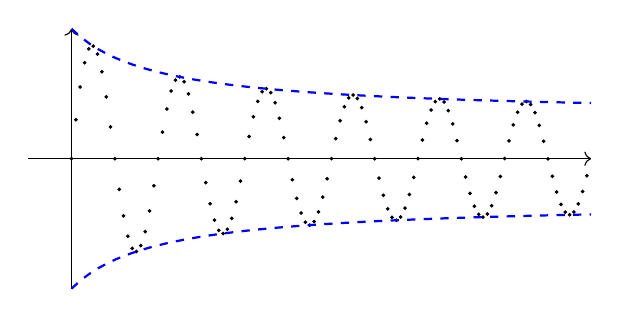
\begin{tikzpicture}[scale=1.1]
          \draw[->] (-0.5,0) -- (6,0);
          \draw[->] (0,-1.5) -- (0,1.5);
          
          % Draw the sine wave with smaller dots through exactly 5 periods
          \foreach \x in {0, 0.05, 0.1, ..., 6}
            \filldraw[black] (\x, {((1/(\x+1))+0.5)*sin(2*pi*\x r)}) circle (0.4pt); 

          \draw[blue, dashed, thick] plot[domain=0:6, samples=60] (\x, {1/(\x+1)+0.5});
          \draw[blue, dashed, thick] plot[domain=0:6, samples=60] (\x, {-1/(\x+1)-0.5});
        \end{tikzpicture}
        \caption{In order to find the limsup, we first look the whole sequence in $\mathbb{N}$ and find the supremum. We now "decrease" our domain from $\mathbb{N}$ to $\{2, \ldots\}$, then $\{3, \ldots\}$, then $\{4, \ldots\}$ and so on, continuing to label the supremum of the sequence. The limit of this sequence of supremums is the limsup.}
        \label{fig:limsupinf1}
      \end{subfigure}
      \hfill 
      \begin{subfigure}[b]{0.48\textwidth}
        \centering
        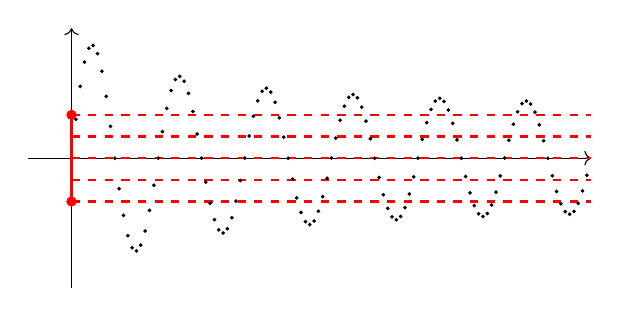
\begin{tikzpicture}[scale=1.1]
          \draw[->] (-0.5,0) -- (6,0);
          \draw[->] (0,-1.5) -- (0,1.5);
          \draw[-, red, dashed, thick] (0,0.5) -- (6,0.5);
          \draw[-, red, dashed, thick] (0,0.25) -- (6,0.25);
          \draw[-, red, dashed, thick] (0,0) -- (6,0);
          \draw[-, red, dashed, thick] (0,-0.25) -- (6,-0.25);
          \draw[-, red, dashed, thick] (0,-0.5) -- (6,-0.5);
          
          % Draw the sine wave with smaller dots through exactly 5 periods
          \foreach \x in {0, 0.05, 0.1, ..., 6}
            \filldraw[black] (\x, {((1/(\x+1))+0.5)*sin(2*pi*\x r)}) circle (0.4pt); 

          \draw[red, very thick] (0,-0.5) -- (0,0.5);
          \filldraw[red] (0,-0.5) circle (1.5pt);
          \filldraw[red] (0,0.5) circle (1.5pt);
        \end{tikzpicture}
        \caption{The 5 red lines marked in the middle (along with infinitely many others) are viable partial limits because one can choose a subsequence such that all of its points after a certain $n$ lie in some $\epsilon$-neighborhood of the limit. Therefore, we claim that the limsup/inf is the supremum of this set $E$.}
        \label{fig:limsupinf2}
      \end{subfigure}
      \caption{Two ways to visualize the superior and inferior limits of the divergent sequence $x_n = \big(\frac{1}{x+1} + 0.5\big) \sin(2\pi x)$. The left is the limit of the supremum, and the right is the supremum of the closed set of subsequential limits.} 
      \label{fig:limsupinf}
    \end{figure}
  \end{definition}

  \begin{example}[Computing Limsup and Liminf]
    We give some basic examples. 
    \begin{enumerate}
      \item Let $x_n = (-1)^n$. Then $E = \{-1, +1\}$ and 
      \begin{equation}
        \limsup_{n \rightarrow \infty} x_n = 1, \qquad \liminf_{n \rightarrow \infty} x_n = -1 
      \end{equation}

      \item Let $x_n = (-1)^n / [1 + (1/n)]$. Then 
      \begin{equation}
        \limsup_{n \rightarrow \infty} x_n = 1, \qquad \liminf_{n \rightarrow \infty} x_n = -1
      \end{equation}
    \end{enumerate}
  \end{example}

  Let's give two warnings. First, limsup and liminfs do \textit{not} behave like limits under addition and multiplication. That is, 
  \begin{equation}
    \limsup x_n + \limsup y_n \neq \limsup x_n + y_n 
  \end{equation}

  \begin{example}[Counterexamples of Arithmetic Consistency of Limit superior]
    Consider $(x_n) = (-1)^n$ and $y_n = (-1)^{n+1}$. Then 
    \begin{equation}
      \limsup x_n = \limsup y_n = 1, \qquad \liminf x_n = \liminf y_n = -1
    \end{equation}
    But $(x_n + y_n) = 0$, so 
    \begin{equation}
      \limsup x_n + y_n = \liminf x_n + y_n = 0 
    \end{equation}
  \end{example}

  Second, note that even though we are talking about subsequential limits, the limsup and liminf are \textit{not} subsequential limits! It is the supremum of subsequential limits $E$, which may or may not be in $E$. 

  \begin{example}[Limsup that is not attained by any subsequential limit]
    This should be a sequence not in $\mathbb{R}$. 
  \end{example}

  However, in $\mathbb{R}$, it turns out that the limsup and liminf are both contained in $E$, so we are fine. 

  \begin{lemma} 
    If $(x_n)$ is a sequence in $\mathbb{R}$, then 
    \begin{enumerate}
      \item the limsup is indeed a subsequential limit, i.e. $\limsup x_n \in E$. 
      \item If $x > \limsup x_n$, then $\exists N \in \mathbb{N}$ s.t. $n \geq N \implies x_n < x$. 
    \end{enumerate}
  \end{lemma}
  \begin{proof}
    For the first claim, there are two cases to consider. If $(x_n)$ is unbounded from above, then $\exists (x_{n_k})$ such that $x_{n_k} \rightarrow +\infty \implies \infty = \limsup x_n \in E$. If $(x_n)$ is bounded from above, then the subsequential limits of $(x_n)$ are either in $(x_n)$ or they are limit points of $x_n$. This implies that the set $E$ consists of points either in $\{x_n\}$ or are limit points of the set $\{x_n\} \implies \sup{E}$ is in $E$ since it's a limit point. 

    For the second claim, if there are infinitely many terms of the sequence larger than $x$, then we could find a subsequence $(x_{n_k})$ with $x_{n_k} > x$ for all $k$. Therefore $(x_n)$ has a subsequential limit which must be $\geq x$. Every subsequential limit of $(x_{n_k})$ is also a subsequential limit of $(x_n)$. This contradicts $\limsup x_n = \sup E$. 
  \end{proof}

  \begin{theorem}[Requirements of Partial Limits for Limit to Exist]
    Here are two results in which we can use partial limits to determine if a sequence has a limit or not. 
    \begin{enumerate}
      \item A sequence has a limit or tends to $\pm \infty$ if and only if its inferior and superior limits are the same. 
      \begin{equation}
        \limsup x_n = \liminf x_n = x \implies \lim_{n \rightarrow +\infty} x_n = x
      \end{equation}
      \item A sequence converges if and only if every subsequence of it converges. 
    \end{enumerate}
  \end{theorem}
  \begin{proof}
    For (1), we pick $x + \epsilon > x$. Then every term past some $N_1$ must be less than $x + \epsilon$. By the same logic, we have $N_2$ for $x - \epsilon < x$. So take $N = \max\{N_1, N_2\}$, which is contained in the $\epsilon$-ball around $x$. 
  \end{proof}

  \begin{theorem}[Ordering on Subsequential Limits]
    If $s_n \leq t_n$ for $n \geq N$, where $N$ is fixed, then 
    \begin{align*}
      \liminf_{n \rightarrow \infty} s_n & \leq \liminf_{n \rightarrow \infty} t_n \\
      \limsup_{n \rightarrow \infty} s_n & \leq \liminf_{n \rightarrow \infty} t_n 
    \end{align*}
  \end{theorem} 

  \begin{example}
    We claim 
    \begin{equation}
      \lim_{n \rightarrow \infty} n^{1/n} = 1 
    \end{equation}
    We can consider $x_n = n^{1/n} - 1$ and want to show that $x_n \rightarrow 0$. We have $x_n \geq 0$. If $n > 1$, then $n = (x_n + 1)^n \geq x_n^2 \cdot \frac{n(n - 1)}{2}$ from the binomial theorem. This means that 
    \begin{equation}
      x_n^2 \leq \frac{2}{n-1} \implies 0 \leq x_n \leq \sqrt{\frac{2}{n-1}} \rightarrow 0
    \end{equation}
    And so by the squeeze theorem, $x_n \rightarrow 0$. 
  \end{example}

  \begin{example}
    If $x > 1, \alpha \in \mathbb{R}$, then 
    \begin{equation}
      \lim_{n \rightarrow +\infty} \frac{n^\alpha}{x^n} = 0
    \end{equation} 
  \end{example}
 
\subsection{Convergence Tests for Real Series}

  \begin{definition}[Series over $\mathbb{R}$]
    Given a sequence of real numbers $(x_n)$, the \textbf{series (of partial sums)} is the sequence 
    \begin{equation}
      (s_n) = \sum_{k=1}^n x_k
    \end{equation}
    The \textbf{sum of the series} is the limit of $(s_n)$. Usually we define $(s_n)$ implicitly and use the summation notation. 
    \begin{equation}
      \sum_{n=1}^\infty x_n \coloneqq \lim_{n \rightarrow \infty} s_n
    \end{equation}
    \begin{enumerate}
      \item If the sequence $(s_n)$ converges to $s$, the series is \textbf{convergent}, written 
      \begin{equation}
        \sum x_n < +\infty
      \end{equation}
      \item If the sequence does not converge, it is \textbf{divergent}. 
      \item If the series of partial sums of $(|x_n|)$ converges, then it is said to be \textbf{absolutely convergent}.\footnote{Clearly, every absolutely convergent series because $\big|\sum_{n=1}^\infty a_n \big| \leq \sum_{n=1}^\infty |a_n|$. }
      \begin{equation}
        \sum_{n=1}^\infty |x_n|
      \end{equation}
    \end{enumerate}
  \end{definition}

  We must reiterate a few warnings here. Note that the series $\sum x_n$ is simply notation and should \textit{not} be treated as an ``infinite sum.'' Such a thing does not exist for algebraic structures which have finary operations. More specifically, given a series, we cannot in general split nor combine series, and we cannot reindex nor rearrange (an infinite number of) terms. However, we can manipulate each term for a fixed index. 

  \begin{example}[Disasters of Reindexing and Rearranging]
    Let us take the series $\sum 0$. We clearly know that the corresponding sequence of partial sums $0, 0, \ldots$ is convergent to $0$. But if we do this series of steps. 
    \begin{align}
      \sum_{n=1}^\infty 0 & = \sum_{n=1}^\infty n - n && \tag{Can manipulate terms} \\
                          & = \sum_{n=1}^\infty n - \sum_{n=1}^\infty n && \tag{Cannot split series} \\ 
                          & = 1 + \sum_{n=2}^\infty n - \sum_{n=1}^\infty n && \tag{Can take 1st term out} \\ 
                          & = 1 + \sum_{n=1}^\infty (n+1) - \sum_{n=1}^\infty n && \tag{Cannot reindexing} \\
                          & = 1 + \sum_{n=1}^\infty (n+1) - n  && \tag{Cannot combine series} \\
                          & = 1 + \sum_{n=1}^\infty 1 && \tag{Can manipulate terms} \\
                          & = 1 + \infty = +\infty
    \end{align}
    The wrong steps show that the series is divergent. 
  \end{example} 

  We have seen the consequences of these mistakes that beginners make and are often on popular media. However, note that we can always do splitting, combining, reindexing, and rearranging for \textit{finite sums}, which are algebraically defined. Later on, we will show that some of these operations are allows for series that we know are convergent.  

  Since the convergence of a series is equivalent to convergence of its sequence of partial sums, applying the Cauchy convergence criterion to the sequence $\{s_n\}$ leads to the following theorem. 

  \begin{theorem}[Cauchy Convergence Criterion for Series]
    The series $a_1 + \ldots + a_n + \ldots$ converges if and only if for every $\epsilon > 0$ there exists $N \in \mathbb{N}$ such that for all $m \geq n > N$, 
    \begin{equation}
      |a_n + \ldots + a_m| < \epsilon
    \end{equation}
  \end{theorem}

  \begin{corollary}[nth Term Test]
    A necessary (but not sufficient) condition for convergence of the series $a_1 + \ldots a_n + \ldots$ is that the terms tend to $0$ as $n \rightarrow \infty$. That is, it is necessary that
    \begin{equation}
      \lim_{n\rightarrow \infty} a_n = 0
    \end{equation}
  \end{corollary}
  \begin{proof}
    It suffices to set $m = n$ in the Cauchy convergence criterion. This would mean that for every $\epsilon > 0$ there exists a $N \in \mathbb{N}$ such that 
    \begin{equation}
      |a_n| = |a_n - 0| < \epsilon \text{ for all } n > N
    \end{equation}
    which, by definition, means that $\{a_n\}$ converges to $0$. 
  \end{proof} 

  Nothing so far is really suprising here. The Cauchy convergence criterion really just follows from the definition of Cauchy completeness, and the $n$th term test is pretty trivial. The way that we will build up convergence tests is by proving some special cases of convergence and then using the direct comparison test to then classify further series.     

  \begin{example}[Telescoping Series]
    A \textbf{telescoping series} is a series in which the partial sums can cancel out. An example is the series of partial sums of the sequence $(x_n) = \frac{1}{n (n+1)}$. In here, the series term is
    \begin{align}
      s_n & = \sum_{k=1}^n \frac{1}{k(k+1)} \\ 
          & = \sum_{k=1}^n \frac{1}{k} - \frac{1}{k+1} \\
          & = \sum_{k=1}^n \frac{1}{k} - \sum_{k=1}^n \frac{1}{k+1} \\
          & = \sum_{k=1}^n \frac{1}{k} - \sum_{k=2}^{n+1} \frac{1}{k} \\
          & = \frac{1}{1} + \bigg( \sum_{k=2}^n \frac{1}{k} \bigg) - \bigg( \sum_{k=2}^n \frac{1}{k} \bigg) - \frac{1}{n+1} \\
          & = 1 + \bigg( \sum_{k=2}^n \frac{1}{k} - \frac{1}{k} \bigg) - \frac{1}{n+1} \\
          & = 1 - \bigg( \sum_{k=2}^n 0 \bigg) - \frac{1}{n+1} \\
          & = 1 - \frac{1}{n+1} 
    \end{align} 
    Note that all of the examples that we have done here are for finite sums, so they are all legal. 
  \end{example}

  \begin{example}[Geometric Series]
    The series $\sum_{n=0}^\infty q^n$ is called a \textbf{geometric series}. 
    \begin{equation}
      1 + q + q^2 + \ldots + q^n + \ldots
    \end{equation}
    is called the \textbf{geometric series}. We can see that 
    \begin{enumerate}
      \item $|q| \geq 1 \iff \sum q^n$ is divergent. $|q| \geq 1 \implies |q|^n \geq 1$, and so the terms $q^n$ does not converge to $0$, and the $n$th term test is not met. 
      \item $|q| < 1 \iff \sum q^n$ is convergent. We can use the identity 
      \begin{equation}
        s_n = 1 + q + \ldots + q^{n-1} = \frac{1 - q^n}{1-q} \implies \lim_{n \rightarrow \infty} \frac{1 - q^n}{1 - q} = \frac{1}{1 - q}
      \end{equation} 
      since $\lim_{n\rightarrow \infty} q^n = 0$ if $|q|<1$. 
    \end{enumerate}
  \end{example}

  The Cauchy convergence criterion can be used to prove the direct comparison test. 

  \begin{theorem}[Direct Comparison Test] 
    For some fixed $N$, if 
    \begin{enumerate}
      \item If $|x_n| \leq y_n$ for all $n \geq N$ and $\sum y_n$ converges, then $\sum x_n$ converges. 
      \item If $x_n \geq y_n \geq 0$ for all $n \geq N$  and $\sum y_n$ diverges, then $\sum x_n$ diverges. 
    \end{enumerate}
  \end{theorem} 

  \begin{example}[Comparison with Telescoping Series]
    We can prove the special case a geometric series with the direct comparison test. We claim that $\sum_{n=1}^\infty \frac{1}{n^2}$ is finite. We can see that 
    \begin{equation}
      \frac{1}{n^2} \leq \frac{2}{n (n+1)} 
    \end{equation}
    where the series of the terms in the RHS is telescoping and therefore converges. So by the direct comparison test, $\sum \frac{1}{n^2}$ converges. 
  \end{example}

  Now we prove another corollary of the Cauchy convergence criterion.   

  \begin{theorem}[Cauchy Condensation Test]
    If $a_1 \geq a_2 \geq \ldots \geq 0$, the series $\sum_{n=1}^\infty a_n$ converges if and only if the series 
    \begin{equation}
      \sum_{k=0}^\infty 2^k a_{2^k} = a_1 + 2 a_2 + 4a_4 + 8a_8 + \ldots 
    \end{equation}
    converges. 
  \end{theorem}
  \begin{proof}
    Letting $A_k = a_1 + a_2 + \ldots + a_k$ and $S_n = a_1 + 2a_2 + \ldots + 2^n a_{2^n}$, it is clear that by adding up the inequalities
    \begin{align*}
      & a_2 \leq a_2 \leq a_1 \\
      & 2a_4 \leq a_3 + a_4 \leq 2a_2 \\
      & 4a_8 \leq a_5 + a_6 + a_7 + a_8 \leq 4a_4 \\
      & \ldots \\
      & 2^n a_{2^{n+1}} \leq a_{2^n + 1} + \ldots + a_{2^{n+1}} \leq 2^n a_{2^n}, 
    \end{align*}
    we get
    \begin{equation}
      \frac{1}{2}(S_{n+1} - a_1) \leq A_{2^{n+1}} - a_1 \leq S_n
    \end{equation}
    Since the sequences $\{A_k\}$ and $\{S_k\}$ are nondecreasing, and hence from the inequalities we can conclude that they are either both bounded above (which means that they are both convergent since it is a bounded, nondecreasing series) or both unbounded above (which means that they are both divergent since they are nondecreasing and unbounded). 
  \end{proof}

  \begin{corollary}[p-series Test]
    The series 
    \begin{equation}
      \sum_{n=1}^\infty \frac{1}{n^p}
    \end{equation}
    converges for $p>1$ and diverges for $p \leq 1$.\footnote{This sort of reminds you of $u$-substitution. For example, look at $\int_1^\infty f(t) \,dt = \int_0^\infty e^u f(e^u)\,du$, where the convergence of LHS $\iff$ convergence of RHS.}
  \end{corollary}
  \begin{proof}
    Suppose $p\geq 0$. By the previous theorem, the series converges or diverges simultaneously with the series 
    \begin{equation}
      \sum_{k=0}^\infty 2^k \frac{1}{(2^k)^p} = \sum_{k=0}^\infty (2^{1-p})^k
    \end{equation}
    which is really just a geometric series. A necessary and sufficient condition for the convergence of this series is that $2^{1-p} < 1$, that is, $p>1$. 

    Now suppose $p \leq 0$. The series is then clearly divergent since all of the terms are larger than $1$. 
  \end{proof}

  \begin{example}[Harmonic Series]
    The \textbf{harmonic series} 
    \begin{equation}
      1 + \frac{1}{2} + \frac{1}{3} + \ldots + \frac{1}{n} + \ldots
    \end{equation}
    seems at first glance to be converging since the terms converge to $0$. However, it does not pass the Cauchy condensation test since 
    \begin{equation}
      \sum_{n=1}^\infty 2^n x_n = \sum_{n=1}^\infty 2^n \frac{1}{2^n} = \sum_{n=1}^\infty 1 = +\infty
    \end{equation}
    As you can see, this increases logarithmically, so in early calculators it was hard to numerically detect divergence (you would have to double the number of series terms to get a linear increase). 
  \end{example} 

\subsection{Ratio and Root Tests} 

  Now we introduce the root and ratio tests, which are derived by the comparison test with a geometric series. The ratio test is used more day-to-day, but not as decisive as the root test. Both tests have a similar flavor. 

  \begin{theorem}[Ratio Test]
    Suppose the limit $\lim_{n\rightarrow \infty} \big| \frac{a_{n+1}}{a_n} \big| = \alpha$ exists for the series $\sum_{n=1}^\infty a_n$. Then, 
    \begin{enumerate}
      \item $\alpha < 1 \implies \sum a_n$ converges absolutely. 
      \item $\alpha > 1 \implies \sum a_n$ diverges.
      \item $\alpha = 1 \implies \sum a_n$ is inconclusive. 
    \end{enumerate}
    Alternatively, if 
    \begin{enumerate}
      \item $\limsup |a_{n+1}/a_n| = \alpha < 1$, then $\sum a_n$ converges 
      \item If $\exists N$ s.t. $|a_{n+1}/a_n| \geq 1$ for all $n \geq N$, then $\sum a_n$ diverges. 
    \end{enumerate}
  \end{theorem}
  \begin{proof}
    Since $\limsup \big| \frac{a_{n+1}}{a_n} \big| = \alpha < 1$, fix any $\alpha < \beta < 1$. Then $\exists N$ s.t. if $n > N$, $|a_{n+1}/a_n| < \beta$. So $|a_{N+1}| < \beta |a_N| \implies |a_{N+2}| < \beta^2 |a_N|$. So letting $C = |a_N|$, for all $m \geq N$, 
    \begin{equation}
      |a_m| \leq \frac{C}{\beta^N} \beta^m \implies |a_m| \leq \Tilde{C} \beta^m \text{ for all } m \geq N
    \end{equation}
    So $\sum a_n$ converges by comparison test since $\sum \beta^m < \infty$ when $\beta < 1$. 
  \end{proof}

  \begin{theorem}[Root Test]
    Let $\sum_{n=1}^\infty a_n$ be a given series and 
    \begin{equation}
      \alpha = \limsup_{n\rightarrow \infty} \sqrt[n]{|a_n|}
    \end{equation}
    Then, 
    \begin{enumerate}
      \item $\alpha < 1 \implies \sum a_n$ converges. 
      \item $\alpha > 1 \implies \sum a_n$ diverges. 
      \item $\alpha = 1 \implies \sum a_n$ is inconclusive. 
    \end{enumerate}
  \end{theorem} 
  \begin{proof}
    Listed. 
    \begin{enumerate}
      \item If $\limsup \sqrt[n]{|a_n|} = \alpha < 1$, take any $\alpha < \beta < 1$. Then $\exists N \in \mathbb{N}$ s.t. if $n \geq N$, then $|a_n|^{1/n} < \beta \iff |a_n| < \beta^n$. Since $\beta < 1$, $\sum \beta^n < \infty$, and by comparison test, $\sum a_n$ converges. 

      \item Suppose $\alpha > 1$. Then $\limsup |a_n|^{1/n} = \alpha > 1$. So there exists a subsequence $(a_{n_k})$ s.t. $(|a_{n_k}|^{1/n_k}) \rightarrow \alpha > 1$. This means $\exists N$ s.t. for $n \geq N$, $|a_{n_k}|^{1/{n_k}} > 1 \implies |a_{n_k}| > 1$. But this fails the $n$th term test. 

      \item We do not claim anything and so there's nothing to prove. 
    \end{enumerate}
  \end{proof}

  \begin{example}[Root Test Inconclusive Results]
    Consider $\sum \frac{1}{n} = +\infty$, but from the root test 
    \begin{equation}
      \sqrt[n]{\frac{1}{n}} \rightarrow 1, \text{ so } \alpha = 1
    \end{equation}
    Consider $\sum \frac{1}{n^2} < +\infty$, but from from the root test 
    \begin{equation}
      \sqrt[n]{\frac{1}{n^2}} = \bigg( \frac{1}{n^{1/n}} \bigg)^2 \rightarrow 1, \text{ so } \alpha = 1
    \end{equation}
  \end{example}

  \begin{example}
    The sequence $\sum \frac{c^n}{n!}$ always converges for $c \in \mathbb{R}$. 
  \end{example}

  \begin{theorem}[Weierstrass M-test for Absolute Convergence]
    Let $\sum_{n=1}^\infty a_n$ and $\sum_{n=1}^\infty b_n$ be series. Suppose there exists an index $N \in \mathbb{N}$ such that $|a_n| \leq b_n$ for all $n>N$. Then, 
    \begin{equation}
      \sum_{n=1}^\infty b_n \text{ converges } \implies \sum_{n=1}^\infty a_n \text{ converges absolutely}
    \end{equation}
  \end{theorem}

  We finally conclude by giving a theorem about the convergence of some special sequences. 

  \begin{theorem}[Special Sequences]
    Some special sequences: 
    \begin{enumerate}
      \item If $p > 0$, then $\lim_{n \rightarrow \infty} \frac{1}{n^p} = 0$. 
      
      \item If $p > 0$, then $\lim_{n \rightarrow \infty} \sqrt[n]{p} = 1$. 

      \item $\lim_{n \rightarrow \infty} \sqrt[n]{n} = 1$. 

      \item If $p > 0$ and $\alpha$ is real, then $\lim_{n \rightarrow \infty} \frac{n^\alpha}{(1 + p)^n} = 0$. 
      
      \item If $|x| < 1$, then $\lim_{n \rightarrow \infty} x^n = 0$. 
    \end{enumerate}
  \end{theorem}

\subsection{Euler's Number and Trigonometric Functions} 

  \begin{definition}[Euler's Number]
    We define \textbf{Euler's number} as 
    \begin{equation}
      e \coloneqq \sum_{n=0}^\infty \frac{1}{n!}
    \end{equation}
  \end{definition}
  
  The first thing we should do is show that it converges, this is a one-liner. 
  \begin{equation}
    \sum_{n=0}^\infty \frac{1}{n!} = 1 + 1 + \sum_{n=2}^\infty \frac{1}{n!} \leq 2 + \sum_{n=2}^\infty \frac{1}{n(n-1)} 
  \end{equation}

  \begin{theorem}[Euler's Number as a Limit]
    We have 
    \begin{equation}
      \lim_{n \rightarrow +\infty} \bigg( 1 + \frac{1}{n} \bigg)^n = e 
    \end{equation}
  \end{theorem}
  \begin{proof}
    Let us define the sequence 
    \begin{equation}
      t_n = \sum_{k=0}^n \frac{1}{k!}, \qquad s_n = \bigg( 1 + \frac{1}{n} \bigg)^n
    \end{equation}
    We know that $t_n \rightarrow e$, and we want to show that $s_n \rightarrow e$. We do this with the squeeze theorem. 
    \begin{enumerate}
      \item We can see that 
      \begin{align}
        s_n & = \bigg( 1 + \frac{1}{n} \bigg)^n \\ 
            & = \sum_{k=0}^n \binom{n}{k} 1^{n-k} \bigg( \frac{1}{n} \bigg)^k \\
            & = 1 + 1 + \frac{n(n-1)}{2!} \frac{1}{n^2} + \frac{n(n-1)(n-2)}{3!} \frac{1}{n^3} + \ldots \\ 
            & = 1 + 1 + \frac{1}{2!} (1) \bigg( 1 - \frac{1}{n} \bigg) + \frac{1}{3!} (1) \bigg(1 - \frac{1}{n} \bigg) \bigg(1 - \frac{2}{n} \bigg) + \ldots + \frac{1}{n!} (1) \prod_{k=1}^{n-1} \bigg(1 - \frac{k}{n} \bigg) \\
            & \leq \frac{1}{0!} + \frac{1}{1!} + \frac{1}{2!} + \frac{1}{3!} + \ldots + \frac{1}{n!} = t_n 
      \end{align}
      and so $s_n < t_n \implies \limsup s_n \leq \limsup t_n = e$. 

      \item Let $m \leq n$ be fixed. Then, 
      \begin{equation}
        s_n \geq 1 + 1 + \frac{1}{2!} \bigg( 1 - \frac{1}{n} \bigg) + \ldots + \frac{1}{m!} \bigg(1 - \frac{1}{n} \bigg) \bigg(1 - \frac{2}{n} \bigg) \ldots \bigg(1 - \frac{m-1}{n} \bigg) 
      \end{equation}
      since we are just taking the first $m$ positive terms of the element. Therefore, letting $n \rightarrow +\infty$ and keeping $m$ fixed, we get 
      \begin{equation}
        \liminf_{n \rightarrow +\infty} s_n \geq 1 + 1 + \frac{1}{2!} + \ldots + \frac{1}{n!} \text{ for all } m \in \mathbb{N}
      \end{equation}
      which implies $\liminf s_n \geq t_m$ for all $m \in \mathbb{N}$, and now letting $m \rightarrow +\infty$, we have $\liminf s_n \geq \liminf t_m = e$. 
    \end{enumerate}
  \end{proof}

  Now we prove the irrationality of $e$. It is usually extremely difficult to prove that an arbitrary number is irrational, e.g. $\pi^e$ or $\pi^{e^e}$. 

  \begin{theorem}[$e$ is Irrational]
    $e$ is irrational. 
  \end{theorem}
  \begin{proof} 
    Letting $t_n = \sum_{k=0}^n \frac{1}{k!}$, we have 
    \begin{align}
      e - t_n & = \sum_{k=n+1}^\infty \frac{1}{k!} \\
              & = \frac{1}{(n+1)!} \bigg( 1 + \frac{1}{n+2} + \frac{1}{(n+3)(n+2)} + \ldots \bigg) \\
              & < \frac{1}{(n+1)!} \underbrace{\bigg( 1 + \frac{1}{n+2} + \frac{1}{(n+2)^2} + \ldots \bigg)}_{\text{geometric}} \\
              & = \frac{1}{(n+1)!} \bigg( \frac{1}{1 - (1/(n+2)!)}\bigg) \\
              & = \frac{1}{n! n} \cdot \underbrace{\frac{(n+2) n}{(n+1)^2}}_{< 1} \\
              & = \frac{1}{n! n}
    \end{align}
    Note that we can combine and split sums since we know that $e$ is convergent. Now suppose that $e = p/q$. Then, 
    \begin{equation}
      0 < q! (e - t_q) < \frac{1}{q}
    \end{equation}
    But $q! e$ is an integer and $q! t_q$ is also an integer. So we have $q! \cdot \frac{p}{q}$, an integer, between $0$ and $1$, which is a contradiction. 
  \end{proof}

  Since we have defined some number $e \in \mathbb{R}$, we know that exponential exist, and therefore we the function $x \mapsto e^x$ is well-defined. In fact, it is so important that we have a separate name for it. 

  \begin{definition}[Exponential Function]
    The \textbf{exponential function} is generally referred to as the function $x \mapsto e^x$. 
  \end{definition}

  There is a nice series representation. 

  \begin{theorem}[Exponential Function as a Series]
    We have 
    \begin{equation}
      e^x = \sum_{n=0}^\infty \frac{x^n}{n!}
    \end{equation}
  \end{theorem}
  \begin{proof}
    
  \end{proof}

  Now that this is done, we can define the trigonometric functions formally as such. 

  \begin{definition}[Trigonometric Functions]
    We have 
    \begin{align}
      \sin x&=\sum_{n=0}^{\infty}\frac{(-1)^n}{(2n+1)!}x^{2n+1}=x-\frac{x^3}{3!}+\frac{x^5}{5!}-\cdots
      \\\\
      \cos x&=\sum_{n=0}^{\infty}\frac{(-1)^n}{(2n)!}x^{2n}=1-\frac{x^2}{2!}+\frac{x^4}{4!}-\cdots
    \end{align}
  \end{definition}


 
\section{Limits and Continuity of Functions} 

  We now extend our analysis to real-valued functions over a metric space. The ones that we will be particularly interested in are \textit{continuous functions}. But before this, let's introduce a new notation. Given a metric space $X$, we will talk about a variable $x$ approaching a particular value $a \in X$, denoted $x \rightarrow a$. But this isn't clear. When we talk about the concept of something approaching another thing, we have two definitions. 
  \begin{enumerate}
    \item A \textit{sequence} can approach to its limit, which is a \textit{point}. 
    \item A \textit{point} can be a limit point of a \textit{set}. 
  \end{enumerate} 
  When we write $x \rightarrow a$, we are talking about some indeterminate variable $x$ and a point $a$, it isn't immediately clear what this means. As we will soon define, this will refer to a neighborhood of $a$ or equivalently to \textit{all} sequences converging to $a$. So we can think of $x \rightarrow a$ as notation for all sequences $(x_n) \rightarrow a$.   

  \begin{definition}[Constant and Ultimately Constant Functions]
    Given a real-valued function $f: E \longrightarrow \mathbb{R}$ defined on domain $E \subset \mathbb{R}$,
    \begin{enumerate}
      \item $f$ is a \textbf{constant function} if $f(x) = A$ for all $x \in E$
      \item $f$ is called \textbf{ultimately constant} as $x \rightarrow a$ if it is constant in some deleted neighborhood $\mathring{U} (a)$, where $a$ is a limit point of $E$.
    \end{enumerate}
  \end{definition} 

  \begin{definition}[Bounded and Ultimately Bounded Functions]
    Given a real-valued function $f: E \longrightarrow \mathbb{R}$ defined on domain $E \subset \mathbb{R}$,
    \begin{enumerate}
      \item $f$ is \textbf{bounded}, \textbf{bounded above}, or \textbf{bounded below} respectively if there is a number $C \in \mathbb{R}$ such that $|f(x)|<C$, $f(x)<C$, or $C<f(x)$ for all $x \in E$.

      \item $f$ is \textbf{ultimately bounded}, \textbf{ultimately bounded above}, or \textbf{ultimately bounded below} as $x \rightarrow a$ if it is bounded, bounded above, or bounded below in some deleted neighborhood $\mathring{U}_E (a)$. 
    \end{enumerate}
  \end{definition}

  \begin{example}[Unbounded but Ultimately Bounded]
    The function 
    \begin{equation}
      f(x) = \sin{\frac{1}{x}} + x \cos{\frac{1}{x}}
    \end{equation}
    for $x \neq 0$ is not bounded on the domain of definition, but it is ultimately bounded as $x \rightarrow 0$. 
  \end{example}

\subsection{Limits of Functions}

  \begin{definition}[Limit of a Function]
    Let $f: X \rightarrow Y$ be a map between metric spaces, with $E \subset X$ and  $p \in E^\prime$ (note the limit point!). We say $f(x) \rightarrow q$ as $x \rightarrow p$, i.e. 
    \begin{equation}
      \lim_{x \rightarrow p} f(x) = q
    \end{equation} 
    if it meets the following equivalent conditions. 
    \begin{enumerate}
      \item \textit{$\epsilon$-$\delta$ Definition}. If $\forall \epsilon > 0$, $\exists \delta > 0$ s.t. $0 < d_X (x, p) < \delta \implies d_Y (f(x), q)) < \epsilon$.\footnote{Note that the strictly inequality $0 < d_X (x, p)$ is important to ensure that $x \neq p$, since functions can jump at $p$.} 

      \begin{figure}[H]
        \centering 
        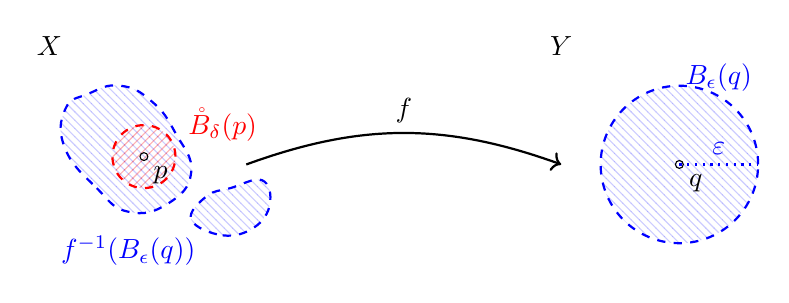
\begin{tikzpicture}
          \node at (0, 3) {$X$};
          \node at (6.5, 3) {$Y$};
          
          % Function arrow
          \draw[->, thick, bend left=20] (2.5,1.5) to node[above] {$f$} (6.5,1.5);
          
          % Blue blob 1 - made bigger but still in top left
          \draw[blue, thick, dashed] plot [smooth cycle, tension=0.8] coordinates {(0.2,1.7) (0.6,1.2) (1.0,0.9) (1.5,1.0) (1.8,1.4) (1.6,1.9) (1.3,2.3) (0.9,2.5) (0.5,2.4) (0.2,2.2)};
          \fill[blue, pattern=north west lines, pattern color=blue, opacity=0.2] plot [smooth cycle, tension=0.8] coordinates {(0.2,1.7) (0.6,1.2) (1.0,0.9) (1.5,1.0) (1.8,1.4) (1.6,1.9) (1.3,2.3) (0.9,2.5) (0.5,2.4) (0.2,2.2)};
          \node at (1.0,0.4) [blue] {$f^{-1}(B_\epsilon(q))$};
          
          % Blue blob 2 - in bottom right
          \draw[blue, thick, dashed] plot [smooth cycle, tension=0.7] coordinates {(1.8,0.8) (2.2,0.6) (2.6,0.7) (2.8,1.0) (2.7,1.3) (2.3,1.2) (2.0,1.1)};
          \fill[blue, pattern=north west lines, pattern color=blue, opacity=0.2] plot [smooth cycle, tension=0.7] coordinates {(1.8,0.8) (2.2,0.6) (2.6,0.7) (2.8,1.0) (2.7,1.3) (2.3,1.2) (2.0,1.1)};
          
          % Left neighborhood (red, hatched circle) - moved inside V1
          \draw[red, thick, dashed] (1.2,1.6) circle (0.4);
          \fill[red, pattern=north east lines, pattern color=red, opacity=0.3] (1.2,1.6) circle (0.4);
          \node at (2.2,2) [red] {$\mathring{B}_\delta(p)$};
          
          % Point p - hollow and red - also moved
          \draw (1.2,1.6) circle (0.05);
          \node at (1.2,1.6) [below right] {$p$};
          
          % Right neighborhood (blue circle)
          \draw[blue, thick, dashed] (8,1.5) circle (1);
          \fill[blue, pattern=north west lines, pattern color=blue, opacity=0.2] (8,1.5) circle (1);
          \node at (8.5,2.6) [blue] {$B_\epsilon(q)$};
          
          % Point q - where f(p) would be, now just a point reference
          \draw (8,1.5) circle (0.05);
          \node at (8,1.5) [below right] {$q$};
          
          % Epsilon visualization - dotted line segment not touching the blue boundary
          \draw[blue, thick, dotted] (8,1.5) -- (9,1.5) node[midway, above] {$\varepsilon$};
        \end{tikzpicture}
        \caption{Said in one line, the preimage of any open ball around $y = f(x)$ must contain some open deleted open ball around $x$.} 
        \label{fig:limit_function}
      \end{figure}

      \item \textit{Sequential Definition}. If for all sequences $(x_n) \rightarrow p$, $f(x_n) \rightarrow q$.

      \begin{figure}[H]
        \centering 
        \begin{tikzpicture}[scale=1]
          % Space labels without axes
          \node at (1, 3) {$X$};
          \node at (7.5, 3) {$Y$};
          
          % Function arrow
          \draw[->, thick, bend left=20] (3.5,1.5) to node[above] {$f$} (7.5,1.5);
          
          % Point a in domain - shifted by 1
          \fill (2.5,1.5) circle (0.07);
          \node at (2.5,1.5) [above right] {$p$};
          
          % Blue sequence (x_n) in domain - curved path - shifted by 1
          \filldraw[blue] (1.3,0.6) circle (0.03);
          \filldraw[blue] (1.7,0.8) circle (0.03);
          \filldraw[blue] (1.9,1.0) circle (0.03);
          \filldraw[blue] (2.1,1.3) circle (0.03);
          \filldraw[blue] (2.3,1.4) circle (0.03);
          \node at (1.6,0.4) [blue] {$(x_n)$};
          
          % Red sequence (y_n) in domain - curved path - shifted by 1
          \filldraw[red] (2.7,1.6) circle (0.03);
          \filldraw[red] (2.9,1.7) circle (0.03);
          \filldraw[red] (3.0,1.8) circle (0.03);
          \filldraw[red] (3.2,1.85) circle (0.03);
          \filldraw[red] (3.5,1.9) circle (0.03);
          \node at (3.4,2.0) [red] {$(y_n)$};
          
          % Point A in codomain
          \fill (8,1.5) circle (0.07);
          \node at (8,1.5) [above right] {$q$};
          
          % Blue sequence (f(x_n)) in codomain - curved path
          \filldraw[blue] (7.1,0.7) circle (0.03);
          \filldraw[blue] (7.3,0.9) circle (0.03);
          \filldraw[blue] (7.5,1.1) circle (0.03);
          \filldraw[blue] (7.7,1.2) circle (0.03);
          \filldraw[blue] (7.8,1.4) circle (0.03);
          \node at (7.2,0.4) [blue] {$(f(x_n))$};
          
          % Red sequence (f(y_n)) in codomain - curved path
          \filldraw[red] (8.2,1.7) circle (0.03);
          \filldraw[red] (8.5,1.8) circle (0.03);
          \filldraw[red] (8.7,2.0) circle (0.03);
          \filldraw[red] (8.9,2.3) circle (0.03);
          \filldraw[red] (9.1,2.5) circle (0.03);
          \node at (9.2,1.9) [red] {$(f(y_n))$};
        \end{tikzpicture}
        \caption{For every sequence that converges to the left, the new sequence mapped through $f$ converges to $q$. Note that we choose the points $x_n$ to be in the "deleted" neighborhood $E\setminus a$ (neighborhood $E$ with point $a$ removed) to force us to choose a sequence that is not $a, a, \ldots$. That is, it forces us to choose different points for the sequence. } 
        \label{fig:sequential_limit_def}
      \end{figure}
    \end{enumerate}
  \end{definition}
  \begin{proof}
    We prove equivalence. 
    \begin{enumerate}
      \item $(\rightarrow)$. Assume $\lim_{x \rightarrow p} f(x) = q$. Let $(x_n) \in E$ s.t. $x_n \rightarrow p$ with $x_n \neq p$. We wish to show that $f(x_n) \rightarrow q$. Let $\epsilon > 0$. Then $\exists \delta > 0$ s.t. $0 < d_X (x, p) < \delta \implies d_Y (f(x), q) < \epsilon$. Since $\delta > 0$, by definition $\exists N \in \mathbb{N}$ s.t. if $n \geq N$, $d_X (x_n , p) < \delta \implies d_Y (f(x_n), q)$. 
    \end{enumerate}
  \end{proof}

  Sometimes, the $\epsilon$-$\delta$ definition is good, but a lot of the times the sequential definition is good enough and more insightful. 

  \begin{example}[Limit of the Signum Function]
    The function sgn$: \mathbb{R} \longrightarrow \mathbb{R}$ defined
    \begin{equation}
      \text{sgn}\,x = \begin{cases} 1, & x > 0 \\ 0, & x = 0 \\ -1, & x < 0 \end{cases}
    \end{equation}
    has no limit as $x \rightarrow 0$. 

    First, it is ludicrous that the limit would be any number that is not $\{-1, 0, 1\}$. If we assume that $A \not\in \{-1,0,1\}$, then we can choose any arbitrarily small $\epsilon$-neighborhood of $A$ that does not include the three numbers. Clearly, there doesn't exist any $\delta>0$ such that the deleted $\delta$-neighborhood of $0$ maps to a set completely contained in the $\epsilon$-neighborhood of $A$. That is,
    \begin{equation}
      \text{sgn}\big( \mathring{U}_\delta (0)\big) = \{-1,1\} \not\subset U_\epsilon (A)
    \end{equation}
    It doesn't even intersect the $\epsilon$-neighborhood at all. 
    \begin{enumerate}
      \item If $A = 1$, we can construct a $\epsilon$-neighborhood $V_A$ for $\epsilon = \frac{1}{2}$. Clearly, there exists no open neighborhood $U_0$ of $0$ that is entirely mapped to $V$, since $U_0$ contains both negative numbers and $0$ and hence must be mapped to $0, -1$. 
      \item Similarly, given the $(\epsilon=\frac{1}{2})$-neighborhood of $A = -1$, there exists no open neighborhood $U_0$ of $0$ that is entirely mapped to it, since $U_0$ contains both positive numbers and $0$ and hence must be mapped to $0, 1$. 
      \item Finally, given the $(\epsilon=\frac{1}{2})$-neighborhood of $A = 0$, there exists no open neighborhood $U_0$ of $0$ that is entirely mapped to it, since $U_0$ contains both positive and negative numbers and hence must be mapped to $\pm1$. 
    \end{enumerate}
    Therefore, the limit does not exist. 
  \end{example}

  \begin{example}[Limit of Absolute Value of Signum Function]
    We will show that 
    \begin{equation}
      \lim_{x \rightarrow 0} |\text{sgn}\,x| = 1
    \end{equation}
    We construct a $\epsilon$-neighborhood $U_\epsilon (1)$ around $1$. Given this neighborhood, we can imagine choosing the deleted $\delta$-neighborhood $\mathring{U}_\delta (0)$ around $0$. Since every element in $\mathring{U}_\delta (0)$ maps to $1$, it is clearly in $U_\epsilon$. In fact, for arbitrarily small $\epsilon > 0$, we can choose \textbf{any} $\delta>0$ since everything in $\mathbb{R} \setminus 0$ maps to $1$. We can visualize this in $\mathbb{R}^2$ as
  \end{example}

  \begin{theorem}[Arithmetic on Limits of Functions]
    Given two numerical valued functions $f, g: E \subset \mathbb{R} \longrightarrow \mathbb{R}$ with a common domain where $g(x) \neq 0$ for all $x \in E$, let 
    \begin{equation}
      \lim_{x \rightarrow a} f(x) = A, \;\;\;\;\; \lim_{x \rightarrow a} g(x) = B
    \end{equation}
    then, 
    \begin{align*}
      & \lim_{x \rightarrow a} (f+g)(x) = A + B \\
      & \lim_{x \rightarrow a} (cf)(x) = cA \\
      & \lim_{x \rightarrow a} (f \cdot g)(x) = A \cdot B \\
      & \lim_{x \rightarrow a} \bigg(\frac{f}{g}\bigg) (x) = \frac{A}{B}
    \end{align*}
  \end{theorem}
  \begin{proof}
    Cauchy sequence criterion for a limit immediately proves this. 
  \end{proof}

  We end this with a theorem connecting the relationship between a limit of a function as $x \rightarrow a$ and its ultimate behavior as $x \rightarrow a$. 

  \begin{theorem}
    Let $f: E \longrightarrow \mathbb{R}$ be a function. Then, 
    \begin{enumerate}
      \item $f$ is ultimately the constant $A$ as $x \rightarrow a$ implies that $\lim_{x \rightarrow a} f(x) = A$. 
      \item $\lim_{x \rightarrow a} f(x)$ implies that $f$ is ultimately bounded as $x \rightarrow a$. 
    \end{enumerate}
  \end{theorem}

  \begin{definition}[Infinitesimal Function]
    A function $f: E \subset \mathbb{R} \longrightarrow \mathbb{R}$ is said to be \textbf{infinitesimal} as $x \rightarrow a$ if 
    \[\lim_{x \rightarrow a} f(x) = 0\]
  \end{definition}

  \begin{lemma}[Sums, Products of Infinitesimals]
    It is clear that if $\alpha, \beta$ are infinitesimal as $x \rightarrow a$, then 
    \begin{enumerate}
      \item $\alpha + \beta$ is infinitesimal as $x \rightarrow a$
      \item $\alpha \cdot \beta$ is infinitesimal as $x \rightarrow a$
    \end{enumerate}
    Furthermore, if $\alpha$ is infinitesimal and $\beta$ is ultimately bounded as $x \rightarrow a$, then the product $\alpha \cdot \beta$ is infinitesimal as $x \rightarrow a$. 
  \end{lemma}
  \begin{proof}
  We prove all three statements. 
  \begin{enumerate}
    \item Assume that $\alpha$ and $\beta$ are infinitesimal as $x \rightarrow a$. Then, let us fix a small $\epsilon>0$. This means that for every $\frac{\epsilon}{2}$ there exists an open deleted neighborhood $\mathring{U}^\prime (a)$ such that its image $\alpha\big(\mathring{U}^\prime (a)\big)\subset U^\prime_{\epsilon/2} (0) \subset \mathbb{R}$. Additionally, for every $\frac{\epsilon}{2}$ there exists an open deleted neighborhood $\mathring{U}^{\prime\prime} (a)$ such that its image $\beta\big(\mathring{U}^{\prime\prime} (a)\big)\subset U^\prime_{\epsilon/2} (0) \subset \mathbb{R}$.
    Thus, for the deleted neighborhood 
    \[\mathring{U}(a) \subset \mathring{U}^\prime (a) \cup \mathring{U}^{\prime\prime} (a)\]
    we can see that for all $x \in \mathring{U}(a)$, 
    \[|(\alpha + \beta)(x)| = |\alpha (x) + \beta(x)| \leq |\alpha (x)| + |\beta(x)| < \frac{\epsilon}{2} + \frac{\epsilon}{2} = \epsilon\]
    and hence $(\alpha + \beta)\big( \mathring{U}(a)\big) \subset U_\epsilon (0)$. 
    \item This case is a special case of assertion 3. That is, every function that has a limit is ultimately bounded. 
    \item Since $\beta(x)$ is ultimately bounded, this means that there exists a constant $M$ and an open deleted neighborhood $\mathring{U}^\prime (a) \subset E$ such that for all $x \in \mathring{U}^\prime (a)$, its image is bounded: $|\beta(x)|<M$. Let us fix a small $\epsilon>0$. Then, by definition of the limit, for every $\frac{\epsilon}{M}$ there exists an open deleted neighborhood $\mathring{U}^{\prime\prime} (a)$ such that its image $\beta\big(\mathring{U}^{\prime\prime}(a)\big) \subset U_{\epsilon/M} (0) \subset \mathbb{R}$. Therefore, for the deleted neighborhood
    \[\mathring{U}(a) \subset \mathring{U}^\prime (a) \cup \mathring{U}^{\prime\prime}(a)\]
    we can see that for all $x \in \mathring{U} (a)$, 
    \[|(\alpha \cdot \beta)(x)| = |\alpha (x) \beta(x)| = |\alpha (x)| |\beta(x)| < \frac{\epsilon}{M} \cdot M = \epsilon\]
    Therefore, $(\alpha \cdot \beta)\big( \mathring{U} (a)\big) \subset U_\epsilon (0)$. 
  \end{enumerate}
  \end{proof}

  Note that in proving these properties of the limits, we have used the following fact about open deleted neighborhoods around $a$. 
  \begin{enumerate}
    \item $\mathring{U} (a)$ is not the empty set. 
    \item Given open deleted neighborhoods $\mathring{U}^\prime (a)$ and $\mathring{U}^{\prime\prime} (a)$, there exists an open deleted neighborhood in the intersections of these neighborhoods. 
    \[\mathring{U} (a) \subset \mathring{U}^\prime (a) \cup \mathring{U}^{\prime\prime} (a)\]
  \end{enumerate}

  \begin{theorem}[Representation of a Convergent Function as a Shift of its Infinitesimal]
    Given a function $f: E \subset \mathbb{R} \longrightarrow \mathbb{R}$, its limit exists and 
    \begin{equation}
      \lim_{x \rightarrow a} f(x) = A
    \end{equation}
    if and only if $f$ can be represented as 
    \begin{equation}
      f(x) = A + \alpha (x)
    \end{equation}
    where $\alpha$ is infinitesimal as $x \rightarrow a$. We can visualize this theorem by thinking of a function $f$ that results from a "shift" of an infinitesimal. 

    \begin{figure}[H]
      \centering 
      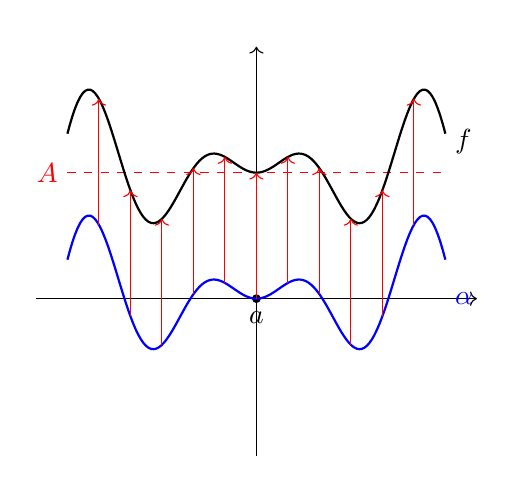
\begin{tikzpicture}[scale=0.8]
          % Coordinate axes
          \draw[->] (-3.5,0) -- (3.5,0) node[right] {};
          \draw[->] (0,-2.5) -- (0,4) node[above] {};
          
          % Point a on x-axis
          \node at (0,-0.3) {$a$};
          \fill (0,0) circle (0.07);
          
          % Blue function (alpha): x*sin(x)
          \draw[blue, thick, domain=-3:3, samples=150] 
            plot (\x, {0.5*\x*sin(3*\x r)});
          
          % Blue alpha label without arrow
          \node[blue, right] at (3,0) {$\alpha$};
          
          % Red horizontal line for A
          \draw[red, dashed] (-3,2) -- (3,2);
          \node[red, left] at (-3,2) {$A$};
          
          % Black function (f): x*sin(x) + 2
          \draw[black, thick, domain=-3:3, samples=150] 
            plot (\x, {0.5*\x*sin(3*\x r) + 2});
          
          % Black f label without arrow
          \node[black, right] at (3,2.5) {$f$};
          
          % Red vertical arrows connecting blue function to red line
          \foreach \x in {-2.5, -2.0, -1.5, -1.0, -0.5, 0, 0.5, 1.0, 1.5, 2.0, 2.5}
          \draw[->, red] (\x, {0.5*\x*sin(3*\x r)}) -- (\x, {0.5*\x*sin(3*\x r) + 2});
      \end{tikzpicture}
      \caption{Shift of $f(x) = \frac{1}{2} x \sin(3x) + 2$.} 
      \label{fig:infinitesimal_shift_function}
    \end{figure}
  \end{theorem}

  Finally, we reiterate some limit theorems already stated for sequences, but now corresponding to functions. Interpreting the function limit as the Cauchy sequence definition of limits renders the proofs of these theorems trivial. 

  \begin{theorem}[Bounds on Limits of Functions]
    If the functions $f, g: E \rightarrow \mathbb{R}$ are such that
    \begin{equation}
      \lim_{x\rightarrow a} f(x) = A < B = \lim_{x \rightarrow a} g(x)
    \end{equation}
    then there exists a deleted neighborhood $U_\delta (a)$ in $E$ at each point of which $f(x) < g(x)$. 
  \end{theorem}

  \begin{theorem}[Squeeze Theorem for Limits of Functions]
    Given the functions $f, g, h: E \subset \mathbb{R} \longrightarrow \mathbb{R}$ such that
    \begin{equation}
      f(x) \leq g(x) \leq h(x) \text{ for all } x \in E
    \end{equation}
    then, 
    \begin{equation}
      \lim_{x \rightarrow a} f(x) = \lim_{x \rightarrow a} h(x) = C \implies \lim_{x \rightarrow a} g(x) = C
    \end{equation}
  \end{theorem}

\subsection{Asymptotic Behavior of Functions}

    \begin{definition}[Little-O Notation]
      The function $f: E \longrightarrow \mathbb{R}$ is said to be \textbf{infinitesimal compared with the function $g: E \longrightarrow \mathbb{R}$} as $x \rightarrow a$, written (by abuse of notation) $f = o(g)$ as $x \rightarrow a$, if 
      \[\lim_{x \rightarrow a} \frac{f(x)}{g(x)} = 1\]
      or in other words, if $f/g$ is an infinitesimal function as $x \rightarrow a$. Therefore, $f = o(1)$ as $x \rightarrow a$ means that $f$ is infinitesimal as $x \rightarrow a$. \footnote{Note that writing $f = o(g)$ is again, an abuse of notation. $f = o(g)$ is really a shorthand way of writing that $f$ is in the class of functions that is infinitesimal compared with the function $g$.}
    \end{definition}

    Intuitively, $f = o(g)$ means that the ratio between $f(x)$ and $g(x)$ will tend to infinity as $x \rightarrow a$ (this does not mean that $f$ will be infinitely greater than $g$, however!). 

    \begin{example}[Linear vs Quadratic]
      For example, looking at the two functions $f(x) = x^2$ and $g(x) = x$, we have 
      \begin{enumerate}
        \item $x^2 = o(x)$ as $x \rightarrow 0$ (since $\frac{x^2}{x} = x$ is infinitesimal as $x \rightarrow 0$)
        \item $x = o(x^2)$ as $x \rightarrow \infty$ (since $\frac{x}{x^2} = \frac{1}{x}$ is infinitesimal as $x \rightarrow \infty$)
      \end{enumerate}
      We can visualize $g/f (x)$ tending to infinity within a neighborhood of $0$ and $f/g (x)$ tending to infinity within a neighborhood of $\infty$. 
      
      \begin{figure}[H]
        \centering 
        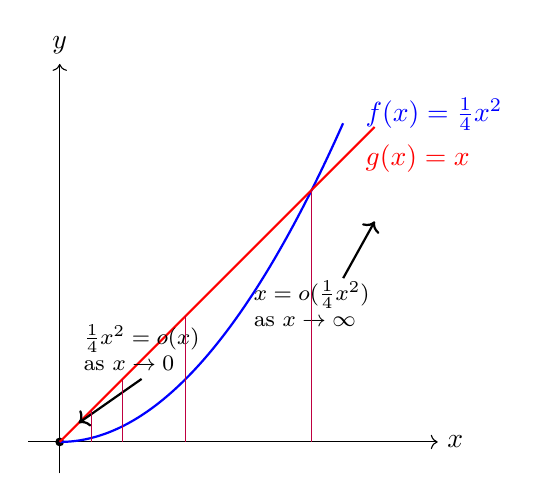
\begin{tikzpicture}[scale=0.8]
            % Coordinate axes
            \draw[->] (-0.5,0) -- (6,0) node[right] {$x$};
            \draw[->] (0,-0.5) -- (0,6) node[above] {$y$};
            
            % Origin point
            \fill (0,0) circle (0.07);
            
            % Blue parabola: f(x) = 1/4 * x^2
            \draw[blue, thick, domain=0:4.5, samples=100] 
              plot (\x, {0.25*\x*\x});
            
            % Red linear function: g(x) = x
            \draw[red, thick, domain=0:5, samples=2] 
              plot (\x, {\x});
            
            % Function labels
            \node[blue, right] at (4.7,5.2) {$f(x)=\frac{1}{4}x^2$};
            \node[red, right] at (4.7,4.5) {$g(x)=x$};
            
            % Asymptotic behavior annotations
            \node[align=left, font=\footnotesize] at (1.3,1.5) {$\frac{1}{4}x^2=o(x)$\\as $x\to 0$};
            \draw[->, thick] (1.3,1) -- (0.3,0.3);
            
            \node[align=left, font=\footnotesize] at (4,2.2) {$x=o(\frac{1}{4}x^2)$\\as $x\to\infty$};
            \draw[->, thick] (4.5,2.6) -- (5,3.5);
            
            % Vertical comparison lines
            \draw[purple, thin] (0.5,0) -- (0.5,0.5);
            \draw[purple, thin] (0.5,0) -- (0.5,0.0625);
            
            \draw[purple, thin] (1,0) -- (1,1);
            \draw[purple, thin] (1,0) -- (1,0.25);
            
            \draw[purple, thin] (2,0) -- (2,2);
            \draw[purple, thin] (2,0) -- (2,1);
            
            \draw[purple, thin] (4,0) -- (4,4);
            \draw[purple, thin] (4,0) -- (4,4);
        \end{tikzpicture}
        \caption{} 
        \label{fig:quadratic_vs_linear}
      \end{figure}
    \end{example}

    \begin{definition}[Orders of Infinitesimals, Infinities]
      If $f = o(g)$ and $g$ is infinitesimal as $x \rightarrow a$, then $f$ is an \textbf{infinitesimal of higher order than $g$ as $x \rightarrow a$}. Furthermore, if $f$ and $g$ are infinite functions as $x\rightarrow a$ and $f = o(g)$ as $x \rightarrow a$, then $g$ is a \textbf{higher order infinity than $f$ as $x \rightarrow a$}. 
    \end{definition}

    \begin{definition}[Big-O Notation]
      By abuse of notation, $f = O(g)$ as $x \rightarrow a$ means that 
      \begin{equation}
        \lim_{x \rightarrow a} \frac{f(x)}{g(x)} = \infty
      \end{equation}
      or in other words, $f/g$ is ultimately bounded as $x \rightarrow a$. In particular, $f = O(1)$ as $x \rightarrow a$ means that $f$ is bounded within a certain neighborhood $U(a)$ of $a$. 
    \end{definition}

    \begin{definition}[Functions of Same Order]
      The functions $f$ and $g$ are of the same over as $x \rightarrow a$, written 
      \begin{equation}
        f \asymp g \text{ as } x \rightarrow a
      \end{equation}
      if $f = O(g)$ and $g = O(f)$ as $x \rightarrow a$. Intuitively, this means that the ratio between $f$ and $g$ within some deleted neighborhood of $a$ is finite. 

      Note that the condition that $f$ and $g$ be of the same order as $x \rightarrow a$ is (by definition of ultimately bounded functions) equivalent to the condition that there exist $c_1, c_2 > 0$ and an open neighborhood $U (a)$ such that the relations
      \begin{equation}
        c_1 |g(x)| \leq |f(x)| \leq c_2 |g(x)|
      \end{equation}
      is true for $x \in U(a)$. 
    \end{definition}

    \begin{definition}[Asymptotic Equivalence of Functions]
      For functions $f$ and $g$, if 
      \begin{equation}
        \lim_{x \rightarrow a} \frac{f(x)}{g(x)} = 1
      \end{equation}
      we say that \textbf{$f$ behaves asymptotically like $g$ as $x \rightarrow a$}, or that \textbf{$f$ is equivalent to $g$ as $x \rightarrow a$}, written 
      \begin{equation}
        f \sim g \text{ as } x \rightarrow a
      \end{equation}
      Moreover, $\sim$ is an equivalence relation, which means that
      \begin{enumerate}
        \item $f \sim f$ as $x \rightarrow a$
        \item $f \sim g$ as $x \rightarrow a \implies$ $g \sim f$ as $x \rightarrow a$
        \item $f \sim g$ and $g \sim h$ as $x \rightarrow a \implies f \sim h$ as $x \rightarrow a$
      \end{enumerate}
    \end{definition}

    We list a few examples in order to develop some sort of visual intuition for when two functions are asymptotically equivalent. 

    \begin{example}[Both Converges at Finite Value to Nonzero Finite Value]
      If $f(a) = g(a) \neq 0$, then $f \sim g$ trivially since the ratio of $f$ and $g$ converges to $1$ within a neighborhood of $a$. 

      \begin{figure}[H]
        \centering 
        \begin{tikzpicture}[scale=1.2]
          % Coordinate axes
          \draw[->] (-3,0) -- (3,0) node[right] {$x$};
          \draw[->] (0,-1) -- (0,3) node[above] {$y$};
          
          % Blue curve - single smooth wave with no other intersections
          \draw[blue, thick, smooth] 
            plot[domain=-3:3, samples=50] (\x, {1.5 + 0.8*sin(\x*40)});
          
          % Red curve - continuous rise with no other intersections
          \draw[red, thick, smooth] 
            plot[domain=-2:3, samples=50] (\x, {0.2*\x*\x - 0.6*\x + 1});
          
          % Point of intersection
          \fill (-0.4,1.25) circle (0.05);
          \node[above] at (-0.4,1.25) {$a$};
        \end{tikzpicture}
        \caption{} 
      \end{figure}
    \end{example}

    \begin{example}[Both Converges at Finite Value to $0$]
      When $f(a) = g(a) = 0$, it may be $f$ may be equivalent to $g$ or one function may be infinitesimally smaller than the other. 

      \begin{figure}[H]
        \centering
        \begin{subfigure}[b]{0.48\textwidth}
          \centering
          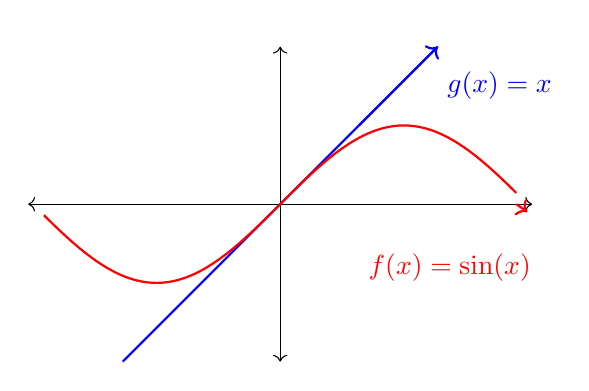
\begin{tikzpicture}[scale=1.0]
            % Coordinate axes
            \draw[<->] (-3.2,0) -- (3.2,0) node[right] {};
            \draw[<->] (0,-2) -- (0,2) node[above] {};
            
            % Blue line g(x) = x with restricted domain
            \draw[blue, thick] (-2,-2) -- (2,2);
            \node[blue, right] at (2,1.5) {$g(x)=x$};
            
            % Red sine curve f(x) = sin(x)
            \draw[red, thick, domain=-3:3, samples=100] 
              plot (\x, {sin(\x r)});
            \node[red, right] at (1,-0.8) {$f(x)=\sin(x)$};
            
            % Direction arrows
            \draw[blue, ->, thick] (1,1) -- (2,2);
            \draw[red, ->, thick] (3,0) -- (3.14,-0.1);
          \end{tikzpicture}
          \caption{When $f(x) = \sin{x}$ and $g(x) = x$, then $f \sim g$ since we see that $\lim_{x \rightarrow 0} \frac{\sin{x}}{x} = 1$, and so $\sin{x} \sim x$ as $x \rightarrow 1$. }
        \end{subfigure}
        \hfill 
        \begin{subfigure}[b]{0.48\textwidth}
          \centering
          \begin{tikzpicture}[scale=0.8]
            % Coordinate axes
            \draw[<->] (-3.5,0) -- (3.5,0) node[right] {};
            \draw[<->] (0,-3) -- (0,3) node[above] {};
            
            % Red parabola f(x) = x^2
            \draw[red, thick, domain=-2.5:2.5, samples=50] 
              plot (\x, {\x*\x*0.2});
            \node[red, right] at (2.5,2.5) {$f(x)=x^2$};
            
            % Blue cubic g(x) = x^3
            \draw[blue, thick, domain=-2.3:2.3, samples=50] 
              plot (\x, {\x*\x*\x*0.2});
            \node[blue, right] at (2.5,2) {$g(x)=x^3$};
          \end{tikzpicture}
          \caption{When $f(x) = x^2$ and $g(x) = x^3$, then $\lim_{x \rightarrow 0} \frac{x^3}{x^2} = 0$, and so $x^3 \not\sim x^2$. In fact, $x^3 = o(x^2)$. }
        \end{subfigure}

        \begin{subfigure}[b]{0.48\textwidth}
          \centering
          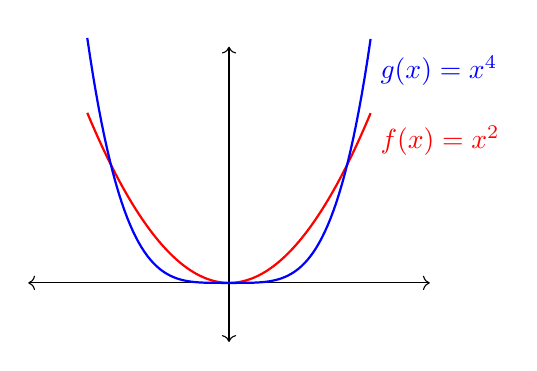
\begin{tikzpicture}[scale=1.5]
            % Coordinate axes
            \draw[<->] (-1.7,0) -- (1.7,0) node[right] {};
            \draw[<->] (0,-0.5) -- (0,2) node[above] {};
            
            % Red parabola f(x) = x^2
            \draw[red, thick, domain=-1.2:1.2, samples=100] 
              plot (\x, {\x*\x});
            \node[red, right] at (1.2,1.2) {$f(x)=x^2$};
            
            % Blue g(x) = x^4
            \draw[blue, thick, domain=-1.2:1.2, samples=100] 
              plot (\x, {\x*\x*\x*\x});
            \node[blue, right] at (1.2,1.8) {$g(x)=x^4$};
          \end{tikzpicture}
          \caption{When $f(x) = x^2$ and $g(x) = x^4$, then  $\lim_{x \rightarrow 0} \frac{x^4}{x^2} = 0$, and so $x^4 \not\sim x^2$. In fact, $x^4 = o(x^2)$. }
        \end{subfigure}
        \hfill 
        \begin{subfigure}[b]{0.48\textwidth}
          \centering
          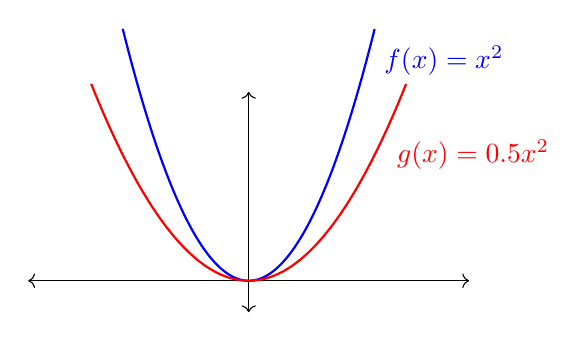
\begin{tikzpicture}[scale=0.8]
            % Coordinate axes
            \draw[<->] (-3.5,0) -- (3.5,0) node[right] {};
            \draw[<->] (0,-0.5) -- (0,3) node[above] {};
            
            % Blue parabola f(x) = x^2
            \draw[blue, thick, domain=-2:2, samples=100] 
              plot (\x, {\x*\x});
            \node[blue, right] at (2,3.5) {$f(x)=x^2$};
            
            % Red parabola g(x) = 0.5x^2
            \draw[red, thick, domain=-2.5:2.5, samples=100] 
              plot (\x, {0.5*\x*\x});
            \node[red, right] at (2.2,2) {$g(x)=0.5x^2$};
          \end{tikzpicture}
          \caption{When $f(x), g(x) = x^2, 0.5x^2$, then $\lim_{x \rightarrow 0} \frac{0.5x^2}{x^2} = \frac{1}{2}$. So $0.5x^2 \not\sim x^2$. }
        \end{subfigure}
        \caption{Examples of different scenarios.}
        \label{fig:converge_to_finite_value_0}
      \end{figure}
    \end{example}

    \begin{example}[Analyzing at Infinity]
      When analyzing the behavior of functions as $x \rightarrow \infty$, we can picture the two graphs of $f$ and $g$ on the plane and "zoom out" to see if the ratio of the values converge to $1$. This would mean that as $x \rightarrow \infty$, we should see the graphs overlapping more and more. 

      \begin{figure}[H]
        \centering
        \begin{subfigure}[b]{0.48\textwidth}
          \centering
          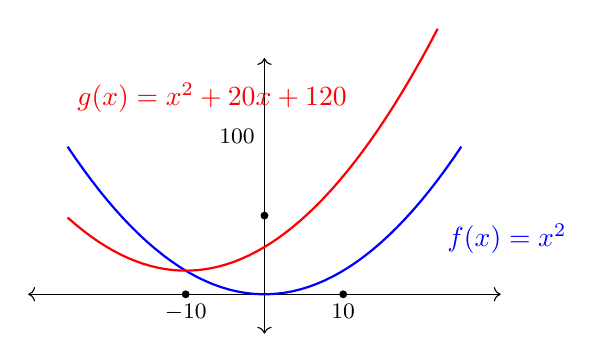
\begin{tikzpicture}[scale=1]
              % Coordinate axes
              \draw[<->] (-3,0) -- (3,0) node[right] {};
              \draw[<->] (0,-0.5) -- (0,3) node[above] {};
              
              % Blue parabola f(x) = x^2
              \draw[blue, thick, domain=-2.5:2.5, samples=50] 
                plot (\x, {0.3 * \x*\x});
              \node[blue, right] at (2.2,0.7) {$f(x)=x^2$};
              
              % Red parabola g(x) = x^2 + 10x + 100
              \draw[red, thick, domain=-2.5:2.2, samples=50] 
                plot (\x, {0.3 * (\x*\x + 2*\x + 2)});
              \node[red, right] at (-2.5,2.5) {$g(x)=x^2+20x+120$};
              
              % Key points on x-axis with labels
              \fill (-1,0) circle (0.05);
              \node[below, font=\footnotesize] at (-1,0) {$-10$};
              
              \fill (1,0) circle (0.05);
              \node[below, font=\footnotesize] at (1,0) {$10$};
              
              \fill (0,1) circle (0.05);
              \node[left, font=\footnotesize] at (0,2) {$100$};
          \end{tikzpicture}
          \caption{Comparison of $f(x)=x^2$ and $g(x)=x^2+10x+100$}
          \label{fig:shifted-quadratic}
        \end{subfigure}
        \hfill 
        \begin{subfigure}[b]{0.48\textwidth}
          \centering
          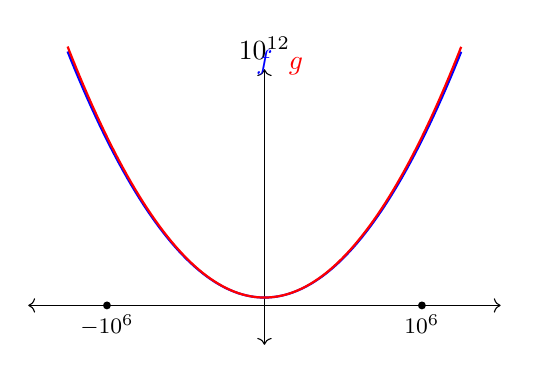
\begin{tikzpicture}[scale=1]
              % Coordinate axes
              \draw[<->] (-3,0) -- (3,0) node[right] {};
              \draw[<->] (0,-0.5) -- (0,3) node[above] {$10^{12}$};
              
              % Functions with nearly identical behavior
              \draw[blue, thick, domain=-2.5:2.5, samples=100] 
                plot (\x, {0.1 + 0.5*\x*\x});
              \node[blue, above] at (0,2.8) {$f$};
              
              % Red function slightly above blue
              \draw[red, thick, domain=-2.5:2.5, samples=100] 
                plot (\x, {0.1 + 0.51*\x*\x});
              \node[red, above] at (0.4,2.8) {$g$};
              
              % Key points on x-axis with labels
              \fill (-2,0) circle (0.05);
              \node[below, font=\footnotesize] at (-2,0) {$-10^6$};
              
              \fill (2,0) circle (0.05);
              \node[below, font=\footnotesize] at (2,0) {$10^6$};
          \end{tikzpicture}
          \caption{Asymptotic behavior with $g/f \approx 1$}
          \label{fig:asymptotic}
        \end{subfigure}
        \caption{taking $f(x) = x^2$ and $g(x) = x^2 + 10x + 100$, we can see that the discrepancy is high around a neighborhood of $x = 0$. But as $x \rightarrow +\infty$, we get $\lim_{x \rightarrow + \infty} \frac{x^2 + 10x + 100}{x^2} = 1$, and so the graphs look like they are overlapping. Notice that even though the absolute difference $|(x^2 + 10x + 100) - x^2| = |10x + 100|$ tends to infinity, this difference increases infinitesimally compared to $f$ and $g$. }
        \label{fig:function-ratios}
      \end{figure}
    \end{example}

    From this, we can see that if $f \sim g$ as $x \rightarrow a$, then their difference 
    \begin{equation}
      f - g = o(g) = o(f)
    \end{equation}
    That is, $(f-g)(x)$ is infinitesimal compared to $g$ or $f$ (doesn't matter which one we compare it to). This leads to our next section, where we formalize this concept with absolute and relative errors. 

  \subsubsection{Approximations of Functions}

    It is useful to note that since the relation $\lim_{x \rightarrow a} \gamma(x) = 1$ is equivalent to 
    \begin{equation}
      \gamma (x) = 1 + \alpha(x), \text{ where } \lim_{x \rightarrow a} \alpha(x) = 0
    \end{equation}
    the relation $f \sim g$ as $x\rightarrow a$ is equivalent to saying that
    \begin{equation}
      \frac{f(x)}{g(x)} = \gamma(x), \text{ where } \lim_{x \rightarrow a} \gamma(x) = 1
    \end{equation}
    which implies 
    \begin{equation}
      f(x) = g(x) + \alpha(x) g(x) = g(x) + o(g(x)) \text{ as } x \rightarrow a
    \end{equation}
    or, symmetrically, 
    \begin{equation}
      g(x) = f(x) + \alpha(x) f(x) = f(x) + o(f(x)) \text{ as } x \rightarrow a
    \end{equation}
    This means that $f$ can be exactly represented by another function $g$, plus another (error) function $o(g(x))$ that is infinitesimal compared to $g$. 

    \begin{figure}[H]
      \centering
      \begin{subfigure}[b]{0.48\textwidth}
        \centering
        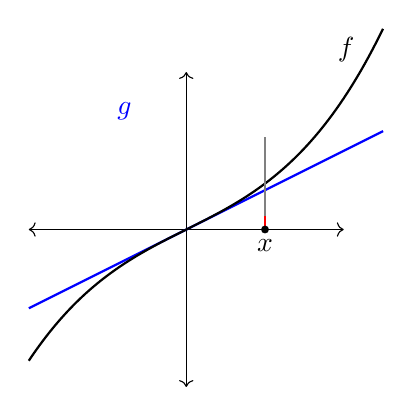
\begin{tikzpicture}[scale=1]
            % Coordinate axes
            \draw[<->] (-2,0) -- (2,0) node[right] {};
            \draw[<->] (0,-2) -- (0,2) node[above] {};
            
            % Blue line g(x) = x
            \draw[blue, thick, domain=-2:2.5, samples=2] 
              plot (\x, {\x * 0.5});
            \node[blue, right] at (-1,1.5) {$g$};
            
            % Black cubic f(x) = x^3/6 + x
            \draw[black, thick, domain=-2:2.5, samples=100] 
              plot (\x, {((\x*\x*\x)/6 + \x) * 0.5});
            \node[black, above right] at (1.8,2) {$f$};
            
            % Vertical line at a point
            \draw[gray, thin] (1,0) -- (1,1);
            \draw[gray, thin] (1,1) -- (1,1.17);
            \draw[red, thin] (1,0) -- (1,0.17);
            
            % Point label
            \fill (1,0) circle (0.05);
            \node[below] at (1,0) {$x$};
        \end{tikzpicture}
        \caption{Functions $f$, $g$, and their difference}
        \label{fig:function-diff}
      \end{subfigure}
      \hfill 
      \begin{subfigure}[b]{0.48\textwidth}
        \centering
        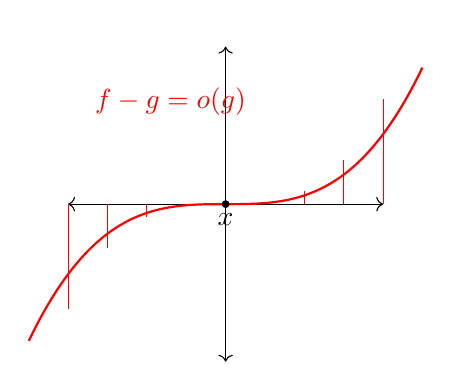
\begin{tikzpicture}[scale=1]
            % Coordinate axes
            \draw[<->] (-2,0) -- (2,0) node[right] {};
            \draw[<->] (0,-2) -- (0,2) node[above] {};
            
            % Red function f-g = x^3/6
            \draw[red, thick, domain=-2.5:2.5, samples=100] 
              plot (\x, {(\x*\x*\x)/9});
            \node[red, above] at (-0.7,1) {$f-g = o(g)$};
            
            % Vertical lines showing difference
            \foreach \x in {-2, -1.5, -1, -0.5, 0.5, 1, 1.5, 2} {
                \draw[red, thin] (\x,0) -- (\x,{(\x*\x*\x)/6});
            }
            
            % Point at origin
            \fill (0,0) circle (0.05);
            \node[below] at (0,0) {$x$};
        \end{tikzpicture}
        \caption{Behavior of $f-g$ (little-o of $g$)}
        \label{fig:little-o}
      \end{subfigure}
      \caption{Visualization of asymptotic behavior where $f-g = o(g)$}
      \label{fig:asymptotic-behavior}
    \end{figure}

    Note that it is not a sufficient condition that the error function be infinitesimal! The error function $f-g$ must be infinitesimal \textit{compared to $g$}! This tells us that not only does the error function decrease infinitesimally, but also is infinitesimal compared to the approximation function we already have, which is in general a much stronger claim. This representation of certain types functions will provide the foundation for differential calculus when we talk about "good" approximations for a function. 


    \begin{definition}[Relative Error]
      Since $f \sim g$ as $x \rightarrow a$ means that 
      \begin{equation}
        f(x) = g(x) + \alpha(x) g(x) = g(x) + o(g(x))
      \end{equation}
      we can define the \textbf{relative error} of $g$ as an approximation of $f$ to be
      \begin{equation}
        |\alpha(x)| = \bigg| \frac{f(x) - g(x)}{g(x)} \bigg|
      \end{equation}
      Clearly, since $f \sim g$, the relative error must be infinitesimal as $x \rightarrow a$. 
    \end{definition}

    We use the following lemma to check whether two functions are asymptotically equivalent. 
    \begin{lemma}
      $f \sim g$ as $x \rightarrow a$ if and only if the relative error of $g$ is infinitesimal as $x \rightarrow a$. 
    \end{lemma}

    \begin{example}
      We claim that 
      \begin{equation}
        x^2 + x = \bigg(1 + \frac{1}{x} \bigg) x^2 \sim x^2 \text{ as } x \rightarrow \infty
      \end{equation}
      We see that the absolute error of this approximation $|(x^2 + x) - x^2| = |x|$ tends to infinity, but the relative error $\frac{|x|}{x^2} = \frac{1}{|x|} \rightarrow 0$ as $x \rightarrow \infty$. 
    \end{example}

    \begin{theorem}[Prime Number Theorem]
      Let $\pi(x)$ be the number of prime numbers strictly less than $x$. Then $\pi \sim \frac{x}{\ln{x}}$ as $x\rightarrow + \infty$, or more precisely, 
      \begin{equation}
        \pi(x) = \frac{x}{\ln{x}} + o \bigg( \frac{x}{\ln{x}}\bigg) \text{ as } x \rightarrow +\infty
      \end{equation}
    \end{theorem}

    \begin{example}
      It is a fact that $\lim_{x\rightarrow 0} \frac{sin{x}}{x} = 1$, so we have $\sin{x} \sim x$ as $x \rightarrow 0$. So,
      \begin{equation}
        \sin{x} = x + o(x) \text{ as } x \rightarrow 0
      \end{equation}
    \end{example}

    The following theorem proves useful when computing limits. 

    \begin{theorem}
      If $f \sim \Tilde{f}$ as $x \rightarrow a$, then 
      \begin{equation}
        \lim_{x \rightarrow a} f(x) g(x) = \lim_{x \rightarrow a} \Tilde{f}(x) g(x)
      \end{equation}
      provided one of these limits exist. 
    \end{theorem}

    \begin{theorem}[Properties of $o(g)$ and $O(g)$ Functions]
      For $x \rightarrow a$, 
      \begin{enumerate}
        \item $o(f) + o(f) = o(f)$
        \item $o(f)$ is also $O(f)$
        \item $o(f) + O(f) = O(f)$
        \item $O(f) + O(f) = O(f)$
        \item If $g(x) \not\equiv 0$, then 
        \begin{equation}
          \frac{o(f(x))}{g(x)} = o \bigg( \frac{f(x)}{g(x)} \bigg), \text{ and } \frac{O(f(x))}{g(x)} = O \bigg( \frac{f(x)}{g(x)} \bigg)
        \end{equation}
      \end{enumerate}
    \end{theorem}

\subsection{Continuous Functions}

  \begin{definition}[Continuity of a Function]
    A function $f$ is \textbf{continuous at point $a$} if for any neighborhood $V\big(f(a)\big)$ of $f(a)$, there is a neighborhood $U(a)$ of $a$ whose image under the mapping $f$ is contained in $V\big( f(a)\big)$. 

    Generalizing this, we say that a function is \textbf{(globally) continuous} if the preimage of every neighborhood in its codomain is an open set in its domain. 
  \end{definition}

  \begin{lemma}[Existence of Limits of Continuous Functions]
    $f: E \longrightarrow \mathbb{R}$ is continuous at $a \in E$, where $a$ is a limit point of $E$ if and only if 
    \begin{equation}
      \lim_{x \rightarrow a} f(x) = f(a)
    \end{equation}
  \end{lemma}
  \begin{proof}
    The limit equaling $f(a)$ means that, by definition, for any arbitrarily small deleted neighborhood of $f(a)$, denoted $U_{f(a)} \setminus f(a)$, its preimage will be an open neighborhood of $a$, which itself will contain an open set. 
  \end{proof}

  This also means that we can use the Cauchy limit definition to defined continuity of a function at a point. That is, for any sequence $\{a_n\}$ of point in codomain $E$ which converges to point $a$, the function $f$ is continuous at $a$ if the corresponding sequence $\{f(a_n)\}$ converges to $f(a)$.

  \begin{theorem}
    This means that the continuous functions commute with the operation of passing to the limit at a point. 
    \begin{equation}
      \lim_{x \rightarrow a} f(x) = f\Big( \lim_{x \rightarrow a} x \Big)
    \end{equation}
  \end{theorem}

  \begin{lemma}[Properties of Continuous Functions]
    Let $f: \mathbb{R}^n \longrightarrow \mathbb{R}^m, \; g: \mathbb{R}^m \longrightarrow \mathbb{R}^p$ with $c \in \mathbb{R}$. 
    \begin{enumerate}
      \item $f$ continuous at $x_0 \implies$ $c f$ continous at $x_0$. 
      \item $f, g$ continuous at $x_0 \implies f + g$ continuous at $x_0$. 
      \item Let $m = 1$. $f, g$ continuous at $x_0 \implies f g$ continuous at $x_0$. 
      \item $f$ continuous at $x_0$ and $f(x) \neq 0 \forall x \in \mathbb{R}^n \implies 1 / f$ continuous at $x_0$. 
      \item If $f(x) = \big( f_1(x), f_2(x), ..., f_n(x) \big)$ coordinate-wise, then 
      \begin{equation}
        f \text{ continuous at } x_0 \iff f_1, f_2, ..., f_m \text{ continuous  at } x_0
      \end{equation}
      \item $f$ continuous at $x_0$ and $g$ continuous at $y_0 = f(x_0) \implies g \circ f$ continuous at $x_0$. 
    \end{enumerate}
  \end{lemma}
  \begin{proof}
    This is an immediate result of the equivalence of a function being continuous at point $a$ and its limit at point $a$ existing. 
  \end{proof}

  \begin{theorem}[Local Properties of Continuous Functions]
    Let $f: E \longrightarrow \mathbb{R}$ be a function that is continuous at the point $a \in E$. Then, 
    \begin{enumerate}
      \item $f$ is bounded in some neighborhood $U(a)$. 
      \item If $f(a) \neq 0$, then in some neighborhood $U(a)$ all the values of the function have the same sign as $f(a)$. 
      \item If the function $g: U(a) \subset E \longrightarrow \mathbb{R}$ is defined in some neighborhood of $a$ and is continuous at $a$, then the following functions 
      \begin{align*}
        & (f + g) (x) \\
        & (f \cdot g) (x) \\
        & \bigg( \frac{f}{g} \bigg) \big( x \big) \text{ where } g(a) \neq 0
      \end{align*}
      are also defined in $U(a)$ and continuous at $a$. 
      \item If the function $g: Y \longrightarrow \mathbb{R}$ is continuous at a point $b \in Y$ and $f$ is such that $f: E \longrightarrow Y$, $f(a) = b$, and $f$ is continuous at $a$, then the composite function 
      \[g \circ f: E \longrightarrow \mathbb{R}\]
      is defined on $E$ and continuous at $a$. This is easy to see because given the open neighborhood of $g(b)$, we know for a fact that $U_\delta (a)$ maps completely into $U_\epsilon (b)$, and that $U_\epsilon (b)$ maps completely into $U_\kappa (g(b))$ and so the composition of these mappings must mean that $U_\delta (a)$ maps completely into $U_\kappa (g(b))$. 
    \end{enumerate}
  \end{theorem}

  \begin{example}
    An algebraic polynomial 
    \begin{equation}
      P(x) = a_0 x^n + a_1 x^{n-1} + a_2 x^{n-2} + \ldots + a_{n-1} x + a_n
    \end{equation}
    is a continuous function on $\mathbb{R}$. Since $f(x) = x$ and $f(x) = c$ are continuous functions, by induction on $x$, we can multiply them together to find that $f(x) = x^n$ is continuous, which implies that $a x^n$ is continuous, which implies that the sums of these functions are also continuous. 
  \end{example}

  \subsubsection{Intermediate and Extreme Value Theorem}

    Unlike local properties, the global property of a function is a property involving the entire domain of definition of the function. 

    \begin{theorem}[Intermediate Value Theorem]
      If a function that is continuous on a closed interval assumes values with different signs at the endpoints of the interval, then there is a point in the interval where it assumes the value $0$. 
      \begin{center}
          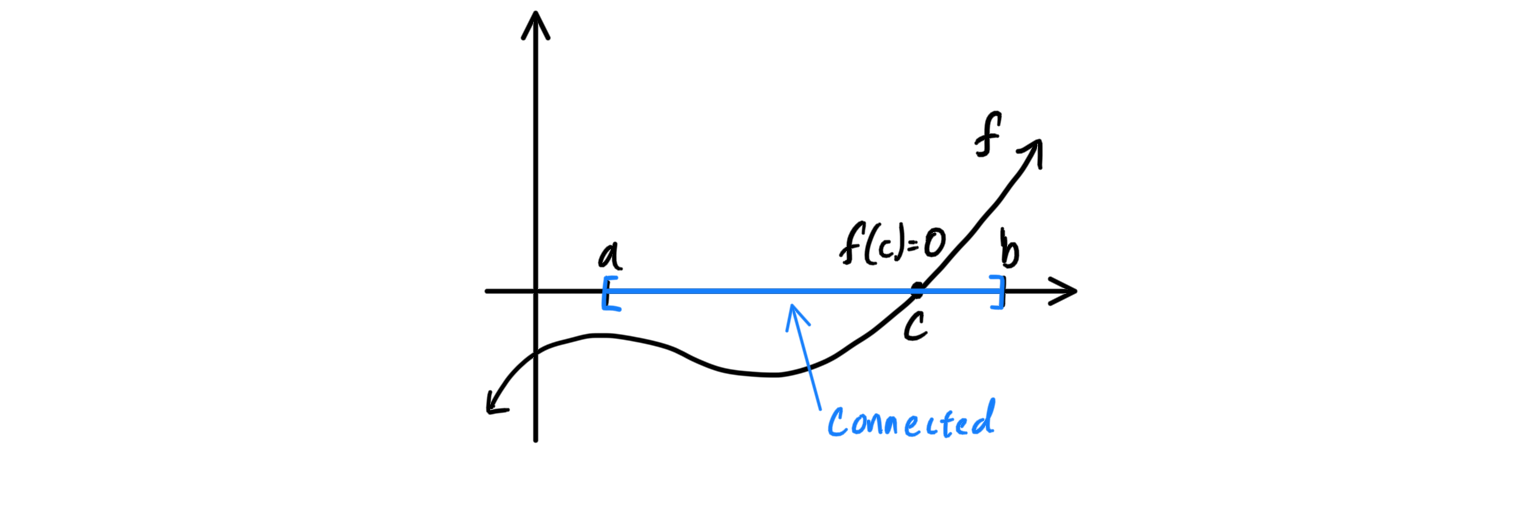
\includegraphics[scale=0.25]{img/IVT.PNG}
      \end{center}
    \end{theorem}
    \begin{proof}

    \end{proof}

    This following proof provides a very simple algorithm for finding the zero of the equation $f(x) = 0$ on an interval whose endpoints has values with opposite signs. 
    Note that the colloquial description of the intermediate value theorem, that is is impossible to pass continuously from positive to negative values without assuming the value $0$ along the way), assumes more than they state. That is, this theorem is actually dependent on the domain of definition: that is is a closed interval, or more generally, that it is \textbf{connected}. 

    \begin{corollary}
      If a function $f$ is continuous on an open interval and assumes values $f(a) = A, f(b) = B$, then for any number $C \in (A, B)$, there is a point $c$ between $a$ and $b$ such that $f(c) = C$. 
      \begin{center}
        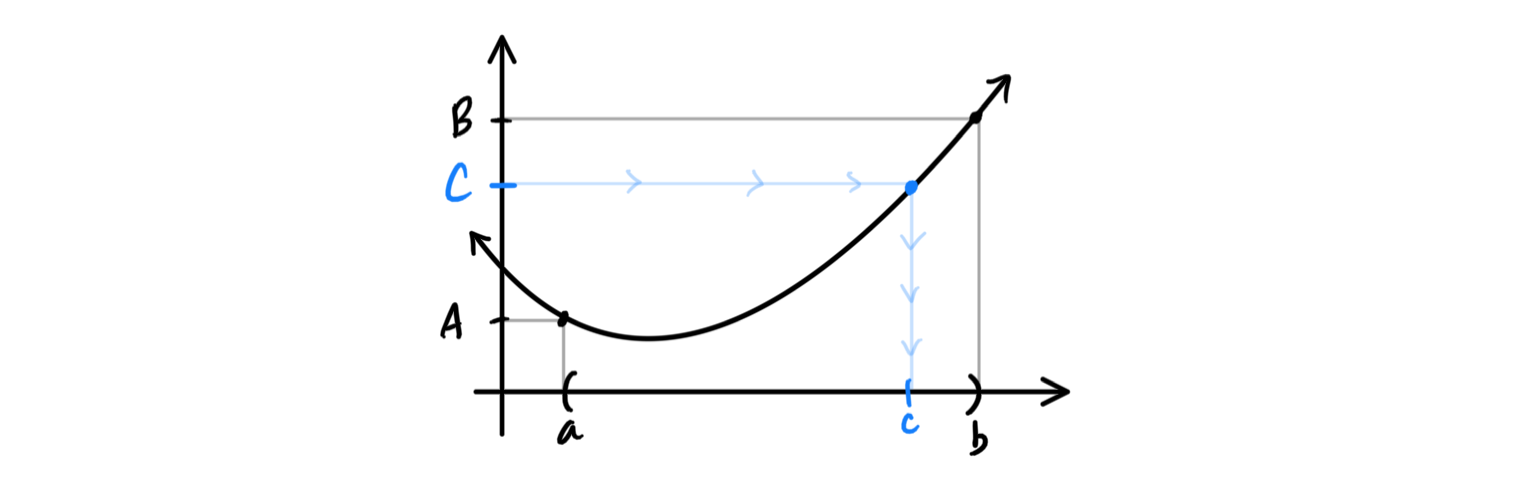
\includegraphics[scale=0.25]{img/Corollary_of_IVT.PNG}
      \end{center}
    \end{corollary}

    \begin{theorem}[Extreme Value Theorem]
      A continuous real-valued function over a compact set attains its maximum and minimum. 
    \end{theorem}

  \subsubsection{Inverse Function Theorem}

    We begin by introducing this intuitive lemma. 
    \begin{lemma}
      A continuous mapping $f: E \longrightarrow \mathbb{R}$ of a closed interval $E = [a,b]$ into $\mathbb{R}$ is injective if and only if the function $f$ is strictly monotonic on $[a,b]$. 

      Furthermore, every strictly monotonic function $f: X \subset \mathbb{R} \longrightarrow \mathbb{R}$ (for arbitrary $X$) has an inverse 
      \[f^{-1}: f(X) \subset \mathbb{R} \longrightarrow \mathbb{R}\]
      with the same kind of monotonicity on $f(X)$ that $f$ has on $X$. 
    \end{lemma}

    \begin{lemma}[Criterion for Continuity of a Monotonic Function]
      A monotonic function $f: E \longrightarrow \mathbb{R}$ defined on a closed interval $E = [a,b]$ is continuous if and only if its set of values $f(E)$ is the closed interval with endpoints $f(a)$ and $f(b)$. 

      Note that both conditions imply that there are no points of discontinuities in the graph of $f$. 
    \end{lemma}


    \begin{theorem}[Inverse Function Theorem]
    A function $f: X \longrightarrow \mathbb{R}$ that is strictly monotonic on a set $X \subset \mathbb{R}$ has an inverse $f^{-1}: Y \longrightarrow \mathbb{R}$ defined on the set $Y = f(X)$ of values of $f$. The function $f^{-1}: Y \longrightarrow \mathbb{R}$ is monotonic and has the same type of monotonicity on $Y$ that $f$ has on $X$. 
    \begin{center}
        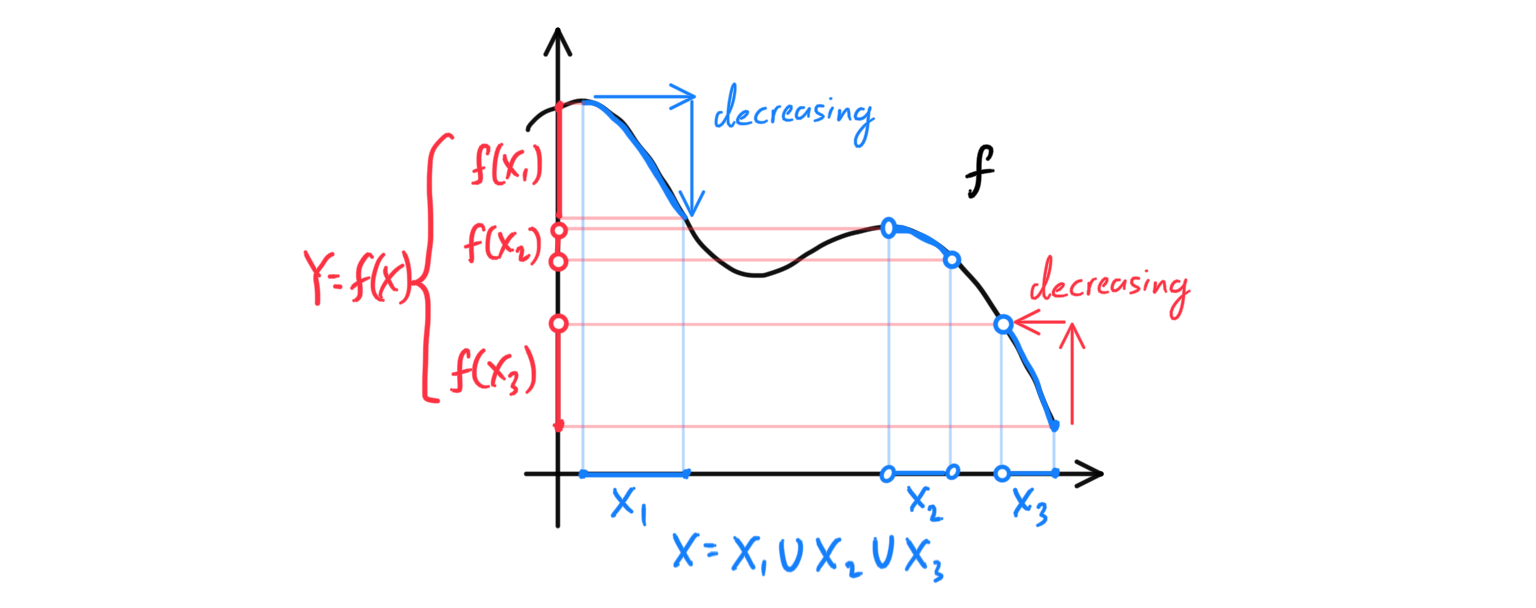
\includegraphics[scale=0.25]{img/Inverse_Function_Theorem_Analysis.PNG}
    \end{center}
    If in addition, $X$ is a closed interval $[a,b]$ and $f$ is continuous on $X$, then the set $Y = f(X)$ is the closed interval with endpoints $f(a)$ and $f(b)$ and the function $f^{-1}: Y \longrightarrow \mathbb{R}$ is continuous on it.
    \end{theorem}

    \begin{example}
      The function $f(x) = \sin{x}$ is increasing and continuous on the closed interval $\big[ -\frac{\pi}{2}, \frac{\pi}{2} \big]$. Hence, the restriction to the closed interval $\big[ -\frac{\pi}{2}, \frac{\pi}{2} \big]$ has an inverse $x = f^{-1}(y)$, which is denoted by 
      \[x = \arcsin{y}\]
      This function is defined on the closed interval $\big[- \sin\big(-\frac{\pi}{2}\big), \sin\big(-\frac{\pi}{2}\big) \big] = [-1,1]$ and increases continuously from $-\frac{\pi}{2}$ to $\frac{\pi}{2}$. 
      \begin{center}
          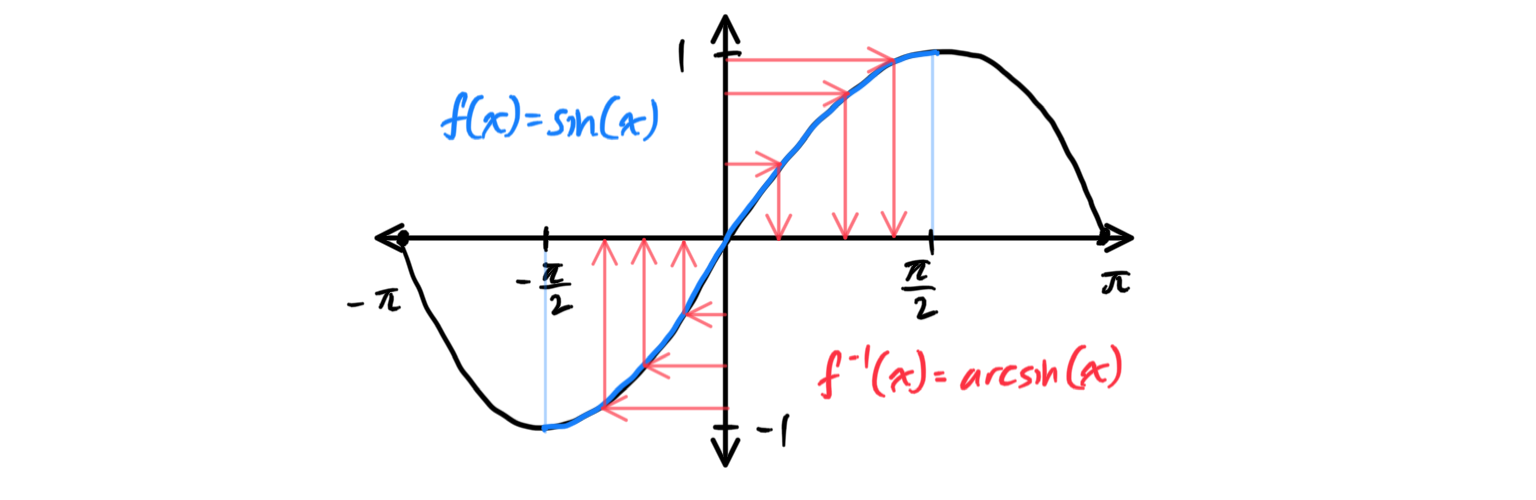
\includegraphics[scale=0.25]{img/Inverse_Function_Theorem_Sin.PNG}
      \end{center}
    \end{example}

\subsection{Uniform Continuity}

  Roughly speaking, a function $f$ is uniformly continuous if it is possible to guarantee that $f(x)$ and $f(y)$ be as close to each other as we please by requiring only that $x$ and $y$ be sufficiently close to each other. 

  \begin{definition}[Uniform Continuity]
    A function $f: E \longrightarrow \mathbb{R}$ is \textbf{uniformly continuous} on a set $E \subset \mathbb{R}$ if for every $\epsilon > 0$, there exists $\delta > 0$ such that 
    \begin{equation}
      \big| f(x_1) - f(x_2)\big| < \epsilon
    \end{equation}
    for all points $x_1, x_2 \in E$ such that $|x_1 - x_2| < \delta$. 

    Intuitively, uniform continuity says that given any two points $x, y$ in the domain where their distance is arbitrarily small ($\delta$ apart), we can guarantee that the distance between $f(x), f(y)$ is at maximum some arbitrarily small $\epsilon$. 

    The following visual shows the radical function $f(x) = \sqrt{x}$ defined on $\mathbb{R}^+$. We can see that it satisfies uniform continuity because the graph does not escape the top and/or bottom of the $\epsilon \times \delta$ window, no matter where the box is located on the graph. More strictly speaking, no matter what we set the $\epsilon$ (how long the box is), uniform continuity says that we can choose a sufficient $\delta$ (width of the box) such that the graph does not escape the top/bottom of the window no matter where the window is. 
    \begin{center}
        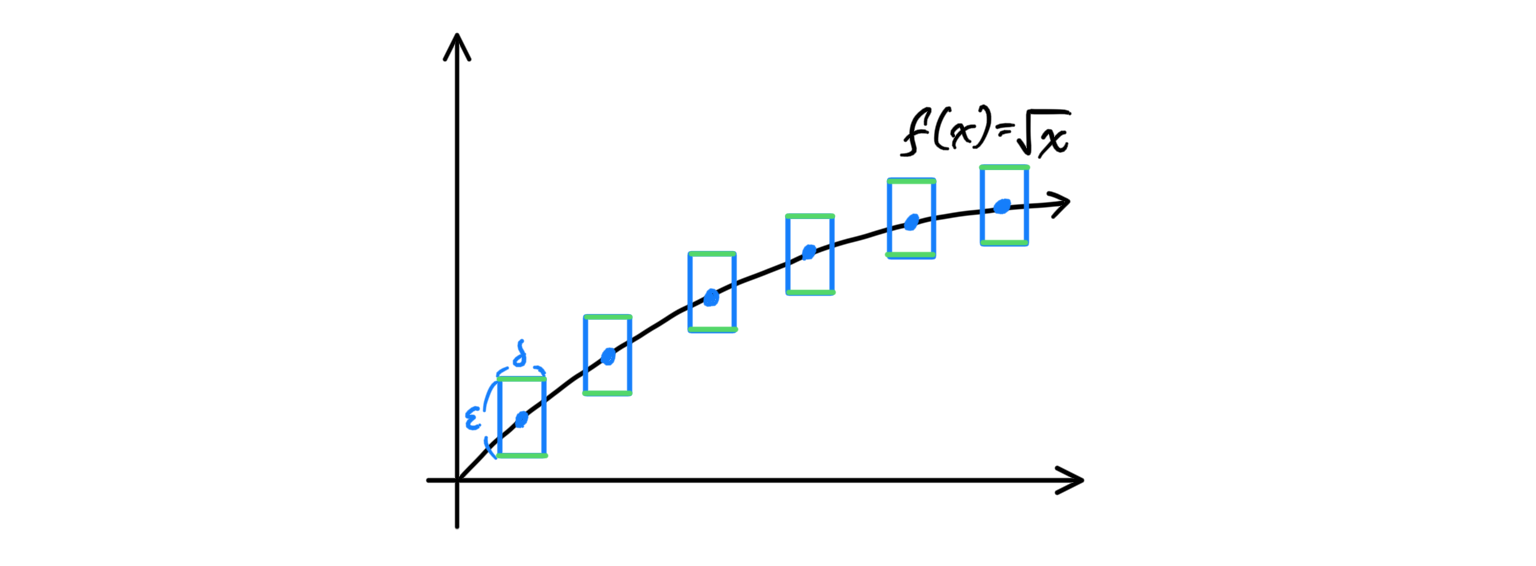
\includegraphics[scale=0.28]{img/Uniform_Continuity_Radical.PNG}
    \end{center}
    We can clearly see that the function $f(x) = 1/x$ is not uniformly continuous, since the graph escapes the $\epsilon \times \delta$ window at some point (marked in red). More strictly speaking, given any length $\epsilon$ of the window, we cannot create a thin-enough $\delta$ box that will contain the graph, since as $x \rightarrow 1$, the function becomes unbounded. 
    \begin{center}
        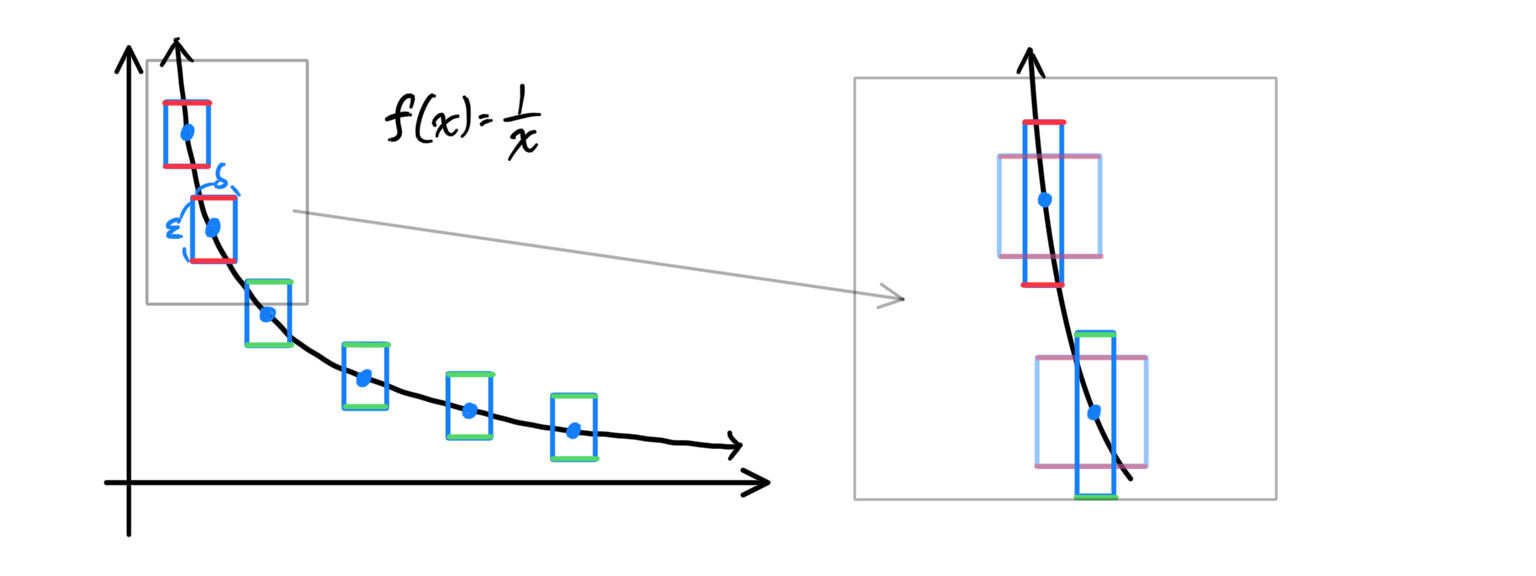
\includegraphics[scale=0.25]{img/Uniform_Continuity_Rational.PNG}
    \end{center}
    That is, arbitrarily thin boxes don't help when the slope is arbitrarily steep. 
  \end{definition}

  To compare uniform continuity with regular continuity, we can adapt this alternate (yet equivalent interpretation): Let there exist function $f: E \longrightarrow \mathbb{R}$. Given any $\epsilon>0$, we can choose a $\delta>0$ such that given any point $x \in E$ and $f(x)$, as long as a second point $y$ is $\delta$ away from $x$, then $f(y)$ is $\epsilon$ away from $f(x)$. This visualization would lead to there being a $2\epsilon \times 2\delta$ window around point $x$. 
  \begin{center}
      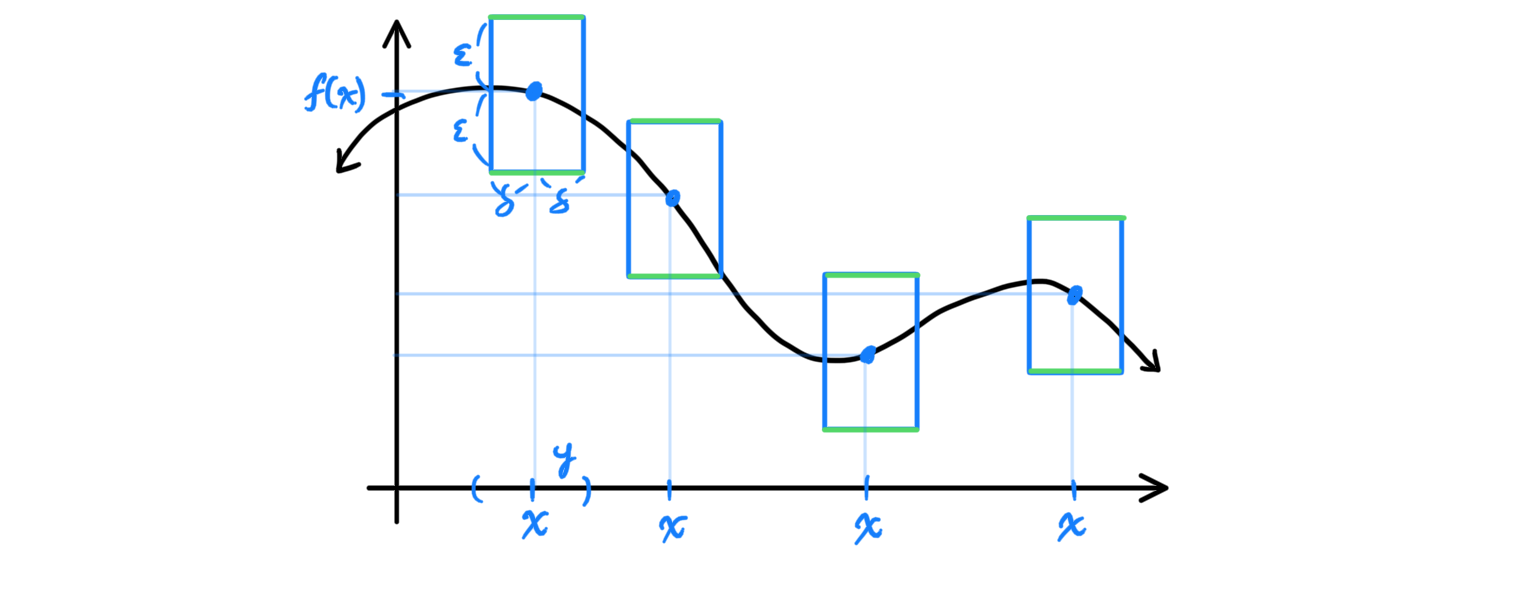
\includegraphics[scale=0.3]{img/Double_Epsilon_Delta_Uniform_Continuity.PNG}
  \end{center}
  Uniform continuity means that the box above does not change dimensions no matter where the point is (hence, the name uniform). Therefore, given a certain $\epsilon > 0$, the way we choose $\delta$ is only dependent on $\epsilon$, and so it must be a function of $\epsilon$: 
  \[\delta = \delta(\epsilon)\]
  However, in continuity, there just has to exist \textbf{some} $\delta$-neighborhood of $x$ such that its image is contained in the $\epsilon$-neighborhood of $f(x)$. There are no restrictions on the dimensions of this box; it just has to exist. 
  \begin{center}
      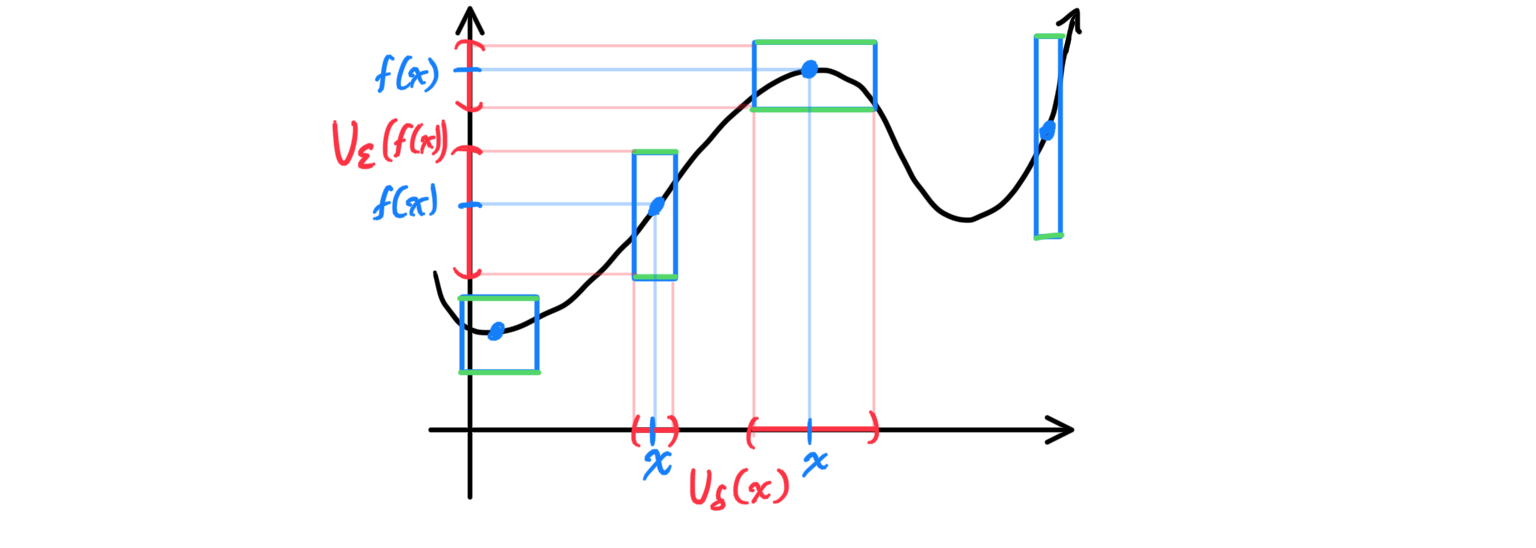
\includegraphics[scale=0.28]{img/Regular_Continuity_Box_Visual.PNG}
  \end{center}

  \begin{lemma}
    If $f$ is uniformly continuous on the set $E$, it is continuous at each point of that set. However, the converse is not generally true. 
  \end{lemma}

  \begin{theorem}[Cantor's Theorem on Uniform Continuity]
  A function that is continuous on a closed interval is uniformly continuous on that interval. 
  \end{theorem}


  \begin{example}
    Let $f: \mathbb{R} \longrightarrow \mathbb{R}, \; f(x) = 3x+7$. Then $f$ is uniformly continuous. Choose $\epsilon > 0$. Let $\delta = \epsilon / 3$. Choose $x, y \in \mathbb{R}$ and assume $|x-y| < \delta$. Then, 
    \[ | f(x) - f(y) | = | 3x + 7 - 3 y - 7 | = 3 |x-y| < 3 \delta = \epsilon\]
  \end{example}

  \begin{example}
    Let $f: (0, 4) \subset \mathbb{R} \longrightarrow \mathbb{R}, \; f(x) = x^2$. Then $f$ is uniformly continuous on $(0, 4)$. Choose $\epsilon > 0$. Let $\delta = \epsilon / 8$. Choose $x, y \in (0, 4)$ and assume $|x-y| < \delta$. Then, 
    \[ |f(x) - f(y)| = |x^2 - y^2| = (x+y) |x-y| < (4+4) |x-y| = 8\delta = \epsilon\]
  \end{example}

  In both examples, the function satisfied an inequality of form 
  \[ |f(x_1) - f(x_2)| \leq M |x_1 - x_2|\]
  this is called the Lipshitz inequality. 

\subsection{Lipshitz Continuity}

  Lipshitz continuity is a strong form of uniform continuity for functions. Intuitively, a Lipshitz continuous function is limited in how fast it can change (by the Lipshitz constant). 

  \begin{definition}[Lipshitz Continuous Function]
    Given $f: E \subset \mathbb{R} \longrightarrow \mathbb{R}$, $f$ is \textbf{Lipshitz continuous} if there exists a positive real constant $M$ such that for all real $x, y \in E$, 
    \[\big| f(x) - f(y) \big| \leq M \big| x - y \big|\]
    The corresponding $M$ is called the \textbf{Lipshitz constant}, and the smallest constant $M$ satisfying this inequality is called the \textbf{best Lipshitz constant}. 

    Note that Lipshitz continuity pops up as a very natural extension of uniform continuity. The inequality above just means that given an $\epsilon$, we can choose a $\delta$ such that a linear multiple of $\delta$ is always greater than $\epsilon$. This means that Lipshitz continuity is just uniform continuity such that the $\delta$ function is linear:  
    \[\delta = \delta(\epsilon) = \frac{1}{M} \epsilon\]
    \begin{center}
        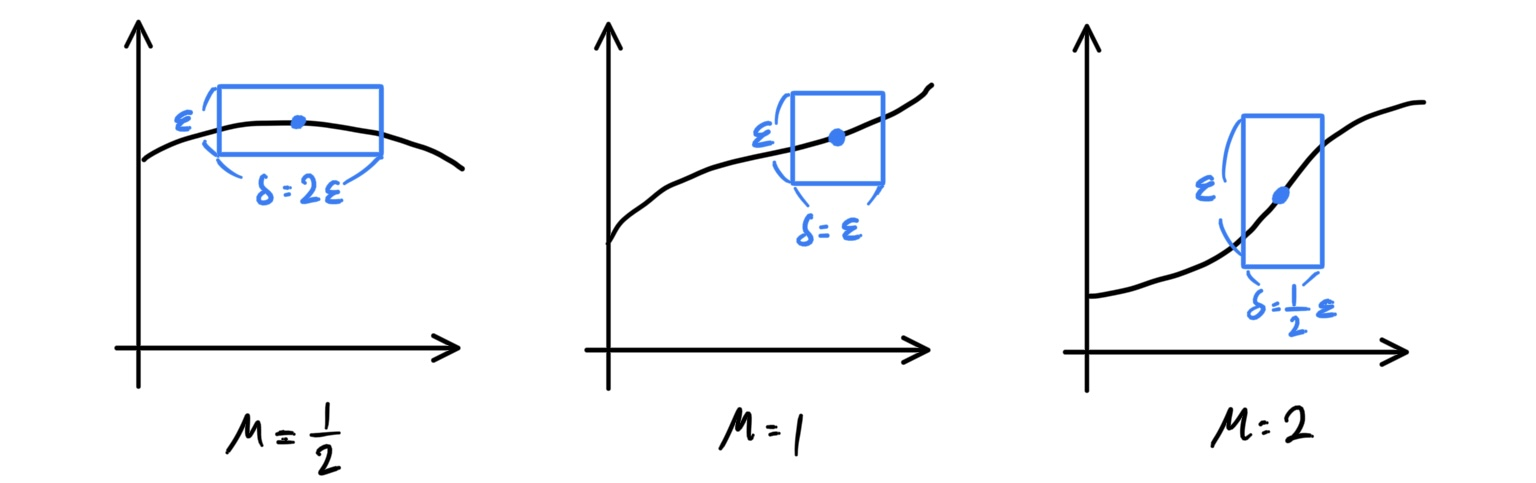
\includegraphics[scale=0.25]{img/Lipshitz_Continuity.jpg}
    \end{center}
  \end{definition}

  Another way to interpret uniform continuity is by seeing that the derivative of $f$ is bounded by the slope $M$. 
  \begin{center}
      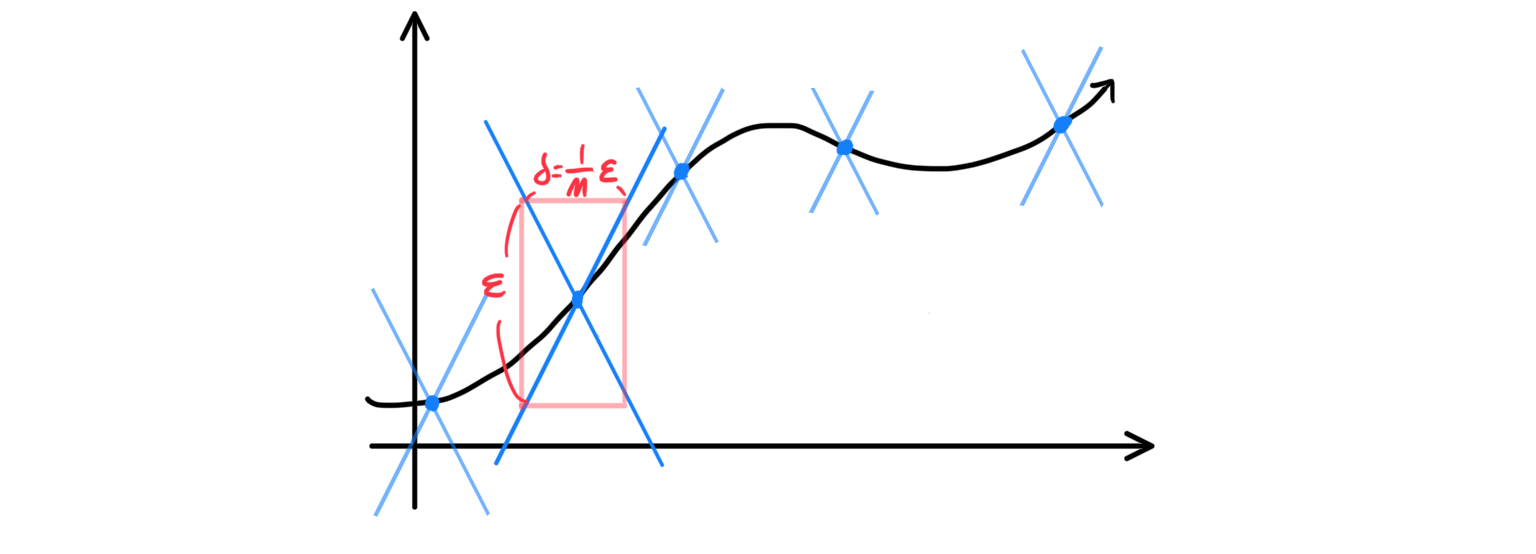
\includegraphics[scale=0.3]{img/Lipshitz_Continuity_Slope_Bound.PNG}
  \end{center}
  This slope bound implies that for every pair of points on the graph of this function, the absolute value of the slope of the line connecting them is not greater than $M'$. The smallest $M'$ is the best Lipshitz constant. 

  \begin{definition}[Bi-Lipshitz Continuity]
    A function $f: E \subset \mathbb{R}$ is \textbf{Bi-Lipshitz continuous} if there exists constant $M\geq 1$ such that for all real $x, y \in E$, 
    \[ \frac{1}{M} |x - y| \leq |f(x) - f(y)| \leq M |x - y|\]
    A visual of this map is shown, where the function $f$ must always land in the shaded green area. 
    \begin{center}
        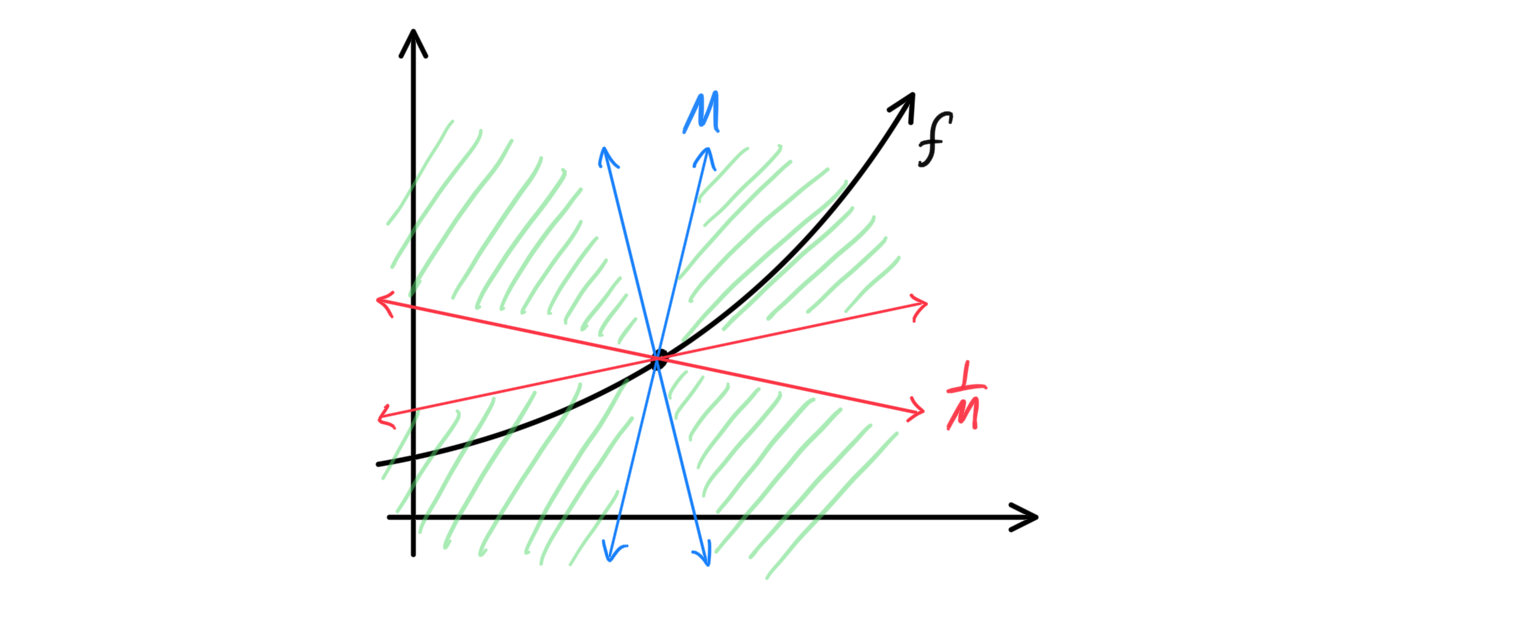
\includegraphics[scale=0.25]{img/BiLipshitz_Map.PNG}
    \end{center}
    It immediately follows that for $x \neq y$, $ |f(x) - f(y)|$ cannot equal $0$, which means that a bilipshitz map is injective. A bilipshitz map is really just Lipshitz map with its inverse also being Lipshitz. 
  \end{definition}

  \begin{proposition}
  A bilipshitz map $f$ is a homeomorphism onto its image. 
  \end{proposition}

\subsection{Discontinuity}

  \begin{definition}[Discontinuity]
    If the function $f: E \longrightarrow \mathbb{R}$ is not continuous at a point of $E$, then this point is called a \textbf{point of discontinuity}, or simply a \textbf{discontinuity} of $f$. 

    That is, $a$ is a point of discontinuity of $f$ if for some neighborhood $V(f(a))$ of $f(a)$, there exists no neighborhood of $a$ whose image under the mapping $f$ is contained in $V(f(a))$. 
    There are three types of discontinuities: 
    \begin{enumerate}
      \item A \textbf{removable discontinuity} is characterized by the fact that the limit $\lim_{x \rightarrow a} f(x) = A$ exists, but $A \neq f(a)$. \begin{center}
          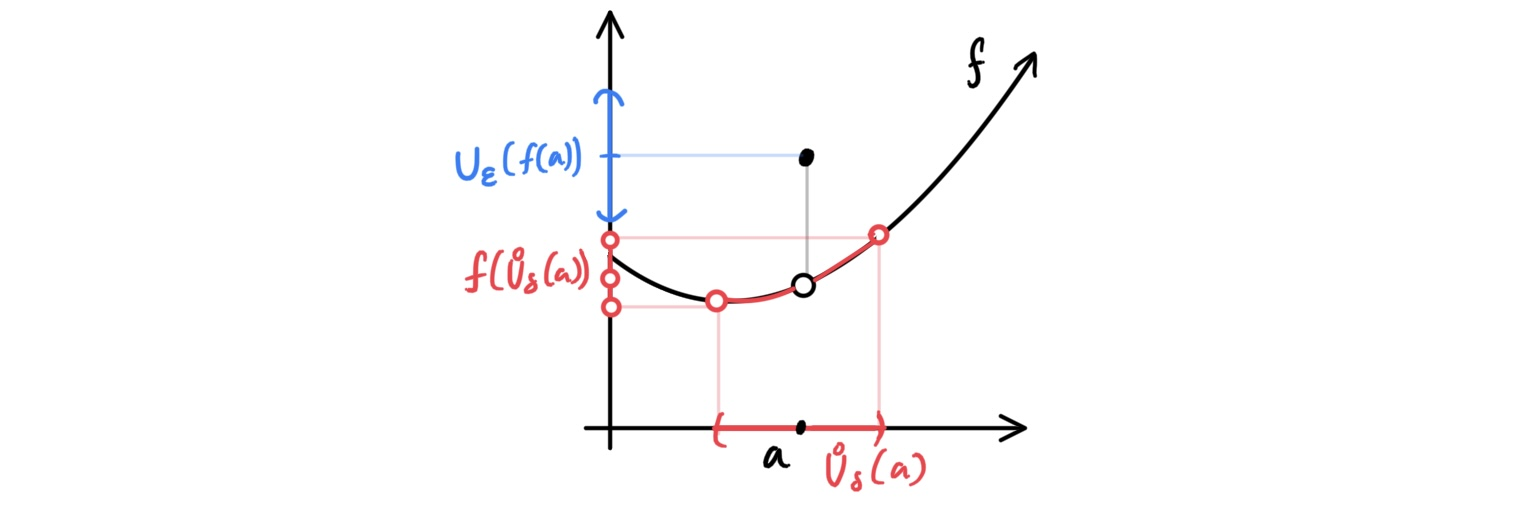
\includegraphics[scale=0.23]{img/Removable_Discontinuity.PNG}
      \end{center}
      This means that we can modify $f$ and define a new function $\Tilde{f}: E \longrightarrow \mathbb{R}$ as
      \[\Tilde{f}(x) = \begin{cases}
      f(x), & x \in E \setminus a \\
      A, & x = a
      \end{cases}\]
      which would be continuous on $E$. 
      \item A \textbf{discontinuity of first kind}, also known as a jump/step discontinuity, is characterized by both the left and right-hand limits 
      \[\lim_{x \rightarrow a-0} f(x) \text{ and } \lim_{x \rightarrow a+0} f(x)\]
      existing, but at least one of them is not equal to the value $f(a)$ that the function assumes at $a$. 
      \begin{center}
          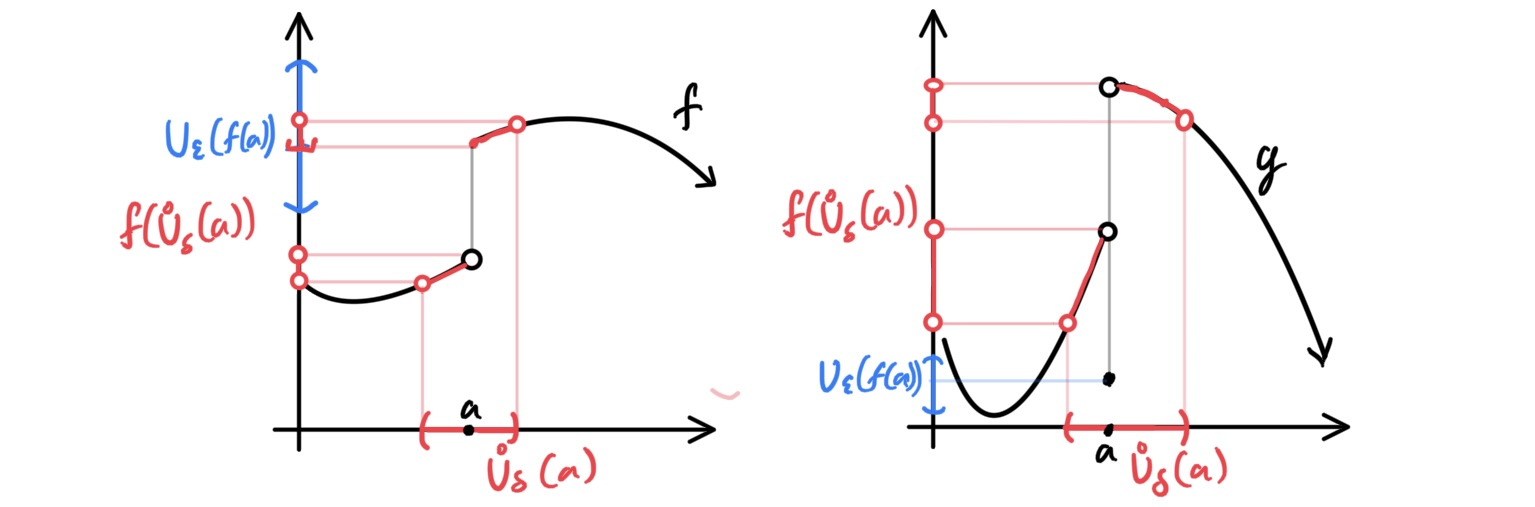
\includegraphics[scale=0.23]{img/Discontinuity_First.PNG}
      \end{center}
      \item A \textbf{discontinuity of second kind}, also known as an essential discontinuity, is characterized by at least one of the two limits 
      \[\lim_{x \rightarrow a-0} f(x) \text{ and } \lim_{x \rightarrow a+0} f(x)\]
      not existing. 
      \begin{center}
          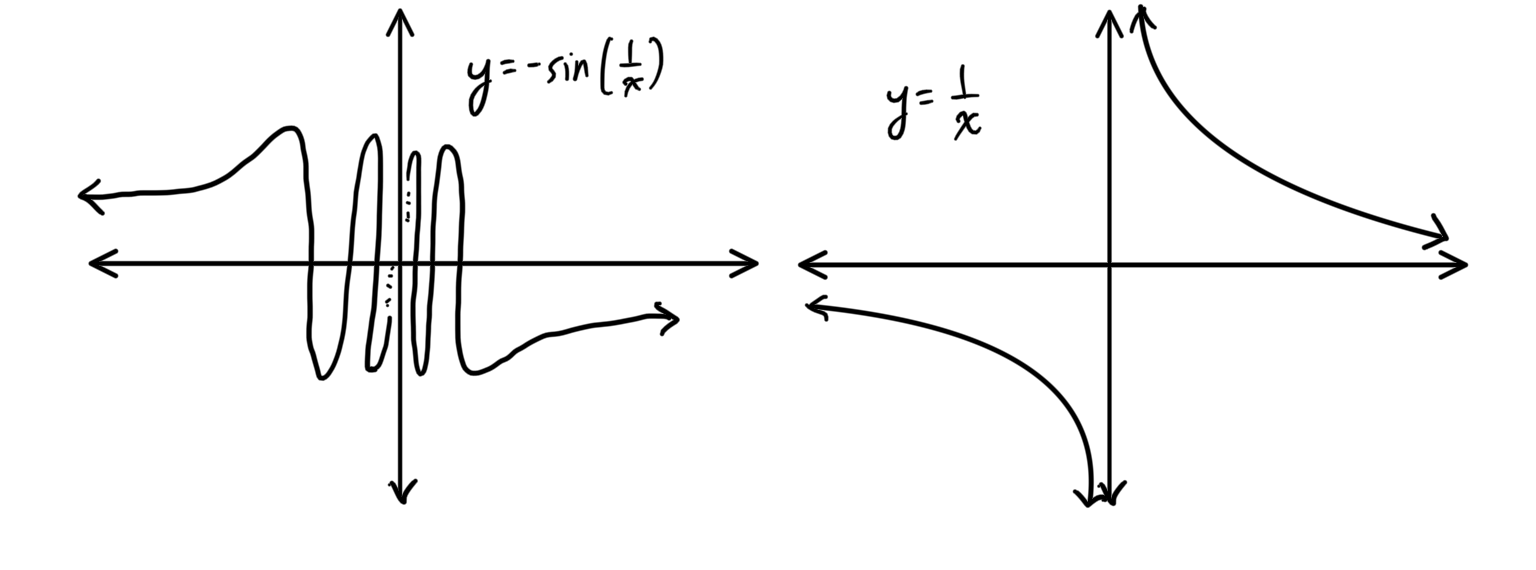
\includegraphics[scale=0.23]{img/Discontinuity_Second.PNG}
      \end{center}
    \end{enumerate}
    Note that strictly speaking, a removable discontinuity is really a discontinuity of first kind, but in this context we distinguish them. 
  \end{definition}

  \begin{example}[Dirichlet Function]
    The Dirichlet function, defined
    \[\mathcal{D}(x) = \begin{cases}
    1, & \text{ if } x \in \mathbb{Q} \\
    0, & \text{ if } x \in \mathbb{R} \setminus \mathbb{Q} 
    \end{cases}\]
    is discontinuous at every point, and obviously all of its discontinuities are of second kind, since in every interval there are both rational and irrational numbers and therefore there exists no limit at any point $a \in \mathbb{R}$. 

    More specifically, given any point $a \in \mathbb{R}$, assume that $a$ is rational. We can set $\epsilon = 0.1$-neighborhood around the value $1$, but no matter how small we let $\delta$, the interval $(a - \delta, a + \delta)$ will contain both rationals and irrationals, meaning that it will map to $\{0,1\}$ always, which is not fully contained in $(0.9, 1.1)$.  
  \end{example}

  Here is a slightly more interesting example. 

  \begin{example}[Riemann Function]
    Let the Riemann function $\mathcal{R}$ be defined
    \[\mathcal{R}(x) = \begin{cases}
    \frac{1}{n}, & \text{ if } x = \frac{m}{n} \in \mathbb{Q}, \text{ where gcd}(m, n) = 1 \\
    0, & \text{ if } x \in \mathbb{R} \setminus \mathbb{Q}
    \end{cases}\]
    We first note that for any point $a \in \mathbb{R}$, any bounded neighborhood $U(a)$ of it, and any number $N \in \mathbb{N}$, the neighborhood $U(a)$ contains only a finite number of rational numbers $\mathbb{m}{n}$, where $n < N$. By shrinking the neighborhood, we can assume that the denominators of all rational numbers in the neighborhood are larger than $N$. We can visualize why this is by seeing that rational numbers with larger denominators have smaller "gaps" between them. 
    \begin{center}
        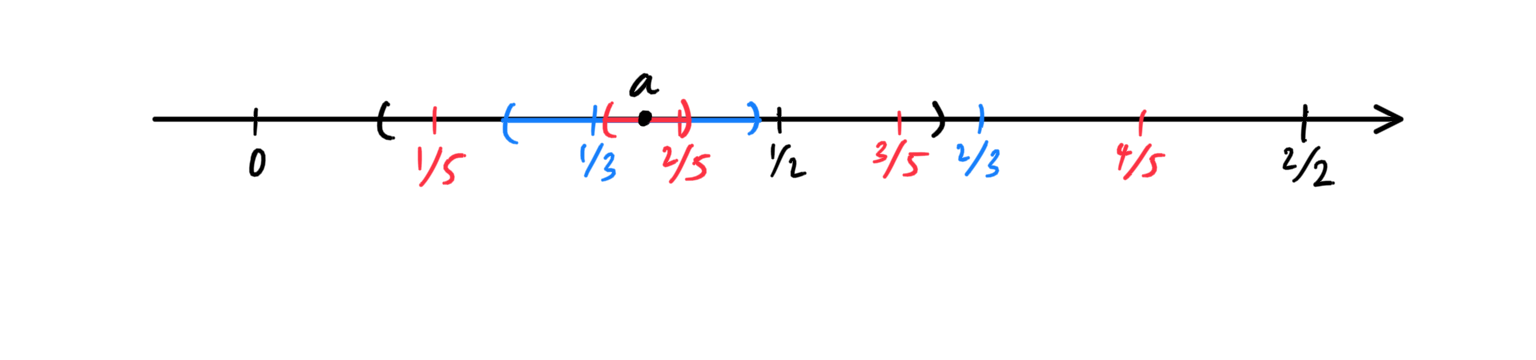
\includegraphics[scale=0.23]{img/Rationals_Spread_Apart.PNG}
    \end{center}
    Thus, at any point $x \in U(a) \setminus a$, we have 
    \[\big| \mathcal{R}(x) \big| < \frac{1}{N}\]
    and therefore
    \[\lim_{x \rightarrow a} \mathcal{R} (x) = 0\]
    at any point $a \in \mathbb{R} \setminus \mathbb{Q}$. Hence, the Riemann function is continuous at any irrational number. 
  \end{example}


 
\section{Differentiation}
 
\section{Integration}

  \subsection{Construction of the Riemann Integral}

    We shall first define the integral using the familiar notation of Riemann sums. 

    \begin{definition}[Partitions with Distinguished Points]
      A \textbf{partition} $P$ of a closed interval $[a, b]$, $a < b$, is a finite system of points $x_0, \ldots, x_n$ of the interval such that
      \[a = x_0 < x_1 < x_2 < \ldots < x_n = b\]
      The intervals $[x_{i-1}, x_i]$, $i = 1, 2, \ldots, n$, are called the \textbf{intervals} of the partition $P$. The largest of the lengths of the intervals of the partition $P$, denoted $\lambda(P)$, is called the \textbf{mesh} of the partition. 

      A \textbf{partition with distinguished points} $(P, \xi)$ on the closed interval $[a, b]$ is a partition $P$ of $[a,b]$ along with the set of $n$ points 
      \[\xi_1 \in [x_0, x_1], \xi_2 \in [x_1, x_2], \ldots, \xi_n \in [x_{n-1}, x_n]\]
      The $n$-tuple of $\xi_i$'s is denoted by the single letter $\xi$
      \[\xi = (\xi_1, \xi_2, \ldots, \xi_n)\]
    \end{definition}

    This naturally leads to the following construction. 

    \begin{definition}[Riemann Sums]
      If a function $f$ is defined on a closed interval $[a, b]$ and $(P, \xi)$ is a partition with distinguished points on this closed interval, the sum
      \[\sigma(f; P, \xi) \equiv \sum_{i=1}^n f(\xi_i)\, \Delta x_i, \text{ where } \Delta x_i = x_i - x_{i-1},\]
      is the \textbf{Riemann sum} of the function $f$ corresponding to the partition $(P, \xi)$ with distinguished points on $[a, b]$. 
      \begin{center}
          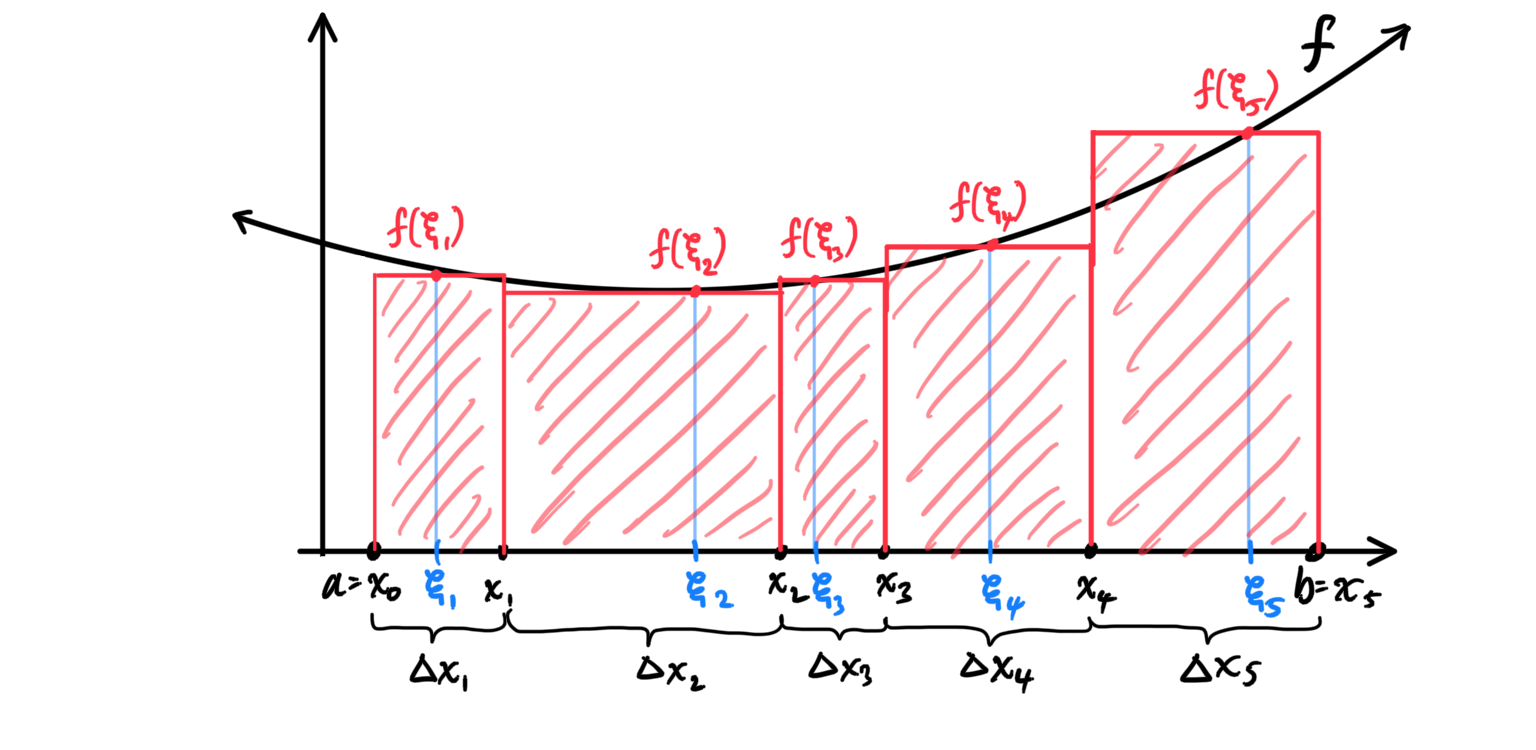
\includegraphics[scale=0.25]{img/Riemann_Sum_with_Partitions_Points.PNG}
      \end{center}
      Thus, when a function $f$ is fixed, the Riemann sum $\sigma (f; P, \xi)$ is a mapping that takes in a partition with distinguished points $p = (P, \xi)$ on the closed interval $[a, b]$ and outputs a number representing the total area of the Riemann sums. That is, for a fixed $f$ and some input $p = (P, \xi)$, we can define the function 
      \[\Phi: \mathcal{P} \longrightarrow \mathbb{R}, \;\;\; \Phi(p) \equiv \sigma(f; p) \equiv \sigma(f; (P, \xi))\]
      that takes in a partition with distinguished points on $[a,b]$ and outputs the corresponding Riemann sum for that fixed $f$. 
    \end{definition}

    \begin{definition}[Riemann Integral]
      The number $\int_a^b f(x)\,dx$ is the \textbf{Riemann integral} of the function $f$ on the closed interval $[a, b]$ if for every $\epsilon>0$ there exists a $\delta>0$ such that
      \[\Bigg| \int_a^b f(x)\,dx - \sum_{i=1}^n f(\xi_i) \Delta x_i \Bigg| < \epsilon\]
      for any partition $(P, \xi)$ with distinguished points on $[a, b]$ whose mesh $\lambda(P)$ is less than $\delta$. We can view this as a limit where $n \rightarrow \infty$, but there is a problem since we can increase the partition within different subsets of $[a,b]$, leading to multiple values of convergence. 
      \begin{center}
          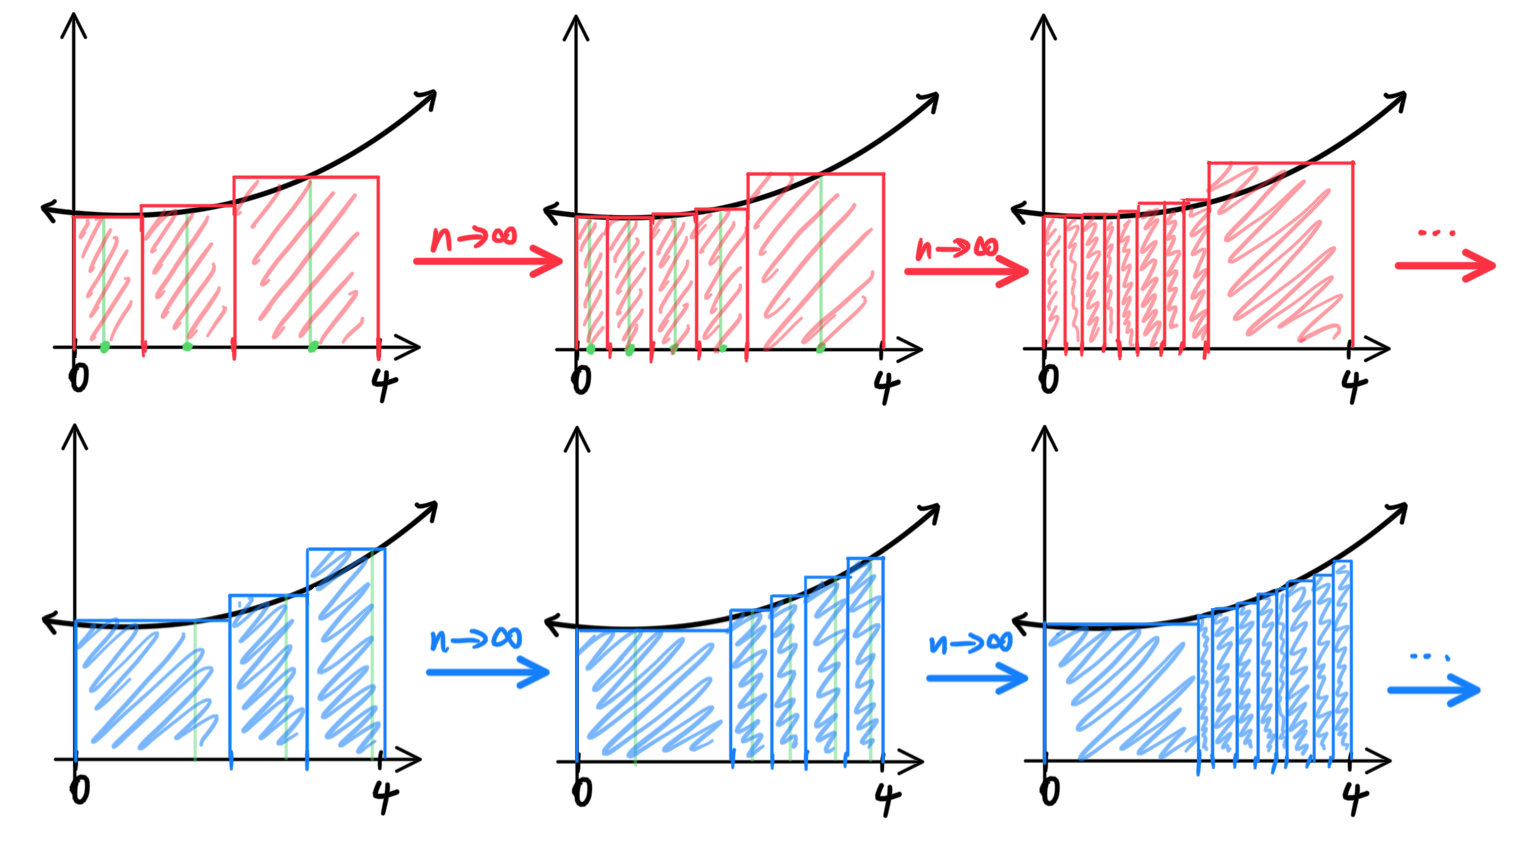
\includegraphics[scale=0.28]{img/Riemann_Integral_Converging_onto_2_Numbers.PNG}
      \end{center}
      Rather, we can set the mesh $\lambda(P)$ to approach $0$, which would take care of the problems. We can visualize this by imagining the lengths of the rectangles converging "uniformly."
      \begin{center}
          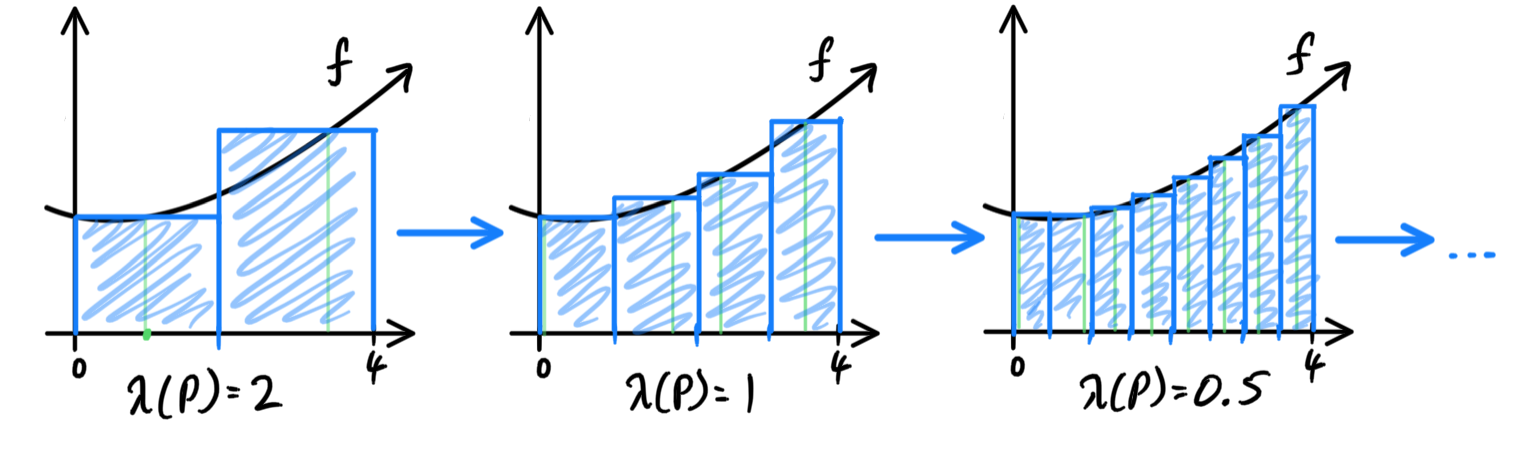
\includegraphics[scale=0.28]{img/Riemann_Integral_Limit_Mesh_goes_to_0.PNG}
      \end{center}
      Therefore, we can culminate by defining the Riemann integral of $f(x)$ over $[a,b]$ as 
      \[\int_a^b f(x)\,dx \equiv \lim_{\lambda(P) \rightarrow 0} \sum_{i=1}^n f(\xi_i) \lambda x_i\]
    \end{definition}

  \subsubsection{Conditions for Integrability}

    \begin{definition}[Riemann Integrable Functions]
      A function $f$ is \textbf{Riemann integrable} on the closed interval $[a, b]$ if 
      \[\int_a^b f(x)\,dx \equiv \lim_{\lambda(P) \rightarrow 0} \sum_{i=1}^n f(\xi_i) \lambda x_i\]
      is defined, i.e. if the limit of the right-hand side of Riemann sums exists as $\lambda(P) \rightarrow 0$ (that is, the Riemann integral of $f$ is defined). 

      Furthermore, the set of Riemann-integrable functions on a closed interval $[a, b]$ is denoted $\mathcal{R}[a,b]$. 
    \end{definition}

    Remember that the Riemann integral, as complicated as the formula is, is still a limit of a function. That means that we can apply the Cauchy criterion to it to determine convergence. 

    \begin{lemma}[Cauchy Criterion on Existence of Riemann Integral]
      Given a function $f$, the integral of $f$ over $[a, b]$, defined
      \[\int_a^b f(x)\,dx \equiv \lim_{\lambda(P) \rightarrow 0} \sum_{i=1}^n f(\xi_i) \lambda x_i\]
      exists if and only if for every $\epsilon>0$, there exists a $\delta>0$ such that 
      \[\big| \sigma(f; P^\prime, \xi^\prime) - \sigma(f; P^{\prime\prime}, \xi^{\prime\prime} \big| < \epsilon\]
      or, what is the same, 
      \[\Bigg| \sum_{i=1}^{n^\prime} f(\xi_i^\prime) \Delta x_i^\prime - \sum_{i=1}^{n^{\prime\prime}} f^(\xi_i^{\prime\prime}) \Delta x_i^{\prime\prime} \Bigg| < \epsilon\]
      for any partitions $(P^\prime, \xi^\prime)$ and $(P^{\prime\prime}, \xi^{\prime\prime})$ with distinguished points on the interval $[a, b]$ with
      \[\lambda(P^\prime), \lambda(P^{\prime\prime}) < \delta\]
      In words, this means that for any $\epsilon>0$ that we choose, there always exists a $\delta>0$ such that \textbf{any} two Riemann sums with mesh size \textbf{both} smaller than $\delta$ will have an error difference of less than $\epsilon$. \begin{center}
          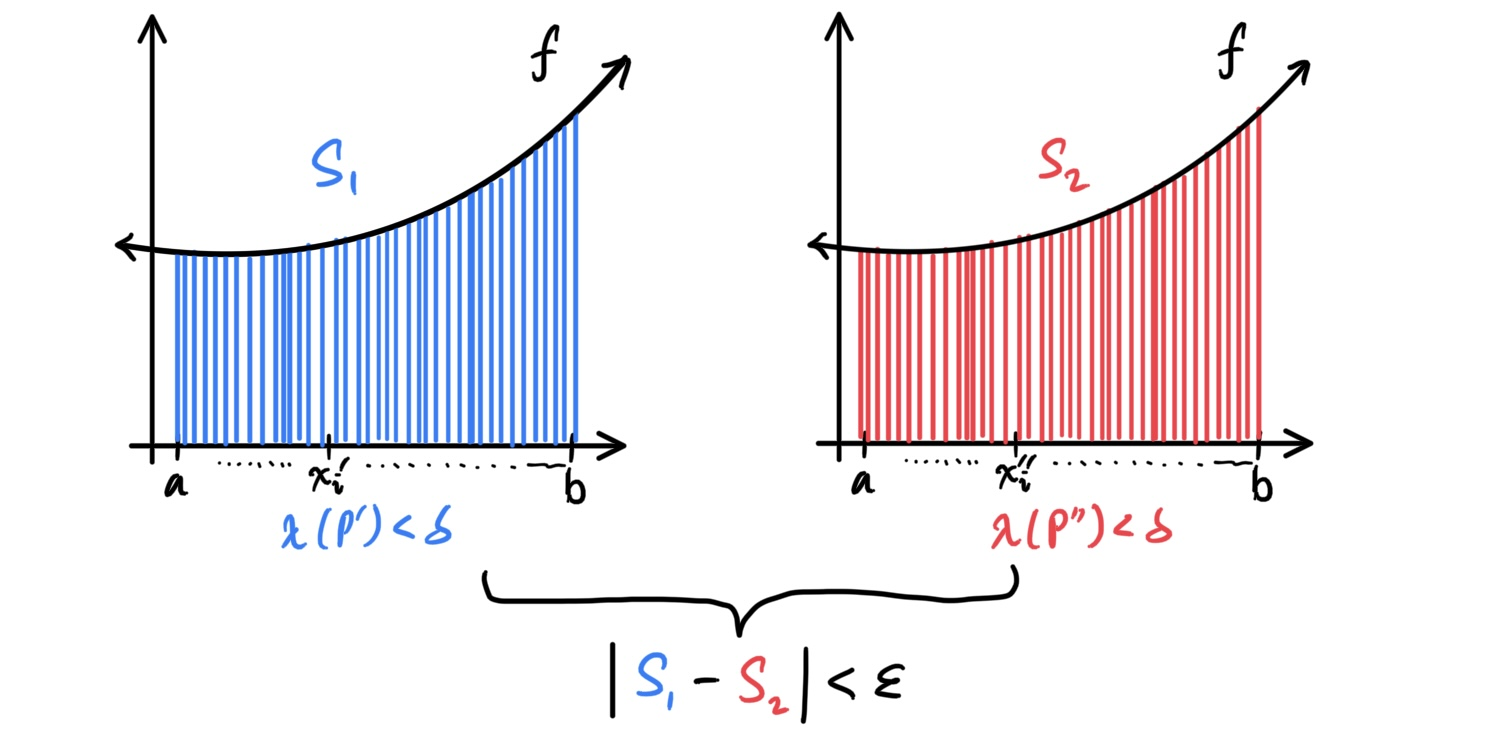
\includegraphics[scale=0.25]{img/Cauchy_Criterion_of_Riemann_Integral.jpg}
      \end{center}
    \end{lemma}

    \begin{theorem}[Necessary Condition for Integrability]
    A necessary condition for $f$ defined on a closed interval $[a, b]$ to be Riemann integrable on $[a, b]$ is that $f$ be bounded on $[a, b]$. That is, 
    \[f \in \mathcal{R}[a, b] \implies f \text{ is bounded on } [a, b]\]
    We can clearly see the necessity of $f$ being bounded by looking at the contrapositive of the following statement. 
    \end{theorem}

    \begin{theorem}[Refinement]
    Given a partition $P$ on interval $[a, b]$, recall that we have points $x_0, \ldots, x_n$ such that
    \[a = x_0 < x_1 < \ldots < x_n = b\]
    Here we introduce new notation: 
    \begin{enumerate}
      \item $\Delta_i$ denotes the interval $[x_{i-1}, x_i]$
      \item $\Delta x_i$ denotes the difference $x_i - x_{i-1}$, i.e. the length of $\Delta_i$
    \end{enumerate}
    If a partition $\Tilde{P}$ of the closed interval $[a, b]$ is obtained from the partition $P$ by the addition of new points to $P$, we call $\Tilde{P}$ a \textbf{refinement} of $P$. 

    When a refinement $\Tilde{P}$ of a partition $P$ is constructed, some (perhaps all) of the closed intervals $\Delta_i = [x_{i-1}, x_i]$ of the partition $P$ themselves undergo partitioning. 
    \[x_{i-1} = x_{i0} < x_{i1} < \ldots < x_{in_i} = x_i\]
    In that connection, it will be useful to label to points of $\Tilde{P}$ by double indices, where in the notation $x_{ij}$ the first index $i$ means that 
    \[x_{ij} \in \Delta_i = [x_{i-1}, x_i]\]
    and the second index $j$ is the ordinal number of the point on the closed interval $\Delta_i = [x_{i-1}, x_i]$. Therefore, it is natural to set the notations
    \begin{enumerate}
      \item $\Delta_{ij} = [x_{i j-1}, x_{ij}]$
      \item $\Delta x_{ij} = x_{ij} - x_{ij-1}$
    \end{enumerate}
    This means that 
    \[\Delta x_i = \Delta x_{i1} + \Delta x_{i2} + \ldots + \Delta x_{in_i}\]
    which can be visualized below
    \begin{center}
      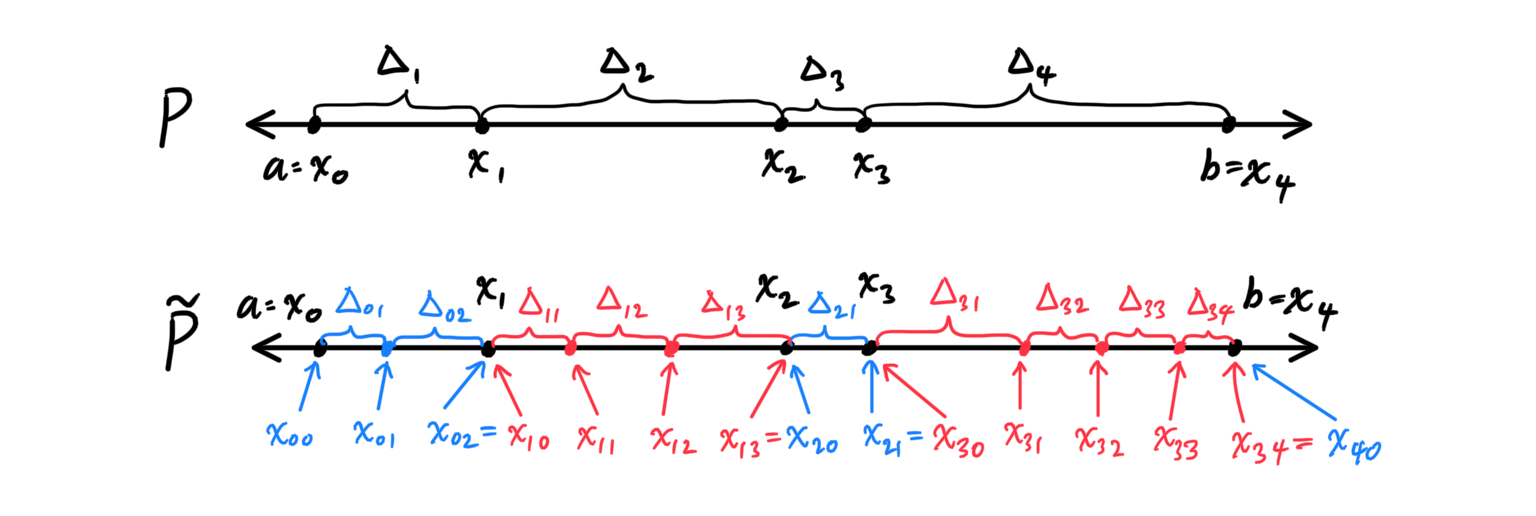
\includegraphics[scale=0.25]{img/Refinement_Definition_Analysis.PNG}
    \end{center}
    \end{theorem}

    \begin{example}[Union of Partitions as a Refinement]
    For some interval $[a, b]$, given partitions $P^\prime$ ($a = x_0 < \ldots < x_n = b$) and $P^{\prime\prime}$ ($a = y_0 < \ldots < y_n = b$), the union of the two partitions $\Tilde{P} = P^\prime \cup P^{\prime\prime}$ is a refinement of both $P^\prime$ and $P^{\prime\prime}$. 
    \begin{center}
        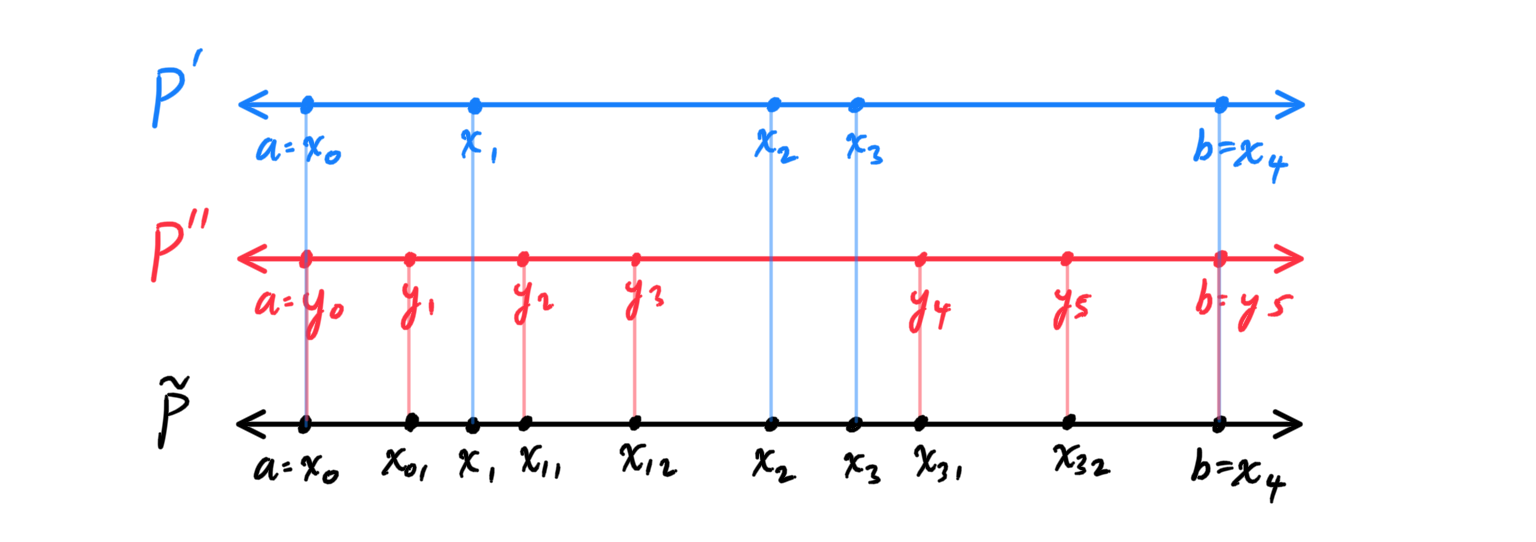
\includegraphics[scale=0.25]{img/Refinement_as_Union_of_Partitions.PNG}
    \end{center}
    \end{example}
    
    Recall that $\omega(f; E)$ denotes the oscillation of the function $f$ on the set $E$; that is, 
    \[\omega(f; E) \equiv \sup_{x^\prime, x^{\prime\prime} \in E} \big| f(x^\prime) - f(x^{\prime\prime})\big|\]
    In particular, $\omega(f; \Delta_i)$ is the oscillation of $f$ on the closed interval $\Delta_i$. 

    \begin{theorem}[Sufficient Condition for Integrability]
    Let $f$ be a bounded on a closed interval $[a, b]$ such that for every $\epsilon > 0$ there exists a number $\delta>0$ such that
    \[\sum_{i=1}^n \omega(f; \Delta_i) \Delta x_i < \epsilon\]
    for any partition $P$ of $[a, b]$ with mesh $\lambda(P) < \delta$. This is equivalent to saying that
    \[\lim_{\lambda(P) \rightarrow 0} \sum_{i = 1}^n \omega (f; \Delta_i) \, \Delta x_i = 0\]
    Then, $f$ is integrable. We can visualize
    \[\sum_{i=1}^n \omega(f; \Delta_i) \Delta x_i\]
    as the following sum of rectangles below. 
    \begin{center}
        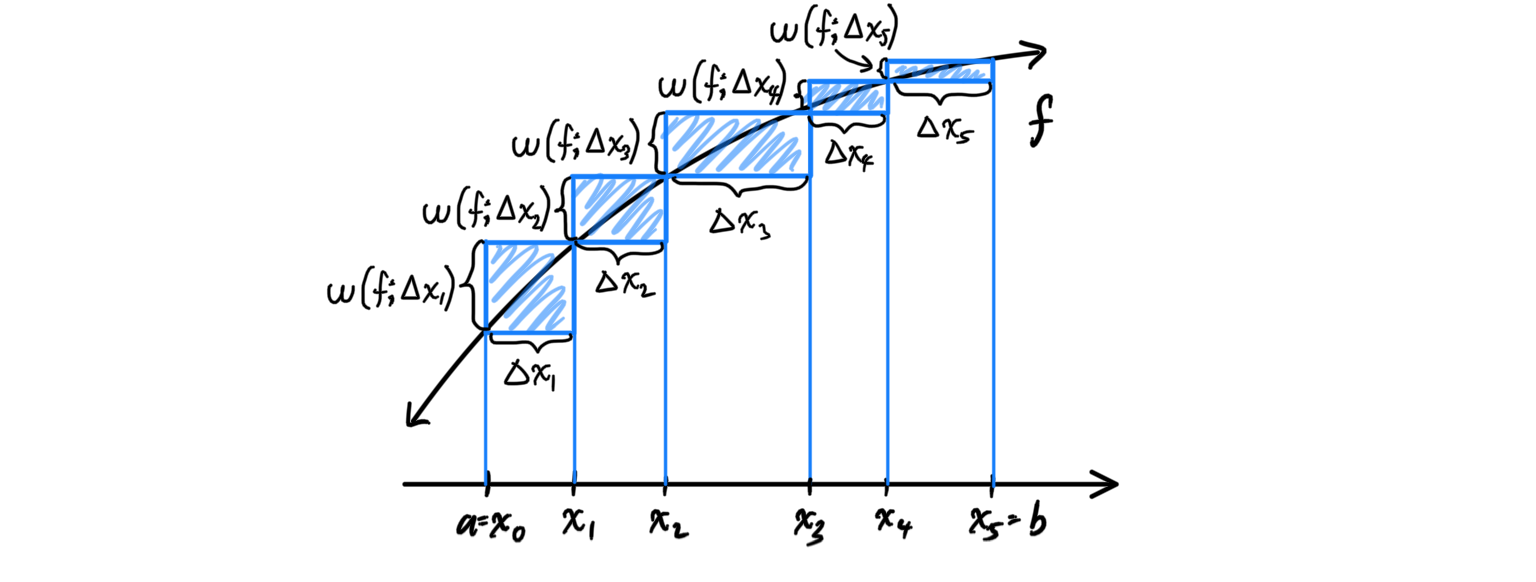
\includegraphics[scale=0.25]{img/Sufficient_Condition_for_Integrability.PNG}
    \end{center}
    What the theorem states, visually, is that as we make all the rectangles smaller and smaller (by putting a limit on the mesh $\lambda(P)<\delta$), we can make the sum of all these rectangles also arbitrarily small. 
    \end{theorem}

    \begin{corollary}[Integrability of Continuous Functions]
    Every continuous function on a closed interval is integrable on that closed interval. That is, 
    \[f \in C[a, b] \implies f \in \mathcal{R}[a, b]\]
    \end{corollary}

    We can actually make a stronger claim. 

    \begin{corollary}[Integrability of Discontinuous Functions]
    If a bounded function $f$ on a closed interval $[a, b]$ is continuous everywhere except at a finite set of points, then $f \in \mathcal{R}[a, b]$. 
    \end{corollary}

    \begin{corollary}[Integrability of Monotonic Functions]
    A bounded monotonic function on a closed interval is integrable on that interval. 
    \begin{center}
        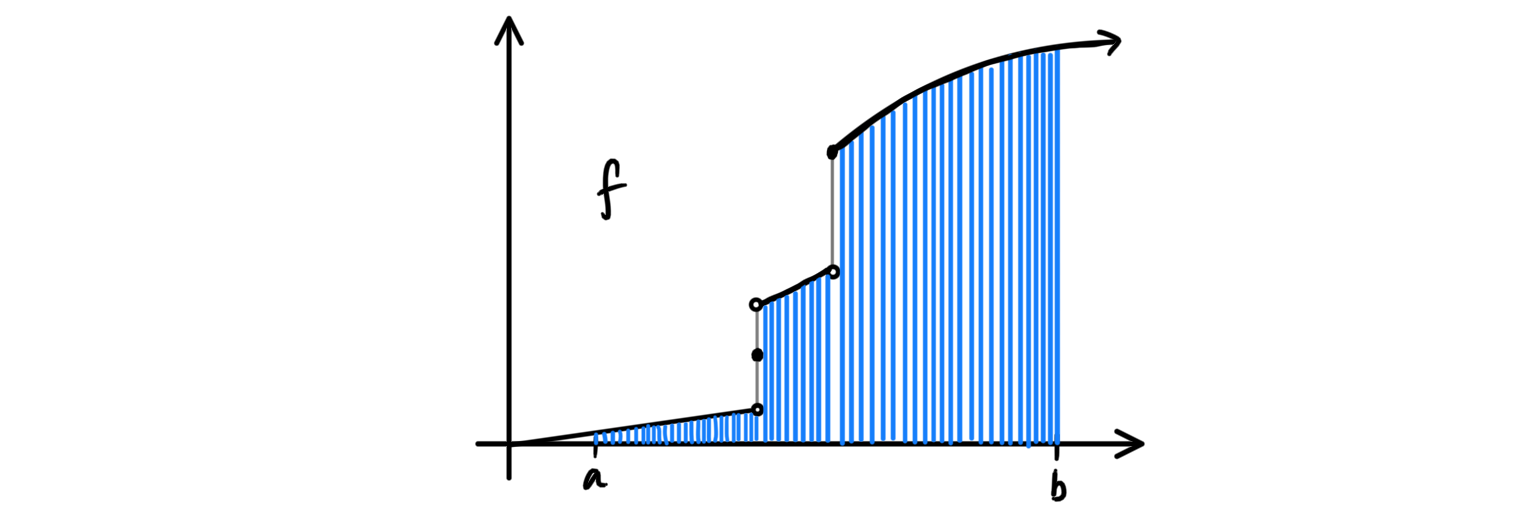
\includegraphics[scale=0.25]{img/Integrability_of_Monotonic_Function.PNG}
    \end{center}
    \end{corollary}

    \begin{definition}[Upper, Lower Riemann Sums]
      Let $f: [a, b] \longrightarrow \mathbb{R}$ be a real-valued function that is defined and bounded on the closed interval $[a, b]$, and let $P$ be a partition of $[a, b]$, and let $\Delta_i$ ($i = 1, 2, \ldots, n$) be the intervals of the partition $P$. Let 
      \begin{align*}
          m_i &= \inf_{x \in \Delta_i} f(x) \\
          M_i &= \sup_{x \in \Delta_i} f(x)
      \end{align*}
      be the infimum and supremum of $f$ over $\Delta x_i$. Then, the sums
      \begin{align*}
          s(f; P) & \equiv \sum_{i = 1}^n m_i \, \Delta x_i \\
          S(f; P) & \equiv \sum_{i=1}^n M_i \, \Delta x_i
      \end{align*}
      are respectively called the \textbf{lower} and \textbf{upper Riemann sums} of the function $f$ on the interval $[a, b]$ corresponding to the partition $P$ of that interval. 

      Given an arbitrary partition $(P, \xi)$ with distinguished points on $[a, b]$, it is clear that
      \[s(f; P) = \inf_{\xi} \sigma(f; P, \xi) \leq \sigma(f; P, \xi) \leq \sup_{\xi} \sigma(f; P, \xi) = S(f; P)\]
    \end{definition}

    \begin{theorem}
    A bounded real-valued function $f: [a, b] \longrightarrow \mathbb{R}$ is Riemann integrable on $[a, b]$ if and only if the following limits exist and are equal to each other. 
    \[\underline{I} \equiv \lim_{\lambda(P) \rightarrow 0} s(f; P) = \lim_{\lambda(P) \rightarrow 0} S(f; P) \equiv \overline{I}\]
    When the relation is true, then the integral is this common value. 
    \[\int_a^b f(x) \,dx = \underline{I} = \overline{I}\]
    \end{theorem}

    Note that this condition of the upper and lower Riemann sums converging to the same value and the condition that 
    \[\lim_{\lambda(P) \rightarrow 0} \sum_{i = 1}^n \omega (f; \Delta_i) \, \Delta x_i = 0\]
    are the same. For we can see that the rectangles visualized from the equation above are the exact same rectangles formed by $S(f; P) - s(f; P)$! 
    \begin{center}
        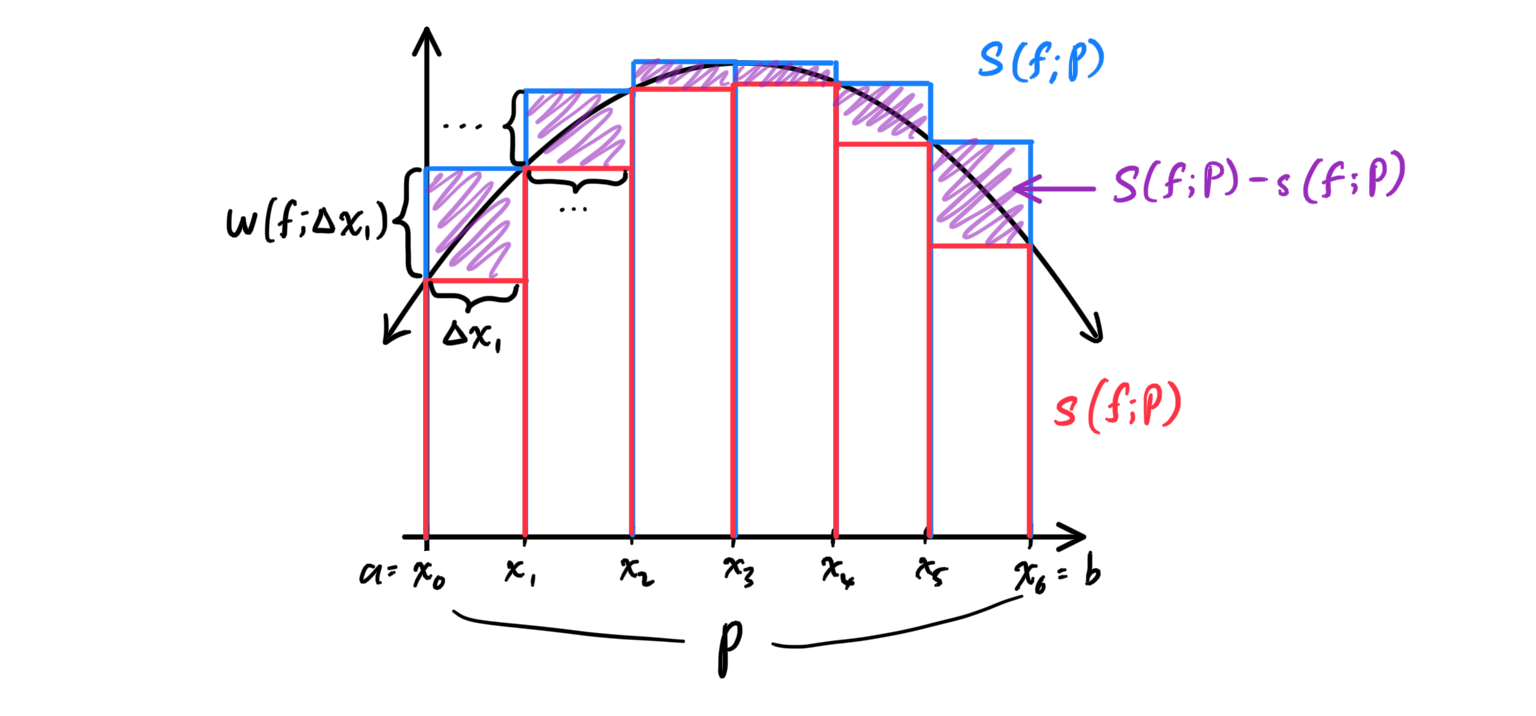
\includegraphics[scale=0.3]{img/Equivalent_Conditions_for_Integrability.PNG}
    \end{center}

    \subsubsection{The Vector Space of Riemann Integrable Functions}

    \begin{theorem}[The Vector Space of Integrable Functions]
    The set of Riemann integrable functions $\mathcal{R}[a, b]$ over closed interval $[a, b]$ is a vector space. That is, given $f, g \in \mathcal{R}[a, b]$ and $\alpha \in \mathbb{R}$, then
    \begin{enumerate}
      \item $(f + g) \in \mathcal{R}[a, b]$ 
      \item $(\alpha f) \in \mathcal{R}[a, b]$
    \end{enumerate}
    Furthermore, 
    \begin{enumerate}
      \item $|f| \in \mathcal{R}[a, b]$
      \item The restriction of $f$ in any $[c, d] \subset [a, b]$, denoted $f \big|_{[c,d]}$, is in $\mathcal{R}[c,d]$
      \item $(f \cdot g) \in \mathcal{R}[a, b]$
    \end{enumerate}
    \end{theorem}
    \begin{proof}

    \end{proof}

    \subsubsection{Lebesgue's Criterion for Riemann Integrability}
    We give Lebesgue's version of an intrinsic description of a Riemann integrable function. 

    \begin{definition}[Measure]
      A set $E \subset \mathbb{R}$ has \textbf{(Lebesgue) measure zero} if for every number $\epsilon > 0$ there exists a covering of the set $E$ be an at most countable system $\{I_k\}$ of intervals, the sum of whose lengths 
      \[\sum_{k=1}^\infty |I_k| \leq \epsilon\]
      This means that the above series summing up the lengths of the intervals is an absolutely convergent series. 
    \end{definition}

    \begin{lemma}
      We can deduce measures of basic sets. 
      \begin{enumerate}
        \item A finite number of points are sets of measure zero. 
        \item The union of a finite or countable number of sets of measure zero is a set of measure zero. \item A subset of a set of measure zero is itself a set of measure zero. 
        \item A closed interval $[a, b]$ with $a<b$ is not a set of measure zero. 
      \end{enumerate}
    \end{lemma}

    \begin{definition}
      If a property holds at all points of a set $X$ except possible the points of a set of measure zero, we say that this property holds \textbf{almost everywhere on $X$} or \textbf{at almost every point of $X$}. 
    \end{definition}

    Now, we can state Lebesgue's criterion for integrability, which nicely summarizes what we have so far. 

    \begin{theorem}[Lebesgue's Criterion for Integrability]
    A function defined on a closed interval is Riemann integrable on that interval if and only if it is bounded and continuous at almost every point. 
    \end{theorem}

    \begin{example}[Non-Integrability of the Dirichlet Function]
    The Dirichlet function
    \[\mathcal{D}(x) \equiv \begin{cases}
    1, & \text{ for } x \in \mathbb{Q} \\
    0, & \text{ for } x \in \mathbb{R} \setminus \mathbb{Q}
    \end{cases}\]
    on the interval $[0,1]$ is not integrable on that interval. We state two different reasons why. 
    \begin{enumerate}
      \item For any partition $P$ of $[0,1]$ we can find in each interval $\Delta_i$ both a rational point $\xi^\prime_i$ and an irrational point $\xi_i^{\prime\prime}$. Then, we can see that the lower and upper Riemann sums do not necessarily converge to each other since
      \[\sigma(f; P, \xi^\prime) = \sum_{i=1}^n 1 \cdot \Delta x_i = 1 \text{ while } \sigma(f;P, \xi^{\prime\prime}) = \sum_{i=1}^n 0 \cdot \Delta x_i = 0\]
      as $\lambda(P) \rightarrow 0$. 
      \item From the point of view of the Lebesgue criterion the nonintegrability of the Dirichlet function is obvious since $\mathcal{D}(x)$ is discontinuous at every point of $[0, 1]$, which is not a set of measure zero. 
    \end{enumerate}
    \end{example}

    Notice that by the Lebesgue criterion, integrability is a weaker condition than continuity. That is, 
    \[f \text{ continuous } \implies f \text{ Riemann integrable}\]
    but not necessarily the other way around. It turns out that this has consequences when determining the composition of functions. 

    \begin{proposition}[Integrable + Continuous Composition]
    Let $f: I_1 = [a, b] \longrightarrow\mathbb{R}$ be a function that is integrable on $[a, b]$, with Im$\,f = [c, d] = I_2$. Define a continuous (remember, continuity is stronger than integrability) function $g: [c, d] \longrightarrow \mathbb{R}$. Then the composition
    \[g \circ f: [a, b] \longrightarrow \mathbb{R}\]
    is clearly defined and continuous at all the points of $[a, b]$ where $f$ is continuous. But since $f$ is integrable, the union of all the discontinuities in $[a, b]$ must have measure zero, and so it follows that since $[a, b]$ is the same  
    \[g \circ f \in \mathcal{R}[a, b]\]
    Therefore, we can found out that 
    \[f \text{ integrable and } g \text{ continuous} \implies g \circ f \text{ integrable}\]
    as visualized in the commutative diagram below. 
    \[
      \begin{tikzcd}
        I_1 \arrow[r, "f"] \arrow[rr, bend left, "g \circ f"] & I_2 \arrow[r, "g"] & \mathbb{R}
      \end{tikzcd}
    \]
    However, contrary to intuition, 
    \[f \text{ integrable and } g \text{ integrable} \centernot\implies g \circ f \text{ integrable}\]
    \end{proposition}

    We present a counterexample. 
    \begin{example}
    Consider the functions
    \[|sgn|(x) \equiv \begin{cases}
    1 & x \neq 0 \\
    0 & x = 0
    \end{cases}\]
    and the Riemann function 
    \[\mathcal{R}(x) \equiv \begin{cases}
    \frac{1}{n} & x = \frac{m}{n} \in \mathbb{Q}, \gcd(m, n) = 1 \\
    0 & x \in \mathbb{R} \setminus \mathbb{Q}
    \end{cases}\]
    We can see that $\mathcal{R}$ is continuous at all irrational points and discontinuous at all rational points except $0$, meaning that it is integrable ($\mathbb{Q}$ has measure zero). Then, the composition of these two functions is precisely the Dirichlet function
    \[\mathcal{D}(x) = |sgn| \circ \mathcal{R}\]
    which is not integrable. 
    \end{example}

  \subsection{Basic Properties of the Integral}

    One of the most basic properties of the integral is that it is a linear map. 
    \begin{lemma}[Linearity of the Integral]
      Given closed interval $[a, b] \subset \mathbb{R}$, the Riemann integration function 
      \[\int_a^b: \mathcal{R}[a, b] \longrightarrow \mathbb{R}\]
      is a linear functional living within the dual space $\mathbb{R}^* [a, b]$. That is, given $f, g \in \mathcal{R}[a, b]$, a linear combination of them $\alpha f + \beta g$ is also integrable on $[a,b]$, and 
      \[\int_a^b (\alpha f + \beta g)(x)\,dx = \alpha \int_a^b f(x)\,dx + \beta \int_a^b g(x)\,dx\]
    \end{lemma}
    \begin{proof}
    It is clear from basic algebraic transformation that the Riemann sums for the integral expressions on both sides are equal. 
    \[\sum_{i=1}^n (\alpha f + \beta g) (\xi_i) \Delta x_i = \alpha \sum_{i=1}^n f(\xi_i) \Delta x_i + \beta \sum_{i=1}^n g(\xi_i) \Delta x_i\]
    Taking the limit as $\lambda(P) \rightarrow 0$ on both sides leads to the respective Riemann integrals. 
    \end{proof}


    The next property of the Riemann integral is its additive property \textbf{on the interval of integration}. Note that the value of the integral 
    \[\int_a^b f(x) \,dx \equiv \lim_{\lambda(P) \rightarrow 0} \sigma(f; P, \xi)\]
    depends on both the integrand and the closed interval over which the integral is taken. 

    \begin{lemma}[Properties of the Interval of Integration]
      If $a < b < c$ and $f \in \mathcal{R}[a, c]$, then $f \big|_{[a,b]} \in \mathcal{R}[a, b]$, $f \big|_{[b,c]} \in \mathcal{R}[b, c]$, and the following equality holds 
      \[\int_a^c f(x)\,dx = \int_a^b f(x)\, dx + \int_b^c f(x)\,dx\]
      From these we set
      \[\int_a^b f(x)\,dx \equiv - \int_b^a f(x)\,dx\]
      and 
      \[\int_a^a f(x)\,dx \equiv 0\]
    \end{lemma}

    \begin{theorem}[Symmetry of the Riemann Integral]
    Let $a, b, c \in \mathbb{R}$ and let $f$ be integrable over the largest closed interval having two of these points as endpoints. Then, the restriction of $f$ to each of the other closed intervals is also integrable over those intervals and the following equality holds. 
    \[\int_a^b f(x)\,dx + \int_b^c f(x)\,dx + \int_c^a f(x)\,dx = 0\]
    This property can be abstractified to those of additive interval functions, which will be shown soon. 
    \end{theorem}

    We finally end with an important property of the integral which, as seen later, allows us to define inner products on function spaces. 
    \begin{theorem}
    If $a \leq b$ and $f \in \mathcal{R}[a, b]$, then $|f| \in \mathcal{R}[a, b]$, and 
    \[\Bigg| \int_a^b f(x)\,dx \Bigg| \leq \int_a^b |f|(x)\,dx\]
    \end{theorem}

    \subsubsection{Mean Value Theorem of the Integral}

    \begin{lemma}[Monotonicity of the Integral]
      If $a \leq b, f_1, f_2 \in \mathcal{R}[a, b]$, and $f_1 (x) \leq f_2 (x)$ for every $x \in [a, b]$, then
      \[\int_a^b f_1 (x)\,dx \leq \int_a^b f_2 (x)\,dx\]
      \begin{center}
          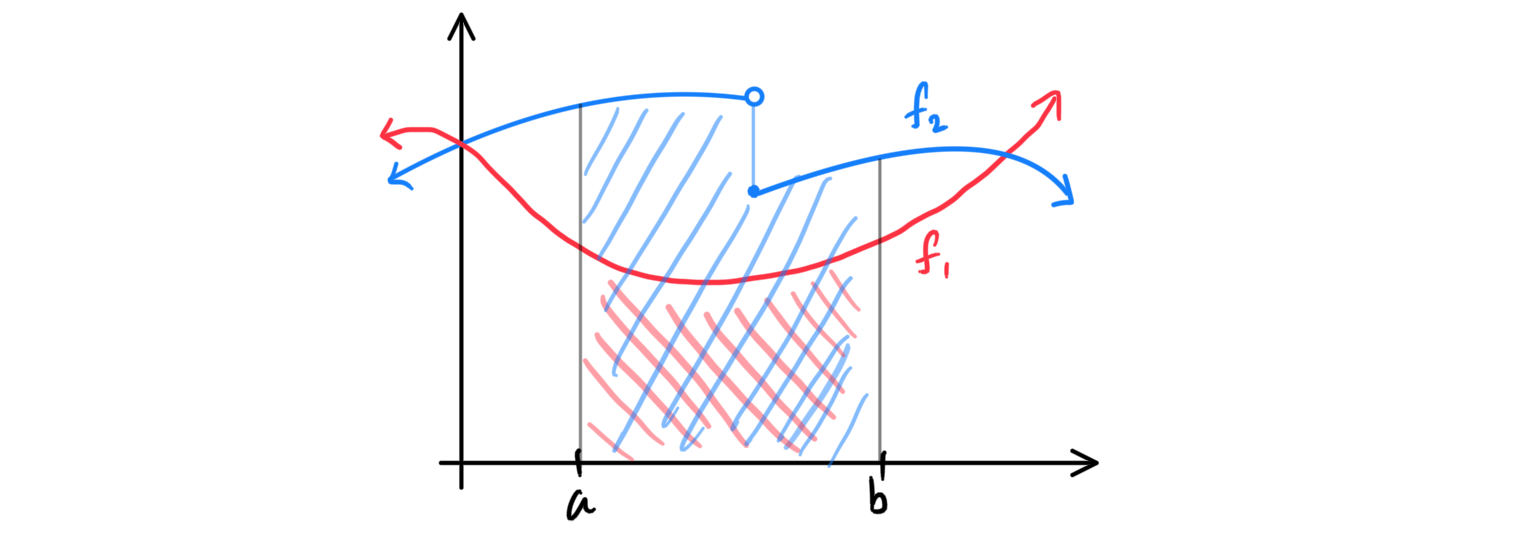
\includegraphics[scale=0.27]{img/Monotonicity_of_Integral.PNG}
      \end{center}
      This immediately implies that given constants $m, M$ such that $m \leq f(x) \leq M$ at each $x \in [a, b]$, we have
      \[m \cdot (b - a) \leq \int_a^b f(x)\,dx \leq M \cdot (b-a)\]
      This is very easily visualized below. 
      \begin{center}
          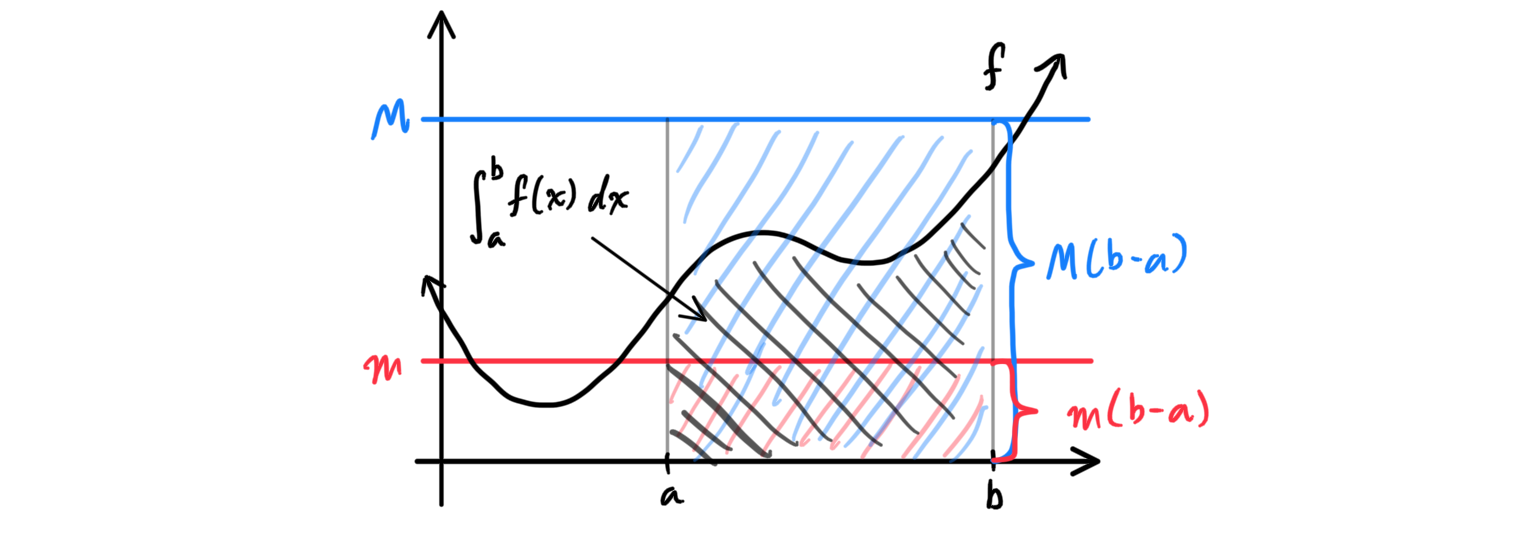
\includegraphics[scale=0.27]{img/Monotonicity_of_Intergral_2.PNG}
      \end{center}
      In particular, if $0 \leq f(x)$ on $[a, b]$, then
      \[0 \leq \int_a^b f(x)\,dx\]
    \end{lemma}

    \begin{theorem}[Mean Value Theorem of the Integral]
    Given $f \in \mathcal{R}[a, b]$, with 
    \[m = \inf_{x \in [a, b]} f(x) \text{ and } M = \sup_{x \in [a, b]} f(x)\]
    then there exists a number $\mu \in [m, M]$ such that
    \[\int_a^b f(x)\,dx = \mu \cdot (b - a)\]
    Furthermore, if $f \in C[a, b]$ (that is, continuous on $[a, b]$), it immediately follows by the intermediate value theorem that there exists a point $\xi \in [a, b]$ such that
    \[\int_a^b f(x)\,dx = f(\xi) (b - a)\]
    \begin{center}
        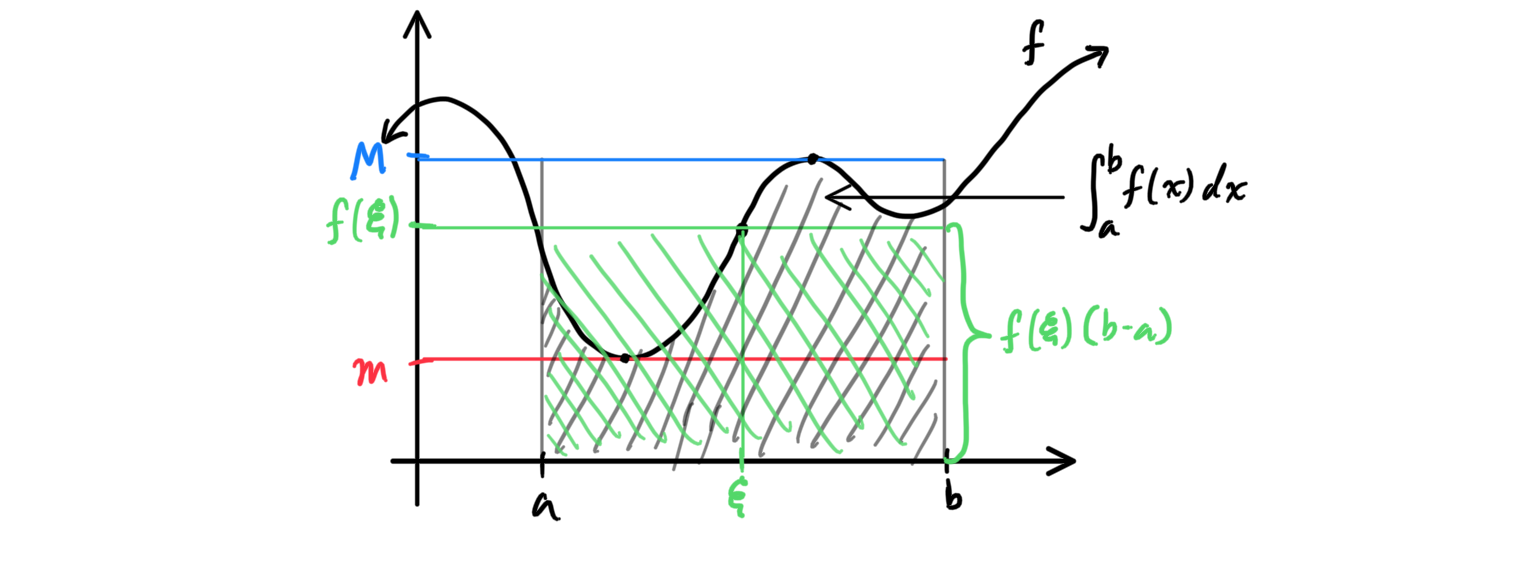
\includegraphics[scale=0.27]{img/Mean_Plus_Intermediate_Value_Theorem_Integral.PNG}
    \end{center}
    \end{theorem}

    Due to the length of the proof, we ask the reader to take it for granted the following theorem. 

    \begin{theorem}[Bonnet's Formula]
    If $f, g \in \mathcal{R}[a, b]$ and $g$ is a monotonic function on $[a, b]$, then there exists a point $\xi \in [a, b]$ such that
    \[\int_a^b (f \cdot g) (x)\,dx = g(a) \int_a^\xi f(x)\,dx + g(b) \int_\xi^b f(x)\,dx\]
    \end{theorem}

  \subsection{Connections between Integrals, Primitives, Derivatives}

    \begin{definition}[Integral with Variable Upper Limit]
      Let $f \in \mathcal{R}[a, b]$, and let us choose an $x \in [a, b]$ in order to construct the function
      \[F(x) \equiv \int_a^x f(t)\,dt\]
      which is called an \textbf{integral with variable upper limit}. Note that since $[a, x] \subset [a, b]$, it follows that $f \big|_{[a,x]} \in \mathcal{R}[a, x]$ and therefore the function $x \mapsto F(x)$ is unambiguously defined for $x \in [a, b]$. 
      \begin{center}
          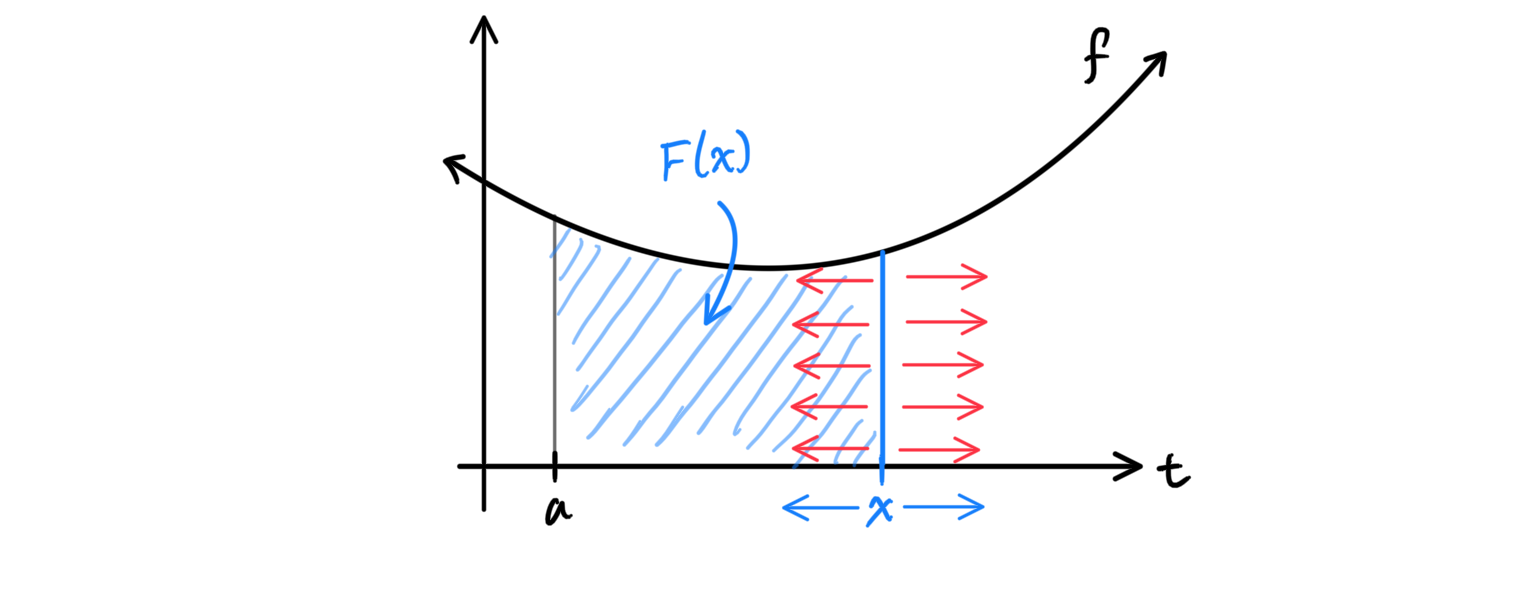
\includegraphics[scale=0.27]{img/Integral_with_Variable_Upper_Limit.PNG}
      \end{center}
      Furthermore, $F(x)$ is continuous on $[a, b]$. Since $f$ is integrable on $[a, b]$, it is bounded by a constant $C$ such that
      \[|f(t)| \leq C \text{ on } [a, b]\]
      It follows from the additive properties of the integral and boundedness theorem that 
      \[|F(x + h) - F(x)| \leq C|h|\]
      if $x, x + h \in [a, b]$, as visualized. This means that for any $\delta$-neighborhood of $F(x)$, we can find an arbitrary small $h$ such that the $C|h|$-neighborhood of $F(x)$ is completely contained in the $\delta$-neighborhood. But by the inequality above, this means that there exists an $\epsilon = h$-neighborhood of $x$ such that its entire image is contained within the $C|h|$-neighborhood, which itself is contained within the $\delta$-neighborhood. This shows that $F$ is continuous. 
    \end{definition}

    \begin{theorem}[First Fundamental Theorem of Calculus]
    Let $f \in \mathcal{R}[a, b]$ be continuous at point $x \in [a, b]$ (resp. continuous on closed interval $[a, b]$). Let $F$ be the function, defined for all $x \in [a, b]$ by 
    \[F(x) \equiv \int_a^x f(t)\,dt\]
    Then, $f$ is continuous and differentiable at $x$ (resp. uniformly continuous on $[a, b]$ and differentiable on $(a, b)$), 
    \[F^\prime (x) = f(x)\]
    at $x$ (resp. for all $x \in [a, b]$). This is an amazing fact, because visually, it tells us that the rate at which the integral $F$ is increasing at $x$ (represented by the increasing area under the curve of $f$) is equal to the value of $f$ at the point $x$ itself! 
    \begin{center}
        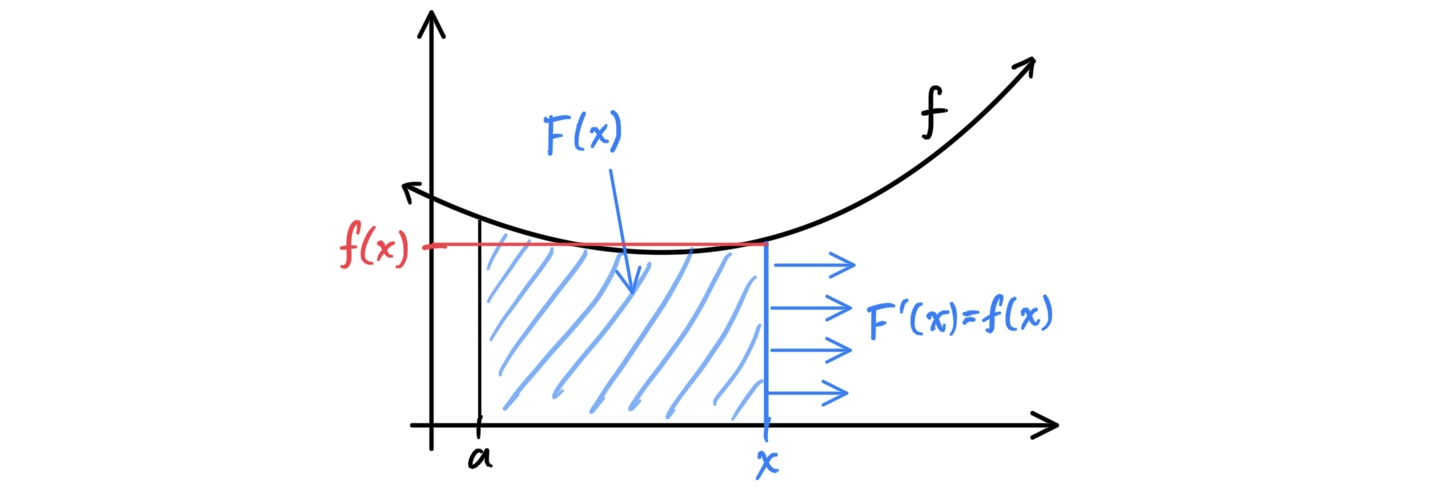
\includegraphics[scale=0.25]{img/First_Fundamental_Theorem_Analysis.jpg}
    \end{center}
    \end{theorem}
    \begin{proof}
    Let $x, x + h \in [a, b]$, and let us estimate the difference $F(x+h) - F(x)$. It follows from the continuity of $f$ at $x$ that $f(t) = f(x) + \Delta(t)$, where $\Delta(t) \rightarrow 0$ as $t \rightarrow x$. If point $x$ is held fixed, the function 
    \[\Delta(t) = f(t) - f(x)\]
    is integrable on $[a, b]$, being the difference of the integrable function $t \mapsto f(t)$ and the constant $f(x)$. Let us denote
    \[M(h) \equiv \sup_{t \in [x, x+h]} |\Delta(t)|\]
    which means that $M(h)$ is the largest difference between $f(x)$ and $f(t)$ in the interval $[x, x+h]$. 
    \begin{center}
        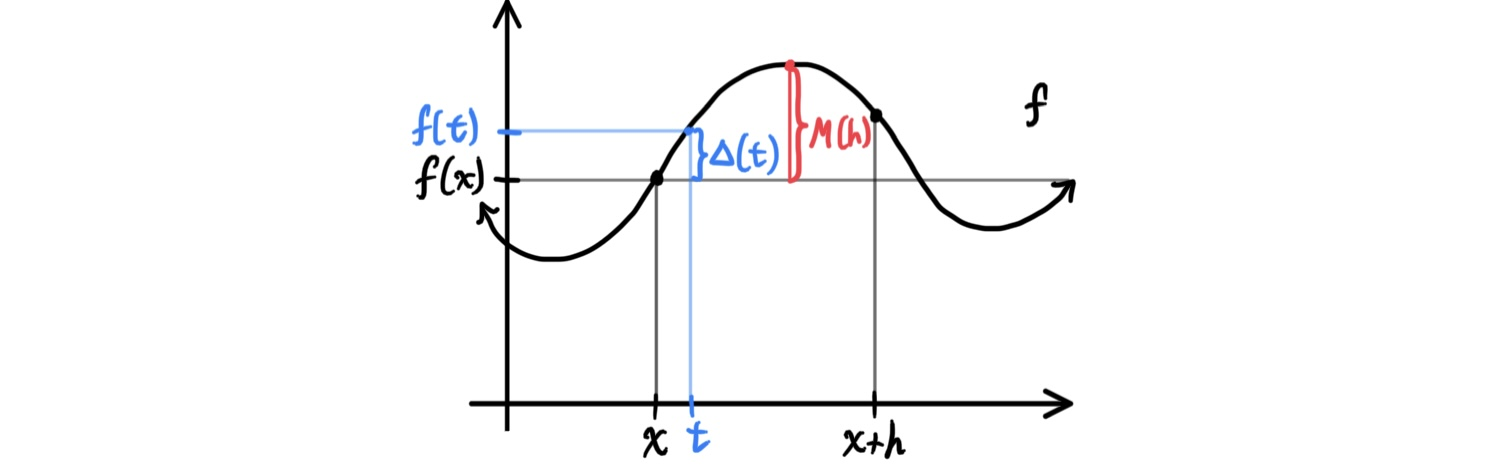
\includegraphics[scale=0.25]{img/Proof_First_Fundamental_Theorem_Analysis.jpg}
    \end{center}
    Clearly $M(h) \rightarrow 0$ as $h \rightarrow 0$. We can now find
    \begin{align*}
        F(x + h) - F(x) & = \int_a^{x+h} f(t)\,dt - \int_a^x f(t)\,dt \\
        & = \int_x^{x+h} f(t)\,dt \\
        & = \int_x^{x+h} \big( f(x) + \Delta(t)\big)\,dt \\
        & = \int_x^{x+h} f(x)\,dt + \int_x^{x+h} \Delta(t)\,dt \\
        & = f(x) h + \alpha(h) h
    \end{align*}
    where we have set 
    \[\int_x^{x+h} \Delta(t)\,dt = \alpha(h) h\]
    where $\alpha$ is infinitesimal as $h \rightarrow 0$, since 
    \[\Bigg| \int_x^{x+h} \Delta(t)\,dt \Bigg| \leq \Bigg| \int_x^{x+h} |\Delta(t)|\,dt \Bigg| \leq \Bigg| \int_x^{x+h} M(h)\,dt \Bigg| = M(h) |h| = \alpha(h)|h|\]
    Therefore, we have shown that if the function $f$ is continuous at a point $x \in [a, b]$, then for displacements $h$ from $x$ such that $x +h \in [a, b]$, the following equality holds.
    \[F(x + h) - F(x) = f(x) h + \alpha(h) h\]
    where $\alpha(h) \rightarrow 0$ as $h \rightarrow 0$, and by definition, this means that $F(x)$ is differentaible on $[a, b]$ at the point $x \in [a, b]$ and that $F^\prime(x) = f(x)$. 
    \end{proof}

    \begin{corollary}
    Every bounded function $f: [a, b] \longrightarrow \mathbb{R}$ on the closed interval $[a, b]$ and has only a finite number of points of discontinuity has a primitive, and every primitive of $f$ on $[a, b]$ has the form 
    \[\mathcal{F}(x) \equiv \int_a^x f(t)\,dt + c\]
    where $c$ is a constant. 
    \end{corollary}

    \begin{theorem}[Second Fundamental Theorem of Calculus]
    Let $f$ be a real-valued function on a closed interval $[a, b]$ with $\mathcal{F}$ any primitive of $f$ on $[a, b]$. If $f$ is Riemann-integrable (i.e. $f$ bounded with finite points of Lebesgue measure zero) on $[a, b]$, then 
    \[\int_a^b f(x)\,dx  = \mathcal{F} \big|_a^b \equiv \mathcal{F}(b) - \mathcal{F}(a)\]
    \begin{center}
        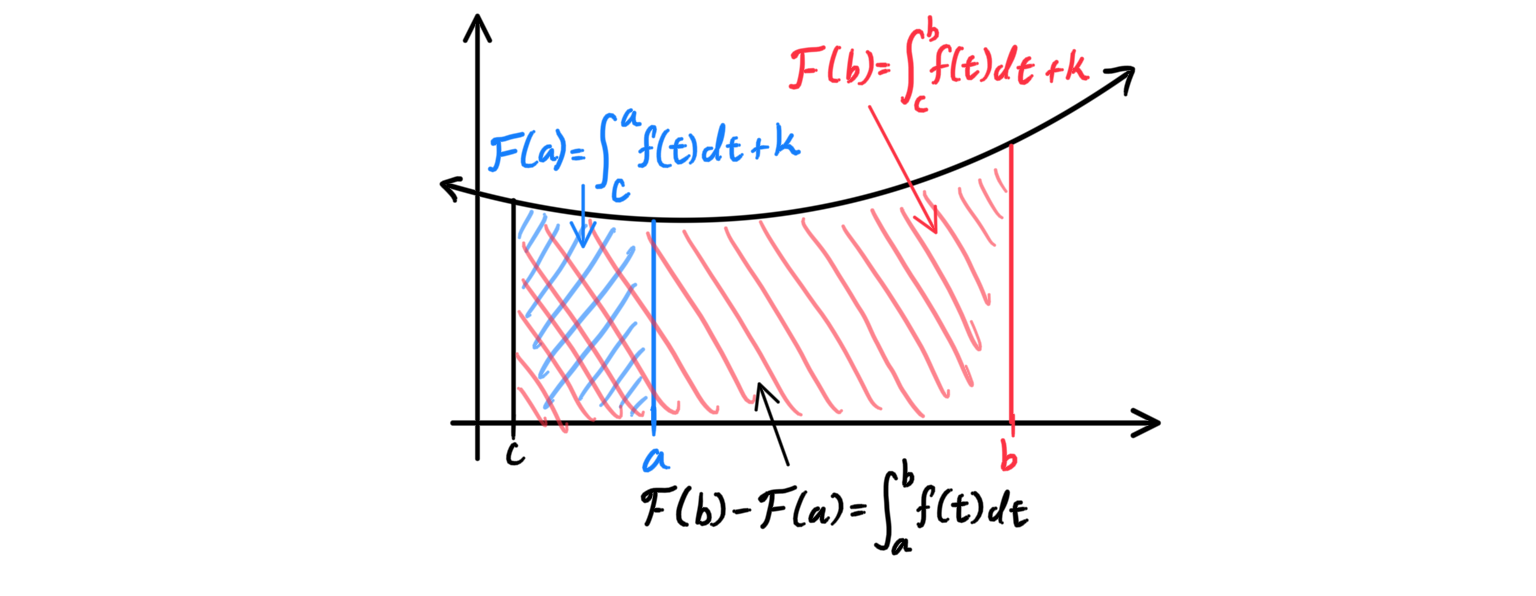
\includegraphics[scale=0.25]{img/Second_Fundamental_Theorem_Analysis.PNG}
    \end{center}
    \end{theorem}
    \begin{proof}
    We already know that a bounded function on a closed interval having a finite number of discontinuities is integrable, and by the corollary, we are guaranteed an existence of a primitive $\mathcal{F}(x)$ of the function $f$ on $[a, b]$ with the form 
    \[\mathcal{F} (x) \equiv \int_a^x f(t)\,dt + c\]
    Setting $x = a$, we find that $c = \mathcal{F}(a)$, and so 
    \[\mathcal{F}(x) \equiv \int_a^x f(t)\,dt + \mathcal{F}(a)\]
    Evaluating $\mathcal{F}$ at $x = b$ gives
    \[\int_a^b f(t)\,dt = \mathcal{F}(b) - \mathcal{F}(a)\]
    \end{proof}

    \subsubsection{Integration by Parts and Taylor's Formula}
    \begin{theorem}[Definite Integration by Parts]
    If the functions $u(x)$ and $v(x)$ are continuously differentiable on a closed interval with endpoints $a$ and $b$, then
    \[\int_a^b (u \cdot v^\prime)(x)\,dx = (u \cdot v)\big|^b_a - \int_a^b (v \cdot u^\prime)(x)\,dx\]
    which is customarily written in the form as
    \[\int_a^b u\,dv = u \cdot v \big|_a^b - \int_a^b v\,du\]
    \end{theorem}
    \begin{proof}
    By the product rule of differentiation, we have
    \[(u \cdot v)^\prime (x) = (u^\prime \cdot v)(x) + (u \cdot v^\prime) (x)\]
    where by hypothesis, $u^\prime \cdot v, u \cdot v^\prime$ are continuous and hence integrable on $[a, b]$. Using the linearity of the integral and the 2nd fundamental theorem of calculus, we get
    \[(u \cdot v) (x) \big|^b_a = \int_a^b (u^\prime \cdot v)(x)\,dx + \int_a^b (u \cdot v^\prime) (x)\,dx\]
    \end{proof}

    \begin{theorem}[Integral Form of the Remainder]
    If $f: E \longrightarrow \mathbb{R}$ has continuous derivatives up to order $n$ on the closed interval $[a, x]$, then Taylor's formula holds
    \[f(x) = f(a) + \frac{f^\prime (a)}{1!} (x - a) + \ldots + \frac{f^{(n-1)}(a)}{(n-1)!} (x - a)^{n-1} + r_{n-1}(a; x)\]
    where 
    \[r_{n-1} (a;x) = \frac{1}{(n-1)!} \int_a^x f^{(n)} (t) (x - t)^{n-1} \,dt\]
    This form is called \textbf{Taylor's formula with the integral form of the remainder}. 
    \end{theorem}
    \begin{proof}
    Using the 2nd fundamental theorem and the definite integration by parts formula, we can carry out the following chain of transformations, assuming continuity and differentiability when needed. 
    \begin{align*}
        f(x) - f(a) & = \int_a^x f^\prime (t) \,dt \\
        & = - \int_a^x f^\prime(t) (x - t)^\prime \,dt \\
        & = -f^\prime (t) (x - t)\big|_a^x + \int_a^x f^{\prime\prime} (t) (x - t) \,dt \\
        & = f^\prime (a) (x - a) - \frac{1}{2} \int_a^x f^{\prime\prime} (t) \big( (x - t)^2\big)^\prime \,dt \\
        & = f^\prime (x - a) - \frac{1}{2} f^{\prime\prime} (t) (x - t)^2 \big|_a^x + \frac{1}{2} \int_a^x f^{\prime\prime\prime} (t) (x - t)^2\,dt \\
        & = f^\prime(a) (x - a) + \frac{1}{2} f^{\prime\prime} (a) (x - a)^2 - \frac{1}{2 \cdot 3} \int_a^x f^{\prime\prime\prime} (t) \big((x - t)^3\big)^\prime\,dt \\
        & = \ldots \\
        & = f^\prime (a) (x - a) + \ldots + \frac{1}{(n-1)!} f^{(n-1)} (a)(x - a)^{n-1} + r_{n-1}(a;x)
    \end{align*}
    where $r_{n-1}(a;x)$ is given by the integral formula mentioned. 
    \end{proof}

    \subsubsection{Change of Variables in Integration}
    We now show and prove the method what we call "u-substitution" for definite integration. 

    \begin{theorem}[Change of Variable]
    If $\varphi: [\alpha, \beta] \longrightarrow [a, b]$ is a continuously differentiable mapping such that $\varphi(\alpha) = a$ and $\varphi(\beta) = b$, then for any continuous function $f(x)$ on $[a, b]$ the function $f\big(\varphi(t)\big) \varphi^\prime (t)$ is continuous on the closed interval $[\alpha, \beta]$ and 
    \[\int_a^b f(x)\,dx = \int_\alpha^\beta f\big(\varphi(t)\big) \varphi^\prime(t)\,dt\]
    \begin{center}
        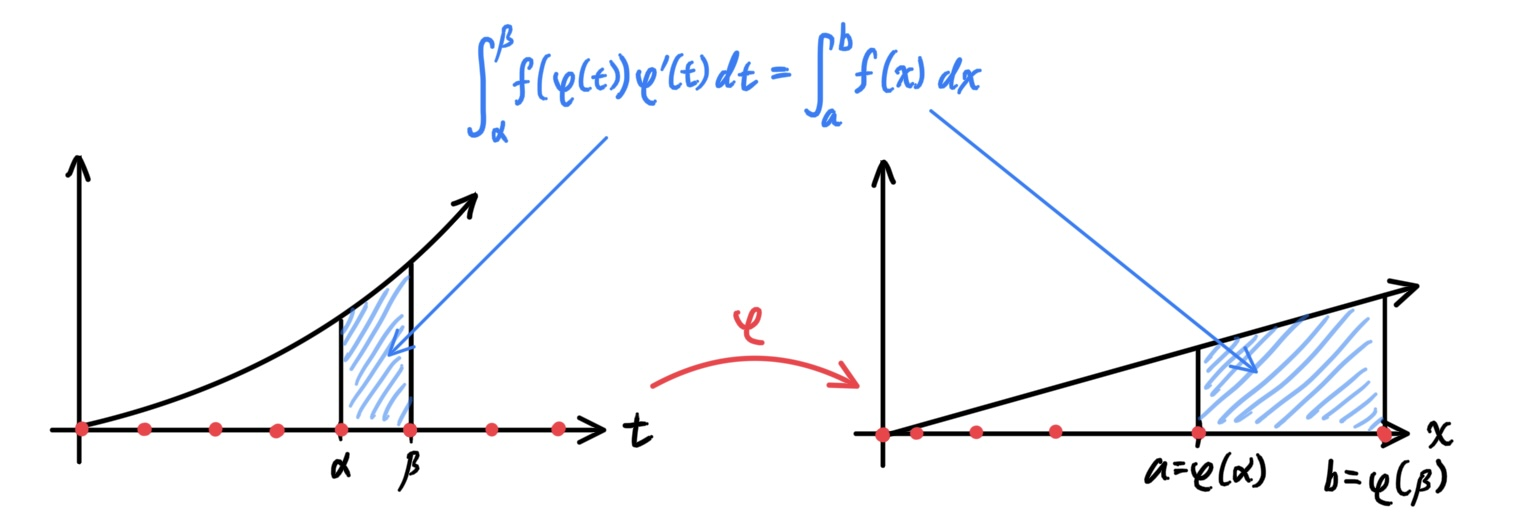
\includegraphics[scale=0.25]{img/Change_of_Variable_Analysis_Integral.jpg}
    \end{center}
    \end{theorem}
    \begin{proof}
    We prove a slightly weaker form of the theorem with the additional hypothesis that $\varphi$ is strictly monotonic. 
    \end{proof}

    \subsubsection{Additive Interval Functions and the Integral}
    In this section we take a step back and construct the integral in a more abstract sense, using the concepts of an additive interval function. 

    \begin{definition}[Additive Interval Function]
      An \textbf{additive (oriented) interval function} is a function 
      \[(\alpha, \beta) \mapsto I(\alpha, \beta) \in \mathbb{R}\]
      that assigns a number $I(\alpha, \beta)$ to each ordered pair of points $(\alpha, \beta)$ of a fixed closed interval $[a, b]$ in such a way that the following equality holds for any triple of points $\alpha, \beta, \gamma \in [a, b]$. 
      \[I(\alpha, \gamma) = I(\alpha, \beta) + I(\beta, \gamma)\]
      Notice that the integral holds this property, shown in the theorem on the symmetric property of the integral. It follows that all additive interval functions are anticommutative: 
      \[I(\alpha, \beta) + I(\beta, \alpha) = 0\]
      which immediately results in
      \[I(\alpha, \alpha) = 0\]
    \end{definition}

    \begin{lemma}[Generating Functions of Additive Interval Functions]
      For any function $x \mapsto \mathcal{F}(x)$ that maps points on the interval $[a, b]$ to $\mathbb{R}$, we set
      \[\mathcal{F}(x) \equiv I(a, x)\]
      and by additivity we have
      \[I(\alpha, \beta) = I(\alpha, \beta) - I(a, \alpha) = \mathcal{F}(\beta) - \mathcal{F}(\alpha)\]
      and thus, every additive oriented interval function has the form 
      \[I(\alpha, \beta) = \mathcal{F}(\beta) - \mathcal{F}(\alpha)\]
      By constructing $I$ in this manner, we say that \textbf{the function $\mathcal{F}$ generates the additive function $I$}. 
    \end{lemma}

    \begin{example}
    If $f \in \mathcal{R}[a, b]$, the function $\mathcal{F} = \int_a^x f(t)\,dt$ generates the additive function
    \[I(\alpha, \beta) = \mathcal{F}(\beta) - \mathcal{F}(\alpha) = \int_a^\beta f(t)\,dt - \int_a^\alpha f(t)\,dt = \int_\alpha^\beta f(t)\,dt\]
    \end{example}

    We conclude by stating a sufficient condition for an additive interval function to be generated by an integral. 
    \begin{theorem}
    Suppose the additive function $I(\alpha, \beta)$ defined for points $\alpha, \beta \in [a, b]$ has the property that, for some known function $f \in \mathcal{R}[a, b]$, 
    \[\inf_{x \in [\alpha, \beta]} f(x) (\beta - \alpha) \leq I(\alpha, \beta) \leq \sup_{x \in [\alpha, \beta]} f(x) (\beta - \alpha)\]
    holds for any closed interval $[\alpha, \beta] \subset [a, b]$ ($\alpha \leq \beta$). Then, the additive function $I$ must be the definite integral
    \[I(a, b) = \int_a^b f(x)\,dx\]
    \end{theorem}

    This theorem is extremely useful. It says that if we have any abstract additive interval function $I(\alpha, \beta)$ that satisfies the properties above, then it \textbf{must} be generated by an integral with variable upper limit, meaning that (by the previous example) $I$ itself must be a definite integral! 

    \subsubsection{Arc Length}
    When modeling systems in physics, one of the most fundamental tools we use are path functions that models the movement of a particle in $\mathbb{R}^3$. 

    \begin{definition}[Path]
      A \textbf{path} in $\mathbb{R}^3$ is a continuous mapping $r: [a, b] \subset \mathbb{R} \longrightarrow \mathbb{R}^3$ defined
      \[t \mapsto \big(x(t), y(t), z(t)\big)\]
      of an interval of the real line into $\mathbb{R}^3$ defined by the (continuous) scalar functions $x, y, z$. The endpoints 
      \[A = \big(x(a), y(a), z(a)\big) \text{ and } B = \big(x(b), y(b), z(b)\big)\]
      in $\mathbb{R}^3$ are called the \textbf{initial point} and \textbf{terminal point} of the path. Furthermore, a path is \textbf{closed} if its initial and terminal points coincide. 
    \end{definition}

    \begin{definition}[Support]
      If $\Gamma: I \longrightarrow \mathbb{R}^3$ is a path, the image $\Gamma(I) \subset \mathbb{R}^3$ is called the \textbf{support} of the path. 
    \end{definition}

    \begin{definition}[Simple Paths]
      A path $\Gamma: I \longrightarrow \mathbb{R}^3$ that is injective is called a \textbf{simple path}, or a \textbf{paramaterized curve}, and its support is called a \textbf{curve} in $\mathbb{R}^3$. 

      A closed path $\Gamma: [a, b] \longrightarrow \mathbb{R}^3$ is called a \textbf{simple closed path/curve} if the path $\Gamma: [a, b) \longrightarrow \mathbb{R}^3$ is simple. 
    \end{definition}

    \begin{definition}[Smooth Paths]
      A path $\Gamma: [a, b] \longrightarrow \mathbb{R}^3$ is $C^k$ smooth if the functions $x(t), y(t), z(t)$ are $C^k$ smooth. $\Gamma$ is \textbf{piecewise smooth} if the closed interval $[a, b]$ can be partitioned into a finite number of closed intervals on each of which the corresponding restriction of $\Gamma$ is smooth. 
    \end{definition}

    Now, we are ready to construct the length of a smooth path $\Gamma: [a, b] \longrightarrow \mathbb{R}^3$. Our initial ideas about the length $l[a, b]$ of the path traversed during the time interval $\alpha \leq t \leq \beta$ are as follows: 
    \begin{enumerate}
      \item If $\alpha < \beta < \gamma$, then $l$ is an additive interval function.
      \[l[\alpha, \gamma] = l[\alpha, \beta] + l[\beta, \gamma]\]
      \item If $v(t) = \big( x^\prime (t), y^\prime (t), z^\prime (t)\big)$ is the velocity of the point at time $t$, then 
      \[\int_{x \in [\alpha, \beta]} |v(t)| (\beta - \alpha) \leq l[\alpha, \beta] \leq \sup_{x \in [\alpha, \beta]} |v(t)| (\beta - \alpha)\]
    \end{enumerate}
    Thus, if the functions $x, y, z$ are continuously differentiable on $[a, b]$, this is sufficient condition (by the theorem in the previous subsection) that the additive function $l$ is an integral.

    \begin{definition}[Arc Length Integral]
      The length of a smooth path $\Gamma: [a, b] \longrightarrow \mathbb{R}^3$ is defined by 
      \[l[a, b] \equiv \int_a^b |\Gamma^\prime (t)|\,dt \equiv \int_a^b \sqrt{x^{\prime 2} (t) + y^{\prime 2} (t) + z^{\prime 2} (t)}\, dt\]
      We can visualize this by partitioning the interval $[a, b]$ into the intervals $\Delta_i$, each with point $\xi_i \in \Delta_i$. This would partition the path to $\Gamma(\Delta_i)$, each with points $\Gamma(\xi_i)$, and at each point $\Gamma(\xi_i)$, we can imagine the velocity vector of the curve. By taking the magnitude of this vector $\Gamma^\prime (\xi_i)$, we multiply it by the length of the interval $\Delta x_i$ to get one rectangle, creating an approximation for one partition of the path. 
      \begin{center}
          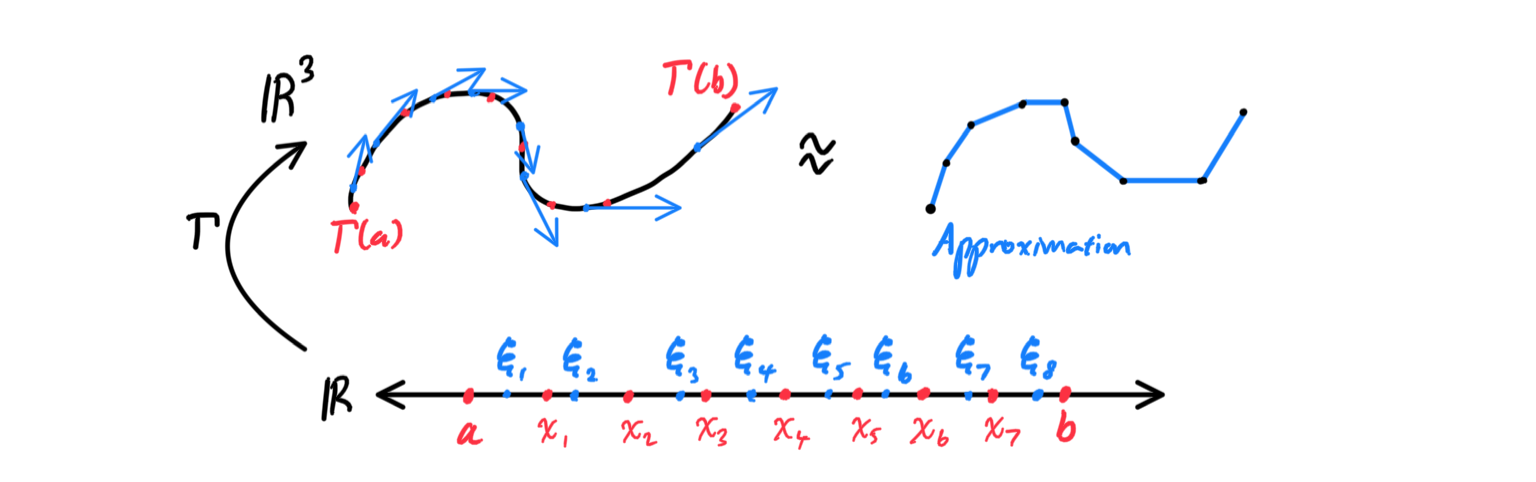
\includegraphics[scale=0.25]{img/Arc_Length_Integral.PNG}
      \end{center}
      An immediate result of this formula is the formula for the length of a graph of a function $f: [a, b] \longrightarrow \mathbb{R}$ in $\mathbb{R}^2$, by looking at the paramaterization $t \mapsto \Gamma(t) = \big(t, f(t)\big)$. 
      \[l[a,b] \equiv \int_a^b \sqrt{1 + (f^\prime (t))^2}\,dt\]
    \end{definition}

    The question on the effect of paramaterization on the integral now arises. 

    \begin{definition}[Admissible Change of Parameter]
      The path $\Tilde{\Gamma}: [\alpha, \beta] \longrightarrow \mathbb{R}^3$ is obtained from $\Gamma: [a, b] \longrightarrow \mathbb{R}^3$ by an \textbf{admissible change of parameter} if there exists a smooth mapping 
      \[T: [\alpha, \beta] \longrightarrow [a, b]\]
      such that $T(\alpha) = a, T(\beta) = b$, $T^\prime (\tau) > 0$ (that is, the reparamaterization $T$ is monotonic) on $[\alpha, \beta]$, and 
      \[\Tilde{\Gamma} = \Gamma \circ T\]
      The series of mappings can be represented with the following commutative diagram, where $I_{\alpha, \beta} = [\alpha, \beta] \subset \mathbb{R}$ and $I_{a, b} = [a, b] \subset \mathbb{R}$. 
      \[
        \begin{tikzcd}
          I_{\alpha, \beta} \arrow{r}{T} \arrow{rd}{\Tilde{\Gamma}}& I_{a, b} \arrow{d}{\Gamma}\\
           & \mathbb{R}^3
        \end{tikzcd}
      \]
      or with the more detailed visual below (Note that the points are labeled $0, 1, 2, 3, 4, 5$ do not represent numerical values, but rather the order in which the points are paramaterized. We can see from this ordering that $T$ is monotonic.)
      \begin{center}
          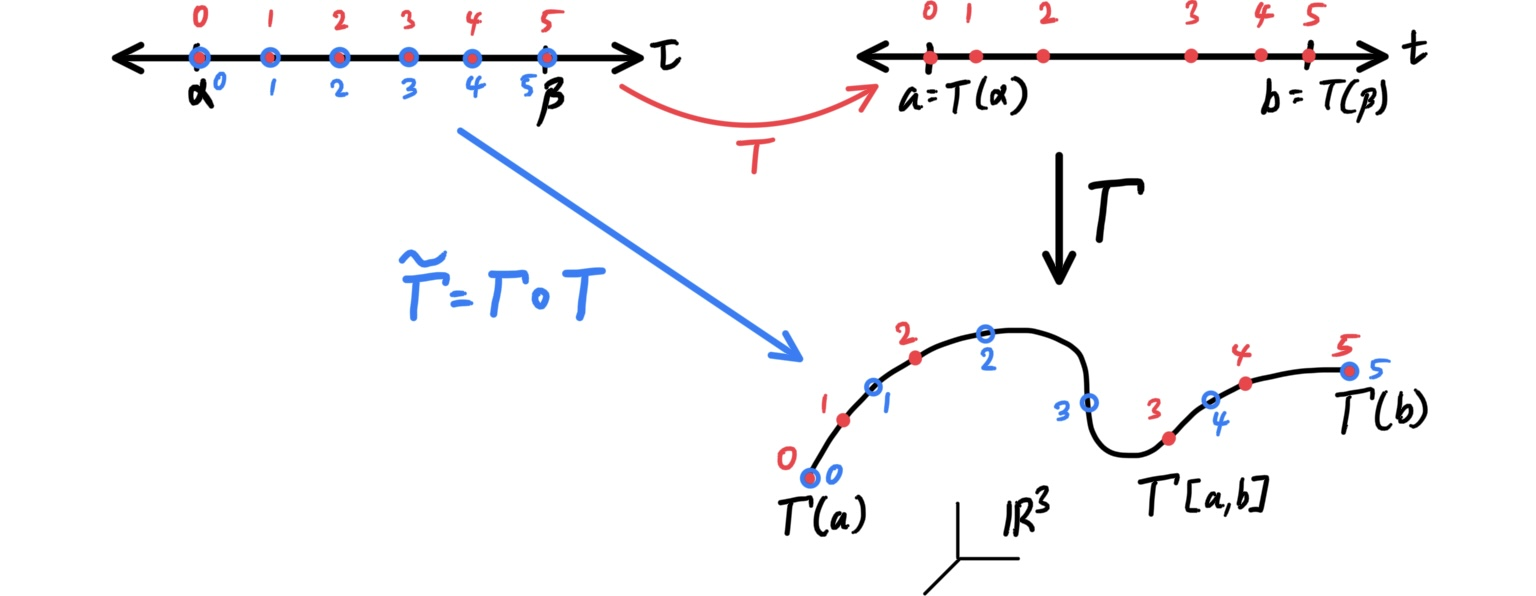
\includegraphics[scale=0.25]{img/Admissible_Change_of_Parameter.jpg}
      \end{center}
    \end{definition}

    \begin{theorem}[Invariance of Arclength Integral under Admissible Change of Parameters]
    If a smooth path $\Tilde{\Gamma}: [\alpha, \beta] \longrightarrow \mathbb{R}^3$ is obtained from a smooth path $\Gamma: [a, b] \longrightarrow \mathbb{R}^3$ by an admissible change of parameter, then the lengths of the two paths are equal. That is, a
    \[\int_a^b |\Gamma^\prime (t) |\,dt = \int_\alpha^\beta |\Tilde{\Gamma}^\prime (t)|\,dt \equiv \int_\alpha^\beta |(\Gamma \circ T)^\prime (t)|\,dt\]
    \end{theorem}

  \subsection{Improper Integrals}

    Due to some limitations of the Riemann integral, we cannot integrate over "singularities" where either the interval or the function is unbounded. We develop the tools of improper integration to deal with this problem; there are two types of improper integrals. 

    \begin{definition}[Improper Integral of Unbounded Interval]
      Suppose the function $x \mapsto f(x)$ is defined on the interval $[a, +\infty)$ and is integrable on every closed interval $[a, b]$ contained in that interval. Then, we call the following term
      \[\int_a^{+\infty} f(x)\,dx \equiv \lim_{b \rightarrow + \infty} \int_a^b f(x)\,dx\]
      the \textbf{improper Riemann integral of $f$ over the interval $[a, +\infty)$} and 
      \[\int_{-\infty}^b f(x)\,dx \equiv \lim_{a \rightarrow -\infty} \int_a^b f(x)\,dx \]
      the \textbf{improper Riemann integral of $f$ over the interval $(-\infty, b]$}.If the limit exists, then we say that the integral \textbf{converges} and \textbf{diverges} otherwise. 
    \end{definition}

    \begin{definition}[Improper Integral of Unbounded Function]
      Suppose the function $x \mapsto f(x)$ is defined on the interval $[a, B)$ and integrable on any closed interval $[a, b] \subset [a, B)$. Then, we call the following term
      \[\int_a^B f(x)\,dx \equiv \lim_{b \rightarrow B^-} \int_a^b f(x)\,dx\]
      the \textbf{improper Riemann integral of $f$ over interval $[a, B)$} and
      \[\int_A^b f(x)\,dx \equiv \lim_{a \rightarrow A^+} \int_a^b f(x)\,dx\]
      the \textbf{improper Riemann integral of $f$ over interval $(A,b]$}.
    \end{definition}

    For cohesiveness, we can combine these two definitions of improper integrals into the following one. 

    \begin{definition}[Improper Integrals]
      Let $[a, \omega)$ be a finite or infinite interval and $x \mapsto f(x)$ a function defined on that interval and integrable over every closed interval $[a, b] \subset [a, \omega)$. Then, by definition
      \[\int_a^\omega f(x)\,dx \equiv \lim_{b \rightarrow \omega} \int_a^b f(x)\,dx\]
      if this limit exists as $b \rightarrow \omega, b \in [a, \omega)$. Similarly, given the finite or infinite interval $(\omega, b]$ with $f$ integrable over every closed interval $[a, b] \subset (\omega, b]$, we have
      \[\int_\omega^b f(x)\,dx \equiv \lim_{a \rightarrow \omega} \int_a^b f(x)\,dx\]
      Note that if $\omega \in \mathbb{R}$ and $f \in \mathcal{R}[a, \omega]$, the improper integral is equivalent to the regular Riemann integral. 
      \[\int_a^\omega f(x) = \lim_{b\rightarrow \omega} \int_a^b f(x)\,dx\]
    \end{definition}

    \begin{lemma}[Properties of the Improper Integral]
      Suppose $f, g$ are functions defined on interval $[a, \omega)$ (without loss of generality, we let $\omega$ be the upper limit of integration) and integrable on every closed interval $[a, b] \subset [a, \omega)$. Suppose the improper integrals 
      \[\int_a^\omega f(x)\,dx \text{ and } \int_a^\omega g(x)\,dx\]
      are well-defined. 
      \begin{enumerate}
        \item For any $\lambda_1, \lambda_2 \in \mathbb{R}$ the function $(\lambda_1 f + \lambda_2 g)(x)$ is integrable in the improper sense on $[a, \omega)$ and
        \[\int_a^\omega (\lambda_1 f + \lambda_2 g)(x)\,dx = \lambda_1 \int_a^\omega f(x)\,dx + \lambda_2 \int_a^\omega g(x)\,dx\]
        \item For any $c \in [a, \omega)$, 
        \[\int_a^\omega f(x)\,dx = \int_a^c f(x)\,dx + \int_c^\omega f(x)\,dx\]
        \item If $\varphi: [\alpha, \gamma) \longrightarrow [a, \omega)$ is a smooth strictly monotonic mapping with $\varphi(\alpha) = a$ and $\varphi(\beta) \rightarrow \omega$ as $\beta \rightarrow \gamma^-$, then the improper integral of the function $t \mapsto (f \circ \varphi)(t) \varphi^\prime (t)$ over $[\alpha, \gamma)$ exists and 
        \[\int_a^\omega f(x)\,dx = \int_\alpha^\gamma (f \circ \varphi)(t) \varphi^\prime (t)\,dt\]
      \end{enumerate}
    \end{lemma}

    \subsubsection{Convergence of an Improper Integral}

      Note that by definition, an improper integral 
      \[\int_a^\omega f(x)\,dx \equiv \lim_{b \rightarrow \omega} \int_a^b f(x) \,dx\]
      is a limit of the function 
      \[\mathcal{F}(b) \equiv \int_a^b f(x)\,dx\]
      as $b \rightarrow \omega$. This means that we can use the Cauchy criterion to determine the convergence of this limit, and hence, existence of this improper integral. 

      \begin{theorem}[Cauchy Criterion for Convergence of an Improper Integral]
      If the function $x \mapsto f(x)$ is defined on the interval $[a, \omega)$ and integrable on every closed interval $[a, b] \subset [a, \omega)$, then the integral 
      \[\int_a^\omega f(x)\,dx\]
      converges if and only if for every $\epsilon > 0$ there exists $B \in [a, \omega)$ such that the relation
      \[\Bigg| \int_{b_1}^{b_2} f(x)\,dx \bigg| < \epsilon\]
      holds for any $b_1, b_2 \in [a, \omega)$ satisfying $B < b_1$ and $B < b_2$. 
      \end{theorem}
      \begin{proof}
      We have
      \[\int_{b_1}^{b_2} f(x)\,dx = \int_a^{b_2} f(x)\,dx - \int_a^{b_1} f(x)\,dx = \mathcal{F}(b_2) - \mathcal{F}(b_1)\]
      and therefore the condition is simply the Cauchy criterion for the existence of a limit for the function $\mathcal{F}(b)$ as $b \rightarrow \omega$. 
      \end{proof}

      \begin{definition}[Absolute Convergence of an Improper Integral]
        The improper integral 
        \[\int_a^\omega f(x)\,dx\]
        \textbf{converges absolutely} if the integral
        \[\int_a^\omega |f|(x)\,dx\]
        converges. Clearly, the inequality
        \[\Bigg| \int_{b_1}^{b_2} f(x)\,dx \Bigg| \leq \Bigg| \int_{b_1}^{b_2} |f|(x)\,dx \Bigg|\]
        implies that if an improper integral converges absolutely, then it converges. 
      \end{definition}

      This study of absolute convergence reduces to the study of convergence of integrals of nonnegative functions. The following lemma is useful in determining convergence of such functions. 

      \begin{lemma}
        Let there be a function $f$ defined on interval $[a, \omega)$ that is also integrable over every closed interval $[a, b] \subset [a, \omega)$. If $f(x) \geq 0$ on $[a, \omega)$, then the improper integral 
        \[\int_a^\omega f(x)\,dx\]
        exists if and only if the function 
        \[\mathcal{F}(b) \equiv \int_a^b f(x)\,dx\]
        is bounded on $[a, \omega)$. 
      \end{lemma}
      \begin{proof}
      It is clear that 
      \[\int_a^\omega f(x)\,dx = \lim_{b \rightarrow \omega} \mathcal{F}(b)\]
      If $f(x)\geq 0$, then the function $\mathcal{F}(b)$ is nondecreasing on $[a, \omega)$ and therefore has a limit as $b \rightarrow \omega$ only if it is bounded (since every monotonically increasing sequence that is bounded always converges). 
      \end{proof}

      This leads to the familiar integral test for convergence of a series. 

      \begin{theorem}[Integral Test for Convergence of a Series]
      If the function $x \mapsto f(x)$ is defined on the interval $[1, +\infty)$, nonnegative, nonincreasing, and integrable on each closed interval $[1, b] \subset [1, +\infty)$, then the series 
      \[\sum_{n=1}^\infty f(n) = f(1) + f(2) + \ldots\]
      and the integral 
      \[\int_a^{+\infty} f(x)\,dx\]
      either both converge or both diverge. 
      \end{theorem}

      We can use the comparison test analogue to determine convergence of improper integrals. 

      \begin{theorem}[Comparison Test for Convergence of Improper Integrals]
      Suppose the functions $f(x), g(x)$ are defined on the interval $[a, \omega)$ and integrable on any closed interval $[a, b] \subset [a, \omega)$. If 
      \[0 \leq f(x) \leq g(x)\]
      on $[a, \omega)$, then 
      \[\int_a^\omega g(x)\,dx \text{ converges} \implies \int_a^\omega f(x)\,dx \text{ converges}\]
      and the inequality 
      \[\int_a^\omega f(x)\,dx \leq \int_a^\omega g(x)\,dx\]
      holds. Also, 
      \[\int_a^\omega f(x)\,dx \text{ diverges} \implies \int_a^\omega g(x)\,dx \text{ diverges}\]
      \end{theorem}
    
    \subsubsection{Improper Integrals with Multiple Singularities}

      \begin{definition}[Improper Integral with Both Limits as Singularities]
        Given singularities $\omega_1, \omega_2$, the improper integral is defined
        \[\int_{\omega_1}^{\omega_2} f(x)\,dx \equiv \int_{\omega_1}^c f(x)\,dx + \int_c^{\omega_2} f(x)\,dx\]
        where $c$ is an arbitrary point in $(\omega_1, \omega_2)$. 
      \end{definition}

    \begin{example}[Gaussian Integral]
    The integral 
    \[\int_{-\infty}^{+\infty} e^{-x^2}\,dx = \sqrt{\pi}\]
    \end{example}

 

\end{document}
